%%%%%%%%%%%%%%%%%%%%%%%%%%%%%%%%%%%%%
%% Master file SED-ML specification 
%%%%%%%%%%%%%%%%%%%%%%%%%%%%%%%%%%%%%
\listfiles
\documentclass[pdftex,rgb,dvipsnames,svgnames,hyperref,table]{report}
\usepackage{tocvsec2} 

% layout (initialy done for the SBGN project)
%% ----------------------------------------------------------------------------
%% Load up packages we need.
%% ----------------------------------------------------------------------------

% Warning: more \usepackage commands are used later in this file.

\usepackage[a4paper,centering,margin=1in,marginparwidth=0.75in]{geometry}
\usepackage[utf8]{inputenc} % unicode support
\usepackage{shadow}
\usepackage{supertabular}
\usepackage{multirow}
\usepackage{multicol}
\usepackage{enumitem}
\usepackage{lscape}
\usepackage{layout}
\usepackage{array}
\usepackage{fancybox}
\usepackage{xspace}
\usepackage{ifpdf}

% Hyperref, xcolor, graphicx and possibly others have a flag "pdftex"
% that needs to be used if pdflatex is being used.  The following puts
% these inside a conditional for that situation.

\ifpdf
  % Case: using pdflatex
  \usepackage[pdftex,rgb,dvipsnames,svgnames,hyperref,table]{xcolor}

\else
  % Case: not using pdflatex
  \usepackage[rgb,dvipsnames,svgnames,hyperref,table]{xcolor}

\fi


\usepackage{float}
\usepackage[american]{varioref}
\usepackage[normalem]{ulem}
\usepackage{eso-pic}                   
\usepackage{natbib}
\usepackage{listings} % enabling listings

\usepackage{url} % enabling URLs


\usepackage{pifont}% enable dingbats
\usepackage{alltt}


% package to enanble metapost for drawing the UML classes
\usepackage{emp}
% use: mpost spec.mp to create the UML diagrams

%\usepackage{enumerate}
% to change enumeration starting numbers and so on

%\usepackage{color} % enabling text colors

% using pdflatex with emp package
 \ifx\pdftexversion\undefined
 \usepackage[dvips]{graphicx}
 \else
 \usepackage[pdftex]{graphicx}
 \graphicspath{{./}{./images/}}
\DeclareGraphicsExtensions{.png}
 \DeclareGraphicsRule{*}{mps}{*}{}
 \fi

% Hyperref, xcolor, graphicx and possibly others have a flag "pdftex"
% that needs to be used if pdflatex is being used.  The following puts
% these inside a conditional for that situation.

\ifpdf
  % Case: using pdflatex

  \usepackage[pdftex]{graphicx}
  \DeclareGraphicsExtensions{.pdf,.png}

  % Options get even more complicated.  If we're producing grayscale output,
  % we don't want to bother with coloring links, but we still want to load
  % hyperref so that its macros are defined (and we don't have to redefine
  % everything that uses hyperref).  So:

  \usepackage[pdftex,breaklinks=true,colorlinks=true,plainpages=false,
  pdfpagelabels,bookmarks=true,bookmarksopen=true,bookmarksopenlevel=2,
  pdfhighlight=/O,linkcolor={RoyalBlue},citecolor={RoyalBlue},
  urlcolor={RoyalBlue}]{hyperref}

  \usepackage[pdftex,rgb,dvipsnames,svgnames,hyperref,table]{xcolor}

\else
  % Case: not using pdflatex

  \usepackage{graphicx}
  \DeclareGraphicsExtensions{.eps,.png}

  \usepackage[breaklinks,plainpages=false,pdfpagelabels]{hyperref}
  \usepackage[rgb,dvipsnames,svgnames,hyperref,table]{xcolor}

\fi

% Package 'rotating' needs to come after the others.

\usepackage{rotating}

% Booktabs for sharp-looking \toprule, \midrule, \bottomrule in tables.

\usepackage{booktabs}
\setlength{\cmidrulewidth}{0.3 pt}
\setlength{\lightrulewidth}{0.3 pt}
\setlength{\heavyrulewidth}{0.9 pt}
\setlength{\parindent}{0pt} % no indents in the whole document

%% ----------------------------------------------------------------------------
%% Special customizations
%% ----------------------------------------------------------------------------


\makeatletter

% Adjust bottom-of-page behavior and page line spacing.

\raggedbottom
\renewcommand{\baselinestretch}{0.98}

% Numbers the paragraph, but does not lists them in the ToC

\setcounter{secnumdepth}{4}
\setcounter{tocdepth}{2}

% Fix placement of figures & tables.  This keeps latex from shoving big
% floats to the end of a document when they are somewhat big, which it will
% do even if you put [htb] as the argument.

\setcounter{topnumber}{3}
\renewcommand\topfraction{1.0}
\setcounter{bottomnumber}{2}
\renewcommand\bottomfraction{1.0}
\renewcommand\textfraction{0.0}
\renewcommand\floatpagefraction{0.9}

% Adjustment to the spacing around tables and figures.

\renewcommand{\intextsep}{2em}

% This sets up Helvetica for headings.  The font scaling is
% because the default Helvetica size is too big.

\RequirePackage{helvet}
\def\Hv@scale{0.87}

% The following sets up txtt for the typewriter font.

\renewcommand{\ttdefault}{txtt}
\DeclareMathAlphabet{\mathtt}{OT1}{txtt}{m}{n}
\SetMathAlphabet{\mathtt}{bold}{OT1}{txtt}{b}{n}

% The next bit is an adaption of code from ot1phv.fd and adapted to the txtt
% fonts.  The txtt fonts are just a tad too big, so this tries to rescale
% them down a tiny bit.  This isn't completely right because I couldn't
% figure out the right syntax when the DeclareFontShape uses ssub below.
% (Notice how the ones with ssub don't have the \Txtt@@scale factor.)

\def\Txtt@scale{0.975}
\edef\Txtt@@scale{s*[\csname Txtt@scale\endcsname]}%

\DeclareFontFamily{OT1}{txtt}{\hyphenchar \font\m@ne}
\DeclareFontShape{OT1}{txtt}{m}{n}{	%rebular
     <-> \Txtt@@scale txtt%
}{}
\DeclareFontShape{OT1}{txtt}{m}{sc}{	%cap & small cap
     <-> \Txtt@@scale txttsc%
}{}
\DeclareFontShape{OT1}{txtt}{m}{sl}{	%slanted
     <-> \Txtt@@scale txttsl%
}{}
\DeclareFontShape{OT1}{txtt}{m}{it}{	%italic
     <-> ssub * txtt/m/sl%
}{}
\DeclareFontShape{OT1}{txtt}{m}{ui}{	%unslanted italic
     <-> ssub * txtt/m/sl%
}{}
\DeclareFontShape{OT1}{txtt}{b}{n}{	%bold
     <-> \Txtt@@scale txbtt%
}{}
\DeclareFontShape{OT1}{txtt}{b}{sc}{	%bold cap & small cap
     <-> \Txtt@@scale txbttsc%
}{}
\DeclareFontShape{OT1}{txtt}{b}{sl}{	%bold slanted
     <-> \Txtt@@scale txbttsl%
}{}
\DeclareFontShape{OT1}{txtt}{b}{it}{	%bold italic
     <-> ssub * txtt/b/sl%
}{}
\DeclareFontShape{OT1}{txtt}{b}{ui}{	%bold unslanted italic
     <-> ssub * txtt/b/sl%
}{}
\DeclareFontShape{OT1}{txtt}{bx}{n}{	%bold extended
     <-> ssub * txtt/b/n%
}{}
\DeclareFontShape{OT1}{txtt}{bx}{sc}{	%bold extended cap & small cap
     <-> ssub * txtt/b/sc%
}{}
\DeclareFontShape{OT1}{txtt}{bx}{sl}{	%bold extended slanted
     <-> ssub * txtt/b/sl%
}{}
\DeclareFontShape{OT1}{txtt}{bx}{it}{	%bold extended italic
     <-> ssub * txtt/b/sl%
}{}
\DeclareFontShape{OT1}{txtt}{bx}{ui}{	%bold extended unslanted italic
     <-> ssub * txtt/b/sl%
}{}

% This next set of commands uses the sectsty package to change
% section labels to be in a sans-serif font and put the numbers
% into the left margin.

\usepackage{sectsty}
\allsectionsfont{\sffamily\raggedright}
\def\@seccntformat#1{\protect\makebox[0pt][r]{\csname the#1\endcsname\quad}}

% The next definitions change the style of the section headings.

% Definition of paragraph style.

\setlength{\parindent}{0 pt}            % Unindented paragraphs, separated ...
\setlength{\parskip}{1.3 ex}            % ... by roughly one blank line.
\setlength{\partopsep}{-1ex plus 0.1ex minus -0.2ex}
\setlength{\itemsep}{-0.25ex plus 0.15ex}

% \topsep is supposed to affect list environments like itemize,
% but does nothing there.  Instead, it affects environments like tabular.

\setlength{\topsep}{0.3ex plus 0.1ex minus -0.2ex}

% Definition of section heading style.

\renewcommand{\section}{\newpage\@startsection%
  {section}{1}{0pt}{-1.8ex \@plus -1ex \@minus -.2ex}%
  {0.8ex}{\clearpage\normalfont\Large\bfseries\sffamily}}

\renewcommand{\subsection}{\@startsection%
  {subsection}{2}{0pt}{-2ex \@plus 1ex \@minus -.2ex}%
  {0.8ex}{\large\bfseries\sffamily}}

\renewcommand{\subsubsection}{\@startsection%
  {subsubsection}{3}{0pt}{-1.5ex \@plus 1ex \@minus -.2ex}%
  {0.5ex}{\slshape\normalsize\bfseries\sffamily}}

\renewcommand{\paragraph}{\@startsection%
  {paragraph}{4}{0pt}{-1.25ex \@plus 1ex \@minus -.2ex}%
  {0.5ex}{\slshape\normalsize\sffamily}}

% Just for now I replaced those definitions
% 
% \renewcommand{\section}{\@startsection%
%   {section}{1}{0pt}{-3ex \@plus -0.5ex \@minus -.2ex}%
%   {1ex}{\Large\bfseries\sffamily}}
% 
% \renewcommand{\subsection}{\@startsection%
%   {subsection}{2}{0pt}{-2.5ex \@plus -1ex \@minus -.2ex}%
%   {1ex}{\large\bfseries\sffamily}}
% 
% \renewcommand{\subsubsection}{\@startsection%
%   {subsubsection}{3}{0pt}{-1.5ex \@plus -1ex \@minus -.2ex}%
%   {0.8ex}{\slshape\normalsize\bfseries\sffamily}}
% 
% \renewcommand{\paragraph}{\@startsection%
%   {paragraph}{4}{0pt}{-1.25ex \@plus -1ex \@minus -.2ex}%
%   {0.5ex}{\slshape\normalsize\sffamily}}


% Below, we take out the heading embedded by the \tableofcontents
% command so that we can control where it's put.

\renewcommand\tableofcontents{%
    \if@twocolumn
      \@restonecoltrue\onecolumn
    \else
      \@restonecolfalse
    \fi
    \@starttoc{toc}%
    \if@restonecol\twocolumn\fi
}

% There seems to be no way to redefine the font used by the table of contents
% line printing command except to modify the source from latex.ltx.

\def\@dottedtocline#1#2#3#4#5{%
  \ifnum #1>\c@tocdepth \else
    \vskip \z@ \@plus.2\p@
    {\leftskip #2\relax \rightskip \@tocrmarg \parfillskip -\rightskip
     \parindent #2\relax\@afterindenttrue
     \interlinepenalty\@M
     \leavevmode
     \@tempdima #3\relax
     \advance\leftskip \@tempdima \null\nobreak\hskip -\leftskip
     {#4}\nobreak
     \leaders\hbox{$\m@th
        \mkern \@dotsep mu\hbox{.}\mkern \@dotsep
        mu$}\hfill
     \nobreak
     \hb@xt@\@pnumwidth{\hfil\normalfont\sffamily \normalcolor #5}%
     \par}%
  \fi}

% The following was ripped out of caption.sty, version 1.4b.
% Copyright (C) 1994-95 Harald Axel Sommerfeldt
% The first few lines set up the parameters for the layout created
% by this style file.

\newcommand{\captionsize}{\small}
\newcommand{\captionfont}{\captionsize\itshape}
\newcommand{\captionlabelfont}{\captionsize\sffamily\bfseries\upshape}
\newlength{\captionmargin}
\setlength{\captionmargin}{6ex}

\newsavebox{\as@captionbox}
\newlength{\as@captionwidth}
\newcommand{\as@normalcaption}[2]{%
  #1 #2\par}
\let\as@caption\as@normalcaption
\newcommand{\as@centercaption}[2]{%
  \parbox[t]{\as@captionwidth}{{\centering#1 #2\par}}}
\let\as@shortcaption\as@centercaption
\newcommand{\as@makecaption}[2]{%
  \setlength{\leftskip}{\captionmargin}%
  \setlength{\rightskip}{\captionmargin}%
  \addtolength{\as@captionwidth}{-2\captionmargin}%
  \renewcommand{\baselinestretch}{0.9}
  \captionfont%
  \sbox{\as@captionbox}{{\captionlabelfont #1:} #2}%
  \ifdim \wd\as@captionbox >\as@captionwidth
    \as@caption{{\captionlabelfont #1:}}{#2}%
  \else%
    \as@shortcaption{{\captionlabelfont #1:}}{#2}%
  \fi}
\renewcommand{\@makecaption}[2]{%
  \vskip\abovecaptionskip%
  \setlength{\as@captionwidth}{\linewidth}%
  \as@makecaption{#1}{#2}%
  \vskip\belowcaptionskip}
\ifx\@makerotcaption\undefined
\else
  \typeout{\space\space\space\space\space\space\space\space\space
           `rotating' package detected}
  \renewcommand{\@makerotcaption}[2]{%
    \renewcommand{\baselinestretch}{0.9}
    \captionfont%
    \sbox{\as@captionbox}{{\captionlabelfont #1:} #2}%
    \ifdim \wd\as@captionbox > .8\vsize
      \rotatebox{90}{%
        \setlength{\as@captionwidth}{.8\textheight}%
        \begin{minipage}{\as@captionwidth}%
          \as@caption{{\captionlabelfont #1:}}{#2}%
        \end{minipage}}\par
    \else%
      \rotatebox{90}{\usebox{\as@captionbox}}%
    \fi
    \hspace{12pt}}
\fi
\ifx\floatc@plain\undefined
\else
  \typeout{\space\space\space\space\space\space\space\space\space
           `float' package detected}
  \renewcommand\floatc@plain[2]{%
    \setlength{\as@captionwidth}{\linewidth}%
    \as@makecaption{#1}{#2}}
  \ifx\as@ruled\undefined
  \else
    \renewcommand\floatc@ruled[2]{%
      \setlength{\as@captionwidth}{\linewidth}%
      \renewcommand{\baselinestretch}{0.9}
      \captionfont%
      \as@caption{{\captionlabelfont #1:}}{#2}}
  \fi
\fi

\renewcommand{\@makechapterhead}[1]{%
\vspace*{50 pt}%
{\setlength{\parindent}{0pt} \raggedright% \normalfont
\sffamily\bfseries\Huge\thechapter.\ #1
\par\nobreak\vspace{40 pt}}}


%% ----------------------------------------------------------------------------
%% The end.
%% ----------------------------------------------------------------------------

\makeatother

%%% Local Variables: 
%%% mode: latex
%%% TeX-master: "../spec"
%%% End: 


% packages and commands
%%%%%%%%%%%%%%%%%%%%%%%%%%%%%%%%%%%%%%%%%%%%%%%%%%%%%%%%%%%%%%%%%%
%%  Commands
%%%%%%%%%%%%%%%%%%%%%%%%%%%%%%%%%%%%%%%%%%%%%%%%%%%%%%%%%%%%%%%%%%

\newcommand{\code}[1]{\texttt{#1}}
\newcommand{\token}[1]{\texttt{#1}}
\newcommand{\concept}[1]{\textcolor{blue}{#1}}
\newcommand{\element}[1]{\texttt{#1}}
\newcommand{\alert}[1]{\textcolor{red}{#1}}
\newcommand{\note}[1]{\paragraph*{} \emph{\scshape{\alert{Please Note}}: #1} \newline}
\newcommand{\mailto}[1]   {\link{mailto:#1}{#1}}
\newcommand{\link}[2]     {\literalFont{\href{#1}{#2}}}
\newcommand{\literalFont}[1]{\textup{\texttt{#1}}}
\newcommand{\version}{2\xspace}
\newcommand{\level}{1\xspace}
\newcommand{\LoneVone}{Level~1 Version~1\xspace}
\newcommand{\LoneVtwo}{Level~1 Version~2\xspace}
\newcommand{\biom}{BioModels Database\xspace}
% attribute table layout
\newcommand{\attribute}{attribute\xspace}
\newcommand{\desc}{description\xspace}
\newcommand{\subelements}{sub-elements\xspace}


\newcommand{\refpage}[1]{\hyperref[#1]{page \pageref{#1}}} % to hyperref to a particular page in the spec
\newcommand{\tabcap}[1]{  % to create table captions for overview tables for each SED-ML class
Attributes and nested elements for \concept{#1}. \emph{xy$^{o}$} denotes optional elements and attributes.
}

\newcommand{\tabtext}[2]{ % to create the introducing table text for each table reference
\tab{#1}~shows all attributes and sub-elements for the \concept{#2} element as defined by the SED-ML \LoneVtwo XML Schema.
}

\newcommand{\lsttext}[2]{ % to create the introducing listing text for each listing reference
  Listing~\vref{lst:#1} shows the use of the \element{#2} element in a SED-ML file as defined by the SED-ML \LoneVtwo XML Schema.
}

\newcommand{\lsttexta}[2]{ % to create the introducing listing text for each listing reference
  Listing~\vref{lst:#1} shows the use of the \element{#2} attribute in a SED-ML file as defined by the SED-ML \LoneVtwo XML Schema.
}

%
\newcommand{\chap}[1]     {Chapter~\protect\ref{chap:#1}\xspace}
\newcommand{\sect}[1]     {Section~\protect\ref{sec:#1}\xspace}
\newcommand{\fig}[1]      {Figure~\protect\vref{fig:#1}\xspace}
\newcommand{\tab}[1]      {Table~\protect\vref{tab:#1}\xspace}
\newcommand{\lst}[1]      {Listing~\protect\ref{lst:#1}\xspace}
\newcommand{\eg}          {e.\,g.,\xspace}
\newcommand{\ie}          {i.\,e.,\xspace}

\newcommand{\tickYes}{\hspace{1pt}\ding{52}}
\newcommand{\tickNo}{\hspace{1pt}\ding{56}}




%%%%%%%%%%%%%%%%%%%%%%%%%%%%%%%%%%%%%%%%%%%%%%%%%%%%%%%%%%%%%%%%%%
%%  environments
%%%%%%%%%%%%%%%%%%%%%%%%%%%%%%%%%%%%%%%%%%%%%%%%%%%%%%%%%%%%%%%%%%

% standard figure layout
\newcommand{\sedfig}[4][]
	{\begin{figure}[H]\begin{center}{\includegraphics[width=0.9\textwidth,#1]{#2}}\caption{#3}\label{#4}\end{center}\end{figure}}

\newcommand{\sedfigX}[4][]
	{\begin{figure}[H]\begin{center}{\includegraphics[#1]{#2}}\caption{#3}\label{#4}\end{center}\end{figure}}

% standard XML listing layout
\lstnewenvironment{myXmlLst}[2]
	{\lstset{basicstyle=\ttfamily\scriptsize, caption={#1},label={#2}, keywordstyle=\color{blue}\bfseries, stringstyle=\color{blue}, commentstyle=\color{red}, captionpos=b, breaklines=true, xleftmargin=1.5em, xrightmargin=1.5em, numbers=left, numberstyle=\ttfamily\tiny, numbersep=5pt, tabsize=4, showstringspaces=false, language=XML}} %, float=!h
	{}

% listings in appendixes:
\newcommand{\myXmlImport}[3]	{\lstinputlisting[basicstyle=\ttfamily\scriptsize,caption={#1},label={#2},%
	keywordstyle=\color{blue}\bfseries, stringstyle=\color{blue}, commentstyle=\color{red}, captionpos=b, breaklines=true, xleftmargin=1.5em, xrightmargin=1.5em, numbers=left, numberstyle=\ttfamily\tiny, numbersep=5pt, tabsize=4, showstringspaces=false, language=XML, stepnumber=1]{#3}} %float=h!

%%% Local Variables: 
%%% mode: latex
%%% TeX-master: "../sed-ml-L1V2"
%%% End: 




\begin{document}
% =============================================================================
% frontpage
% =============================================================================

\begin{titlepage}

%\vspace*{0.75in}

\begin{center}

  \textbf{\sffamily\bfseries\huge
    Simulation Experiment Description\\ Markup Language (SED-ML) :\\[0.3em]
    Level~1 Version~3}

\vspace*{0.5in}

\large
\today\\[0.25in]

%\cornersize{0.3}\ovalbox{\begin{minipage}{4.9in}\color{DarkRed}
%Disclaimer: This is a working draft of the Simulation Experiment 
%Description Markup Language (SED-ML) Level~1 Version~3 specification.  
%It is not a normative document.
%\end{minipage}}

\vspace{0.5in}

\textbf{\sffamily Editors}\\[7pt]
\begin{tabular}{l>{\hspace*{15pt}}r}
Matthias König & \emph{Humboldt University Berlin, Germany}\\
David Nickerson & \emph{Auckland Bioengineering Institute, New Zealand}\\
Brett Olivier & \emph{University Amsterdam, Netherlands}\\
Lucian Smith & \emph{University of Washington, USA}\\
Dagmar Waltemath & \emph{University of Rostock, Germany}
\end{tabular}

\textbf{\sffamily and}\\[7pt]
\begin{tabular}{l>{\hspace*{15pt}}r}
Frank Bergmann & \emph{Caltech, USA}\\ 
\end{tabular}
 
\vspace{1.2in}

\normalsize
\begin{minipage}{5in}
\begin{center}
  The latest release of the \currentLV specification is available at
  \url{http://identifiers.org/combine.specifications/sed-ml.level-1.version-3}
  \paragraph*{}
  To discuss SED-ML and the SED-ML specification write to the mailing list \mailto{sed-ml-discuss@googlegroups.com}.

  \paragraph*{}
  To contact the SED-ML editors write to \mailto{sed-ml-editors@googlegroups.com}.
\end{center}
\end{minipage}
\vfill


\centerline{
\includegraphics[width=2in]{images/logoSedml.png}}

\end{center}

\end{titlepage}

% The title page is considered unnumbered and the next page after this
% starts with the page number 1 (actually, i), but the duplication of page
% number 1 confuses hyperref and leads to the following latex warning:
%
%   "pdfTeX warning (ext4): destination with the same identifier
%   (name{page.1}) has been already used, duplicate ignored"
%
% The following change makes the title page have page number 1 and the next
% page after that it becomes page ii.  This is unorthodox, but seems not
% completely unreasonable, and it avoids the confusing warning above.

\setcounter{page}{2}



%%% Local Variables: 
%%% mode: latex
%%% TeX-master: "../sed-ml-L1V3"
%%% End: 

\sedmltableofcontents
\newpage
% ~~~~~~~~~~~~~~~~~~~~~~~~~~~~~~~~~~~~~~~~
%% INTRODUCTION
% ~~~~~~~~~~~~~~~~~~~~~~~~~~~~~~~~~~~~~~~~
% introduction
\chapter{Introduction}

As Systems Biology transforms into one of the main fields in life sciences, the number of available computational models is growing at an ever increasing pace. At the same time, their size and complexity are also increasing. The need to build on existing studies by reusing models therefore becomes more imperative. It is now generally accepted that one needs to be able to exchange the biochemical and mathematical structure of models. The efforts to standardise the representation of computational models in various areas of biology, such as the \emph{Systems Biology Markup Language} (SBML, \citep{Hucka:2003}), \emph{CellML} \citep{Lloyd:2004} or \emph{NeuroML} \citep{Goddard:2001}, resulted in such an increase of the exchange and re-use of models. However, the description of the structure of models is not sufficient to enable the reproduction of simulation results.  One also needs to describe the procedures the models are subjected to, as described by the \emph{Minimum Information About a Simulation Experiment (MIASE)} \citep{Waltemath:2011}. 

This document presents  \LoneVtwo of the \emph{Simulation Experiment Description Markup Language} (SED-ML), a computer-readable format for encoding simulation experiments. SED-ML files are encoded in the \emph{eXtensible Markup Language} (XML) \citep{Bray:2006}. The SED-ML format is defined by an XML Schema \citep{Fallside:2001}. 

%% EXAMPLE OF A SIMULATION EXPERIMENT DESCRIPTION (INFORMAL)
% motivation
\section{Motivation: A sample experiment}
\label{motivation:example}

The \emph{repressilator} is a rather small, though famous, model that is capable of displaying rich and variable behaviors. 
We will use this model to demonstrate how a simulation experiment can be described simply and effectively. 
The simulation example is taken from \citet{Waltemath:2011}. 

The \emph{repressilator} is a synthetic oscillating network of transcription regulators in Escherichia coli \citep{Elowitz:2000}. The network is composed of the three repressor genes Lactose Operon Repressor (lacI), Tetracycline Repressor (tetR) and Repressor CI (cI), which code for proteins binding to the promoter of the other, blocking their transcription. The three inhibitions together in tandem, form a cyclic negative-feedback loop. To describe the interactions of the molecular species involved in the network, the authors built a simple mathematical model of coupled first-order differential equations. All six molecular species included in the network (three mRNAs, three repressor proteins) participated in creation (transcription/translation) and degradation processes. The model was used to determine the influence of the various parameters on the dynamic behavior of the system. In particular, parameter values were sought which induce stable oscillations in the concentrations of the system components. Oscillations in the levels of the three repressor proteins are obtained by numerical integration. 

\subsection{A simple time-course simulation}
 \label{sec:intro1}
 The first experiment we intend to run on the model is the simulation that will lead to the oscillation shown in Figure 1c of the reference publication \citep{Elowitz:2000}. This simulation experiment can be described as:

\begin{enumerate}
 	\item{Import the model identified by the Unified Resource Identifier (URI) \citep{Berners-Lee:2005} \url{urn:miriam:biomodels.db:BIOMD0000000012}.}
 	\item {Select a deterministic method.}
 	\item{Run a uniform time course simulation for 1000~min with an output interval of 1~min.}
 	\item{Plot the amount of \code{lacI}, \code{tetR} and \code{cI} against time in a 2D Plot.}
 \end{enumerate}

Following those steps and performing the simulation in the simulation tool COPASI \citep{Hoops:2006} led to the result shown in \fig{simEx1}. 

\begin{figure}
\centering
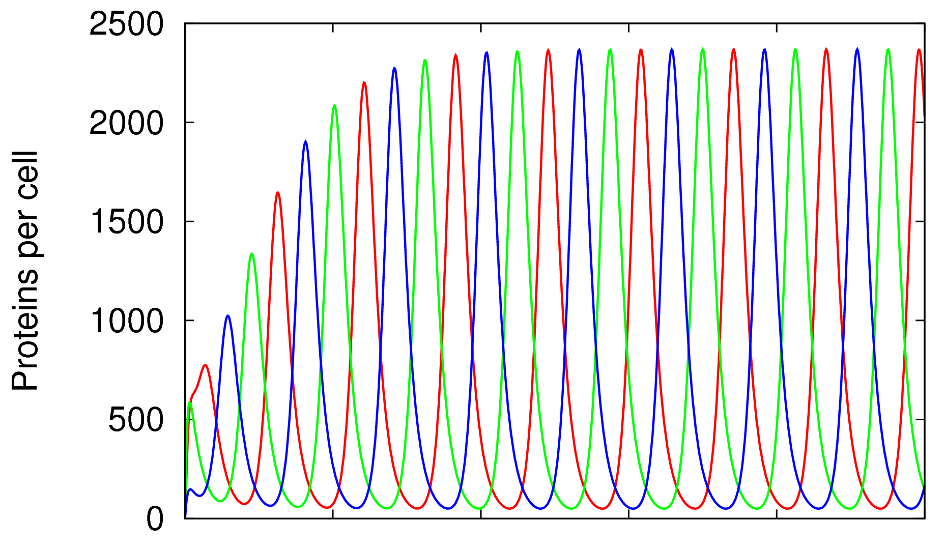
\includegraphics[width=0.6\textwidth]{images/simEx1.png}
\caption{Time-course simulation of the repressilator model, imported from BioModels Database and simulated in COPASI. The number of repressor proteins lacI, tetR and cI is shown. (taken from \cite{Waltemath:2011})}
\label{fig:simEx1}
\end{figure}

\subsection{Applying pre-processing}
\label{sec:examplePreprocessing}
The fine-tuning of the model can be shown by adjusting parameters before simulation. When changing the initial values of the parameters \emph{protein copies per promoter} and \emph{leakiness in protein copies per promoter} the system's behavior switches from sustained oscillation to asymptotic steady-state. The adjustments leading to that behavior may be described as: 

\begin{enumerate}
\item{Import the model as above.}
\item{Change the value of the parameter \code{tps$\_$repr} from “0.0005” to “1.3e-05”. }
\item{Change the value of the parameter \code{tps$\_$active} from “0.5 “ to “ 0.013“.}
\item{Select a deterministic method.}
\item{Run a uniform time course for the duration of 1000~min with an output interval of 1~min.}
\item Plot the amount of lacI, tetR and cI against time in a 2D Plot.
\end{enumerate}

\fig{simEx3} shows the result of the simulation.
%
\begin{figure}
\centering
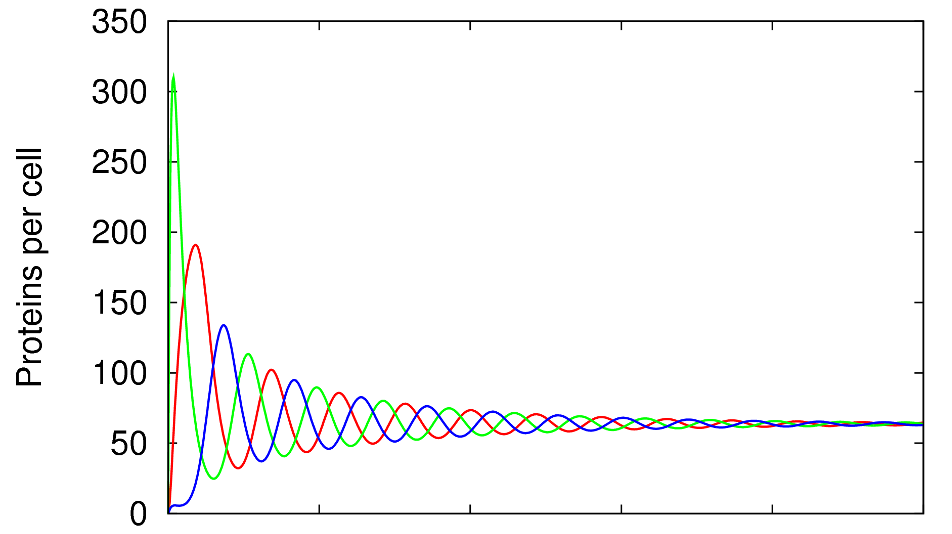
\includegraphics[width=0.7\textwidth]{images/simEx3.png}
\caption{Time-course simulation of the repressilator model, imported from BioModels Database and simulated in COPASI after modification of the initial values of the \emph{protein copies per promoter} and the \emph{leakiness in protein copies per promoter}. The number of repressor proteins lacI, tetR and cI is shown. (taken from \cite{Waltemath:2011})}
\label{fig:simEx3}
\end{figure}


\subsection{Applying post-processing}
The raw numerical output of the simulation steps may be subjected to data post-processing before plotting or reporting.  In order to describe the production of a normalized plot of the time-course in the first example (section \ref{sec:intro1}), depicting the influence of one variable on another (in phase-planes), one could define the following further steps:

(Please note that the description steps 1 - 4 remain as given in section \ref{sec:intro1} above.)
\begin{enumerate}
\item[5.]{Collect lacI(t) , tetR(t) and cI(t).}
\item[6.]{Compute the highest value for each of the repressor proteins,  max(lacI(t)), max(tetR(t)), max(cI(t)).}
\item[7.]{Normalize the data for each of the repressor proteins by dividing each time point by the maximum value, i.\,e.\ lacI(t)/max(lacI(t) ), tetR(t)/max(tetR(t)) , and cI(t)/max(cI(t)).}
\item[8.]{Plot the normalized \code{lacI} protein as a function of the normalized \code{cI}, the normalized \code{cI}  as a function of the normalized \code{tetR} protein, and the normalized \code{tetR} protein against the normalized \code{lacI} protein in a 2D plot.}
\end{enumerate}
\fig{simEx2} illustrates the result of the simulation after post-processing of the output data. 
\begin{figure}
\centering
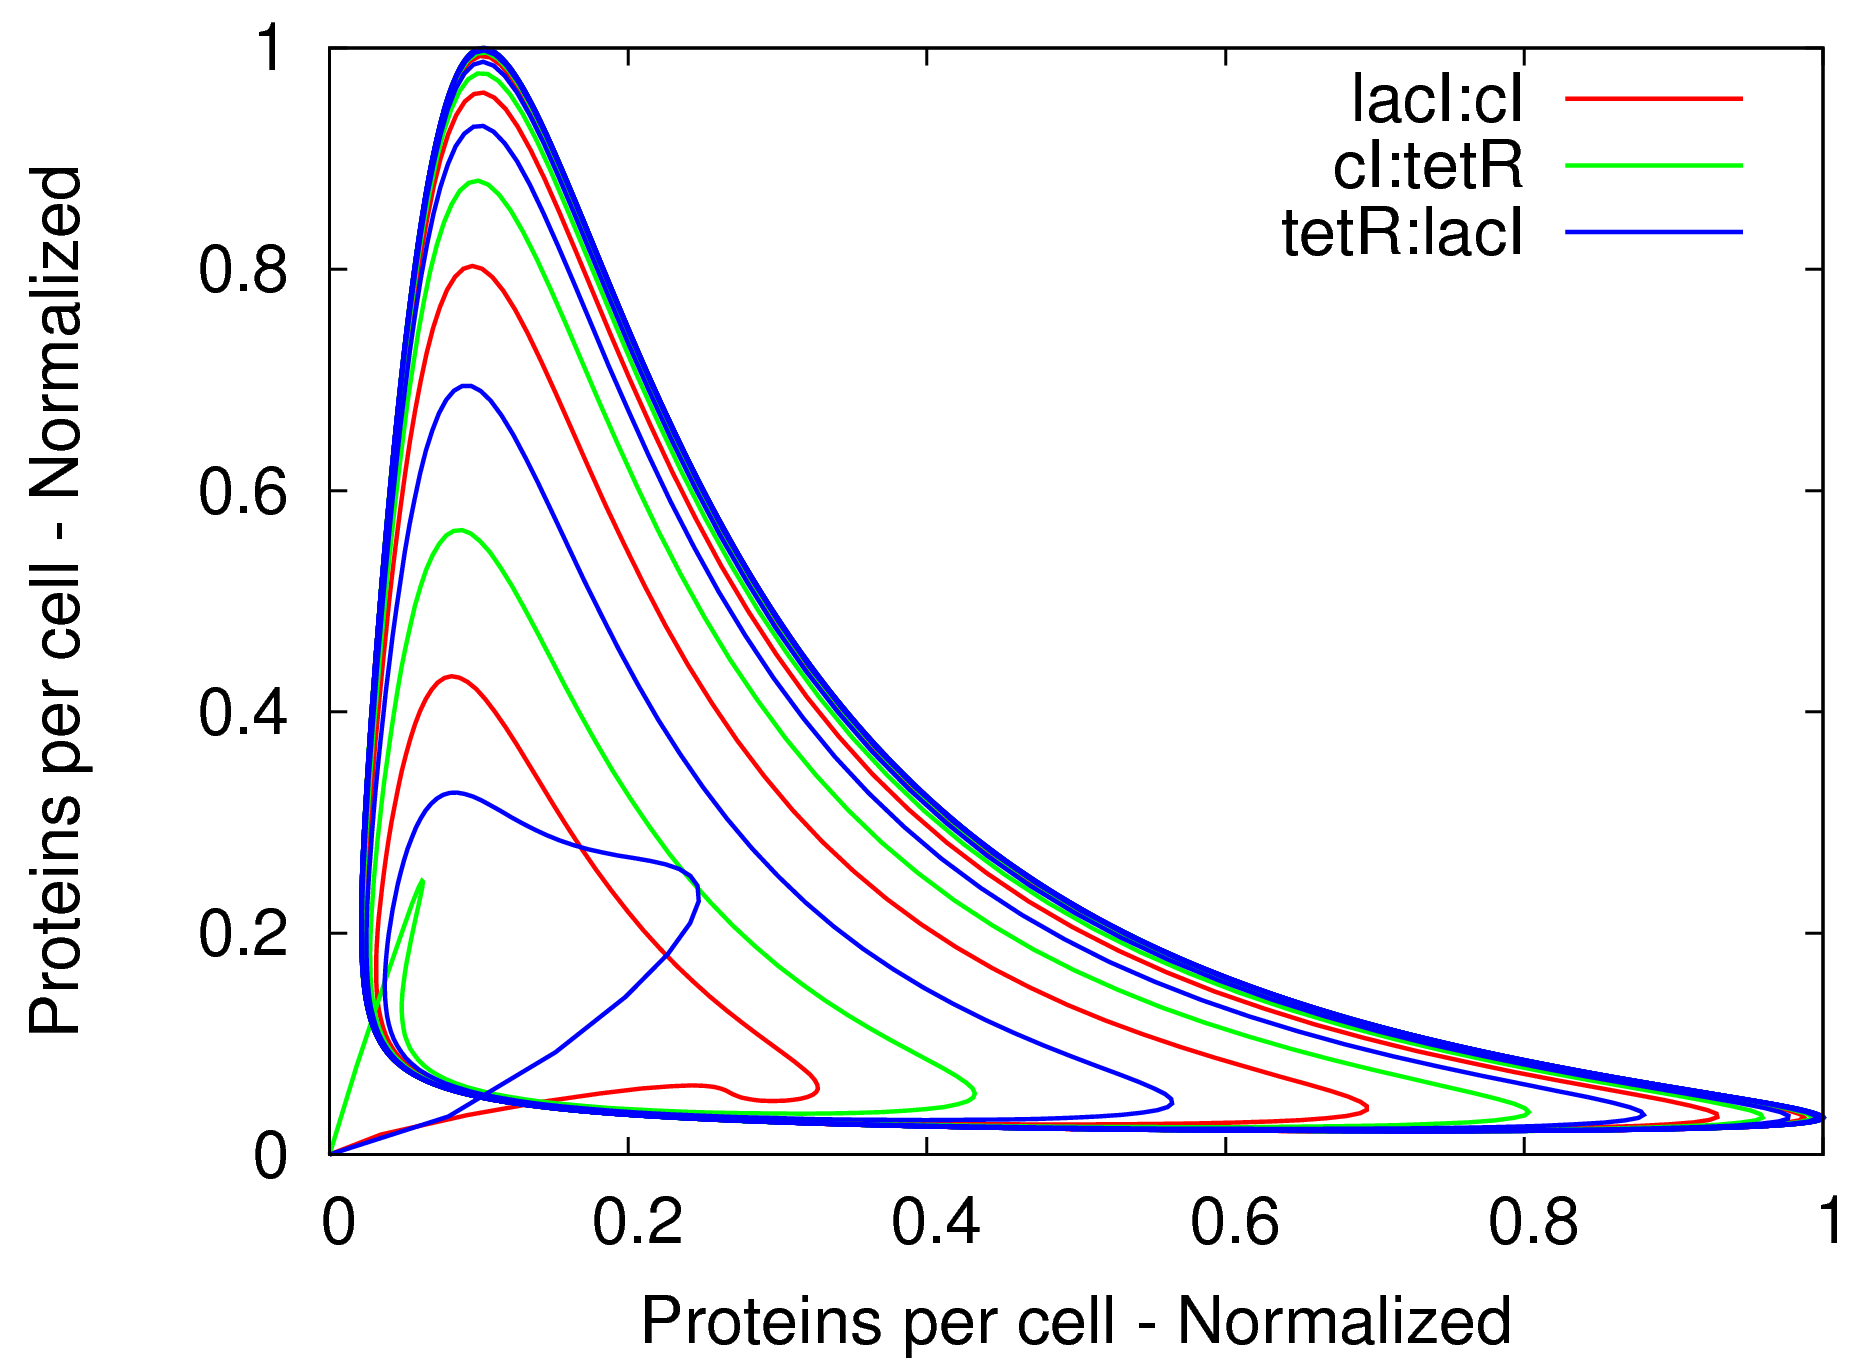
\includegraphics[width=0.7\textwidth]{images/simEx2.png}
\caption{Time-course simulation of the repressilator model, imported from BioModels Database and simulated in COPASI, showing the normalized temporal evolution of repressor proteins lacI, tetR and cI in phase-plane. (taken from \cite{Waltemath:2011})}
\label{fig:simEx2}
\end{figure}


%%% Local Variables: 
%%% mode: latex
%%% TeX-master: "../sed-ml-L1V3"
%%% End: 


% ~~~~~~~~~~~~~~~~~~~~~~~~~~~~~~~~~~~~
%% OVERVIEW  (BPMN)
% ~~~~~~~~~~~~~~~~~~~~~~~~~~~~~~~~~~~~
\chapter{Overview of SED-ML}
\label{sec:overview}
% overview
The \emph{Simulation Experiment Description Markup Language} (SED-ML) is an XML-based format for the description of simulation experiments. It serves to store information about the simulation experiment performed on one or more models with a given set of outputs. Support for SED-ML compliant simulation descriptions will enable the exchange of simulation experiments across tools.
\section{Conventions}
%
The Business Process Modeling Notation Version 1.2 (BPMN) was initially intended to describe internal business procedures (processes) in a graphical way. However, we will use BPMN to graphically describe the steps and processes of setting up a simulation experiment description. The major parts of BPMN that are used to specify SED-ML are activities, gateways, events, data, and documentation. 

An \emph{activity} is ``work that is performed on a [..] process'', for example ``Specify the simulation settings''. Activities may be atomic or non-atomic. SED-ML in particular makes use of the \emph{task} activities, \ie specific work units that need to be performed. Non-atomic tasks might be collapsed or expanded in the graphical representation (\fig{task}). Each collapsed subprocess has a corresponding expanded subprocess definition.

\begin{figure}[h]
\centering
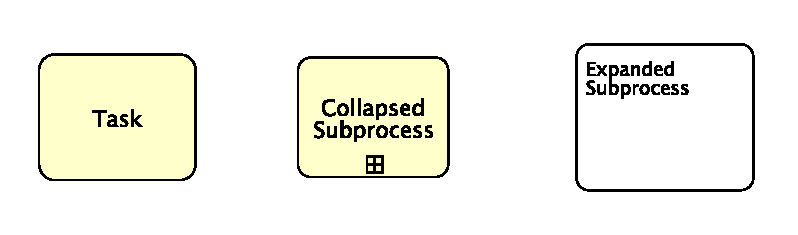
\includegraphics[width=0.5\textwidth]{images/processes.pdf}
\caption{BPMN activities: task, collapsed process, expanded subprocess}
\label{fig:task}
\end{figure}

\emph{Gateways} serve as means to control the flow of sequence in the diagram. As the term already implies, a gateway needs some ``mechanism that either allows or disallows passage through'' \citep{White:2004}. The result of a gateway pass-through can be that processes are merged or split. Graphically, a gateway is represented as a diamond. 

\begin{figure}[h]
\centering
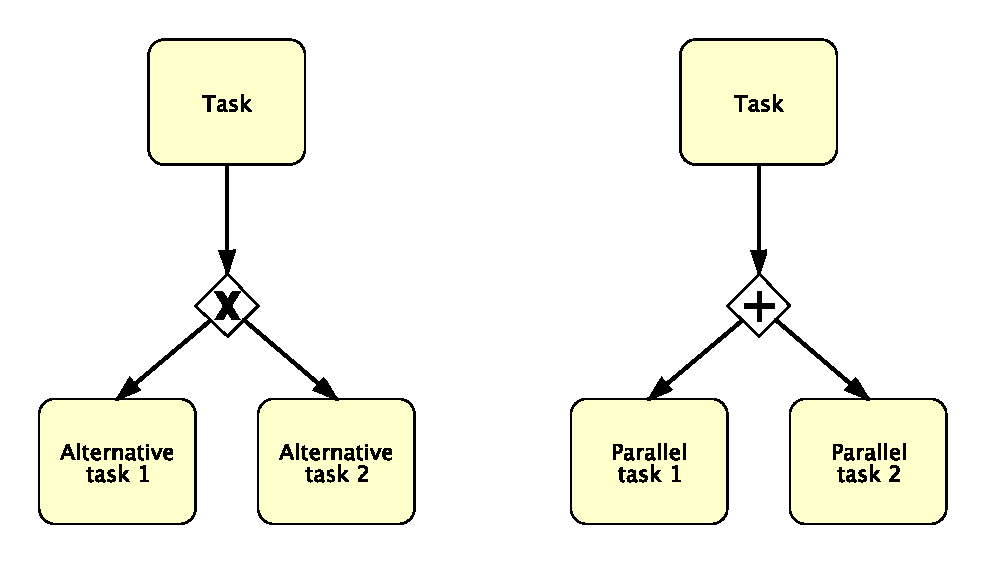
\includegraphics[width=0.5\textwidth]{images/gateways.pdf}
\caption{BPML gateway types: Exclusive (left), parallel (right)}
\label{fig:gateways}
\end{figure}

While there exist a number of different gateway types \citep[p.~93]{White:2004}, the SED-ML specification only uses the parallel and the exclusive gates  (\fig{gateways}). 

\emph{Exclusive} gateways -- also denoted as decisions -- allow the sequence flow to take two or more alternative paths (\fig{gateways}, left hand side). However, \emph{only one} of the paths may be chosen (not more). Sometimes two alternative branches need to be merged together again, in which case the exclusive gate must be used as well: The sequence flow continues as soon as \emph{one} of the incoming processes send a signal. An exclusive gateways is marked by an \code{X} in the graphical notation.

\emph{Parallel} gateways, ``provide a mechanism to synchronize parallel flow and to create parallel flow'' \citep{White:2004} (\fig{gateways}, right hand side). They are used to show parallel paths in the workflow; even if sometimes not required they might help in understanding the process. Synchronisation allows to start two processes in parallel at the same time in the sequence flow: The sequence flow will continue with \emph{all} processes leaving the parallel gateway. Joining two processes with a parallel gateway is also possible: the process flow will only continue after a signal has arrived from \emph{all} processes coming in the parallel gateway. A parallel gateway is marked by a \code{+} in the graphical notation.

\emph{Events} mark everything happening during the execution of the sequence flow, usually they interrrupt the business process, having some cause or impact on the execution. From the broad range of events that BPMN offers, SED-ML only uses a small subset, namely the start event and the end event (\fig{connectorEvents}).

\begin{figure}[h]
\centering
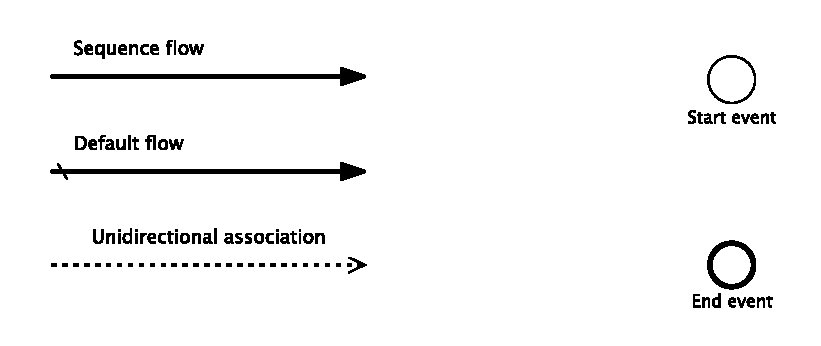
\includegraphics[width=0.5\textwidth]{images/connectors.pdf}
\caption{BPML connectors (left) and events (right).}
\label{fig:connectorEvents}
\end{figure}

All events are graphically drawn as small circles. A \emph{start event} is drawn with a single thin line and mark the start of a process, it can not have any incoming sequence flow. Start events may be triggered by different mechanisms, for the case of SED-ML the untyped start event (no marker inside the circle) is used. The trigger to start the process is ``Create new simulation experiment''. The \emph{end event} is marked with a thick line. It indicates the end of a process. SED-ML specification makes use of the untyped end event (no marker inside the circle). The end event is used to show the end of sub-processes as well as processes. If the end of a sub-process is reached, the sequence flow returns to the according parent process.

\emph{Connectors} are used to combine different BPMN objects with each other (\citet[p.~30]{White:2004} show the full list of valid connections). SED-ML uses only a subset of available connectors, namely sequence flow, default flow, and unidirectional associations (\fig{connectorEvents}). \emph{Sequence flow} defines the execution order of activities. \emph{Default flow} marks the default branch to be chosen if other conditions leave various possibilities for further execution of the sequence flow. A \emph{unidirectional association} is used to indicate that a data object is modified, i.\,e. read and written during the execution of an activity \citep{bpmnPoster}.

%
The rough SED-ML workflow is shown in Figure \ref{fig:sedmlWorkflow}.
%
\begin{figure}[h]
\centering
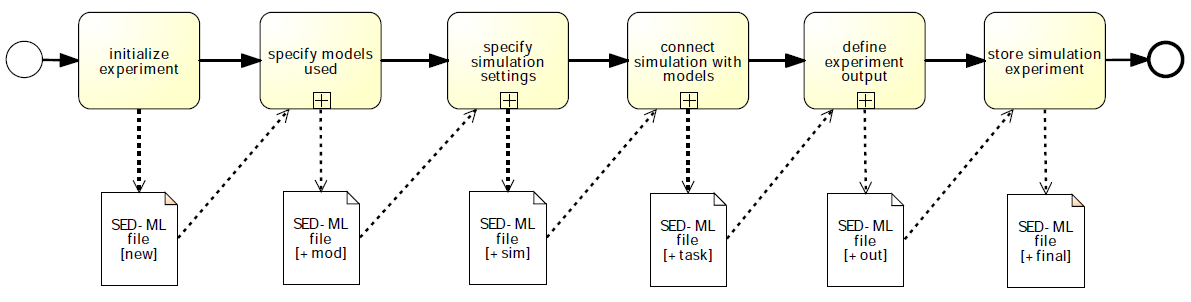
\includegraphics[width=\textwidth]{images/bpmn/sedMainOryx.png}
\caption{The process of defining a simulation experiment in SED-ML (overview)}
\label{fig:sedmlWorkflow}
\end{figure}
%
The process of defining a SED-ML simulation experiment starts by initialising the experiment and creating a new SED-ML file. Afterwards, the \concept{models} needed for the simulation are specified and stored into the existing SED-ML file (Section~\ref{overview:models}). In a third step, the simulation experiment \concept{setups} are defined and stored into the same file (Section~\ref{overview:simulation}). To assign a setup to a number of models used in the experiment, these connections have to be defined and recorded (Section~\ref{overview:task}), called \concept{task} in SED-ML. After simulation, the \concept{output} should be defined, based on the specified tasks and performed simulation experiment. The information is added to the existing SED-ML file (Section~\ref{overview:output}). In the end, the whole experiment is stored in the final SED-ML file.
%
All collapsed processes are described in the following sections. Examples in XML are provided in the more technical description.

\section{Models}
\label{overview:models}
To define a simulation experiment, first of all a new SED-ML file is created. The models to be used in the experiment (zero or many) are referenced, using a link to a model description in some open, curated model database (e.\,g.\ Biomodels Database \citep{LDR+10} or CellML Repository \citep{BBC+09}). All necessary changes to correctly simulate the model are defined, e.\,g., assigning new parameter values or updating the mathematics of the model (Figure~\ref{fig:workflowModel}).
%
\begin{figure}[h]
\centering
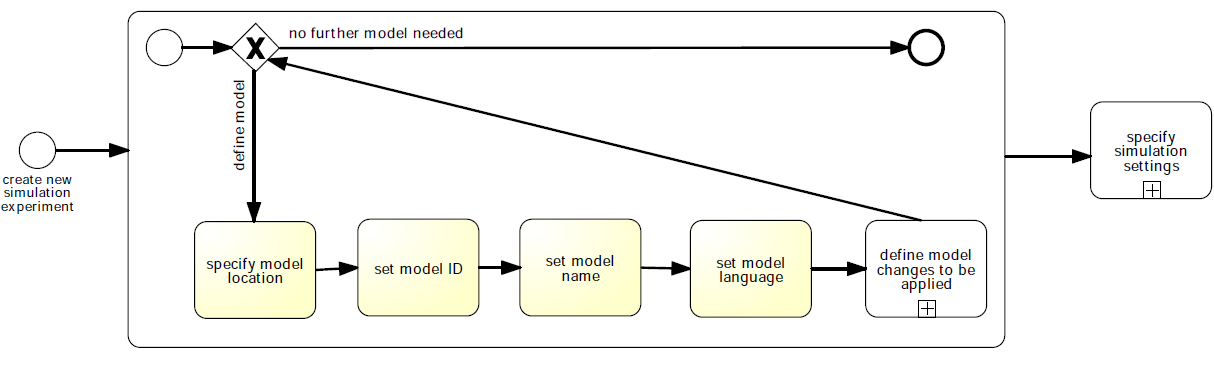
\includegraphics[width=0.8\textwidth]{images/bpmn/sedModelOryx.png}
\caption{The process of defining model(s) in SED-ML}
\label{fig:workflowModel}
\end{figure}
%
The procedure is repeated until all models participating in the experiment have been described. Each such model gets an internal SED-ML ID and an optional name.

\section{Simulation setup}
\label{overview:simulation}
Secondly, the simulation setups (zero or many) used throughout the simulation experiment are described (Figure \ref{fig:workflowSimulation}). 
%
%
\begin{figure}[h]
\centering
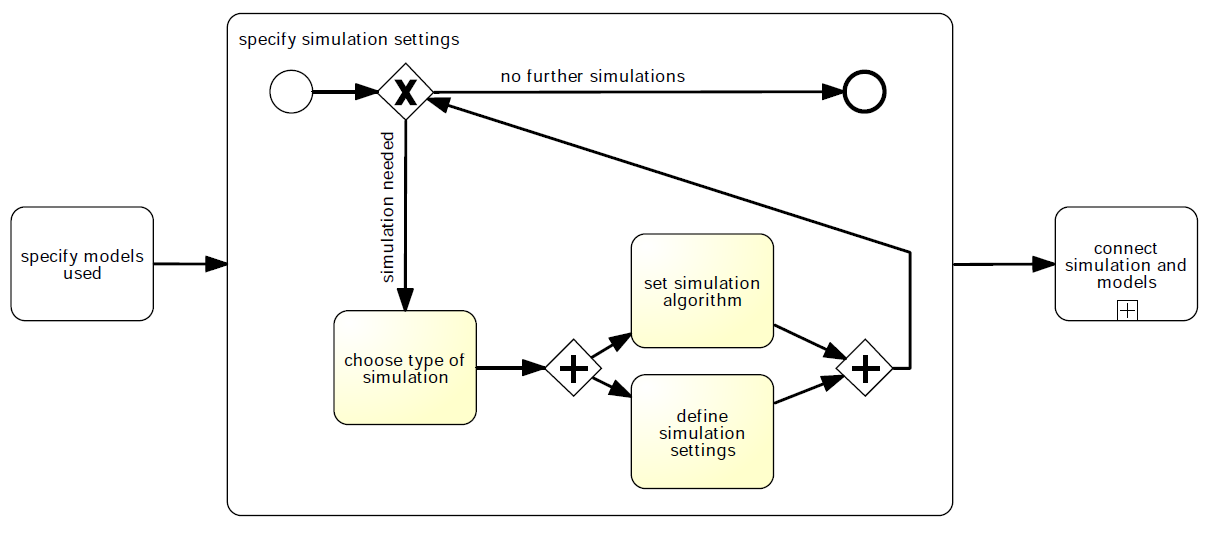
\includegraphics[width=0.8\textwidth]{images/bpmn/sedSimulationOryx.png}
\caption{The process of defining simulation(s) in SED-ML}
\label{fig:workflowSimulation}
\end{figure}
%
Those may stem from various different types of simulation, e.\,g., steady state analysis or bifurcation.  Depending on the specific type of experiment, the information encoded for the simulation setup might differ. Thus, the definition of simulation settings is specific to the simulation experiment.

In a simple case the experiment consists of one simulation, but it can get far more complex. For example, one might define a nested sequence of simulations, in which case every simulation has to be defined separately.
Each simulation setup gets its own internal ID and an optional name. For each of the setups, the simulation algorithm to be used for that simulation is defined through a reference to a well-defined algorithm name, e.\,g. an ontology or controlled vocabulary. One approach to define such a controlled vocabulary of simulation algorihtms is the \emph{Kinetic Simulation Algorithm Ontology} (Section~\ref{sec:kisao}). 
%
The setup definition is repeated until all different simulations have been described.

\section{Task}
\label{overview:task}
SED-ML allows to apply one defined simulation setting to one defined model at a time. However, any number of \concept{tasks} may be defined inside a simulation experiment description (Figure \ref{fig:workflowTask}). 
%
\begin{figure}[h]
\centering
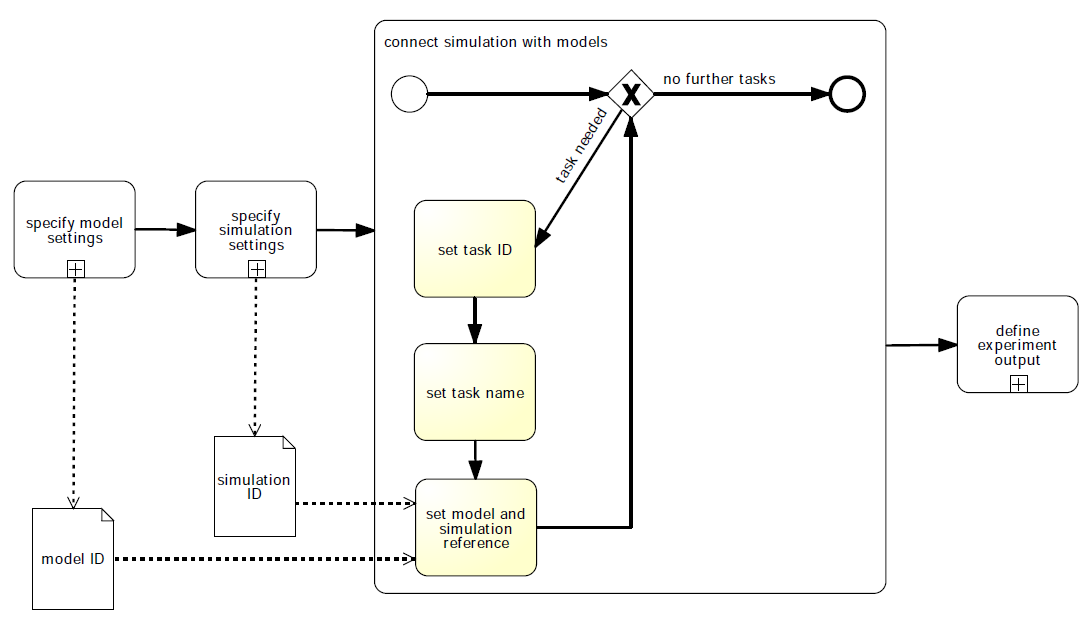
\includegraphics[width=0.7\textwidth]{images/bpmn/sedTaskOryx.png}
\caption{The process of defining simulation task(s) in SED-ML}
\label{fig:workflowTask}
\end{figure}
%
To do so, each task refers to one of the formerly specified models and to one of the formerly specified simulation setups. Each task has its own ID and an optional name. The process of task definition is repeated until all tasks have been defined.


\section{Output}
\label{overview:output}
The SED-ML finally consists of output definitions that describe what kind of output the experiment uses to present the simulation result to the user, i.\,e., a plot or a data table (Figure \ref{fig:workflowOutput}), and also which data is part of the output. 
%
\begin{figure}[h]
\centering
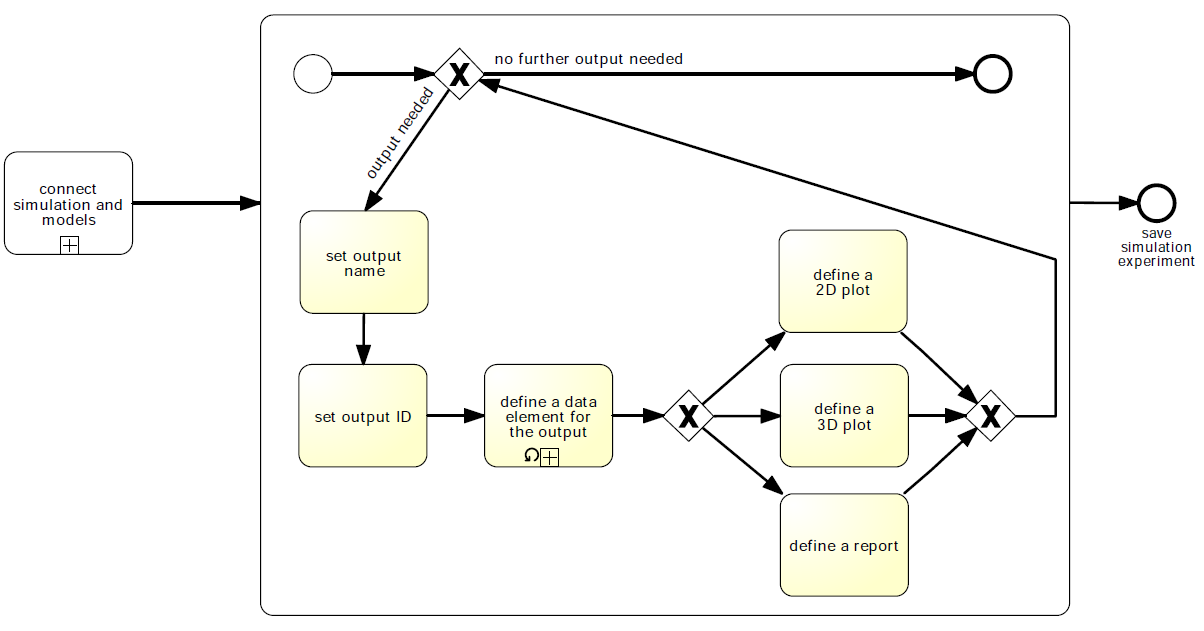
\includegraphics[width=0.7\textwidth]{images/bpmn/sedOutputOryx.png}
\caption{The process of defining output(s) in SED-ML}
\label{fig:workflowOutput}
\end{figure}
%
Therefore, SED-ML first defines a set of \concept{data generators} (Figure \ref{fig:workflowDataGenerator}), which are then used to specify a particular result, i.\,e. output (Section~\ref{overview:dataGen}). 

The SED-ML specification comes with three pre-defined types of outputs: 2D- and 3D plots, and reports. All use the aforementioned data generators to specify the information to be plotted on the different axes, or in the table comlumns respectively.
\section{Data Generator}
\label{overview:dataGen}
%
\begin{figure}[h]
\centering
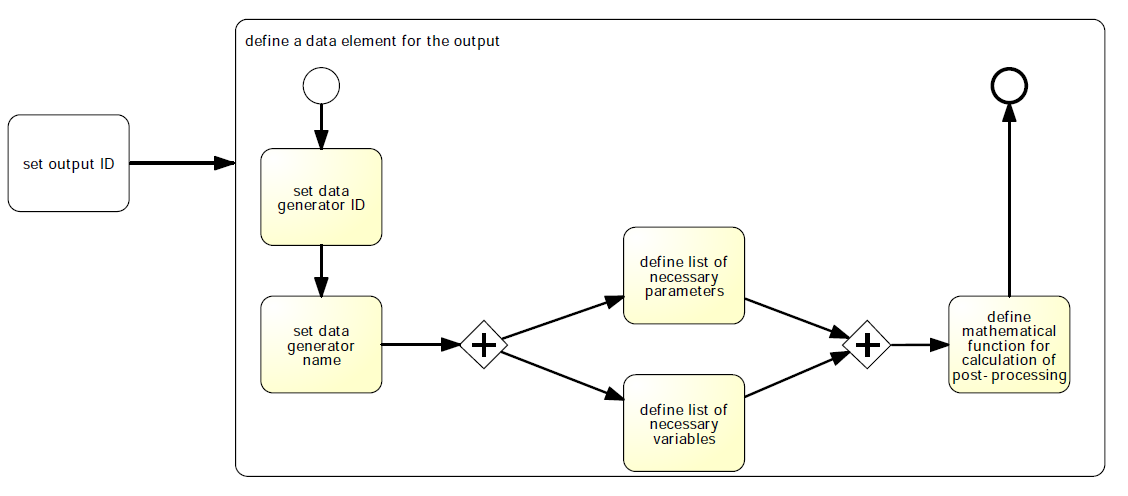
\includegraphics[width=0.7\textwidth]{images/bpmn/sedDataGeneratorOryx.png}
\caption{The process of defining data generator(s) in SED-ML}
\label{fig:workflowDataGenerator}
\end{figure}
%
A data generator may use data elements, e.\,g., variables or parameters, that either (1) have been taken directly from the model, or (2) have been generated in a post-processing step. If post-processing needs to be applied, variables and parameters from the various, previously defined models may be used, but also existing global parameters, such as \emph{time}.
If the variables are taken from existing models, a reference to the model and the particular variable needs to be given. 
If post-processing is necessary, a reference to an existing variable or parameter, including other data generators, has to be provided. Additional mathematical rules to be applied on the referred variable or parameter must then  be specified. 
%
In a SED-ML file, any number of data generators can be created for later re-use in the output definition.



%%% Local Variables: 
%%% mode: latex
%%% TeX-master: "../sed-ml-L1V2"
%%% End: 



%%% Local Variables: 
%%% mode: latex
%%% TeX-master: "../sed-ml-L1V2"
%%% End: 


% ~~~~~~~~~~~~~~~~~~~~~~~~~~~~~~~~~~~~~~~~
%% TECHNICAL SPECIFICATION
% ~~~~~~~~~~~~~~~~~~~~~~~~~~~~~~~~~~~~~~~~
\chapter{SED-ML technical specification}
\label{chp:specification}
This document represents the technical specification of SED-ML \currentLV. The corresponding UML class diagram is shown in \fig{sedML}. Example simulation experiments in SED-ML are provided in Appendix~\ref{app:examples}. The XML Schema is provided in Appendix~\ref{app:schema}. However, not all concepts of SED-ML can be captured using XML Schema alone. In such cases this specification is the normative document. 

\sedfig[width=\textwidth]{images/uml/all}{The SED-ML \currentLV UML class diagram}{fig:sedML}

\settocdepth{subsubsection}

%% ~~~ GENERAL LANGUAGE ELEMENTS ~~~
\pagebreak

\section{General attributes and classes}
In this section we introduce attributes and concepts used repeatedly throughout the SED-ML specification. 


% ~~~~~~~~~~~~~~~~~~~~~~~~~~~~~~~~~~~~
% PRIMITIVE DATA TYPES
% ~~~~~~~~~~~~~~~~~~~~~~~~~~~~~~~~~~~~
\subsection{Primitive data types}
Most primitive types in SED-ML are taken from the data types defined in XML Schema 1.0, including \code{string}, \code{boolean}, \code{int}, \code{positiveInteger} and \code{double}. A few other primitive types are defined by SED-ML itself: 

\subsubsection{Type ID}
\label{type:id}
The XML Schema 1.0 type ID is identical to the XML 1.0 type ID. The literal representation of this type consists of strings of characters restricted as summarized in Figure~\vref{fig:id}. For a detailed description see the SBML specification on the type \code{ID} \citep{HBH+10}.

\begin{figure}[hbt]
  \ttfamily
  \small
  \centering
  \begin{tabular}{lll}
    NameChar & ::= & letter | digit | '.' | '-' | ' ' | ':' | CombiningChar | Extender\\
    ID    & ::= & ( letter | ' ' | ':' ) NameChar*\\
  \end{tabular}
  \vspace*{-1ex}
  \caption{The definition of the type \code{ID}. The characters ( and ) are used for grouping, the character * indicates "zero or more times", and the character | indicates "or". Please consult the XML 1.0 specification for the complete definitions of letter, digit, CombiningChar, and Extender.}
  \label{fig:id}
\end{figure}

\subsubsection{Type SId}
\label{type:sid}
The type \code{SId} is the type of the id attribute found on the majority of SED-ML coponents. \code{SId} is a datatype derived from the basic XML type \code{string}, but with restrictions about the characters permitted and the sequences in which those characters may appear. The definition is shown in Figure~\vref{fig:sid}. For a detailed description see the SBML specification on the type \code{SId} \citep{HBH+10}.

\begin{figure}[hbt]
  \ttfamily
  \small
  \centering
  \begin{tabular}{lll}
    letter & ::= & 'a'..'z','A'..'Z'\\
    digit  & ::= & '0'..'9'\\
    idChar & ::= & letter | digit | '\_'\\
    SId    & ::= & ( letter | '\_' ) idChar*\\
  \end{tabular}
  \vspace*{-1ex}
  \caption{The definition of the type \code{SId}}
  \label{fig:sid}
\end{figure}


\subsubsection{Type SIdRef}
\label{type:sidref}
Type \code{SIdRef} is used for all attributes that refer to identifiers of type \code{SId} in a model. This type is derived from \code{\hyperref[type:sid]{SId}}, but with the restriction that the value of an attribute having type \code{SIdRef} must equal the value of some \code{SId} attribute in the model where it appears. In other words, a \code{SIdRef} value must be an existing idetifier in a model. 

As with \code{SId}, the equality of SIdRef values is determined by exact character sequence match; i.e., comparisons of these identifiers must be performed in a case-sensitive manner.

\subsubsection{Type XPath}
\label{type:xpath}
Type \code{XPath} is used to identify nodes and attributes within an XML representation of a biological model. \code{XPath} is hereby a XPath version 1 expression which can be used to unambiguously identify an element or attribute in an XML file.

\subsubsection{Type MathML}
\label{type:mathml}
Type \code{MathML} is used to describe mathematical expression. For a description of the allowed subset of \code{MathML} see Section~\ref{sec:mathML}.

\subsubsection{Type anyURI}
\label{type:anyURI}
Type \code{anyURI} is used to reference models, reference data files, specify the language of referenced models, for referencing implicit model variables and in annotations. For a description of the uses of \code{anyURI} see Section~\ref{sec:uriScheme}.

\subsubsection{Type NuMLSIdRef}
\label{type:numlsidref}
\hl{TODO: explain, probably also NuMLSId}


% ~~~~~~~~~~~~~~~~~~~~~~~~~~~~~~~~~~~~
% ID
% ~~~~~~~~~~~~~~~~~~~~~~~~~~~~~~~~~~~~
\subsection{\element{id}}
\label{sec:id}
Most objects in SED-ML carry an \concept{id} attribute of data type \code{\hyperref[type:sid]{SId}}. The \hyperref[sec:id]{id} attribute, if it exists for an object, is required and identifies SED-ML constituents unambiguously. All \code{id}s have a global scope, i.\,e.\ the \code{id} must be unambiguous throughout a whole SED-ML document.

An example for a defined \concept{id} is given in Listing~\ref{lst:id}.

\begin{myXmlLst}{SED-ML identifier definition, e.\,g.\ for a model}{lst:id}
<model id="m00001" language="urn:sedml:language:sbml" source="urn:miriam:biomodels.db:BIOMD0000000012">
	[MODEL DEFINITION]
</model>
\end{myXmlLst}

The defined model carries the  \code{id} \code{m00001}. If the model is referenced elsewhere in the SED-ML document, it is referred to by that \code{id}.


% ~~~~~~~~~~~~~~~~~~~~~~~~~~~~~~~~~~~~
% NAME
% ~~~~~~~~~~~~~~~~~~~~~~~~~~~~~~~~~~~~
\subsection{\element{name}}
\label{sec:name}
SED-ML constituent may have an optional \concept{name} of data type \code{String}. Names do not have identifying character, i.\,e.\ several SED-ML constituents may carry the same name. The purpose of the \code{name} attribute is to keep a human-readable name of the constituent, e.\,g.\ for display to the user.

Listing \ref{lst:name} extends the model definition in \lst{id} by a model name.

\begin{myXmlLst}{SED-ML name definition, e.\,g.\ for a model}{lst:name}
<model id="m00001" name="Circadian oscillator" language="urn:sedml:language:sbml" source="urn:miriam:biomodels.db:BIOMD0000000012">
	[MODEL DEFINITION]
</model>
\end{myXmlLst}


% ~~~~~~~~~~~~~~~~~~~~~~~~~~~~~~~~~~~~
% SEDBASE
% ~~~~~~~~~~~~~~~~~~~~~~~~~~~~~~~~~~~~
\subsection{\element{SEDBase}}
\label{class:sedBase}
\concept{SEDBase} is the base class of SED-ML \currentLV. All other classes are derived from it. As such it provides means to attach additional information on all other classes (\fig{sedBase}). That information can be specified by human readable \hyperref[class:notes]{Notes} or custom \hyperref[class:annotation]{Annotations}.

\sedfig[width=0.7\textwidth]{images/uml/sedBase}{The SEDBase class}{fig:sedBase}

\tabtext{sedbase}{SEDBase}
\begin{table}[ht]
\center
\begin{tabular}{ll}

\toprule
\textbf{\attribute} & \textbf{\desc}\\
\midrule
metaid$^{o}$ & \refpage{sec:metaID} \\
\midrule
\textbf{\subelements} & \textbf{\desc}\\
\midrule
notes$^{o}$ & \refpage{class:notes}\\
annotation$^{o}$ & \refpage{class:annotation}\\
\bottomrule
\end{tabular}
\caption{\tabcap{SEDBase}}
\label{tab:sedbase}
\end{table}


% ~~~~~~~~~~~~~~~~~~~~~~~~~~~~~~~~~~~~
% META ID
% ~~~~~~~~~~~~~~~~~~~~~~~~~~~~~~~~~~~~
\subsubsection{\element{metaid}}
\label{sec:metaID}
The main purpose of the \element{metaid} attribute of data type \code{\hyperref[type:id]{ID}} is to attach semantic annotations in form of the \hyperref[class:annotation]{Annotation} class to SED-ML elements. The \code{metaid} attribute is globally unique throughout the SED-ML document, i.\,e.\ the \code{metaid} must be unambiguous throughout a whole SED-ML document. As such it identifies the constituent it is related to.

An example showing how to link a semantic annotation to a SED-ML object via the \element{metaid} is given in the \hyperref[class:annotation]{Annotation} class description.


% ~~~~~~~~~~~~~~~~~~~~~~~~~~~~~~~~~~~~
% NOTES
% ~~~~~~~~~~~~~~~~~~~~~~~~~~~~~~~~~~~~
\subsubsection{\element{Notes}}
\label{class:notes}
A \concept{note} is considered a human-readable description of the element it is assigned to. It serves to display information to the user. Instances of the \concept{Notes} class may contain any valid XHTML \citep{P+02}, ranging from short comments to whole HTML pages for display in a Web browser. The namespace URL for \code{XHTML} content inside the \hyperref[class:notes]{Notes} class is \url{http://www.w3.org/1999/xhtml}. It may either be declared in the \hyperref[class:sed-ml]{\code{sedML} XML element}, or directly used in top level XHTML elements contained within the  \code{notes} element. For further options of how to set the namespace and detailed examples, please refer to \citep[p. 14]{HBH+10}.

\tabtext{notes}{Notes}

\begin{table}[ht]
\center
\begin{tabular}{ll}
\toprule
\textbf{\attribute} & \textbf{\desc}\\
\midrule
xmlns:string & \refpage{sec:xmlns} \\
 {``http://www.w3.org/1999/xhtml" } & \\
\midrule
\textbf{\subelements} & \textbf{ }\\
\midrule
\emph{well-formed content permitted in XHTML} & \\
\bottomrule
\end{tabular}
\caption{\tabcap{Notes}}
\label{tab:notes}
\end{table}

\code{Notes} does not have any further sub-elements defined in SED-ML, nor attributes associated with it.

\lsttext{notes}{notes}

\begin{myXmlLst}{The \element{notes} element}{lst:notes}
<sedML [..]>
	<notes >
  		<p xmlns="http://www.w3.org/1999/xhtml">The enclosed simulation description shows the oscillating behaviour of the Repressilator model using deterministic and stochastic simulators.</p>
	</notes>
</sedML>
\end{myXmlLst}

In this example, the namespace declaration is inside the \element{notes} element and the note is related to the \element{sedML} root element of the SED-ML file. A note may, however, occur inside \emph{any} SED-ML XML element, except \code{note} itself and \hyperref[class:annotation]{\code{annotation}}.


% ~~~~~~~~~~~~~~~~~~~~~~~~~~~~~~~~~~~~
% ANNOTATION
% ~~~~~~~~~~~~~~~~~~~~~~~~~~~~~~~~~~~~
\subsubsection{\element{Annotation}}
\label{class:annotation}

An \concept{annotation} is considered a computer-processible piece of information. Annotations may contain any valid XML content. For further guidelines on how to use annotations, we would like to encourage the reading of the corresponding section in the SBML specification \citep[pp. 14-16]{HBH+10}. The style of annotations in SED-ML is briefly described in Section~\ref{sec:annotations} on page \pageref{sec:annotations}.

\tabtext{annotation}{Annotation}

\begin{table}[ht]
\center
\begin{tabular}{ll}
\toprule
\textbf{\attribute} & \textbf{\desc}\\
\midrule
\emph{none} & \\
\midrule
\textbf{\subelements} & \textbf{\desc}\\
\midrule
\emph{none in the SED-ML namespace} & \\
\bottomrule
\end{tabular}
\caption{\tabcap{Annotation}}
\label{tab:annotation}
\end{table}

\lsttext{annotation}{annotation}

\begin{myXmlLst}{The annotation element}{lst:annotation}
<sedML>
	[..]
	<model id="model1" metaid="_001" language="urn:sedml:language:cellml" source="http://models.cellml.org/workspace/leloup_gonze_goldbeter_1999/@@rawfile/d6613d7e1051b3eff2bb1d3d419a445bb8c754ad/leloup_gonze_goldbeter_1999_a.cellml" >
		<annotation>
    		<rdf:RDF xmlns:rdf="http://www.w3.org/1999/02/22-rdf-syntax-ns#" xmlns:bqmodel="http://biomodels.net/model-qualifiers/">
				<rdf:Description rdf:about="#_001">
				<bqmodel:isDescribedBy>
				<rdf:Bag>
					<rdf:li rdf:resource="urn:miriam:pubmed:10415827"/>
				</rdf:Bag>
				</bqmodel:isDescribedBy>
    			</rdf:Description>
			</rdf:RDF>
		</annotation>
	</model>
	[..]
</sedML>
\end{myXmlLst}

In that example, a SED-ML \hyperref[class:model]{model} element is annotated with a reference to the original publication. The \element{model} contains an \element{annotation} that uses the \concept{biomodels.net model-qualifier} \element{isDescribedBy} to link to the external resource \element{urn:miriam:pubmed:10415827}. In natural language the annotation content could be interpreted as ``The model is described by the published article available from pubmed under ID 10643740''. The example annotation follows the proposed \hyperref[sec:uriScheme]{URI Scheme} suggested by the MIRIAM reference standard. The MIRIAM URN can be resolved to the PubMED publication with ID 10415827, namely the article ``Alternating oscillations and chaos in a model of two coupled biochemical oscillators driving successive phases of the cell cycle.'' published by Romond et al. in  1999.


% ~~~~~~~~~~~~~~~~~~~~~~~~~~~~~~~~~~~~
% SED-ML
% ~~~~~~~~~~~~~~~~~~~~~~~~~~~~~~~~~~~~
\subsection{\element{SED-ML} top level element}
\label{class:sed-ml}
Each SED-ML \currentLV document has a main class called SED-ML which defines the document's structure and content (\fig{sed-mlMain}).

It consists of several parts; the parts are all connected to the SED-ML class through aggregation: 
\begin{itemize}
	\item the \hyperref[class:dataDescription]{DataDescription} class (for resolving external data, see Section~\ref{class:dataDescription}), 
	\item the \hyperref[class:model]{Model} class (for model specification, see Section~\ref{class:model}), 
	\item the \hyperref[class:simulation]{Simulation} class (for simulation setup specification, see Section~\ref{class:simulation}), 
	\item the \hyperref[class:abstractTask]{AbstractTask} class (for the linkage of models and simulation setups, see Section~\ref{class:abstractTask}), 
	\item the \hyperref[class:dataGenerator]{DataGenerator} class (for the definition of post-processing, see Section~\ref{class:dataGenerator}),
	\item and the \hyperref[class:output]{Output} class (for the output specification, see Section~\ref{class:output}).
\end{itemize}

All of them are shown in \fig{sed-mlMain} and will be explained in more detail in the relevant sections of this document.

\sedfig[width=0.8\textwidth]{images/uml/sed-ml}{The SED-ML class}{fig:sed-mlMain}

\tabtext{sed-ml}{SED-ML}

\begin{table}[ht]
\center
\begin{tabular}{ll}
\toprule
\textbf{\attribute} & \textbf{\desc}\\
\midrule
metaid$^{o}$ & \refpage{sec:metaID}\\
xmlns & \refpage{sec:xmlns}\\
level & \refpage{sec:level}\\
version & \refpage{sec:version}\\
\midrule
\textbf{\subelements} & \textbf{\desc}\\
\midrule
notes$^{o}$ & \refpage{class:notes}\\
annotation$^{o}$ & \refpage{class:annotation}\\
listOfDataDescriptions$^{o}$ & \refpage{sec:listOfDataDescriptions}\\
listOfModels$^{o}$ & \refpage{sec:listOfModels}\\
listOfSimulations$^{o}$ & \refpage{sec:listOfSimulations} \\
listOfTasks$^{o}$ & \refpage{sec:listOfTasks} \\
listOfDataGenerators$^{o}$ & \refpage{sec:listOfDataGenerators} \\
listOfOutputs$^{o}$ & \refpage{sec:listOfOutputs} \\
\bottomrule
\end{tabular}
\caption{\tabcap{SED-ML}}
\label{tab:sed-ml}
\end{table}

A SED-ML document needs to have the SED-ML namespace defined through the mandatory \hyperref[sec:xmlns]{xmlns} attribute. In addition, the SED-ML \hyperref[sec:level]{level} and \hyperref[sec:version]{version} attributes are mandatory.

The basic XML structure of a SED-ML file is shown in listing  \vref{lst:sedmlRoot}.

\begin{myXmlLst}{The SED-ML root element}{lst:sedmlRoot}
<?xml version="1.0" encoding="utf-8"?>
<sedML xmlns:math="http://www.w3.org/1998/Math/MathML" 
       xmlns="http://sed-ml.org/sed-ml/level1/version3" level="1" version="3">
	<listOfDataDescriptions>
	  	[DATA REFERENCES AND TRANSFORMATIONS]
  	</listOfDataDescriptions>
	<listOfModels>
		[MODEL REFERENCES AND APPLIED CHANGES]	 	
 	</listOfModels>
	<listOfSimulations>
		[SIMULATION SETUPS]
	</listOfSimulations>
	<listOfTasks>
		[MODELS LINKED TO SIMULATIONS]
	</listOfTasks>
	<listOfDataGenerators>
		[DEFINITION OF POST-PROCESSING]
	</listOfDataGenerators>
	<listOfOutputs>
		[DEFINITION OF OUTPUT]
	</listOfOutputs>
</sedML>
\end{myXmlLst}

The root element of each SED-ML XML file is the \code{sedML} element, encoding \hyperref[sec:version]{version} and \hyperref[sec:level]{level} of the file, and setting the necessary namespaces. Nested inside the \code{sedML} element are the six lists serving as containers for the encoded data (\concept{listOfDataDescriptions} for all external data sources, \concept{listOfModels} for all models, \concept{listOfSimulations} for all simulations, \concept{listOfTasks} for all tasks, \concept{listOfDataGenerators} for all post-processing definitions, and \concept{listOfOutputs} for all output definitions).

% ~~~ XMLNS ~~~
\subsubsection{\element{xmlns}}
\label{sec:xmlns}
The \concept{xmlns} attribute declares the namespace for the SED-ML document. The pre-defined namespace for SED-ML documents is \url{http://sed-ml.org/sed-ml/level1/version3}. 

In addition, SED-ML makes use of the \concept{MathML} namespace \url{http://www.w3.org/1998/Math/MathML} to enable the encoding of mathematical expressions in MathML 2.0. SED-ML uses a subset of MathML as described in Section~\ref{sec:mathML} on page \pageref{sec:mathML}.

SED-ML \concept{notes} use the XHTML namespace \url{http://www.w3.org/1999/xhtml}.  The \hyperref[class:notes]{Notes} class is described in Section~\ref{class:notes} on page \pageref{class:notes}.

Additional external namespaces might be used in \hyperref[class:annotation]{annotations}. 

% ~~~ LEVEL ~~~
\subsubsection{\element{level}}
\label{sec:level}
The current SED-ML \concept{level} is ``level \level''. Major revisions containing substantial changes will lead to the definition of forthcoming levels.

The level attribute is \code{required} and its value is a \code{fixed} decimal. For SED-ML \currentLV the value is set to \code{1}, as shown in the example in Listing~\ref{lst:sedmlRoot}.

% ~~~ VERSION ~~~
\subsubsection{\element{version}}
\label{sec:version}
The current SED-ML \concept{version} is ``version \version''. Minor revisions containing corrections and refinements of SED-ML elements, or new constructs which do not affect backwards compatibility, will lead to the definition of forthcoming versions.

The version attribute is \code{required} and its value is a \code{fixed} decimal. For SED-ML \currentLV the value is set to \code{\version}, as shown in the example in Listing~\ref{lst:sedmlRoot}.


% ~~~~~~~~~~~~~~~~~~~~~~~~~~~~~~~~~~~~
% REFERENCE RELATION
% ~~~~~~~~~~~~~~~~~~~~~~~~~~~~~~~~~~~~
\subsection{Reference relations}
\label{sec:reference}

The \concept{reference} concept is used to refer to a particular element inside the SED-ML document. It may occur in different ways in the SED-ML document:

\hl{TODO: check if there is a dataReference in the new data classes}

\begin{itemize}
	\item{as an association between two \hyperref[class:model]{Model}s (\hyperref[sec:modelReference]{modelReference}),}
	\item{as an association between a \hyperref[class:variable]{Variable} and a \hyperref[class:model]{Model} (\hyperref[sec:modelReference]{modelReference}),}
	\item{as an association between a \hyperref[class:variable]{Variable} and an \hyperref[class:abstractTask]{AbstractTask} (\hyperref[sec:taskReference]{taskReference}),}
	\item{as an association between a \hyperref[class:task]{Task} and the simulated \hyperref[class:model]{Model} (\hyperref[sec:modelReference]{modelReference}),}
	\item{as an association between a \hyperref[class:task]{Task} and the \hyperref[class:simulation]{Simulation} run (\hyperref[sec:simulationReference]{simulationReference}), or}
	\item{as an association between an \hyperref[class:output]{Output} and a \hyperref[class:dataGenerator]{DataGenerator} (\hyperref[sec:dataReference]{dataReference}).}
\end{itemize}

The definition of a \hyperref[class:task]{Task} object requires a reference to a particular Model object (\hyperref[sec:modelReference]{modelReference}, see Section~\ref{sec:modelReference} on page \pageref{sec:modelReference}); furthermore, the Task object must be associated with a particular Simulation object (\hyperref[sec:simulationReference]{simulationReference}, see Section~\ref{sec:simulationReference} on page \pageref{sec:simulationReference}).

Depending on the use of the \concept{reference} relation in connection with a \hyperref[class:variable]{Variable} object, it may take different roles: 

\begin{enumerate}
\item[a.]{The \concept{reference} association might occur between a Variable object and a Model object, e.g.\ if the variable is to define a \hyperref[class:change]{Change}. 
In that case the \code{variable} element contains a \hyperref[sec:modelReference]{modelReference} to refer to the particular model that contains the variable used to define the change (see Section~\ref{sec:modelReference} on page \pageref{sec:modelReference}). }
\item[b.]{If the \concept{reference} is used as an association between a Variable object and an AbstractTask object inside the \hyperref[class:dataGenerator]{dataGenerator} class, then the \code{variable} element contains a \hyperref[sec:taskReference]{taskReference} to unambiguously refer to an observable in a given task (see Section~\ref{sec:taskReference} on page \pageref{sec:taskReference}).}
\end{enumerate}

Four different types of \concept{data references} exist in SED-ML \currentLV. They are used depending on the \emph{type} of output for the simulation. A 2d plot has an \hyperref[sec:xDataReference]{xDataReference} and a \hyperref[sec:yDataReference]{yDataReference} assigned. A 3D plot has in addition a \hyperref[sec:zDataReference]{zDataReference} assigned. To define a report, each data column has a \hyperref[sec:dataReference1]{dataReference} assigned.


% ~~~ MODEL REFERENCE ~~~
\subsubsection{modelReference}
\label{sec:modelReference}
%
The \concept{modelReference} either represents a relation between two \hyperref[class:model]{Model} objects, a \hyperref[class:variable]{Variable} object and a \hyperref[class:model]{Model} object, or  a relation between a \hyperref[class:task]{Task} object and a \hyperref[class:model]{Model} object.

The \code{source} attribute of a \hyperref[class:model]{Model} is allowed to reference either a URI or an \code{SId} to a second \hyperref[class:model]{Model}. Constructs where a model \code{A} refers to a model \code{B} and \code{B} to \code{A} (directly or indirectly) are invalid.

If pre-processing needs to be applied to a model before simulation, then the model update can be specified by creating a \hyperref[class:change]{Change} object. In the particular case that a change must be calculated with a mathematical function, variables need to be defined. To refer to an existing entity in a defined \hyperref[class:model]{Model}, the \concept{modelReference} is used. 

The \code{modelReference} attribute of the \code{variable} element contains the \concept{id} of a model that is defined in the document. 

\lsttext{modelReference1}{modelReference} 

\begin{myXmlLst}{SED-ML \code{modelReference} attribute inside a variable definition of a \code{computeChange} element}{lst:modelReference1}
<model id="m0001" [..]>
	<listOfChanges>
		<computeChange>
			<listOfVariables>
				<variable id="v1" modelReference="cellML" target="/cellml:model/cellml:component[@cmeta:id='MP']/cellml:variable[@name='vsP']/@initial_value" />
     			[..]
			</listOfVariables>
			<listOfParameters [..] />
    			<math>
     			[CALCULATION OF CHANGE]
    			</math>
   		</computeChange>
	</listOfChanges>
	[..]
</model>
\end{myXmlLst}

In the example, a change is  applied on model \code{m0001}. In the \code{computeChange} element a list of variables is defined. One of those variable is \code{v1} which is defined in another model (\code{cellML}). The XPath expression given in the \hyperref[sec:target]{target} attribute identifies the variable in the model which carries the ID \code{cellML}.

The \concept{modelReference} is also used to indicate that a \hyperref[class:model]{Model} object is used in a particular  \hyperref[class:task]{Task}. Listing \ref{lst:modelReference2} shows how this can be done for a sample SED-ML document.

\begin{myXmlLst}{SED-ML \code{modelReference} definition inside a \element{task} element}{lst:modelReference2}
<listOfTasks>
	<task id="t1" name="Baseline" modelReference="model1" simulationReference="simulation1" />
	<task id="t2" name="Modified" modelReference="model2" simulationReference="simulation1" />
</listOfTasks>
\end{myXmlLst}

The example defines two different tasks; the first one applies the simulation settings of \code{simulation1} on \code{model1}, the second one applies the same simulation settings on \code{model2}.


% ~~~ TASK REFERENCE ~~~
\subsubsection{taskReference}
\label{sec:taskReference}
\hyperref[class:dataGenerator]{DataGenerator} objects are created to apply post-processing to the simulation results before final output. 

For certain types of post-processing \hyperref[class:variable]{Variable} objects need to be created.
These link to a \hyperref[class:abstractTask]{task} defined within the \hyperref[sec:listOfTasks]{listOfTasks} from which the model that contains the variable of interest can be inferred. A \concept{taskReference} association is used to realise that link from a \hyperref[class:variable]{Variable} object inside a \hyperref[class:dataGenerator]{DataGenerator} to an \hyperref[class:abstractTask]{AbstractTask} object. Listing \ref{lst:reference3} gives an example.

\begin{myXmlLst}{SED-ML \code{taskReference} definition inside a \element{dataGenerator} element}{lst:reference3}
<listOfDataGenerators>
	<dataGenerator id="tim3" name="tim mRNA (difference v1-v2+20)">
	<listOfVariables>
   		<variable id="v1" taskReference="t1" [..] />
  	</listOfVariables>
  	<math [..]/>
	</dataGenerator>
</listOfDataGenerators>
\end{myXmlLst}

The example shows the definition of a variable \code{v1} in a \code{dataGenerator} element. The variable appears in the model that is used in task \code{t1}. The task definition of \code{t1} might look as shown in Listing~\ref{lst:taskReferences}.

\begin{myXmlLst}{Use of the reference relations in a task definition}{lst:taskReferences}
<listOfTasks>
	<task id="t1" name="task definition" modelReference="model1" simulationReference="simulation1" />
</listOfTasks>
\end{myXmlLst}
Task \code{t1} references the model \code{model1}. Therefore we can conclude that the variable \code{v1} defined in \lst{reference3} targets an element of the model with ID \code{model1}. The targeting process itself will be explained in section \ref{sec:target} on \refpage{sec:target}.


% ~~~ SIMULATION REFERENCE ~~~
\subsubsection{simulationReference}
\label{sec:simulationReference}
The \concept{simulationReference} is used to refer to a particular \hyperref[class:simulation]{Simulation} in a \hyperref[class:task]{Task}. Listing \ref{lst:modelReference2} shows the reference to a defined simulation for a sample SED-ML document. In the example, both tasks \code{t1} and \code{t2} use the simulation settings defined in \code{simulation1} to run the experiment.


% ~~~ DATA REFERENCE ~~~
\subsubsection{dataReference}
\label{sec:dataReference}
The \concept{dataReference} is used to refer to a particular \hyperref[class:dataGenerator]{DataGenerator} instance from an \hyperref[class:output]{Output} instance. Listing \ref{lst:dataReference} shows the reference to a defined data set for a sample SED-ML document. 

\begin{myXmlLst}{Example for the use of data references in a curve definition}{lst:dataReference}
<listOfOutputs>
	<plot2D id="p1" [..] >
    		<curve id="c1" xDataReference="dg1" yDataReference="dg2" />
		[..]
	</plot>
</listOfOutputs>
\end{myXmlLst}

In the example, the output type is a 2D plot, which defines one curve with id \code{c1}. A curve must refer to two different data generators which describe how to procure the data that is to be plotted on the x-axis and y-axis respectively. 


% ~~~~~~~~~~~~~~~~~~~~~~~~~~~~~~~~~~~~
% VARIABLE
% ~~~~~~~~~~~~~~~~~~~~~~~~~~~~~~~~~~~~
\subsection{\element{Variable}}
\label{class:variable}
\concept{Variables} are references to already existing entities, either existing in one of the defined \hyperref[class:model]{models} or implicitly defined \hyperref[sec:symbol]{symbols} (\fig{variable}). 

\sedfig[width=0.35\textwidth]{images/uml/variable}{The Variable class}{fig:variable}

If the variable is defined through a reference to a model constituent, such as an SBML species, or to an entity within the SED-ML file itself, then the reference is specified using the \hyperref[sec:target]{target} attribute.
If the variable is defined through a reference to an \hyperref[sec:implicitVariable]{implicit variable}, rather than one explicitly appearing in the model, then the \hyperref[sec:symbol]{symbol} attribute is used, which holds a SED-ML \hyperref[sec:uriScheme]{URI}.
A \code{variable} is always placed inside a \hyperref[sec:listOfVariables]{listOfVariables}.
The \code{symbol} and \code{target} attributes must not be used together in a single instance of Variable, although at least one must be present.

\tabtext{variable}{Variable}

\begin{table}[ht]
\center
\begin{tabular}{ll}
\toprule
\textbf{\attribute} & \textbf{\desc}\\
\midrule
metaid$^{o}$ & \refpage{sec:metaID}\\
id & \refpage{sec:id} \\
name$^{o}$ & \refpage{sec:name}\\
\midrule
target & \refpage{sec:target}\\
symbol & \refpage{sec:symbol}\\
\midrule
taskReference & \refpage{sec:taskReference}\\
modelReference & \refpage{sec:modelReference}\\
\midrule
\textbf{\subelements} & \textbf{\desc}\\
\midrule
notes$^{o}$ & \refpage{class:notes}\\
annotation$^{o}$ & \refpage{class:annotation}\\
\bottomrule
\end{tabular}
\caption{\tabcap{Variable}}
\label{tab:variable}
\end{table}


A \code{variable} element must contain a \hyperref[sec:taskReference]{taskReference} if it occurs inside a \code{listOfVariables} inside a \hyperref[class:dataGenerator]{dataGenerator} element.
A \code{variable} element must contain a \hyperref[sec:modelReference]{modelReference} if it occurs inside a \code{listOfVariables} inside a \hyperref[class:computeChange]{computeChange} element.
A \code{variable} element appearing within a \hyperref[class:functionalRange]{functionalRange} or \hyperref[class:setValue]{setValue} element must contain a \hyperref[sec:modelReference]{modelReference} if and only if it references a model variable.

\lsttext{variable}{variable}

\begin{myXmlLst}{SED-ML \code{variable} definitions inside the \code{computeChange} element and inside the \code{dataGenerator} element}{lst:variable}
<sedML>
	<listOfModels>
		<model [..]>
			<listOfChanges>
				<computeChange target="TARGET ELEMENT OR ATTRIBUTE">
				<listOfVariables>
				   <variable id="v1" name="maximum velocity" target="XPath TO MODEL ELEMENT/ATTRIBUTE" />
				   [FURTHER VARIABLE DEFINITIONS]
				</listOfVariables>
				[..]
				</computeChange>
			</listOfChanges>
			[..]
		</model>
		[..]
	</listOfModels>
	<listOfDataGenerators>
		<dataGenerator [..]>
			<listOfVariables>
				<variable id="v2" name="time" taskReference="task1" symbol="urn:sedml:symbol:time" />
				[FURTHER VARIABLE DEFINITIONS]
			</listOfVariables>
		</dataGenerator>
	</listOfDataGenerators>
	[..]
</sedML>
\end{myXmlLst}

Listing \ref{lst:variable} defines a variable \code{v1} (line 7) to compute a change on a model constituent (referenced by the \code{target} attribute on \element{computeChange} in line 5). The value of \code{v1} corresponds with the value of the targeted model constituent referenced by the \code{target} attribute in line 8. 
The second variable, \code{v2} (line 21), is used inside a \code{dataGenerator}. As the variable is \concept{time} as used in \code{task1}, the \code{symbol} attribute is used to refer to the SED-ML URI for time (line 21).


% ~~~ TARGET ~~~
\subsubsection{\element{target}}
\label{sec:target}
An instance of \concept{Variable} can refer to a model constituent inside a particular \hyperref[class:model]{model} through an \code{\hyperref[type:xpath]{XPath}} expression stored in the \concept{target} attribute. 

The \concept{target} attribute may also be used to reference an entity within the SED-ML file itself, by containing a fragment identifier consisting of a hash character (\code{\#}) followed by the \concept{id} of the desired element. As of SED-ML \currentLV this is only used to refer to \hyperref[sec:ranges]{ranges} within a \hyperref[class:repeatedTask]{repeatedTask} (see Listing~\ref{lst:repeatedTask} for an example).

\lsttexta{target}{target}

\begin{myXmlLst}{SED-ML \code{target} definition}{lst:target}
<listOfVariables>
	<variable id="v1" name="TetR protein" taskReference="task1" 
		target="/sbml:sbml/sbml:listOfSpecies/sbml:species[@id='PY']" />
</listOfVariables>
\end{myXmlLst}

It should be noted that the identifier and names inside the SED-ML document do not \emph{have} to match the identifiers and names that the model and its constituents carry in the model definition.
In listing \vref{lst:target}, the variable with ID \code{v1} is defined. It is described as the \code{TetR protein}. The reference points to a species in the referenced SBML model. The particular species can be identified through its ID in the SBML model, namely \code{PY}.
However, SED-ML also permits using identical identifiers and names as in the referenced models. The following Listing~\vref{lst:sedmlVariable} is another valid example for the specification of a variable, but uses the same naming in the variable definition as in the original model (as opposed to Listing~\ref{lst:target}):

\begin{myXmlLst}{SED-ML variable definition using the original model identifier and name in SED-ML}{lst:sedmlVariable}
<listOfVariables>
	<variable id="PY" name="TetR protein"  taskReference="task1" 
		target="/sbml:sbml/sbml:listOfSpecies/sbml:species[@id='PY']" />
</listOfVariables>
\end{myXmlLst}

\begin{myXmlLst}{Species definition in the referenced model (extracted from \url{urn:miriam:biomodels.db:BIOMD0000000012})}{lst:sbmlModel}
<sbml [..]>
	<listOfSpecies>
		<species metaid="PY" id="PY" name="TetR protein" [..]>
		[..]
		</species>
 	</listOfSpecies>
 	[..]
</sbml>
\end{myXmlLst}

The XPath expression used in the \concept{\code{target}} attribute unambiguously leads to the particular place in the XML SBML model -- the species is to be found in the \emph{sbml} element, and there inside the \emph{listOfSpecies} (Listing~\vref{lst:sbmlModel}). Note that while it is possible to write XPath expressions that select multiple nodes within a referenced model, when used within a \concept{target} attribute a single element or attribute \emph{must} be selected by the expression.


% ~~~ SYMBOL ~~~
\subsubsection{\element{symbol}}
\label{sec:symbol}
\concept{Symbols} are predefined, implicit variables that can be called in a SED-ML file by referring to the defined URNs representing that variable's concept. The notion of implicit variables is explained in Section~\ref{sec:implicitVariable} on \refpage{sec:implicitVariable}.

\lsttexta{symbol}{symbol}
The example encodes a computed change of model \code{m001}. To specify that change, a symbol is defined (i.\,e.\  the SED-ML symbol for \code{time} is assigned to the variable \code{t1}). How to compute the change itself is explained in Section~\ref{class:computeChange}.

\begin{myXmlLst}{SED-ML \code{symbol} definition}{lst:symbol}
<listOfVariables>
	<variable id="t1" name="time" taskReference="task1" symbol="urn:sedml:symbol:time" />
</listOfVariables>
\end{myXmlLst}


% ~~~~~~~~~~~~~~~~~~~~~~~~~~~~~~~~~~~~
% PARAMETER
% ~~~~~~~~~~~~~~~~~~~~~~~~~~~~~~~~~~~~
\subsection{\element{Parameter}}
\label{class:parameter}
The SED-ML \concept{Parameter} class creates instances with a constant value (\fig{parameter}).

\sedfig[width=0.3\textwidth]{images/uml/parameter}{The Parameter class}{fig:parameter}

SED-ML allows the use of named parameters wherever a mathematical expression is defined to compute some value (e.g.\ in \hyperref[class:computeChange]{ComputeChange}, \hyperref[class:functionalRange]{FunctionalRange} or \hyperref[class:dataGenerator]{DataGenerator}). In all cases the parameter definitions are local to the particular class defining them. A benefit of naming parameters rather than including numbers directly within the mathematical expression is that \hyperref[class:notes]{notes} and \hyperref[class:annotation]{annotations} may be associated with them.

\tabtext{parameter}{parameter}

\begin{table}[ht!]
\center
\begin{tabular}{ll}
\toprule
\textbf{\attribute} & \textbf{\desc}\\
\midrule
metaid$^{o}$ & \refpage{sec:metaID} \\
id & \refpage{sec:id}\\
name$^{o}$ & \refpage{sec:name}\\
\midrule
value & \refpage{sec:value}\\
\midrule
\textbf{\subelements} & \textbf{\desc}\\
\midrule
notes$^{o}$ & \refpage{class:notes}\\
annotation$^{o}$ & \refpage{class:annotation}\\
\bottomrule
\end{tabular}
\caption{\tabcap{parameter}}
\label{tab:parameter}
\end{table}

A parameter can unambiguously be identified through its given \hyperref[sec:id]{id}. It may additionally carry an optional \hyperref[sec:name]{name}. Each parameter has one associated \hyperref[sec:value]{value}. 

\lsttext{parameter}{parameter}
The listing shows the definition of a parameter \code{p1} with the \code{value="40"} assigned. 

\begin{myXmlLst}{The definition of a parameter in SED-ML}{lst:parameter}
<listOfParameters>
	<parameter id="p1" name="KM" value="40" />
</listOfParameters>
\end{myXmlLst}


% ~~~ VALUE ~~
\subsubsection{\element{value}}
\label{sec:value}
Each \concept{parameter} has exactly one fixed \concept{value}. The \code{value} attribute of data type \code{double} is required for each \code{parameter} element. 


% ~~~~~~~~~~~~~~~~~~~~~~~~~~~~~~~~~~~~
% LIST OF ELEMENTS
% ~~~~~~~~~~~~~~~~~~~~~~~~~~~~~~~~~~~~
\subsection{\element{ListOf*} containers}
\label{listOfElements}
SED-ML \concept{listOf*} elements serve as containers  for a collection of objects of the same type. For example, the \code{listOfModels} contains all \hyperref[class:model]{Model} objects of a SED-ML document. Lists do not carry any further semantics nor do they add additional attributes to the language. They might, however, be annotated with \hyperref[class:notes]{Notes} and \hyperref[class:annotation]{Annotations} as they are derived from \hyperref[class:sedBase]{SEDBase}. All \concept{listOf*} elements are optional in a SED-ML document. 


% ~~~ LIST OF VARIABLES ~~~
\subsubsection{\element{listOfVariables}}
\label{sec:listOfVariables}

SED-ML uses the \hyperref[class:variable]{variable} concept to refer to existing entities inside a model. The container for all variables is  \concept{listOfVariables} (\fig{listOfVariables}). It includes all variables that need to be defined to either describe a change in the model by means of mathematical equations (\hyperref[class:computeChange]{ComputeChange}) or to set up a \hyperref[class:dataGenerator]{DataGenerator}.

\sedfig[width=0.7\textwidth]{images/uml/listOfVariables}{The SED-ML listOfVariables container on the ComputeChange and DataGenerator elements}{fig:listOfVariables}

\lsttext{listOfVariables}{listOfVariables}  
 The \code{listOfVariables} is optional and may contain zero to many variables. 

\begin{myXmlLst}{SED-ML listOfVariables element}{lst:listOfVariables}
<listOfVariables>
	<variable id="v1" name="maximum velocity" taskReference="task1" 
		target="/cellml:model/cellml:component[@cmeta:id='MP']/cellml:variable[@name='vsP']/@initial_value" />
	<variable id="v2" taskReference="task2" symbol="urn:sedml:symbol:time" />
</listOfVariables>
\end{myXmlLst}


% ~~~ LIST OF PARAMETERS ~~~
\subsubsection{\element{listOfParameters}}
\label{sec:listOfParameters}
All \hyperref[class:parameter]{parameters} needed throughout the simulation experiment, whether to compute a change on a model prior to or during simulation (\hyperref[class:computeChange]{ComputeChange} and \hyperref[class:setValue]{SetValue}), to compute values in a \hyperref[class:functionalRange]{FunctionalRange}, or to set up a \hyperref[class:dataGenerator]{DataGenerator}, are defined inside a \concept{listOfParameters} (\fig{listOfParameters}).

\sedfig[width=0.7\textwidth]{images/uml/listOfParameters}{The SED-ML \code{listOfParameters} container}{fig:listOfParameters}

\lsttext{listOfParameters}{listOfParameters}
The element is optional and may contain zero to many parameters.

\begin{myXmlLst}{SED-ML \code{listOfParameters} element}{lst:listOfParameters}
<listOfParameters>
	<parameter id="p1" value="1" />
	<parameter id="p2" name="Kadp_2" value="0.23" />
</listOfParameters>
\end{myXmlLst}


% ~~~ LIST OF DATA DESCRIPTIONS ~~~
\subsubsection{\element{listOfDataDescriptions}}
\label{sec:listOfDataDescriptions}

In order to reference data in a simulation experiment, the data files along with a description on how to access such files and what information to extract from it have to be defined. SED-ML uses the \concept{listOfDataDescriptions} container for all necessary data (\fig{listOfDataDescriptions}). The \code{listOfDataDescriptions} is optional and may contain zero to many data files.

\sedfig[width=0.7\textwidth]{images/uml/listOfDataDescriptions}{The SED-ML listOfDataDescriptions container}{fig:listOfDataDescriptions}

\lsttext{listOfDataDescriptions}{listOfDataDescriptions}

\begin{myXmlLst}{SED-ML listOfDataDescriptions element}{lst:listOfDataDescriptions}
<listOfDataDescriptions>
	<dataDescription id="Data1" name="Oscli Time Course Data" source="http://svn.code.sf.net/p/libsedml/code/trunk/Samples/data/oscli.numl">
		<dimensionDescription>
			<compositeDescription indexType="double" id="time" name="time" xmlns="http://www.numl.org/numl/level1/version1">
        			<compositeDescription indexType="string" id="SpeciesIds" name="SpeciesIds">
         			<atomicDescription valueType="double" name="Concentrations" />
          		</compositeDescription>
      		</compositeDescription>
		</dimensionDescription>
		<listOfDataSources>
			<dataSource id="dataS1">
				<listOfSlices>
					<slice reference="SpeciesIds" value="S1" />
				</listOfSlices>
			</dataSource>
			<dataSource id="dataTime" indexSet="time" />
		</listOfDataSources>
	</dataDescription>
</listOfDataDescriptions>
\end{myXmlLst}


% ~~~ LIST OF MODELS ~~
\subsubsection{\element{listOfModels}}
\label{sec:listOfModels}
In order to specify a simulation experiment, the participating models have to be defined. SED-ML uses the \concept{listOfModels} container for all necessary models (\fig{listOfModels}). 

\sedfig[width=0.7\textwidth]{images/uml/listOfModels}{The SED-ML listOfModels container}{fig:listOfModels}

\lsttext{listOfModels}{listOfModels}
The \code{listOfModels} is optional and may contain zero to many models. However, if the \currentLV document contains  one or more \code{Task} elements, at least one \code{Model} element must be defined to which the \code{Task} element refers (c.f.\ Section~\ref{sec:modelReference} on \refpage{sec:modelReference}).

\begin{myXmlLst}{SED-ML listOfModels element}{lst:listOfModels}
<listOfModels>
	<model id="m0001" language="urn:sedml:language:sbml" 
		source="urn:miriam:biomodels.db:BIOMD0000000012" />
	<model id="m0002" language="urn:sedml:language:cellml" 
		source="http://models.cellml.org/workspace/leloup_gonze_goldbeter_1999/@@rawfile/d6613d7e1051b3eff2bb1d3d419a445bb8c754ad/leloup_gonze_goldbeter_1999_a.cellml" />
</listOfModels>
\end{myXmlLst}


% ~~~ LIST OF CHANGES ~~
\subsubsection{\element{listOfChanges}}
\label{sec:listOfChanges}
The \concept{listOfChanges} contains the defined changes to be applied to a particular \hyperref[class:model]{model} (\fig{listOfChanges}). It always occurs as an optional subelement of the \element{model} element. The \code{listOfChanges} is nested inside the \code{model} element.

\sedfig[width=0.7\textwidth]{images/uml/listOfChanges}{The SED-ML listOfChanges container}{fig:listOfChanges}

\lsttext{listOfChanges}{listOfChanges}

\begin{myXmlLst}{The SED-ML \element{listOfChanges} element, defining a change on a model}{lst:listOfChanges}
<model id="m0001" [..]>
	<listOfChanges>
		[CHANGE DEFINITION]
	</listOfChanges>
</model>
\end{myXmlLst}


%% ~~~ LIST OF SIMULATIONS ~~
\subsubsection{\element{listOfSimulations}}
\label{sec:listOfSimulations}
The \concept{listOfSimulations} element is the container for \hyperref[class:simulation]{simulation} descriptions (\fig{sedListOfSimulations}).

\sedfig[width=0.7\textwidth]{images/uml/listOfSimulations}{The listOfSimulations container}{fig:sedListOfSimulations}

\lsttext{listOfSimulations}{listOfSimulation}

\begin{myXmlLst}{The SED-ML \element{listOfSimulations} element, containing two simulation setups}{lst:listOfSimulations}
<listOfSimulations>
	<simulation id="s1" [..]>
		[UNIFORM TIMECOURSE DEFINITION]
	</simulation>
	<simulation id="s2" [..]>
   		[UNIFORM TIMECOURSE DEFINITION]
	</simulation>
</listOfSimulations>
\end{myXmlLst}

The \code{listOfSimulations} is optional and may contain zero to many simulations. However, if the \currentLV document contains one or more \code{Task} elements, at least one \code{Simulation} element must be defined to which  the \code{Task} element refers --- see section \ref{sec:simulationReference}.


% ~~~ LIST OF ALGORITHM PARAMETERS ~~~
\subsubsection{\element{listOfAlgorithmParameters}}
\label{sec:listOfAlgorithmParameters}
The \concept{listOfAlgorithmParameters} contains the the settings for the simulation algorithm used in a simulation experiment. It may list several instances of the \hyperref[class:algorithmParameter]{AlgorithmParameter} class. The \code{listOfAlgorithmParameters} is optional and may contain zero to many parameters.

\lsttext{listOfAlgorithmParameters}{listOfAlgorithmParameters}
\begin{myXmlLst}{SED-ML listOfAlgorithmParameters element}{lst:listOfAlgorithmParameters}
<listOfAlgorithmParameters>
	<algorithmParameter kisaoID="KISAO:0000211" value="23"/> 
</listOfAlgorithmParameters>
\end{myXmlLst}

 
% ~~~ LIST OF TASKS ~~~
\subsubsection{\element{listOfTasks}}
\label{sec:listOfTasks}
The \concept{listOfTasks} element contains the defined tasks for the simulation experiment (\fig{listOfTasks}).

\sedfig[width=0.7\textwidth]{images/uml/listOfTasks}{The SED-ML listOfTasks container}{fig:listOfTasks}

\lsttext{listOfTasks}{listOfTasks}

\begin{myXmlLst}{The SED-ML \code{listOfTasks} element, defining one task}{lst:listOfTasks}
<listOfTasks>
	<task id="t1" name="simulating v1" modelReference="m1" simulationReference="s1">
	[FURTHER TASK DEFINITIONS]
</listOfTasks>
\end{myXmlLst}

The \code{listOfTasks} is optional and may contain zero to many tasks, each of which is an instance of a subclass of \hyperref[class:abstractTask]{AbstractTask}. However, if the \currentLV document contains a \code{DataGenerator} element with at least one \code{Variable} element, at least one \concept{task} must be defined to which variable(s) in the \code{DataGenerator} element refer --- see Section~\ref{sec:taskReference} on \refpage{sec:taskReference}.


% ~~~ LIST OF DATA GENERATORS ~~~
\subsubsection{\element{listOfDataGenerators}}
\label{sec:listOfDataGenerators}
In SED-ML, all variable and parameter values that are used in the \hyperref[class:output]{Output} class need to be defined as a \hyperref[class:dataGenerator]{dataGenerator} beforehand. The container for those data generators is the \concept{listOfDataGenerators} (\fig{listOfDataGenerators}).

\sedfig[width=0.70\textwidth]{images/uml/listOfDataGenerators}{The SED-ML listOfDataGenerators container}{fig:listOfDataGenerators}

\lsttext{listOfDataGenerators}{listOfDataGenerators}

\begin{myXmlLst}{The \code{listOfDataGenerators} element, defining two data generators \emph{time} and \emph{LaCI repressor}}{lst:listOfDataGenerators}
<listOfDataGenerators>
	<dataGenerator id="d1" name="time">
		[DATA GENERATOR DEFINITION FOLLOWING]
	</dataGenerator>
	<dataGenerator id="LaCI" name="LaCI repressor">
		[DATA GENERATOR DEFINITION FOLLOWING]
	</dataGenerator>
</listOfDataGenerators>
\end{myXmlLst}

The \code{listOfDataGenerators} is optional and in general may contain zero to many DataGenerators. However, if the \currentLV document contains  an  \code{Output}  element, at least one  \code{DataGenerator} must be defined to which the \code{Output} element refers -  see section \ref{sec:dataReference} on \refpage{sec:dataReference}.


% ~~ LIST OF OUTPUTS ~~~
\subsubsection{\element{listOfOutputs}}
\label{sec:listOfOutputs}
The \concept{listOfOutputs} container holds the output specifications for a simulation experiment. 

\sedfig[width=0.70\textwidth]{images/uml/listOfOutputs}{The SED-ML listOfOutputs container}{fig:listOfOutputs}

The output can be defined as either a \hyperref[class:report]{report}, a \hyperref[class:plot2D]{plot2D} or as a \hyperref[class:plot3D]{plot3D}. 

\lsttext{listOfOutputs}{listOfOutputs}
The \code{listOfOutputs} is optional and may contain zero to many outputs.

\begin{myXmlLst}{The \code{listOfOutput} element}{lst:listOfOutputs}
<listOfOutputs>
	<report id="report1">
		[REPORT DEFINITION FOLLOWING]
	</report>
	<plot2D id="plot1">
		[2D PLOT DEFINITION FOLLOWING] 
	</plot2D>
</listOfOutputs>
\end{myXmlLst}


%% ~~~ COMPONENTS ~~~
\pagebreak
\section{SED-ML Components}
\label{sec:components}
In this section the major components of SED-ML are described. The complete UML class diagram is given in \fig{sedML}, example simulation experiments are provided in Appendix~\ref{app:examples}, the XML Schema is listed in Appendix~\ref{app:schema}.

%% SEDML
% ~~~~~~~~~~~~~~~~~~~~~~~~~~~~~~~~~~~~
% SED-ML
% ~~~~~~~~~~~~~~~~~~~~~~~~~~~~~~~~~~~~
\subsection{\element{SED-ML} top level element}
\label{class:sed-ml}
Each SED-ML \currentLV document has a main class called \concept{SED-ML} which defines the document's structure and content (\fig{sed-mlMain}). It consists of several parts connected to the \concept{SED-ML} class via \hyperref[sec:listOf]{\element{listOf*}} constructs: 
\begin{itemize}
	\item \hyperref[class:dataDescription]{DataDescription} (for specification of external data), 
	\item \hyperref[class:model]{Model} (for specification of models),
	\item \hyperref[class:simulation]{Simulation} (for specification of simulation setups), 
	\item \hyperref[class:abstractTask]{AbstractTask} (for the linkage of models and simulation setups), 
	\item \hyperref[class:dataGenerator]{DataGenerator} (for the definition of post-processing),
	\item \hyperref[class:output]{Output} (for the specification of plots and reports).
\end{itemize}

A SED-ML document needs to have the SED-ML namespace defined through the mandatory \hyperref[sec:xmlns]{\element{xmlns}} attribute. In addition, the SED-ML \hyperref[sec:level]{\element{level}} and \hyperref[sec:version]{\element{version}} attributes are required.

The root element of each SED-ML XML file is the \code{sedML} element, encoding \hyperref[sec:level]{\element{level}} and \hyperref[sec:version]{\element{version}} of the file, and setting the necessary namespaces. Nested inside the \code{sedML} element are the six optional lists serving as containers for the encoded information: \hyperref[sec:listOfDataDescriptions]{\element{listOfDataDescriptions}} for all external data, \hyperref[sec:listOfModels]{\element{listOfModels}} for all models, \hyperref[sec:listOfSimulations]{\element{listOfSimulations}} for all simulations, \hyperref[sec:listOfTasks]{\element{listOfTasks}} for all tasks, \hyperref[sec:listOfDataGenerators]{\element{listOfDataGenerators}} for all post-processing definitions, and \hyperref[sec:listOfOutputs]{\element{listOfOutputs}} for all output definitions.

\sedfig[width=0.8\textwidth]{images/uml/sed-ml}{The SED-ML class}{fig:sed-mlMain}

The basic XML structure of a SED-ML file is shown in listing \vref{lst:sedmlRoot}.

\begin{myXmlLst}{The SED-ML root element}{lst:sedmlRoot}
<?xml version="1.0" encoding="utf-8"?>
<sedML xmlns:math="http://www.w3.org/1998/Math/MathML" 
       xmlns="http://sed-ml.org/sed-ml/level1/version3" level="1" version="3">
	<listOfDataDescriptions>
	  	[DATA REFERENCES AND TRANSFORMATIONS]
  	</listOfDataDescriptions>
	<listOfModels>
		[MODEL REFERENCES AND APPLIED CHANGES]	 	
 	</listOfModels>
	<listOfSimulations>
		[SIMULATION SETUPS]
	</listOfSimulations>
	<listOfTasks>
		[MODELS LINKED TO SIMULATIONS]
	</listOfTasks>
	<listOfDataGenerators>
		[DEFINITION OF POST-PROCESSING]
	</listOfDataGenerators>
	<listOfOutputs>
		[DEFINITION OF OUTPUT]
	</listOfOutputs>
</sedML>
\end{myXmlLst}

% ~~~ XMLNS ~~~
\subsubsection{\element{xmlns}}
\label{sec:xmlns}
The \concept{\element{xmlns}} attribute declares the namespace for the SED-ML document. The pre-defined namespace for SED-ML documents is \url{http://sed-ml.org/sed-ml/level1/version3}. 

In addition, SED-ML makes use of the \hyperref[sec:mathML]{MathML} namespace \url{http://www.w3.org/1998/Math/MathML} to enable the encoding of mathematical expressions. SED-ML \hyperref[class:notes]{notes} use the XHTML namespace \url{http://www.w3.org/1999/xhtml}. Additional external namespaces might be used in \hyperref[class:annotation]{annotations}.

% ~~~ LEVEL ~~~
\subsubsection{\element{level}}
\label{sec:level}
The current SED-ML \concept{\element{level}} is \code{\level}. Major revisions containing substantial changes will lead to the definition of forthcoming levels. The \concept{\element{level}} attribute is required and its value is a fixed \code{decimal}. For SED-ML \currentLV the value is set to \code{\level}, as shown in the example in Listing~\ref{lst:sedmlRoot}.

% ~~~ VERSION ~~~
\subsubsection{\element{version}}
\label{sec:version}
The current SED-ML \concept{\element{version}} is \code{\version}. Minor revisions containing corrections and refinements of SED-ML elements, or new constructs which do not affect backwards compatibility, will lead to the definition of forthcoming versions.

The \concept{\element{version}} attribute is required and its value is a fixed \code{decimal}. For SED-ML \currentLV the value is set to \code{\version}, as shown in the example in Listing~\ref{lst:sedmlRoot}.

% ~~~ LIST OF DATA DESCRIPTIONS ~~~
\subsubsection{\element{listOfDataDescriptions}}
\label{sec:listOfDataDescriptions}
In order to reference data in a simulation experiment, the data files along with a description on how to access such files and what information to extract from them have to be defined. The \hyperref[class:sed-ml]{SED-ML document} uses the \concept{\element{listOfDataDescriptions}} container to define \hyperref[class:dataDescription]{DataDescription}s for referencing external data (\fig{sed-mlMain}). The \concept{\element{listOfDataDescriptions}} is optional and may contain zero to many \hyperref[class:dataDescription]{DataDescriptions}.

\lsttext{listOfDataDescriptions}{listOfDataDescriptions}

\begin{myXmlLst}{SED-ML listOfDataDescriptions element}{lst:listOfDataDescriptions}
<listOfDataDescriptions>
	<dataDescription id="Data1" name="Oscli Time Course Data" source="./oscli.numl">
		<dimensionDescription>
			<compositeDescription indexType="double" id="time" name="time" xmlns="http://www.numl.org/numl/level1/version1">
        			<compositeDescription indexType="string" id="SpeciesIds" name="SpeciesIds">
         			<atomicDescription valueType="double" name="Concentrations" />
          		</compositeDescription>
      		</compositeDescription>
		</dimensionDescription>
		<listOfDataSources>
			<dataSource id="dataS1">
				<listOfSlices>
					<slice reference="SpeciesIds" value="S1" />
				</listOfSlices>
			</dataSource>
			<dataSource id="dataTime" indexSet="time" />
		</listOfDataSources>
	</dataDescription>
</listOfDataDescriptions>
\end{myXmlLst}


% ~~~ LIST OF MODELS ~~
\subsubsection{\element{listOfModels}}
\label{sec:listOfModels}
The models used in a simulation experiment are defined in the \concept{\element{listOfModels}} container (\fig{sed-mlMain}). The \concept{\element{listOfModels}} is optional and may contain zero to many \hyperref[class:model]{Models}. However, if a \hyperref[class:sed-ml]{SED-ML document} contains one or more \hyperref[class:abstractTask]{Tasks}, at least one \hyperref[class:model]{Model} must be defined to which the \hyperref[class:abstractTask]{Task} elements refer (see Section~\ref{sec:modelReference}).

\lsttext{listOfModels}{listOfModels}

\begin{myXmlLst}{SED-ML listOfModels element}{lst:listOfModels}
<listOfModels>
	<model id="m0001" language="urn:sedml:language:sbml" 
		source="urn:miriam:biomodels.db:BIOMD0000000012" />
	<model id="m0002" language="urn:sedml:language:cellml" 
		source="http://models.cellml.org/workspace/leloup_gonze_goldbeter_1999/@@rawfile/d6613d7e1051b3eff2bb1d3d419a445bb8c754ad/leloup_gonze_goldbeter_1999_a.cellml" />
</listOfModels>
\end{myXmlLst}


% ~~~ LIST OF SIMULATIONS ~~
\subsubsection{\element{listOfSimulations}}
\label{sec:listOfSimulations}
The \concept{\element{listOfSimulations}} element is the container for \hyperref[class:simulation]{Simulation} descriptions (\fig{sed-mlMain}). The \concept{\element{listOfSimulations}} is optional and may contain zero to many \hyperref[class:simulation]{Simulations}. However, if the \hyperref[class:sed-ml]{SED-ML document} contains one or more \hyperref[class:abstractTask]{Tasks}, at least one \hyperref[class:simulation]{Simulation} element must be defined to which the \hyperref[class:abstractTask]{Task} elements refer (see Section \ref{sec:simulationReference}).

\lsttext{listOfSimulations}{listOfSimulation}
\begin{myXmlLst}{The SED-ML \element{listOfSimulations} element, containing two simulation setups}{lst:listOfSimulations}
<listOfSimulations>
	<simulation id="s1" [..]>
		[UNIFORM TIMECOURSE DEFINITION]
	</simulation>
	<simulation id="s2" [..]>
   		[UNIFORM TIMECOURSE DEFINITION]
	</simulation>
</listOfSimulations>
\end{myXmlLst}
 
% ~~~ LIST OF TASKS ~~~
\subsubsection{\element{listOfTasks}}
\label{sec:listOfTasks}
The \concept{\element{listOfTasks}} element contains the defined \hyperref[class:task]{tasks} for the simulation experiment (\fig{sed-mlMain}). The \concept{\element{listOfTasks}} is optional and may contain zero to many tasks, each of which is an instance of a subclass of \hyperref[class:abstractTask]{AbstractTask}.

\lsttext{listOfTasks}{listOfTasks}
\begin{myXmlLst}{The SED-ML \code{listOfTasks} element, defining one task}{lst:listOfTasks}
<listOfTasks>
	<task id="t1" name="simulating v1" modelReference="m1" simulationReference="s1">
	[FURTHER TASK DEFINITIONS]
</listOfTasks>
\end{myXmlLst}


% ~~~ LIST OF DATA GENERATORS ~~~
\subsubsection{\element{listOfDataGenerators}}
\label{sec:listOfDataGenerators}
The \concept{\element{listOfDataGenerators}} container holds the \hyperref[class:dataGenerator]{dataGenerator} definitions of a simulation experiment (\fig{sed-mlMain}). The \concept{\element{listOfDataGenerators}} is optional and in general may contain zero to many \hyperref[class:dataGenerator]{DataGenerators}.

In SED-ML, all variable and parameter values used in the \hyperref[class:output]{Output} class need to be defined as a \hyperref[class:dataGenerator]{DataGenerator} beforehand.

% THIS IS NOT TRUE:
% However, if the \currentLV document contains an \code{Output} element, at least one \code{DataGenerator} must be defined to which the \code{Output} element refers -  see section \ref{sec:dataReference} on \refpage{sec:dataReference}.

\lsttext{listOfDataGenerators}{listOfDataGenerators}

\begin{myXmlLst}{The \code{listOfDataGenerators} element, defining two data generators \emph{time} and \emph{LaCI repressor}}{lst:listOfDataGenerators}
<listOfDataGenerators>
	<dataGenerator id="d1" name="time">
		[DATA GENERATOR DEFINITION FOLLOWING]
	</dataGenerator>
	<dataGenerator id="LaCI" name="LaCI repressor">
		[DATA GENERATOR DEFINITION FOLLOWING]
	</dataGenerator>
</listOfDataGenerators>
\end{myXmlLst}


% ~~ LIST OF OUTPUTS ~~~
\subsubsection{\element{listOfOutputs}}
\label{sec:listOfOutputs}
The \concept{\element{listOfOutputs}} container holds the \hyperref[class:output]{Output} definitions of a simulation experiment (\fig{sed-mlMain}). The \concept{\element{listOfOutputs}} is optional and may contain zero to many outputs.

\lsttext{listOfOutputs}{listOfOutputs}
\begin{myXmlLst}{The \concept{listOfOutput} element}{lst:listOfOutputs}
<listOfOutputs>
	<report id="report1">
		[REPORT DEFINITION FOLLOWING]
	</report>
	<plot2D id="plot1">
		[2D PLOT DEFINITION FOLLOWING] 
	</plot2D>
</listOfOutputs>
\end{myXmlLst}
%% DATA
% ~~~~~~~~~~~~~~~~~~~~~~~~~~~~~~~~~~~~~~~~
% DATA DESCRIPTION
% ~~~~~~~~~~~~~~~~~~~~~~~~~~~~~~~~~~~~~~~~
\subsection{\element{DataDescription}}
\label{class:dataDescription}

The \concept{DataDescription} class (\fig{dataDescription}) allows to reference external data, and contains a description on how to access the data, in what format it is, and what subset of data to extract. 

\sedfig[width=1.0\textwidth]{images/uml/dataDescription}{The SED-ML DataDescription class}{fig:dataDescription}

The \concept{DataDescription} class introduces four attributes: the required attributes \hyperref[sec:id]{\element{id}} and \hyperref[sec:data_source]{\code{source}} and the optional attributes \hyperref[sec:format]{\element{format}} and \hyperref[sec:name]{\element{name}}. In addition two optional elements are defined: \hyperref[sec:dimensionDescription]{\code{dimensionDescription}} and \hyperref[class:listOfDataSources]{\code{listOfDataSources}}. 

\lsttext{dataDescription}{dataDescription}
\begin{myXmlLst}{SED-ML \code{dataDescription} element}{lst:dataDescription}
<dataDescription id="Data1" name="Oscli Time Course Data" format="urn:sedml:format:numl"
	source="http://svn.code.sf.net/p/libsedml/code/trunk/Samples/data/oscli.numl" >
    [...]
</dataDescription>
\end{myXmlLst} 

% ~~~ SOURCE ~~~
\paragraph*{\element{source}}
\label{sec:data_source}
The required \concept{\element{source}} attribute of data type \hyperref[type:anyURI]{\code{anyURI}} is used to specify the data file. The \concept{\element{source}} attribute provides a location of a data file, 
analog to how the \hyperref[sec:model_source]{\element{source}} attribute on the \SedModel is handled. In order to resolve the \token{source} attribute, the same mechanisms are allowed as for the \SedModel \hyperref[sec:model_source]{\code{source}} element, i.e., via the local file system, a relative link, or an online resource.

% ~~~ FORMAT ~~~
\paragraph*{\element{format}}
\label{sec:format}
The optional \concept{\element{format}} attribute of data type \hyperref[type:urn]{\code{URN}} is used to specify the format of the \hyperref[class:dataDescription]{DataDescription}. The allowed formats are defined in the \hyperref[sec:dataFormatURN]{format references}, e.g., \hyperref[sec:dataFormatNUML]{NuML} (\code{urn:sedml:format:numl}) or \hyperref[sec:dataFormatCSV]{CSV} (\code{urn:sedml:format:csv}). If it is not explicitly defined the default value for \concept{\element{format}} is \code{urn:sedml:format:numl}, referring to \hyperref[sec:dataFormatNUML]{NuML} representation of the data.

% ~~~ DIMENSION DESCRIPTION ~~~
\paragraph*{\element{dimensionDescription}}
\label{sec:dimensionDescription}
The optional \concept{\element{dimensionDescription}} contains a \hyperref[class:dimensionDescription]{DimensionDescription} providing the dimension description of the data file. If the format is \hyperref[sec:dataFormatNUML]{NuML} (\code{urn:sedml:format:numl}) and a \concept{\element{dimensionDescription}} is set, then the \concept{\element{dimensionDescription}} must be identical to the \concept{\element{dimensionDescription}} of the \hyperref[sec:dataFormatNUML]{NuML} file. If the format is not \hyperref[sec:dataFormatNUML]{NuML}, the \concept{\element{dimensionDescription}} is required.

% ~~~ LIST OF DATA SOURCES ~~~
\paragraph*{\element{listOfDataSources}}
\label{class:listOfDataSources}
The optional \concept{\element{listOfDataSources}} contains zero or more \SedDataSource elements. A \SedDataSource extracts chunks out of the external data provided by the outer \SedDataDescription element. 

% ~~~~~~~~~~~~~~~~~~~~~~~~~~~~~~~~~~~~~~~~
% DATA DESCRIPTION COMPONENTS
% ~~~~~~~~~~~~~~~~~~~~~~~~~~~~~~~~~~~~~~~~
\subsection{\element{DataDescription} components}
\label{class:dataDescriptionComponents}


% ~~~ DIMENSION DESCRIPTION ~~~
\subsubsection{\element{DimensionDescription}}
\label{class:dimensionDescription}
The \concept{DimensionDescription} class (\fig{dataDescription}) defines the dimensions and data types of the external data provided by the outer \SedDataDescription element. The \concept{DimensionDescription} is a \hyperref[sec:numl]{NuML} container containing the dimension description of the dataset.

In the following example a nested NuML \element{compositeDescription} with \token{time} spanning one dimension and \token{SpeciesIds} spanning a second dimension is given. This two dimensional space is then filled with \token{double} values representing concentrations.

\begin{myXmlLst}{SED-ML \code{dimensionDescription} element}{lst:dimensionDescription}
<dimensionDescription>
	<compositeDescription indexType="double" id="time" name="time" 
		xmlns="http://www.numl.org/numl/level1/version1">
		<compositeDescription indexType="string" id="SpeciesIds" name="SpeciesIds">
			<atomicDescription valueType="double" id="Concentration" name="Concentration" />
		</compositeDescription>
	</compositeDescription>
</dimensionDescription>
\end{myXmlLst} 

% ~~~ DATA SOURCE ~~~
\subsubsection{\element{DataSource}}
\label{class:dataSource}
The \concept{DataSource} class (\fig{dataDescription}) extracts chunks out of the dataset provided by the outer \SedDataDescription element. The \concept{DataSource} class introduces three attributes: the required attribute \hyperref[sec:id]{\element{id}} and the optional attributes \hyperref[sec:name]{\element{name}}, \hyperref[sec:indexSet]{\element{indexSet}}, and \hyperref[class:listOfSlices]{\code{listOfSlices}} (\fig{dataDescription}).

\SedDataSource elements can be used anywhere in the SED-ML Description. Specifically their \hyperref[type:id]{\element{id}} attribute can be \changed{referenced as the \element{target} of any \Variable, pre-pended by a \code{`\#'} inside \DataGenerator, \ComputeChange or \SetValue objects if the referenced data is a scalar, and as the \element{target} of a \Variable in any \DataGenerator even if the referenced data is multidimensional.}

\changed{The \element{id} may also be used as the \element{sourceReference} of a \DataRange, and as the \element{dataSource} or \element{pointWeight} of a \FitMapping.  These referenced data may be multidimensional.}

Here an example that references the \SedDataSource \token{dataS1}:

\begin{myXmlLst}{}{lst:indexSource}
<listOfDataDescriptions>
  <dataDescription id="data1" name="data file" source="./example.numl" format="urn:sedml:format:numl">
    <dimensionDescription>
      <compositeDescription indexType="double" name="Time">
        <compositeDescription indexType="string" name="SpeciesIds">
          <atomicDescription valueType="double" name="Values" />
        </compositeDescription>
      </compositeDescription>
    </dimensionDescription>
    <listOfDataSources>
      <dataSource id="dataS1">
        <listOfSlices>
          <slice reference="SpeciesIds" value="S1" />
        </listOfSlices>
      </dataSource>
      <dataSource id="dataTime" indexSet="Time" />
    </listOfDataSources>
  </dataDescription>
</listOfDataDescriptions>
<listOfDataGenerators>
  <dataGenerator id="dgDataS1" name="S1 (data)">
    <listOfVariables>
	  <variable id="varS1" modelReference="model1" target="#dataS1" />
    </listOfVariables>
    <math xmlns="http://www.w3.org/1998/Math/MathML">
      <ci> varS1 </ci>
    </math>
  </dataGenerator>
  ...
</listOfDataGenerators>
\end{myXmlLst} 

This represents a change from \LoneVone and \LoneVtwo, in which a \token{taskReference} was always present for a \token{variable} in a \DataGenerator.

To indicate that the \hyperref[sec:target]{\element{target}} of the \Variable is an entity defined within the current SED-ML description (and not an \changed{entity in an external document, such as referenced by a} \hyperref[sec:xpath]{XPath} expression) the hashtag (\#) with the reference to an \hyperref[type:id]{\element{id}} is used. 

In addition, this example uses the \hyperref[sec:modelReference]{\element{modelReference}}, in order to facilitate a mapping of the data with a given model. 

Data may contain NA values. All calculations containing a NA value have NA as a result.

Since data elements defined via the \hyperref[class:dimensionDescription]{DimensionDescription} of the \hyperref[class:dataDescription]{DataDescription} or within the NuML file are either values or indices, the \SedDataSource element provides two ways of addressing those elements, the \hyperref[sec:indexSet]{\element{indexSet}} and \hyperref[class:listOfSlices]{\element{listOfSlices}}. 

%% ~~~ INDEX SET ~~~
\paragraph*{\element{indexSet}}
\label{sec:indexSet}
The \concept{\element{indexSet}} attribute allows to address all indices provided by NuML elements with \token{indexType}. 

For example for the \concept{\element{indexSet}} \token{time} below, a \hyperref[class:dataSource]{dataSource} extracts the set of all timepoints stored in the index.

\begin{myXmlLst}{}{lst:indexSet}
<dataSource id="dataTime" indexSet="time" />
\end{myXmlLst} 

Similarly

\begin{myXmlLst}{}{lst:indexSet2}
<dataSource id="allIds" indexSet="SpeciesIds" />
\end{myXmlLst} 

extracts all the species id strings stored in that index set. Valid values for \token{indexSet} are all NuML Id elements declared in the \token{dimensionDescription}. 

If the \concept{\element{indexSet}} attribute is specified the corresponding \token{dataSource} may not define any \token{slice} elements.


% ~~~ LIST OF SLICES ~~~
\paragraph*{\element{listOfSlices}}
\label{class:listOfSlices}
The \concept{\element{listOfSlices}} contains one or more \hyperref[class:slice]{Slice} elements. The \concept{\element{listOfSlices}} container holds the \hyperref[class:slice]{Slice} definitions of a \hyperref[class:dataSource]{DataSource} (\fig{dataDescription}). The \concept{\element{listOfSlices}} is optional and may contain zero to many \hyperref[class:slice]{Slices}.


% ~~~ SLICE ~~~
\subsubsection{\element{Slice}}
\label{class:slice}
If a \SedDataSource does not define the \hyperref[sec:indexSet]{\element{indexSet}} attribute, it will contain \concept{Slice} elements. Each slice removes one dimension from the data hypercube.

\changed{The \concept{Slice} class introduces a required \element{reference} attribute of type \element{NuMLSIdRef}, and four optional attributes: \element{value} of type \element{DataIdRef}, \element{index} of type \SIdRef, and \element{startIndex} and \element{endIndex}, both of type \element{int} (\fig{dataDescription}).}


% ~~~ SLICE:REFERENCE ~~~
\paragraph*{\element{reference}}
\label{sec:sliceReference}
The \concept{\element{reference}} attribute references one of the indices described in the \hyperref[sec:dimensionDescription]{\element{dimensionDescription}}. In the example above, valid values would be: \token{time} and \token{SpeciesIds}.

% ~~~ SLICE:VALUE ~~~
\paragraph*{\token{value}}
\label{sec:sliceValue}
The \concept{\element{value}} attribute takes the value of a specific index in the referenced set of indices. For example:

\begin{myXmlLst}{}{lst:sliceValue1}
<dataSource id="dataS1">
	<listOfSlices>
		<slice reference="SpeciesIds" value="S1" />
	</listOfSlices>
</dataSource>
\end{myXmlLst} 

isolates the index set of all species ids specified to only the single entry for \token{S1}, however over the full range of the \token{time} index set. As stated before, there can be multiple slice elements present, so it is possible to slice the data again to obtain a single time point, for example the initial one:

\begin{myXmlLst}{}{lst:sliceValue2}
<dataSource id="dataS1">
	<listOfSlices>
		<slice reference="time" value="0" />
		<slice reference="SpeciesIds" value="S1" />
	</listOfSlices>
</dataSource>
\end{myXmlLst} 

\begin{blockChanged}
\paragraph*{\element{index}}
The \element{index} attribute is an \SIdRef to a \RepeatedTask.  This is for cases where the \Slice refers to data generated by potentially-nested \RepeatedTask elements.
%[NEEDS MORE:  I DON'T ACTUALLY KNOW HOW THIS IS SUPPOSED TO WORK. --LS]

\paragraph*{\element{startIndex} and \element{endIndex}}
The \element{startIndex} and \element{endIndex} attributes can be used to further subdivide a subset of dimensional data to only part of the full array of data.  If \element{startIndex} is defined, no data point with an index less than its value should be included, and if \element{endIndex} is included, no data point with an index greater than its value should be included.
%[I THINK?  IS THIS WHAT PEOPLE WANT?  --LS]

\end{blockChanged}

%% MODEL
% ~~~~~~~~~~~~~~~~~~~~~~~~~~~~~~~~~~~~~~~~
%% MODEL
% ~~~~~~~~~~~~~~~~~~~~~~~~~~~~~~~~~~~~~~~~
\subsection{\element{Model}}
\label{class:model}

The \concept{Model} class defines the models to be used in the simulation experiment (\fig{sedModel}).

\sedfig[width=0.85\textwidth]{pdf/listOfChanges}{The SED-ML Model class}{fig:sedModel}

Each instance of the Model class has an unambiguous and mandatory \hyperref[sec:id]{id}. An additional, optional \hyperref[sec:name]{name} may be given to the model. 

The \hyperref[sec:language]{language} may be specified, defining the format the model is encoded in, if such a format exists. Example formats are SBML or CellML.

The \concept{Model} class refers to the particular model of interest through the \hyperref[sec:model_source]{source} attribute. The restrictions on the model reference are
\begin{itemize}
 \item{The model must be encoded in an XML format.}
 \item{To refer to the model encoding language, a reference to a valid definition of that XML format must be given (\hyperref[sec:language]{language} attribute).}
 \item{To refer to a particular model in an external resource, an unambiguous reference must be given (\hyperref[sec:model_source]{source} attribute).}
\end{itemize}

A model might need to undergo preprocessing before simulation. Those pre-processing steps are specified in the SED-ML \hyperref[class:change]{Change} class.

\tabtext{model}{model}

\begin{table}[ht]
\center
\begin{tabular}{|l|l|}
\hline
\textbf{\attribute} & \textbf{\desc}\\
\hline
metaid$^{o}$ & \refpage{sec:metaID}\\
id & \refpage{sec:id} \\
name$^{o}$ & \refpage{sec:name}\\
\hline
language$^{o}$ & \refpage{sec:language}\\
source & \refpage{sec:model_source}\\
\hline
\hline
\textbf{\subelements} & \textbf{\desc}\\
\hline
notes$^{o}$ & \refpage{class:notes}\\
annotation$^{o}$ & \refpage{class:annotation}\\
\hline
change$^{o}$ & \refpage{class:change}\\
\hline
\end{tabular}
\caption{\tabcap{model}}
\label{tab:model}
\end{table}

\lsttext{model}{model}

\begin{myXmlLst}{SED-ML \code{model} element}{lst:model}
<listOfModels>
 <model id="m0001" language="urn:sedml:language:sbml" 
  source="urn:miriam:biomodels.db:BIOMD0000000012">
  <listOfChanges>
   <change>
    [MODEL PRE-PROCESSING]
   </change>
   </listOfChanges> 
 </model>
 <model id="m0002" language="urn:sedml:language:sbml" source="m0001">
  <listOfChanges>
   [MODEL PRE-PROCESSING]
  </listOfChange>
 </model>
 <model id="m0003" language="urn:sedml:language:cellml" source="http://models.cellml.org/workspace/leloup_gonze_goldbeter_1999/@@rawfile/d6613d7e1051b3eff2bb1d3d419a445bb8c754ad/leloup_gonze_goldbeter_1999_a.cellml">
  [MODEL PRE-PROCESSING]
 </model>
</listOfModels>
\end{myXmlLst} 

The above \code{listOfModels} contains three models: The first model \code{m0001} is the Repressilator model taken from \biom. The original model is available from \url{urn:miriam:biomodels.db:BIOMD0000000012}. For the SED-ML simulation, the model might undergo preprocessing, described in the \hyperref[class:change]{change} element (lines 5-7). Based on the description of the first model \code{m0001}, the second model is built. It refers to the model \code{m001} in the \code{source} attribute, that is the modified version of the Repressilator model. \code{m0002} might then have even further changes applied to it on top of the changes defined in the pre-processing of \code{m0001}. The third model in the code example above (lines 13-15) is a different model in CellML representation. \code{m0003} is the model available from the given URL in the \code{source} attribute. Again, it might have additional pre-processing applied to it before used in the simulation.


%% ~~ MODEL:LANGUAGE ~~~
\subsubsection{\element{language}}
\label{sec:language}
The evaluation of a SED-ML document is required in order for software to decide whether or not it can be used in a particular simulation environment. One crucial criterion is the particular model representation language used to encode the model. A simulation software usually only supports a small subset of the representation formats available to model biological systems computationally. 

To help  software decide whether or not it supports a SED-ML description file, the information on the model encoding for each referenced model can be provided through the \concept{language} attribute, as the description of a language name and version through an unrestricted \code{String} is error-prone. 
A prerequisite for a language to be fully supported by SED-ML is that a formalised language definition, e.\,g. an XML Schema, is provided online. SED-ML also defines a set of standard URIs to refer to particular language definitions. 
The list of URNs for languages so far associated with SED-ML is available from the SED-ML web site on \url{http://sed-ml.org/}  (Section~\ref{sec:languageURI} on \refpage{sec:languageURI}). 
To specify language and version, following the idea of MIRIAM URNs, the SED-ML URN scheme \code{urn:sedml:language:}\emph{language name} is used. A model's language being ``SBML Level 2 Version 2'' can be referred to, for example, through the URN \code{urn:sedml:language:sbml.level-2.version-2}.

The \concept{language} attribute is optional in the XML representation of a SED-ML file. 
If it is not explicitly defined in the SED-ML file, the default value for the \concept{language} attribute is \code{urn:sedml:language:xml}, referring to any XML based model representation. 

However, the use of the \concept{language} attribute is strongly encouraged for two reasons. 
Firstly, it helps a user decide whether or not he is able to run the simulation, that is to parse the model referenced in the SED-ML file. 
Secondly, the language attribute is also needed to decide how to handle the implicit variables in the \hyperref[class:variable]{Variable} class, as the interpretation of implicit variables depends on the language of the representation format. The concept of implicit variables has been introduced in Section~\ref{sec:implicitVariable} on \refpage{sec:implicitVariable}.


%% ~~ MODEL:SOURCE ~~~
\subsubsection{\element{source}}
\label{sec:model_source}
To make a model available for the execution of a SED-ML file, the model \element{source} must be specified through either a URI or a reference to an \code{SId} of an existing Model. 

The URI should preferably point to a public, consistent location that provides the model description file and follows the proposed \hyperref[sec:uriScheme]{URI Scheme}. References to curated, open model bases are recommended, such as the BioModels Database. However, any resource registered with MIRIAM resources\footnote{\url{http://www.ebi.ac.uk/miriam/main/}} can easily be referenced. Even without a MIRIAM URN, SED-ML can be used (Section~\ref{sec:modelURI} on \refpage{sec:modelURI}).

An example for the definition of a model, and using the  \hyperref[sec:uriScheme]{URI scheme} is given in Listing~\ref{lst:sourceA}.

\begin{myXmlLst}{The SED-ML \code{source} element, using the URI scheme}{lst:sourceA}
 <model id="m1" name="repressilator" language="urn:sedml:language:sbml" 
  source="urn:miriam:biomodels.db:BIOMD0000000012">
  <listOfChanges>
   [MODEL PRE-PROCESSING]
  </listOfChanges>
 </model>
\end{myXmlLst}

The example defines one model \code{m1}. \code{urn:miriam:biomodels.db:BIOMD0000000012} defines the source of the model code. The MIRIAM URN can be resolved into the SBML model stored in BioModels Database under ID \element{BIOMD0000000012} using the MIRIAM web service. The resulting URL is \url{http://www.ebi.ac.uk/biomodels-main/BIOMD0000000012}.

An example for the definition of a model and using a URL is given in Listing~\ref{lst:sourceB}.

\begin{myXmlLst}{The SED-ML \code{source} element, using a URL}{lst:sourceB}
 <model id="m1" name="repressilator" language="urn:sedml:language:cellml" 
  source="http://models.cellml.org/exposure/bba4e39f2c7ba8af51fd045463e7bdd3/aguda_b_1999.cellml">
  <listOfChanges />
 </model>
\end{myXmlLst}

In the example one model is defined. The \element{language} of the model is \element{CellML}. As the CellML model repository currently does not provide a MIRIAM URI for model reference, the \emph{URL} pointing to the model code is used to refer to the model. The URL is given in the \element{source} attribute.


% ~~~~~~~~~~~~~~~~~~~~~~~~~~~~~~~~~~~~~~~~
%% CHANGE
% ~~~~~~~~~~~~~~~~~~~~~~~~~~~~~~~~~~~~~~~~
\subsection[Change]{\element{Change}}
\label{class:change}
SED-ML not only allows to use the sole model for simulation, but also enables the description of \concept{changes} to be made on the model before simulation  (\fig{sedChange}). Changes can be of three distinct types:
\begin{enumerate}
 \item{Changes on attributes of the model's XML representation (\hyperref[class:changeAttribute]{ChangeAttribute})}
 \item{Changes on any XML snippet of the model's XML representation (\hyperref[class:addXml]{AddXML}, \hyperref[class:changeXml]{ChangeXML}, \hyperref[class:removeXml]{RemoveXML})}
 \item{Changes based on mathematical calculations (\hyperref[class:computeChange]{ComputeChange})} 
 \end{enumerate}

The \concept{Change} class is abstract and serves as the base class for different types of changes.
Therefore, a SED-ML document will only contain the derived classes, i.e.\ \hyperref[class:changeAttribute]{ChangeAttribute}, \hyperref[class:addXml]{AddXML}, \hyperref[class:changeXml]{ChangeXML}, \hyperref[class:removeXml]{RemoveXML}, or \hyperref[class:computeChange]{ComputeChange}.

\sedfig[width=\textwidth]{pdf/changeClass}{The SED-ML Change class}{fig:sedChange}

\tabtext{change}{change}

\begin{table}[h!]
\center
\begin{tabular}{|l|l|}
\hline
\textbf{\attribute} & \textbf{\desc}\\
\hline
metaid$^{o}$ & \refpage{sec:metaID}\\
id & \refpage{sec:id} \\
name$^{o}$ & \refpage{sec:name}\\
\hline
target & \refpage{sec:target}\\
\hline
\hline
\textbf{\subelements} & \textbf{\desc}\\
\hline
notes$^{o}$ & \refpage{class:notes}\\
annotation$^{o}$ & \refpage{class:annotation}\\
\hline
\end{tabular}
\caption{\tabcap{change}}
\label{tab:change}
\end{table}

Each Change has a \hyperref[sec:target]{target} attribute that holds a valid XPath expression pointing to the XML element or XML attribute that is to undergo the defined changes.
Except for the cases of \hyperref[class:changeXml]{ChangeXML} and \hyperref[class:removeXml]{RemoveXML}, this XPath expression must always select a \emph{single} element or attribute within the relevant model.


%% ~~~ NewXML ~~~
\subsubsection{\element{NewXML}}
\label{sec:newXml}

The \code{newXML} element provides a piece of XML code (\fig{sedChange}). 
\code{NewXML} must hold a valid piece of XML which after insertion into the original model must lead to a valid model file, according to the model language specification (as given by the \hyperref[sec:language]{language} attribute).

%\sedfig[width=0.35\textwidth]{pdf/newXmlClass}{The \code{NewXML} class}{fig:newXml}

\tabtext{newXML}{newXML}

\begin{table}[h!]
\center
\begin{tabular}{|l|l|}
\hline
\textbf{\attribute} & \textbf{\desc}\\
\hline
\emph{none} & \\
\hline
\hline
\textbf{\subelements} & \textbf{\desc}\\
\hline
\emph{anyXML} & \\
\hline
\end{tabular}
\caption{\tabcap{newXML}}
\label{tab:newXML}
\end{table}

The \code{newXML} element is used at two different places inside SED-ML \currentLV:

\begin{enumerate}
\item{If it is used as a sub-element of the \hyperref[class:addXml]{addXML} element, then the XML it contains  it is to be \emph{inserted as a child} of the XML element addressed by the XPath.}
\item{If it is used as a sub-element of the \hyperref[class:changeXml]{changeXML} element, then the XML it contains is to \emph{replace} the XML element addressed by the XPath.}
\end{enumerate}

Examples are given in the relevant change class definitions.


%% ~~~ AddXML ~~~
\subsubsection{\element{AddXML}}
\label{class:addXml}
The \concept{AddXML} class specifies a snippet of XML that is to be added as a child of the element selected by the XPath expression in the \hyperref[sec:target]{target} attribute (\fig{addXMLClass}).
The new piece of XML code is provided by the \hyperref[sec:newXml]{NewXML} class.

\sedfig[width=0.85\textwidth]{pdf/addXMLClass}{The SED-ML \code{AddXML} class}{fig:addXMLClass}

\tabtext{addXml}{addXml}

\begin{table}[ht]
\center
\begin{tabular}{|l|l|}
\hline
\textbf{\attribute} & \textbf{\desc}\\
\hline
metaid$^{o}$ & \refpage{sec:metaID}\\
id & \refpage{sec:id} \\
name$^{o}$ & \refpage{sec:name}\\
target & \refpage{sec:target}\\
\hline
\hline
\textbf{\subelements} & \textbf{\desc}\\
\hline
notes$^{o}$ & \refpage{class:notes}\\
annotation$^{o}$ & \refpage{class:annotation}\\
\hline
newXML & \refpage{sec:newXml}\\
\hline
\end{tabular}
\caption{\tabcap{addXML}}
\label{tab:addXml}
\end{table}

An example for a change that adds an additional parameter to a model is given in \lst{addXML}.

\begin{myXmlLst}{The \code{addXML} element with its \code{newXML} sub-element}{lst:addXML}
<model language="urn:sedml:language:sbml" [..]>
 <listOfChanges>
  <addXML target="/sbml:sbml/sbml:model/sbml:listOfParameters" >
   <newXML>
     <parameter metaid="metaid_0000010" id="V_mT" value="0.7" />
  </newXML>
  </addXML>
 </listOfChanges>
</model>
\end{myXmlLst}

The code of the model is changed so that a parameter with ID \code{V\_mT} is added to its list of parameters. The \code{newXML} element adds an additional XML element to the original model. The element's name is \code{parameter} and it is added to the existing parent element \code{listOfParameters} that is addressed by the XPath expression in the \code{target} attribute.


%% ~~~ ChangeXML ~~~
\subsubsection{\element{ChangeXML}}
\label{class:changeXml}
The \concept{ChangeXML} class allows you to replace any XML element(s) in the model that can be addressed by a valid XPath expression (\fig{changeXml}).

\sedfig[width=0.75\textwidth]{pdf/changeXmlClass}{The \code{ChangeXML} class}{fig:changeXml}

The XPath expression is specified in the required \hyperref[sec:target]{target} attribute (Section~\ref{sec:target} on \refpage{sec:target}).
The replacement XML content is specified in the \hyperref[sec:newXml]{NewXML} class.

\tabtext{changeXml}{changeXml}

\begin{table}[ht]
\center
\begin{tabular}{|l|l|}
\hline
\textbf{\attribute} & \textbf{\desc}\\
\hline
metaid$^{o}$ & \refpage{sec:metaID}\\
id & \refpage{sec:id} \\
name$^{o}$ & \refpage{sec:name}\\
target & \refpage{sec:target}\\
\hline
\hline
\textbf{\subelements} & \textbf{\desc}\\
\hline
notes$^{o}$ & \refpage{class:notes}\\
annotation$^{o}$ & \refpage{class:annotation}\\
\hline
newXML & \refpage{sec:newXml}\\
\hline
\end{tabular}
\caption{\tabcap{changeXML}}
\label{tab:changeXml}
\end{table}

An example for a change that adds an additional parameter to a model is given in \lst{changeXML}.

\begin{myXmlLst}{The \code{changeXML} element}{lst:changeXML}
<model [..]>
 <listOfChanges>
  <changeXML target="/sbml:sbml/sbml:model/sbml:listOfParameters/sbml:parameter[@id='V_mT']" >
   <newXML>
     <parameter metaid="metaid_0000010" id="V_mT_1" value="0.7" />
     <parameter metaid="metaid_0000050" id="V_mT_2" value="4.6"> />
   </newXML>
  </changeXML>
 </listOfChanges>
</model>
\end{myXmlLst}

The code of the model is changed in the way that its parameter with ID \code{V\_mT} is substituted by two other parameters \code{V\_mT\_1} and \code{V\_mT\_2}. The \code{target} attribute defines that the parameter with ID \code{V\_mT} is to be changed. The \code{newXML} element then specifies the XML that is to be exchanged for that parameter.


%% ~~~ RemoveXML ~~~
\subsubsection{\element{RemoveXML}}
\label{class:removeXml}
The \concept{RemoveXML} class can be used to delete XML elements or attributes in the model that are addressed by the XPath expression (\fig{removeXml}).

\sedfig[width=0.3\textwidth]{pdf/removeXmlClass}{The \code{RemoveXML} class}{fig:removeXml}

The XPath is specified in the required \hyperref[sec:target]{target} attribute.

\tabtext{removeXml}{removeXml}

\begin{table}[ht]
\center
\begin{tabular}{|l|l|}
\hline
\textbf{\attribute} & \textbf{\desc}\\
\hline
metaid$^{o}$ & \refpage{sec:metaID}\\
id & \refpage{sec:id} \\
name$^{o}$ & \refpage{sec:name}\\
target & \refpage{sec:target}\\
\hline
\hline
\textbf{\subelements} & \textbf{\desc}\\
\hline
notes$^{o}$ & \refpage{class:notes}\\
annotation$^{o}$ & \refpage{class:annotation}\\
\hline
\end{tabular}
\caption{\tabcap{removeXML}}
\label{tab:removeXml}
\end{table}

An example for the removal of an XML element from a model is given in Listing~\ref{lst:removeXML}.

\begin{myXmlLst}{The \code{removeXML} element}{lst:removeXML}
<model [..]>
 <listOfChanges>
  <removeXML target="/sbml:sbml/sbml:model/sbml:listOfReactions/sbml:reaction[@id='J1']" />
 </listOfChanges>
</model>
\end{myXmlLst}

The code of the model is changed by deleting the reaction with ID \code{V\_mT} from the model's list of reactions.


%% ~~~ ChangeAttribute ~~~
\subsubsection{\element{ChangeAttribute}}
\label{class:changeAttribute}
The \concept{ChangeAttribute} class allows to define updates on the XML attribute values of the corresponding model (\fig{changeAttribute}).

\sedfig[width=0.75\textwidth]{pdf/changeAttributeClass}{The \code{ChangeAttribute} class}{fig:changeAttribute}

The \concept{ChangeXML} class covers the possibilities provided by the \hyperref[class:changeAttribute]{ChangeAttribute} class. That is, everything that can be expressed by a \hyperref[class:changeAttribute]{ChangeAttribute} construct can also be expressed by a \concept{ChangeXML}. However, for the common case of changing an attribute value \concept{ChangeAttribute} is easier to use, and so it is recommended to use the \concept{ChangeAttribute} for any changes of an XML attribute's value, and to use the more general \hyperref[class:changeXml]{ChangeXML} for other cases.

\concept{ChangeAttribute} requires to specify the \hyperref[sec:target]{target} of the change, i.\,e.\ the location of the addressed XML attribute, and also the \hyperref[sec:newValue]{new value} of that attribute.
Note that the XPath expression in the \concept{target} attribute must select a single attribute within the corresponding model.

\tabtext{changeAttribute}{changeAttribute}

\begin{table}[h!]
\center
\begin{tabular}{|l|l|}
\hline
\textbf{\attribute} & \textbf{\desc}\\
\hline
metaid$^{o}$ & \refpage{sec:metaID}\\
id & \refpage{sec:id} \\
name$^{o}$ & \refpage{sec:name}\\
\hline
target & \refpage{sec:target}\\
newValue & \refpage{sec:newValue}\\
\hline
\hline
\textbf{\subelements} & \textbf{\desc}\\
\hline
notes$^{o}$ & \refpage{class:notes}\\
annotation$^{o}$ & \refpage{class:annotation}\\
\hline
\end{tabular}
\caption{\tabcap{ChangeAttribute}}
\label{tab:changeAttribute}
\end{table}

\paragraph{\element{newValue}}
\label{sec:newValue}
The mandatory \code{newValue} attribute assignes a new value to the targeted XML attribute. 

The example in Listing~\ref{lst:changeAttribute} shows the update of the initial concentration of two parameters inside an SBML model.

\begin{myXmlLst}{The \code{changeAttribute} element and its \code{newValue} attribute}{lst:changeAttribute}
<model id="model1" name="Circadian Chaos" language="urn:sedml:language:sbml" 
       source="urn:miriam:biomodels.db:BIOMD0000000021">
 <listOfChanges>
  <changeAttribute target="/sbml:sbml/sbml:model/sbml:listOfParameters/sbml:parameter[@id='V_mT']/@value" newValue="0.28"/>
  <changeAttribute target="/sbml:sbml/sbml:model/sbml:listOfParameters/sbml:parameter[@id='V_dT']/@value" newValue="4.8"/>
 </listOfChanges>
</model>
\end{myXmlLst}


%% ~~~ ComputeChange ~~~
\subsubsection{\element{ComputeChange}}
\label{class:computeChange}
The \concept{ComputeChange} class permits to change, prior to the experiment, the numerical value of any element or attribute of a model addressable by an XPath expression, based on a calculation (\fig{computeChange}).

\sedfig[width=0.85\textwidth]{pdf/computeChangeClass}{The \code{ComputeChange} class}{fig:computeChange}

The computed new value is described by a mathematical expression using a \hyperref[sec:mathML]{subset of MathML} (see section \ref{sec:mathML} on \refpage{sec:mathML}). The computation can use the value of variables from any model defined in the simulation experiment.
Those \hyperref[class:variable]{variables} need to be defined, and can then be addressed by their ID.
A variable used in a \concept{ComputeChange} must carry a \hyperref[sec:modelReference]{modelReference} attribute (\refpage{sec:modelReference}) but no \hyperref[sec:taskReference]{taskReference} attribute (\refpage{sec:taskReference}).
To carry out the calculation it may be necessary to introduce additional parameters, that are not defined in any of the models used by the experiment. This is done through the \hyperref[class:parameter]{parameter} class, and such parameters are thereafter refered to by their ID. Finally, the change itself is specified using an instance of the \hyperref[sec:math]{Math} class.

Note that where a \concept{ComputeChange} refers to another model, that model is not allowed to be modified by \concept{ComputeChange}s which directly or indirectly refer to this model.
In other words, cycles in the definitions of computed changes are prohibited, since then the new values would not be well defined.

\tabtext{computeChange}{computeChange}

\begin{table}[ht]
\center
\begin{tabular}{|l|l|}
\hline
\textbf{\attribute} & \textbf{\desc}\\
\hline
metaid$^{o}$ & \refpage{sec:metaID}\\
id & \refpage{sec:id} \\
name$^{o}$ & \refpage{sec:name}\\
\hline
target & \refpage{sec:target}\\
\hline
\hline
\textbf{\subelements} & \textbf{\desc}\\
\hline
notes$^{o}$ & \refpage{class:notes}\\
annotation$^{o}$ & \refpage{class:annotation}\\
\hline
listOfVariables$^{o}$ & \refpage{sec:listOfVariables}\\
listOfParameters$^{o}$ & \refpage{sec:listOfParameters}\\
math &\refpage{sec:math}\\
\hline
\end{tabular}
\caption{\tabcap{computeChange}}
\label{tab:computeChange}
\end{table}

\paragraph{\element{Math}}
\label{sec:math}

The \element{Math} element encodes mathematical functions. 
If used as an element of the \concept{ComputeChange} class, it computes the change of the element or attribute addressed by the \hyperref[sec:target]{target} attribute.
\currentLV supports the subset of MathML 2.0 shown in section \ref{sec:mathML}.

\lsttext{computeChange}{computeChange}

\begin{myXmlLst}{The computeChange element}{lst:computeChange}
<model [..]>
    <computeChange target="/sbml:sbml/sbml:model/sbml:listOfParameters/sbml:parameter[@id='sensor']">
      <listOfVariables>
        <variable modelReference="model1" id="R" name="regulator" 
                  target="/sbml:sbml/sbml:model/sbml:listOfSpecies/sbml:species[@id='regulator']" />
        <variable modelReference="model2" id="S" name="sensor"
                  target="/sbml:sbml/sbml:model/sbml:listOfParameters/sbml:parameter[@id='sensor']" />
      <listOfVariables/>
      <listOfParameters>
        <parameter id="n" name="cooperativity" value="2">
        <parameter id="K" name="sensitivity" value="1e-6">
      <listOfParameters/>
      <math  xmlns="http://www.w3.org/1998/Math/MathML">
        <apply>
          <times />
          <ci>S</ci>
          <apply>
            <divide />
            <apply>
              <power />
              <ci>R</ci>
              <ci>n</ci>
            </apply>
            <apply>
              <plus />
              <apply>
                <power />
                <ci>K</ci>
                <ci>n</ci>
              </apply>
              <apply>
                <power />
                <ci>R</ci>
                <ci>n</ci>
              </apply>
            </apply> 
          </apply>
        </math>
    </computeChange>
  </listOfChanges>
</model>
\end{myXmlLst}

The example in \lst{computeChange} computes a change of the variable \code{sensor} of the model \code{model2}. To do so, it uses the value of the variable \code{regulator} coming from model \code{model1}. In addition, the calculation used two additional parameters, the cooperativity \code{n}, and the sensitivity \code{K}.
The mathematical expression in the mathML then computes the new initial value of \code{sensor} using the equation:

\begin{math}
S =  S \times \frac{R^{n}}{K^{n}+R^{n}}
\end{math}

%%% Local Variables: 
%%% mode: plain-tex
%%% TeX-master: "../sed-ml-L1V3"
%%% End: 

%% SIMULATION
% ~~~~~~~~~~~~~~~~~~~~~~~~~~~~~~~~~~~~~~~~
% SIMULATION
% ~~~~~~~~~~~~~~~~~~~~~~~~~~~~~~~~~~~~~~~~
\subsection{\element{Simulation}}
\label{class:simulation}
A simulation is the execution of some defined algorithm(s). Simulations are described differently depending on the type of simulation experiment to be performed (\fig{simulation}). 

\sedfig[width=0.9\textwidth]{images/uml/simulation}{The SED-ML Simulation class}{fig:simulation}

\concept{Simulation} is an abstract class and serves as the container for the different types of simulation experiments. SED-ML \currentLV provides the predefined simulation classes \hyperref[class:uniformTimeCourse]{UniformTimeCourse}, \hyperref[class:oneStep]{OneStep} and \hyperref[class:steadyState]{SteadyState}. 

Each instance of the \concept{Simulation} class has an unambiguous and mandatory \hyperref[sec:id]{\code{id}}. An additional, optional \hyperref[sec:name]{\code{name}} may be given to the simulation. Every simulation has a required element \hyperref[sec:algorithm]{\code{algorithm}} describing the simulation \hyperref[class:algorithm]{Algorithm}.

\tabtext{simulation}{simulation}

\begin{table}[ht]
\center
\begin{tabular}{ll}
\toprule
\textbf{\attribute} & \textbf{\desc}\\
\midrule
metaid$^{o}$ & \refpage{sec:metaid}\\
id & \refpage{sec:id} \\
name$^{o}$ & \refpage{sec:name}\\
\midrule
\textbf{\subelements} & \textbf{\desc}\\
\midrule
notes$^{o}$ & \refpage{class:notes}\\
annotation$^{o}$ & \refpage{class:annotation}\\
\midrule
algorithm & \refpage{class:algorithm}\\
\bottomrule
\end{tabular}
\caption{\tabcap{simulation}}
\label{tab:simulation}
\end{table}

\lsttext{simulation}{simulation}

\begin{myXmlLst}{The SED-ML \code{listOfSimulations} element, defining two different UniformTimecourse simulations}{lst:simulation}
<listOfSimulations>
	<uniformTimeCourse [..]>
		[SIMULATION SPECIFICATION]
	</uniformTimeCourse>
	<uniformTimeCourse [..]>
		[SIMULATION SPECIFICATION]
	</uniformTimeCourse>
</listOfSimulations>
\end{myXmlLst}

\paragraph*{\element{algorithm}}
\label{sec:algorithm}
The mandatory attribute \concept{\element{algorithm}} defines the simulation algorithms used for the execution of the \hyperref[class:simulation]{simulation}. The algorithms are defined via the \hyperref[class:algorithm]{Algorithm} class.


%% ~~~ UNIFORM TIMECOURSE SIMULATION ~~~
\subsubsection{\element{UniformTimeCourse}}
\label{class:uniformTimeCourse}
Each instance of the \concept{UniformTimeCourse} class has, in addition to the elements from \hyperref[class:simulation]{Simulation}, the mandatory elements \hyperref[sec:initialTime]{\code{initialTime}}, \hyperref[sec:outputStartTime]{\code{outputStartTime}}, \hyperref[sec:outputEndTime]{\code{outputEndTime}}, and \hyperref[sec:numberOfPoints]{\code{numberOfPoints}} (\fig{simulation}).

\tabtext{uniformTimeCourse}{uniformTimeCourse}

\begin{table}[ht]
\center
\begin{tabular}{ll}
\toprule
\textbf{attribute} & \textbf{description}\\
\midrule
metaid$^{o}$ & \refpage{sec:metaid}\\
id & \refpage{sec:id} \\
name$^{o}$ & \refpage{sec:name}\\
\midrule
initialTime & \refpage{sec:initialTime}\\
outputStartTime & \refpage{sec:outputStartTime}\\
outputEndTime & \refpage{sec:outputEndTime}\\
numberOfPoints & \refpage{sec:numberOfPoints}\\
\midrule
\textbf{\subelements} & \textbf{\desc}\\
\midrule
notes$^{o}$ & \refpage{class:notes}\\
annotation$^{o}$ & \refpage{class:annotation}\\
\midrule
algorithm & \refpage{class:algorithm}\\
\bottomrule
\end{tabular}
\caption{\tabcap{uniformTimeCourse}}
\label{tab:uniformTimeCourse}
\end{table}

\lsttext{timecourse}{uniformTimeCourse}

\begin{myXmlLst}{The SED-ML \code{uniformTimeCourse} element, defining a uniform time course simulation over 2500 time units with 1000 simulation points.}{lst:timecourse}
<listOfSimulations>
	<uniformTimeCourse id="s1"  name="time course simulation of variable v1 over 100 minutes"  
		initialTime="0" outputStartTime="0" outputEndTime="2500" numberOfPoints="1000">
		<algorithm [..] />
 	</uniformTimeCourse>
</listOfSimulations>
\end{myXmlLst}

\paragraph*{\element{initialTime}}
\label{sec:initialTime}
The attribute \concept{\element{initialTime}} of type \code{double} represents what the time is at the start of the simulation, for purposes of output variables, and for calculating the \element{outputStartTime} and \element{outputEndTime}.  In most cases, this will be \code{0.0}.  The model must be set up such that \element{intialTime} is correct internally with respect to any output variables that may be produced.
Listing~\ref{lst:timecourse} shows an example. 

\paragraph*{\element{outputStartTime}}
\label{sec:outputStartTime}
Sometimes a researcher is not interested in simulation results at the start of the simulation, i.e., the initial time. The \hyperref[class:uniformTimeCourse]{\element{UniformTimeCourse}} class uses the attribute \concept{\element{outputStartTime}} of type \code{double}, and describes the time (relative to the \element{intialTime}) that output is to be collected. To be valid the \concept{\element{outputStartTime}} cannot be before \hyperref[sec:initialTime]{\element{initialTime}}. For an example, see Listing~\ref{lst:timecourse}. 

\paragraph*{\element{outputEndTime}}
\label{sec:outputEndTime}
The attribute \concept{\element{outputEndTime}} of type \code{double} marks the end time of the simulation, relative to the \element{initialTime}. See Listing~\ref{lst:timecourse} for an example. 

\paragraph*{\element{numberOfPoints}}
\label{sec:numberOfPoints}
When executed, the \hyperref[class:uniformTimeCourse]{\element{UniformTimeCourse}} simulation produces an output on a regular grid starting with \hyperref[sec:outputStartTime]{\element{outputStartTime}} and ending with \hyperref[sec:outputEndTime]{\element{outputEndTime}}. The attribute \concept{\element{numberOfPoints}} of type \code{integer} describes the number of points expected in the result. Software interpreting the \hyperref[class:uniformTimeCourse]{\element{UniformTimeCourse}} is expected to produce a first outputPoint at time \hyperref[sec:outputStartTime]{\element{outputStartTime}} and then \concept{\element{numberOfPoints}} output points with the results of the simulation. Thus a total of \code{numberOfPoints + 1} output points will be produced.

Just because the output points lie on the regular grid described above, does not mean that the simulation algorithm has to work with the same step size. Usually the step size the simulator chooses will be adaptive and much smaller than the required output step size. On the other hand a stochastic simulator might not have any new events occurring between two grid points. Nevertheless the simulator has to produce data on this regular grid. For an example, see Listing~\ref{lst:timecourse}. 


% ~~~ ONESTEP SIMULATION ~~~
\subsubsection{\element{OneStep}}
\label{class:oneStep}

The \concept{OneStep} class calculates one further output step for the model from its current state. Each instance of the \concept{OneStep} class has, in addition to the elements from \hyperref[class:simulation]{Simulation}, the mandatory element \hyperref[sec:step]{\code{step}} (\fig{simulation}).

\tabtext{oneStep}{oneStep}

\begin{table}[ht]
\center
\begin{tabular}{ll}
\toprule
\textbf{attribute} & \textbf{description}\\
\midrule
metaid$^{o}$ & \refpage{sec:metaid}\\
id & \refpage{sec:id} \\
name$^{o}$ & \refpage{sec:name}\\
\midrule
step & \refpage{sec:step}\\
\midrule
\textbf{\subelements} & \textbf{\desc}\\
\midrule
notes$^{o}$ & \refpage{class:notes}\\
annotation$^{o}$ & \refpage{class:annotation}\\
\midrule
algorithm & \refpage{class:algorithm}\\
\bottomrule
\end{tabular}
\caption{\tabcap{oneStep}}
\label{tab:oneStep}
\end{table}

\lsttext{oneStep}{oneStep}

\begin{myXmlLst}{The SED-ML \code{oneStep} element, specifying to apply the simulation algorithm for another output step of size 0.1.}{lst:oneStep}
<listOfSimulations> 
	<oneStep id="s1" step="0.1"> 
		<algorithm kisaoID="KISAO:0000019" />
	</oneStep> 
</listOfSimulations>
\end{myXmlLst}

\paragraph*{\element{step}}
\label{sec:step}
The \hyperref[class:oneStep]{OneStep} class has one required attribute \concept{\element{step}} of type \code{double}. It defines the next output point that should be reached by the algorithm, by specifying the increment from the current output point. Listing~\ref{lst:oneStep} shows an example. 

Note that the \concept{\element{step}} does not necessarily equate to one integration step. The simulator is allowed to take as many steps as needed. However, after running oneStep, the desired output time is reached.


% ~~~ STEADYSTATE SIMULATION ~~~
\subsubsection{\element{SteadyState}}
\label{class:steadyState}
The \concept{SteadyState} represents a steady state computation (as for example implemented by NLEQ or Kinsolve). The \concept{SteadyState} class has no additional elements than the elements from \hyperref[class:simulation]{Simulation} (\fig{simulation}).

\tabtext{steadyState}{steadyState}

\begin{table}[ht]
\center
\begin{tabular}{ll}
\toprule
\textbf{attribute} & \textbf{description}\\
\midrule
metaid$^{o}$ & \refpage{sec:metaid}\\
id & \refpage{sec:id} \\
name$^{o}$ & \refpage{sec:name}\\
\midrule
\textbf{\subelements} & \textbf{\desc}\\
\midrule
notes$^{o}$ & \refpage{class:notes}\\
annotation$^{o}$ & \refpage{class:annotation}\\
\midrule
algorithm & \refpage{class:algorithm}\\
\bottomrule
\end{tabular}
\caption{\tabcap{steadyState}}
\label{tab:steadyState}
\end{table}

\lsttext{steadyState}{steadyState}

\begin{myXmlLst}{The SED-ML \code{steadyState} element, defining a steady state simulation with id \code{steady}.}{lst:steadyState}
<listOfSimulations>
	<steadyState id="steady"> 
		<algorithm kisaoID="KISAO:0000282" />
	</steadyState > 
</listOfSimulations>
\end{myXmlLst}


% ~~~~~~~~~~~~~~~~~~~~~~~~~~~~~~~~~~~~~~~~
% SIMULATION COMPONENTS
% ~~~~~~~~~~~~~~~~~~~~~~~~~~~~~~~~~~~~~~~~
\subsection{\element{Simulation} components}
\label{class:simulationComponents}

% ~~~ ALGORITHM ~~~
\subsubsection{\element{Algorithm}}
\label{class:algorithm}
The \concept{Algorithm} class has a mandatory element \hyperref[sec:kisaoid]{\element{kisaoID}} which contains a \hyperref[sec:kisao]{KiSAO} reference to the particular simulation algorithm used in the \hyperref[class:simulation]{simulation}. In addition, the \concept{Algorithm} has an optional \hyperref[sec:listOfAlgorithmParameters]{\element{listOfAlgorithmParameters}}, a collection of \hyperref[class:algorithmParameter]{algorithmParameter}, which are used to parameterize the \concept{algorithm}.

\tabtext{algorithm}{Algorithm}

\begin{table}[ht]
\center
\begin{tabular}{ll}
\toprule
\textbf{attribute} & \textbf{description}\\
\midrule
metaid$^{o}$ & \refpage{sec:metaid}\\
kisaoID & \refpage{sec:kisao}\\
\midrule
\textbf{\subelements} & \textbf{\desc}\\
\midrule
notes$^{o}$ & \refpage{class:notes}\\
annotation$^{o}$ & \refpage{class:annotation}\\
listOfAlgorithmParameters$^{o}$ & \refpage{class:algorithmParameter}\\
\bottomrule
\end{tabular}
\caption{\tabcap{algorithm}}
\label{tab:algorithm}
\end{table}

The example given in Listing~\ref{lst:simulation}, completed by algorithm definitions results in the code given in Listing \ref{lst:algorithm}. In the example, for both simulations a algorithm is defined. In the first simulation \code{s1} a deterministic approach is used (Euler forward method), in the second simulation \code{s2} a stochastic approach is used (Stochsim nearest neighbor).

\begin{myXmlLst}{The SED-ML \code{algorithm} element for two different time course simulations, defining two different algorithms. KISAO:0000030 refers to the \emph{Euler forward method} ; KISAO:0000021 refers to the \emph{StochSim nearest neighbor algorithm}.}{lst:algorithm}
<listOfSimulations>
	<uniformTimeCourse id="s1" name="time course simulation over 100 minutes" [..]>
		<algorithm kisaoID="KISAO:0000030" />
	</uniformTimeCourse>
	<uniformTimeCourse id="s2" name="time course definition for concentration of p" [..]>
		<algorithm kisaoID="KISAO:0000021" />
	</uniformTimeCourse>
</listOfSimulations>
\end{myXmlLst}


% ~~~ LIST OF ALGORITHM PARAMETERS ~~~
\paragraph*{\element{listOfAlgorithmParameters}}
\label{sec:listOfAlgorithmParameters}
The \concept{\element{listOfAlgorithmParameters}} contains the settings for the simulation algorithm used in a \hyperref[class:simulation]{simulation} (\fig{simulation}). It may list several instances of the \hyperref[class:algorithmParameter]{AlgorithmParameter} class. The \concept{\element{listOfAlgorithmParameters}} is optional and may contain zero to many parameters.

\lsttext{listOfAlgorithmParameters}{listOfAlgorithmParameters}
\begin{myXmlLst}{SED-ML listOfAlgorithmParameters element}{lst:listOfAlgorithmParameters}
<listOfAlgorithmParameters>
	<algorithmParameter kisaoID="KISAO:0000211" value="23"/> 
</listOfAlgorithmParameters>
\end{myXmlLst}


% ~~~ ALGORITHM PARAMETER ~~~
\subsubsection{\element{AlgorithmParameter}}
\label{class:algorithmParameter}
The \concept{AlgorithmParameter} class allows to parameterize a particular simulation \hyperref[class:algorithm]{algorithm}. The set of possible parameters for a particular instance is determined by the algorithm that is referenced by the \element{kisaoID} of the enclosing \hyperref[class:algorithm]{algorithm} element (\fig{simulation}). Parameters of simulation algorithms are unambiguously referenced by the mandatory \hyperref[sec:kisaoid]{\element{kisaoID}} attribute. Their value is set in the mandatory \hyperref[sec:algorithmParameterValue]{\element{value}} attribute.

\begin{myXmlLst}{The SED-ML \concept{\code{algorithmParameter}} element setting the parameter value for the simulation algorithm. \code{KISAO:0000032} refers to the \emph{explicit fourth-order Runge-Kutta method}; \code{KISAO:00000211} refers to the \emph{absolute tolerance}.}{lst:algorithmParameter}
<algorithm kisaoID="KISAO:0000032"> 
	<listOfAlgorithmParameters> 
		<algorithmParameter kisaoID="KISAO:0000211" value="23"/> 
	</listOfAlgorithmParameters> 
</algorithm>
\end{myXmlLst}


\paragraph*{\element{value}}
\label{sec:algorithmParameterValue}
The \concept{\element{value}} sets the value of the \hyperref[class:algorithmParameter]{AlgorithmParameter}.


%% TASK
% ~~~~~~~~~~~~~~~~~~~~~~~~~~~~~~~~~~~~~~~~
% ABSTRACT TASK
% ~~~~~~~~~~~~~~~~~~~~~~~~~~~~~~~~~~~~~~~~
\subsection{\element{AbstractTask}}
\label{class:abstractTask}
In SED-ML the subclasses of \concept{AbstractTask} define which \hyperref[class:simulation]{Simulations} should be executed with which \hyperref[class:model]{Models} in the simulation experiment. \concept{AbstractTask} is the base class of all SED-ML tasks, i.e.\ \hyperref[class:task]{Task} and \hyperref[class:repeatedTask]{RepeatedTask}.

\sedfig[width=0.50\textwidth]{images/uml/abstractTask}{The SED-ML Abstract Task class}{fig:abstractTask}

\tabtext{abstractTask}{abstractTask}

\begin{table}[ht]
\center
\begin{tabular}{ll}
\toprule
\textbf{\attribute} & \textbf{\desc}\\
\midrule
metaid$^{o}$ & \refpage{sec:metaid}\\
id & \refpage{sec:id} \\
name$^{o}$ & \refpage{sec:name}\\
\midrule
\textbf{\subelements} & \textbf{\desc}\\
\midrule
notes$^{o}$ & \refpage{class:notes}\\
annotation$^{o}$ & \refpage{class:annotation}\\
\bottomrule
\end{tabular}
\caption{\tabcap{abstractTask}}
\label{tab:abstractTask}
\end{table}


% ~~~~~~~~~~~~~~~~~~~~~~~~~~~~~~~~~~~~~~~~
% TASK
% ~~~~~~~~~~~~~~~~~~~~~~~~~~~~~~~~~~~~~~~~
\subsubsection{\element{Task}}
\label{class:task}

A \concept{Task} links a \hyperref[class:model]{Model} to a certain \hyperref[class:simulation]{Simulation} description via their respective identifiers (\fig{abstractTask}), using the \hyperref[sec:modelReference]{\element{modelReference}} and the \hyperref[sec:simulationReference]{\element{simulationReference}}. The task class receives the \hyperref[sec:id]{\element{id}} and \hyperref[sec:name]{\element{name}} attributes from \hyperref[class:abstractTask]{AbstractTask}.

In SED-ML it is only possible to link one \hyperref[class:simulation]{Simulation} description to one \hyperref[class:model]{Model} at a time. However, one can define as many tasks as needed within one experiment description. Please note that the tasks may be executed in any order, as determined by the implementation.

\tabtext{task}{task}

\begin{table}[ht]
\center
\begin{tabular}{ll}
\toprule
\textbf{\attribute} & \textbf{\desc}\\
\midrule
metaid$^{o}$ & \refpage{sec:metaid}\\
id & \refpage{sec:id} \\
name$^{o}$ & \refpage{sec:name}\\
\midrule
modelReference & \refpage{sec:modelReference}\\
simulationReference & \refpage{sec:simulationReference}\\
\midrule
\textbf{\subelements} & \textbf{\desc}\\
\midrule
notes$^{o}$ & \refpage{class:notes}\\
annotation$^{o}$ & \refpage{class:annotation}\\
\bottomrule
\end{tabular}
\caption{\tabcap{task}}
\label{tab:task}
\end{table}

\lsttext{task}{task} 
In the example, a simulation setting \code{simulation1} is applied first to \code{model1} and then to \code{model2}.
\begin{myXmlLst}{The \code{task} element}{lst:task}
<listOfTasks>
	<task id="t1" name="task definition" modelReference="model1" 
		simulationReference="simulation1" />
	<task id="t2" name="another task definition" modelReference="model2" 
		simulationReference="simulation1" />
</listOfTasks>
\end{myXmlLst}


% ~~~~~~~~~~~~~~~~~~~~~~~~~~~~~~~~~~~~~~~~
% REPEATED TASK
% ~~~~~~~~~~~~~~~~~~~~~~~~~~~~~~~~~~~~~~~~
\subsubsection{\element{Repeated Task}}
\label{class:repeatedTask}
The \concept{RepeatedTask} (\fig{repeatedTask}) provides a generic looping construct, allowing complex tasks to be composed from individual steps. The \concept{RepeatedTask} performs a specified task (or sequence of tasks as defined in the \hyperref[sec:listOfSubTasks]{\element{listOfSubTasks}}) multiple times (where the exact number is specified through a \hyperref[class:range]{Range} construct as defined in \hyperref[sec:rangeAttribute]{\element{range}}), while allowing specific quantities in the model to be altered at each iteration (as defined in the \hyperref[sec:changesRepeatedTask]{\element{listOfChanges}}).

\sedfig[width=.8\textwidth]{images/uml/repeatedTask}{The SED-ML RepeatedTask class}{fig:repeatedTask}

The \concept{RepeatedTask} inherits the required attribute \hyperref[sec:id]{\element{id}} and optional attribute \hyperref[sec:name]{\element{name}} from \hyperref[class:abstractTask]{AbstractTask}. Additionally it has the two required attributes \hyperref[sec:rangeAttribute]{\element{range}} and \hyperref[sec:resetModel]{\element{resetModel}} and the child elements \hyperref[sec:listOfRanges]{\element{listOfRanges}}, \hyperref[sec:changesRepeatedTask]{\element{listOfChanges}} and \hyperref[class:subTask]{\element{listOfSubTasks}}. Of these \hyperref[sec:listOf]{\element{listOf*}} only \hyperref[sec:changesRepeatedTask]{\element{listOfChanges}} is optional.

The order of activities within each iteration of a \concept{RepeatedTask} is as follows:
\begin{itemize} 
	\item The \hyperref[class:model]{Model} is reset if specified by the \hyperref[sec:resetModel]{\element{resetModel}} attribute. 
	\item Any changes to the model specified by \hyperref[class:setValue]{SetValue} objects in the \hyperref[sec:changesRepeatedTask]{\element{listOfChanges}} are applied to the \hyperref[class:model]{Model}. 
	\item Finally, all \hyperref[class:subTask]{{subTasks}} in the \hyperref[sec:listOfSubTasks]{\element{listOfSubtasks}} are executed in the order specified by their \hyperref[sec:subTaskOrder]{\element{order}} element.
\end{itemize}

\tabtext{repeatedTask}{repeatedTask}
\begin{table}[ht]
\center
\begin{tabular}{ll}
\toprule
\textbf{\attribute} & \textbf{\desc}\\
\midrule
metaid$^{o}$ & \refpage{sec:metaid}\\
id & \refpage{sec:id} \\
name$^{o}$ & \refpage{sec:name}\\
\midrule
range & \refpage{sec:rangeAttribute}\\
resetModel & \refpage{sec:resetModel}\\
\midrule
\textbf{\subelements} & \textbf{\desc}\\
\midrule
notes$^{o}$ & \refpage{class:notes}\\
annotation$^{o}$ & \refpage{class:annotation}\\
\midrule
listOfChanges$^{o}$ & \refpage{sec:changesRepeatedTask}\\
listOfSubTask & \refpage{sec:listOfSubTasks}\\
listOfRanges & \refpage{sec:listOfRanges}\\
\bottomrule
\end{tabular}
\caption{\tabcap{repeatedTask}}
\label{tab:repeatedTask}
\end{table}

\lsttext{repeatedTask}{repeatedTask}
In the example, \code{task1} is repeated three times, each time with a different value for a model parameter \code{w}.
\begin{myXmlLst}{The \code{repeatedTask} element}{lst:repeatedTask}
<task id="task1" modelReference="model1" simulationReference="simulation1" />
<repeatedTask id="task3" resetModel="false" range="current"
    xmlns:s='http://www.sbml.org/sbml/level3/version1/core'>
  <listOfRanges>
    <vectorRange id="current"> 
        <value> 1 </value> 
        <value> 4 </value> 
        <value> 10 </value> 
    </vectorRange> 
  </listOfRanges>
  <listOfChanges>
     <setValue target="/s:sbml/s:model/s:listOfParameters/s:parameter[@id='w']" modelReference="model1">
       <listOfVariables> 
         <variable id="val" name="current range value" target="#current" /> 
       </listOfVariables> 
       <math xmlns="http://www.w3.org/1998/Math/MathML"> 
         <ci> val </ci> 
       </math> 
     </setValue> 
  </listOfChanges>
  <listOfSubTasks>
    <subTask task="task1" />
  </listOfSubTasks>
</repeatedTask>
\end{myXmlLst}
 
% ~~~ RANGE ~~~
\paragraph*{\element{range}}
\label{sec:rangeAttribute}
The \hyperref[class:repeatedTask]{RepeatedTask} has a required attribute \concept{\element{range}} of type \hyperref[type:sidref]{\element{SIdRef}}. It specifies which \concept{\element{range}} defined in the \hyperref[sec:listOfRanges]{\element{listOfRanges}} this repeated task iterates over. Listing~\ref{lst:repeatedTask} shows an example of a \hyperref[class:repeatedTask]{repeatedTask} iterating over a single range comprising the values: \code{1}, \code{4} and \code{10}.
If there are multiple ranges in the \hyperref[sec:listOfRanges]{\element{listOfRanges}}, then only the master \concept{\element{range}} identified by this attribute determines how many iterations there will be in the \hyperref[class:repeatedTask]{repeatedTask}. All other ranges must allow for at least as many iterations as the master range, and will be moved through in lock-step; their values can be used in \hyperref[class:setValue]{setValue} constructs.

% ~~~ RESET MODEL ~~~
\paragraph*{\element{resetModel}}
\label{sec:resetModel}
The \hyperref[class:repeatedTask]{repeatedTask} has a required attribute \concept{\element{resetModel}} of type \code{boolean}. It specifies whether the model should be reset to the initial state before processing an iteration of the defined \hyperref[class:subTask]{subTasks}. Here initial state refers to the state of the model as given in the \hyperref[sec:listOfModels]{\element{listOfModels}}.

In the example in  Listing~\ref{lst:repeatedTask} the repeated task is not to be reset, so a change is made, \code{task1} is carried out, another change is made, then \code{task1} continues from there, another change is applied, and \code{task1} is carried out a last time.

%% ~~~ LIST OF CHANGES ~~~
\paragraph*{\element{listOfChanges}}
\label{sec:changesRepeatedTask}
The optional \concept{\element{listOfChanges}} element contains one or many \hyperref[class:setValue]{SetValue} elements. These elements allow the modification of values in the model prior to the next iteration of the \hyperref[class:repeatedTask]{RepeatedTask}.

%% ~~~ REPEATED TASK : LIST OF SUBTASKS ~~~
\paragraph*{\element{listOfSubTasks}}
\label{sec:listOfSubTasks}
The required \concept{\element{listOfSubTasks}} contains one or more \hyperref[class:subTask]{subTasks} that specify which \hyperref[class:abstractTask]{Tasks} are performed in every iteration of the \hyperref[class:repeatedTask]{RepeatedTask}. All \hyperref[class:subTask]{subTasks} have to be carried out sequentially, each continuing from the current model state (i.e.\ as at the end of the previous \hyperref[class:subTask]{subTask}, assuming it simulates the same model), and with their results concatenated (thus appearing identical to a single complex simulation). The order in which to run multiple \hyperref[class:subTask]{subTasks} must be specified using the \hyperref[sec:subTaskOrder]{\element{order}} attribute on the \hyperref[class:subTask]{subTask}. 

\begin{myXmlLst}{The \code{subTask} element. In this example the task \code{task2} must be executed before \code{task1}.}{lst:subTask}
<listOfSubTasks>
	<subTask task="task1" order="2"/> 
	<subTask task="task2" order="1"/> 
</listOfSubTasks>
\end{myXmlLst}

% ~~~ LIST OF RANGES ~~~
\paragraph*{\element{listOfRanges}}
\label{sec:listOfRanges}
The \concept{\element{listOfRanges}} defines one or more \hyperref[class:range]{ranges} used in the \hyperref[class:repeatedTask]{repeatedTask}.

\hyperref[class:range]{Ranges} are the iterative element of the repeated simulation experiment. Each \hyperref[class:range]{Range} defines a collection of values to iterate over. The \hyperref[sec:id]{\element{id}} attribute of the ranges can be used to refer to the current value of a range. When the \hyperref[sec:id]{\element{id}} attribute is used in a \hyperref[sec:listOfVariables]{listOfVariables} within the \hyperref[class:repeatedTask]{RepeatedTask} its value is to be replaced with the current value of the \hyperref[class:range]{Range}.
%% ? IS THIS CORRECT ? I.e. is it necessary to define a variable with the range id, or is it 
% sufficient to use math with the id.


% ~~~~~~~~~~~~~~~~~~~~~~~~~~~~~~~~~~~~~~~~
% TASK COMPONENTS
% ~~~~~~~~~~~~~~~~~~~~~~~~~~~~~~~~~~~~~~~~
\subsection{\element{Task} components}
\label{class:taskComponents}

% ~~~ SUBTASK ~~~
\subsubsection{\element{SubTask}}
\label{class:subTask}
A \concept{SubTask} (\fig{repeatedTask}) defines the subtask which is executed in every iteration of the enclosing \hyperref[class:repeatedTask]{RepeatedTask}. The \concept{SubTask} has a required attribute \hyperref[sec:subTaskTask]{\element{task}} that references the \hyperref[sec:id]{\element{id}} of another \hyperref[class:abstractTask]{AbstractTask}. The order in which to run multiple \concept{subTasks} must be specified via the required attribute \hyperref[sec:subTaskOrder]{\element{order}}. 

\paragraph*{\element{task}}
\label{sec:subTaskTask}
The required element \concept{\element{task}} of data type \hyperref[type:sidref]{\element{SIdRef}} specifies the \hyperref[class:abstractTask]{AbstractTask} executed by this \hyperref[class:subTask]{SubTask}.

\paragraph*{\element{order}}
\label{sec:subTaskOrder}
The required attribute \concept{\element{order}} of data type \element{integer} specifies the order in which to run multiple \concept{subTasks} in the \hyperref[sec:listOfSubTasks]{\element{listOfSubTasks}}. To specify that one \concept{subTask} should be executed before another its \concept{\element{order}} attribute must have a lower number (e.g.\ in Listing~\ref{lst:subTask}).


% ~~~ SET VALUE ~~~
\subsubsection{\element{SetValue}}
\label{class:setValue}
The \concept{SetValue} class (\fig{repeatedTask}) allows the modification of the \hyperref[class:model]{model} prior to the next execution of the \hyperref[class:subTask]{subTasks}. The changes to the model are defined in the \hyperref[sec:changesRepeatedTask]{\element{listOfChanges}} of the \hyperref[class:repeatedTask]{RepeatedTask}.

\concept{SetValue} inherits from the \hyperref[class:computeChange]{ComputeChange} class, which allows it to compute arbitrary expressions involving a number of \hyperref[class:variable]{variables} and \hyperref[class:parameter]{parameters}. \concept{SetValue} has a mandatory \element{modelReference} attribute, and the optional attributes \element{range} and \element{symbol}.

The value to be changed is identified via the combination of the attributes \code{modelReference} and either \code{symbol} or \code{target}, in order to select an implicit or explicit variable within the referenced model.

As in \hyperref[class:functionalRange]{functionalRange}, the attribute \code{range} may be used as a shorthand to specify the \code{id} of another \concept{Range}. The current value of the referenced range may then be used within the function defining this \concept{FunctionalRange}, just as if that range had been referenced using a \hyperref[class:variable]{variable} element, except that the \code{id} of the range is used directly. In other words, whenever the expression contains a \code{ci} element that contains the value specified in the \code{range} attribute, the value of the referenced range is to be inserted.

The \hyperref[sec:math]{\element{math}} contains the expression computing the value by referring to optional \hyperref[class:parameter]{parameters}, \hyperref[class:variable]{variables} or \hyperref[class:range]{ranges}.
Again as for \hyperref[class:functionalRange]{functionalRange}, variable references retrieve always the current value of the model variable or range at the current iteration of the enclosing \hyperref[class:repeatedTask]{repeatedTask}.

\begin{myXmlLst}{A \code{setValue} element setting \code{w} to the values of the range with id \code{current}.}{lst:setValue}
<listOfChanges>
	<setValue target="/s:sbml/s:model/s:listOfParameters/s:parameter[@id='w']"
		range="current" modelReference="model1">
		<math xmlns="http://www.w3.org/1998/Math/MathML">
			<ci> current </ci>
		</math>
	</setValue>
</listOfChanges>
\end{myXmlLst}

% missing attribute descriptions for consistency
% \paragraph*{range}
% \paragraph*{symbol}
% \paragraph*{range}
% \paragraph*{modelReference}


% ~~~ RANGE ~~~
\subsubsection{\element{Range}}
\label{class:range}
The \concept{Range} class is the abstract base class for the different types of ranges, i.e. \hyperref[class:uniformRange]{UniformRange}, \hyperref[class:vectorRange]{VectorRange}, and \hyperref[class:functionalRange]{FunctionalRange} (\fig{range}). 

\sedfig[width=1.0\textwidth]{images/uml/range}{The SED-ML Range class}{fig:range}

\paragraph{\element{UniformRange}}
\label{class:uniformRange}
The \concept{UniformRange} (\fig{range}) allows the definition of a \hyperref[class:range]{Range} with uniformly spaced values. In this it is quite similar to what is used in the \hyperref[class:uniformTimeCourse]{UniformTimeCourse}. The \concept{UniformRange} is defined via three mandatory attributes: \element{start}, the start value; \element{end}, the end value and \code{numberOfPoints} which defines defines the number of points in addition to the start value (the actual items in the range are \code{numberOfPoints+1}). A fourth attribute \code{type} that can take the values \code{linear} or \code{log} determines whether to draw the values logarithmically (with a base of $10$) or linearly.

For example, the following \concept{UniformRange} will produce \code{101} values uniformly spaced on the interval \code{$[0, 10]$} in ascending order.
\begin{myXmlLst}{The \code{UniformRange} element}{lst:uniformRange}
<uniformRange id="current" start="0.0" end="10.0" numberOfPoints="100" type="linear" /> 
\end{myXmlLst}

The following logarithmic example generates the three values \code{1}, \code{10} and \code{100}.
\begin{myXmlLst}{The \code{UniformRange} element with a logarithmic range.}{lst:uniformRangeLog}
<uniformRange id="current" start="1.0" end="100.0" numberOfPoints="2" type="log" />
\end{myXmlLst}

\paragraph{\element{VectorRange}}
\label{class:vectorRange}

The \concept{VectorRange} (\fig{range}) describes an ordered collection of real values, listing them explicitly within child \hyperref[class:Value]{\element{value}} elements.

For example, the range below iterates over the values $1$, $4$ and $10$ in that order.
\begin{myXmlLst}{The \code{VectorRange} element}{lst:vectorRange}
<vectorRange id="current"> 
	<value> 1 </value> 
	<value> 4 </value> 
	<value> 10 </value> 
</vectorRange> 
\end{myXmlLst}

\paragraph{\element{Value}}
\label{class:value}
The \concept{Value} (\fig{range}) describes a single value, e.g., the \concept{Value}s in a \hyperref[class:vectorRange]{VectorRange}.

\paragraph{\element{FunctionalRange}}
\label{class:functionalRange}
The \concept{FunctionalRange} (\fig{range}) constructs a range through calculations that determine the next value based on the value(s) of other range(s) or model variables. In this it is similar to the \hyperref[class:computeChange]{ComputeChange} element, and shares some of the same child elements (but is no subclass of \hyperref[class:computeChange]{ComputeChange}). It consists of an optional attribute \code{range}, two optional elements \hyperref[sec:listOfVariables]{\element{listOfVariables}} and \hyperref[sec:listOfParameters]{\element{listOfParameters}}, and a required element \hyperref[sec:math]{\element{math}}.

The optional attribute \code{range} of type \hyperref[type:sidref]{SIdRef} may be used as a shorthand to specify the \hyperref[sec:id]{\element{id}} of another \hyperref[class:range]{Range}. The current value of the referenced range may then be used within the function defining this \concept{FunctionalRange}, just as if that range had been referenced using a \hyperref[class:variable]{variable} element, except that the \hyperref[sec:id]{\element{id}} of the range is used directly. In other words, whenever the expression contains a \code{ci} element that contains the value specified in the \code{range} attribute, the value of the referenced range is to be inserted.

In the \hyperref[sec:listOfVariables]{\element{listOfVariables}}, the \hyperref[class:variable]{variable} elements define identifiers referring to model variables or range values, which may then be used within the \hyperref[sec:math]{\element{math}} expression. These references always retrieve the current value of the model variable or range at the current iteration of the enclosing \element{repeatedTask}.

The \hyperref[sec:math]{\element{math}} encompasses the mathematical expression that is used to compute the value for the \concept{FunctionalRange} at each iteration of the enclosing \hyperref[class:repeatedTask]{repeatedTask}.

For example:

\begin{myXmlLst}{An example of a \code{functionalRange} where a parameter \code{w} of model \code{model2} is multiplied by \code{index} each time it is called.}{lst:functionalRange}
<functionalRange id="current" range="index"
	xmlns:s='http://www.sbml.org/sbml/level3/version1/core'>
	<listOfVariables>
		<variable id="w" name="current parameter value" modelReference="model2"
			target="/s:sbml/s:model/s:listOfParameters/s:parameter[@id='w']" />
	</listOfVariables>
	<math xmlns="http://www.w3.org/1998/Math/MathML">
	  <apply>
	    <times/>
		  <ci> w </ci>
          <ci> index </ci>
      </apply>
	</math>
</functionalRange>
\end{myXmlLst}

Here is another example, this time using the values in a piecewise expression: 

\begin{myXmlLst}{A \code{functionalRange} element that returns \code{8} if \code{index} is smaller than \code{1}, \code{0.1} if \code{index} is between \code{4} and \code{6}, and \code{8} otherwise.}{lst:functionalRange2}
<uniformRange id="index" start="0" end="10" numberOfPoints="100" />
<functionalRange id="current" range="index">
	<math xmlns="http://www.w3.org/1998/Math/MathML">
		<piecewise>
			<piece>
				<cn> 8 </cn>
				<apply>
					<lt />
					<ci> index </ci>
					<cn> 1 </cn>
				</apply>
			</piece>
			<piece>
				<cn> 0.1 </cn>
				<apply>
					<and />
					<apply>
						<geq />
                    	<ci> index </ci>
                    	<cn> 4 </cn>
					</apply>
					<apply>
						<lt />
						<ci> index </ci>
						<cn> 6 </cn>
					</apply>
				</apply>
			</piece>
			<otherwise>
				<cn> 8 </cn>
			</otherwise>
		</piecewise>
	</math>
</functionalRange>
\end{myXmlLst}

%% DATA GENERATOR
\subsection{\element{DataGenerator}}
\label{class:dataGenerator}

The \concept{DataGenerator} class prepares the raw simulation results for later output (\fig{dataGenerator}). It encodes the post-processing  to be applied to the simulation data. The post-processing steps could be anything, from simple normalisations of data to mathematical calculations.  It inherits from \Calculation, changing the \element{id} attribute to be required instead of optional.

\begin{blockChanged}
\Variable objects in \DataGenerator elements may be scalar or multidimensional.  If the \Math of a \DataGenerator attempts to apply functions to multi-dimensional elements, those functions always apply to the individual scalar values of that data.  If multiple multidimensional \Variable ids are used in the same \Math, those ids must each have the same dimensions as each other.  No vector or matrix algebra functions such as dot products or cross products are allowed.

A \Variable in a \DataGenerator may use the id of a \DataSource as its \element{target}, pre-pended by a \code{`\#'}, i.e. \val{\#dataSourceId}.  This \Variable may be multidimensional, and if so, must follow the above strictures.
\end{blockChanged}

\sedfig[width=0.3\textwidth]{images/uml/dataGenerator}{The SED-ML DataGenerator class.} {fig:dataGenerator}


\lsttext{dataGenerator}{dataGenerator}
In the example the \code{listOfDataGenerator} contains two \code{dataGenerator} elements. 
The first one, \code{d1}, refers to the task definition \code{task1} (which itself refers to a particular model), and from the corresponding model it reuses the symbol \code{time}. The second one, \code{d2}, references a particular species defined in the same model (and referred to via the \code{taskReference="task1"}). The model species with \code{id} \code{PX} is reused for the data generator \code{d2} without further post-processing.
\begin{myXmlLst}{Definition of two \code{dataGenerator} elements, \emph{time} and \emph{LaCI repressor}}{lst:dataGenerator}
<listOfDataGenerators>
	<dataGenerator id="d1" name="time">
		<listOfVariables>
			<variable id="time" taskReference="task1" symbol="KISAO:0000832" />
		</listOfVariables >
		<listOfParameters />
		<math xmlns="http://www.w3.org/1998/Math/MathML">
			<ci> time </ci>
		</math>
	</dataGenerator>
	<dataGenerator id="d2" name="LaCI repressor">
		<listOfVariables>
			<variable id="v1" taskReference="task1" 
				target="/sbml:sbml/sbml:model/sbml:listOfSpecies/sbml:species[@id='PX']" />
		</listOfVariables>
		<math xmlns="http://www.w3.org/1998/Math/MathML">
			<math:ci>v1</math:ci>
		</math>
	</dataGenerator>
</listOfDataGenerators>
\end{myXmlLst}

%% OUTPUT
% ~~~~~~~~~~~~~~~~~~~~~~~~~~~~~~~~~~~~~~~~
%% OUTPUT
% ~~~~~~~~~~~~~~~~~~~~~~~~~~~~~~~~~~~~~~~~ 
\subsection{\element{Output}}
\label{class:output}

The abstract \Output class describes how the results of a simulation are presented (\fig{output}). \changed{The available output classes are \Plot, \Report, \ParameterEstimationReport, and \Figure.} The data used in an \Output is provided via the \DataGenerator class.

\sedfig[width=0.6\textwidth]{images/uml/output}{The definition of the SED-ML \Output class. The subclasses are defined below.}{fig:output}

\begin{blockChanged}
The \Output class inherits the \element{id} and \element{name} attributes from \SedBase, as well as the optional \element{annotation} and \element{notes} chidren.  When producing a printed table or figure, users may want to use the \element{name} as the title, and the \element{notes} as the legend.
\end{blockChanged}

\begin{blockChanged}
The output of a SED-ML file may be used to compare simulation executions from the same tool or from different tools.  As such, interpreters may choose to focus on the output of a SED-ML file, and execute only the tasks necessary to produce this output.  Repeated executions of the same SED-ML should always produce comparable output.  When a stochastic run is given a seed, interpreters should be aware that users may expect to get identical results from repeated runs on the same architecture, including when tasks are run in parallel.
\end{blockChanged}

\begin{blockChanged}
% ~~~~~~~~~~~~~~~~~~~~~~~~~~~~~~~~~~~~~~~~
% OUTPUT COMPONENTS
% ~~~~~~~~~~~~~~~~~~~~~~~~~~~~~~~~~~~~~~~~ 


% ~~~ PLOT ~~~
\subsubsection{\element{Plot}}
\label{class:plot}
The \Plot is an abstract base class for two- and three-dimensional plot outputs.  It defines the size and axes of a plot, as well as whether or not a legend should be displayed.

\sedfig[width=0.75\textwidth]{images/uml/plot}{The definition of the SED-ML \Plot, \PlotTwo, \PlotThree, \Axis, \ListOfCurves, and \ListOfSurfaces classes.  The \AbstractCurve and \Surface classes are defined below.}{fig:plot}

The \Plot class inherits the attributes and children from \SedBase, and adds three optional attributes:  \element{legend}, of type Boolean, \element{height} of type \element{double}, and \element{width} of type \element{double}.  It also defines two optional \Axis children, an \element{xAxis} and a \element{yAxis}.

\paragraph*{\element{legend}}
The \element{legend} attribute defines whether a legend should be displayed (\val{true}) or not (\val{false}).  The position and styling of the legend is unspecified.  If the attribute is not defined, it is up to the tool whether to display the legend or not, and does not mean that the attribute has a default value of \val{false}.

\paragraph*{\element{height} and \element{width}}
The \element{height} and \element{width} elements, both of type \element{double}, may be used to define the size of the plot, in pixels (or the equivalent in the application's display environment).  If either is not defined, the application may choose what size to display the plot. 

\paragraph*{\element{xAxis} and \element{yAxis}}
The optional \element{xAxis} and \element{yAxis} children, each of type \Axis, define the x and y axes (respectively) by which the \Curve or \Surface children are to be interpreted.  If either child is omitted, that axis is undefined, and it is up to the tool whether and how to display any necessary axes, and to decide whether that axis should be linear or logarithmic.

\subsubsection{\element{Plot2D}}
\label{class:plot2D}
\label{class:listOfCurves}
The \PlotTwo class is used for two dimensional plot outputs. In addition to the features it inherits from \Plot, it may contain any number of \Curve definitions in the \element{listOfCurves}, as well as an optional child \element{rightYAxis}.

\paragraph*{\element{rightYAxis}}
If a \PlotTwo contains a child \element{rightYAxis}, this defines a new Y axis, displayed on the right, which any of the \Curve children may be scaled to.  Each \Curve contains the information about which axis it is to be scaled to.  The \element{rightYAxis} is to be displayed on the right of the plot, and may differ significantly in scale and range from the \element{yAxis}.  A \PlotTwo with no \element{yAxis} may not have a \element{rightYAxis}.

\paragraph*{\element{listOfCurves}}
Each child \AbstractCurve of a \PlotTwo represents a line to be displayed on the plot.  The \AbstractCurve itself will define what data it contains, and how it should be displayed.


% ~~~ PLOT3D ~~~
\subsubsection{\element{Plot3D}}
\label{class:plot3D}
\label{class:listOfSurfaces}
The \PlotThree class is used for three dimensional plot outputs (\fig{output}). In addition to the elements it inherits from \Plot, the \PlotThree may contain a number of child \Surface definitions in a \element{listOfSurfaces}, and may additionally define a \element{zAxis} child, of type \Axis.

\paragraph*{\element{listOfSurfaces}}
Each child \Surface of a \PlotThree represents a surface to be displayed on the plot.  The \Surface itself will define what data it contains, and how it should be displayed.

\paragraph*{\element{zAxis}}
When a \PlotThree contains a child \element{zAxis}, that \Axis defines the characteristics of the z axis. If no \element{zAxis} is provided, those characteristics are undefined, and the tool may choose how and whether to display that axis, as well as what type it is (linear or logarithmic).
\end{blockChanged}


% ~~~ Axis ~~~
\subsubsection{\element{Axis}}
\label{class:axis}
The \Axis class is used to define whether an axis for a given \Plot is linear or logarithmic, and how to display it.  It inherits the attributes and children from \SedBase, and adds the required attribute \element{type} of type \AxisType (either `linear' or `log10'), as well as the optional attributes \element{min} and \element{max}, both of type \element{double}, \element{grid} of type \element{boolean}, and \element{style} of type \SIdRef.

\begin{blockChanged}
\paragraph*{\element{name} and \element{id}}
The \Axis class inherits the \element{name} and \element{id} attributes from \SedBase.  The \element{name}, if present, should be used as the label for the axis.  If it is not present, the \element{id} may be used.


\paragraph*{\element{type}}
The \element{type} value of \val{linear} means the axis should be scaled linearly, while a value of \val{log10} indicates it should have a log10 scale.  Other scalings are not possible in this version of SED-ML.  This attribute replaces the \val{log} attributes that used to be present on \Curve objects in previous versions of SED-ML. 

\paragraph*{\element{min} and \element{max}}
The \element{min} and \element{max} values indicate the minimum and maximum values for the axis.  Data points outside of this range should not be shown on the parent \Plot.  Either value may be set or not, and if not set, a value must be chosen for display that is less than (for \element{min}) or greater than (for \element{max}) the most extreme value along that axis for any \Curve or \Surface in that \Plot.  Do note that in some cases, a given \Curve may not have any data points associated with one Y \Axis, as its data may be associated with the alternative Y \Axis.

Note that \element{min} and \element{max} will have the same units as the data plotted along it, regardless of the value of the \element{type}.  An axis with a \element{min} value of \val{1} and a \element{max} value of \val{100} will either be plotted with '50' halfway between those two extremes if the \element{type} is \val{linear}, or with '10' halfway between those two extremes if the \element{type} is \val{log10}.

\paragraph*{\element{grid}}
The \element{grid} attribute indicates whether grid lines should (\val{true}) or should not (\val{false}) be displayed in the \Plot for tick marks along that axis.  If the \element{grid} attribute is not defined, this means it is up to the tool whether or not to display the grid lines; it does not have a default value of \val{false}.

\paragraph*{\element{style}}
The \element{style} attribute, if present, must be an \SIdRef to a \Style in the same \SedDocument.  If defined, it indicates how to display the axis itself, for features such as color and/or line thickness for the axis and its labels.  If not present, any style may be used.  Note that it is possible to suppress an axis from being displayed entirely if the corresponding \Style of an \Axis has a \element{line} with a \element{style} of \val{none}.

\paragraph*{\element{reverse}}
The \element{reverse} attribute indicates whether the axis should be plotted from the minimum value to the maximum value (\val{false}) or from the maximum value to the minimum value (\val{true}) (i.e. left to right or bottom to top, depending on the axis).  If not defined, either is technically possible, but should be assumed to go from minimum to maximum.


\sedfig[width=0.5\textwidth]{images/uml/abstractCurve}{The definition of the SED-ML \AbstractCurve, \Curve, and \ShadedArea classes.}{fig:abstractCurve}

\subsubsection{\element{AbstractCurve}}
\label{class:abstractCurve}
An \AbstractCurve is a two-dimensional \Output component representing a (processed) simulation result (\fig{abstractCurve}). Zero or more \AbstractCurve instances define a \PlotTwo (\fig{output}).  The \AbstractCurve class defines the attributes common to the \Curve and \ShadedArea child classes.  In addition to the optional \element{id} and \element{name} attributes it inherits from \SedBase, it also defines the \changed{required attribute \element{xDataReference}, and the optional attributes} \element{order}, \element{style}, and \element{yAxis}.  It is also legal but discouraged to include an attribute \element{logX}.

\changed{The \element{name} of the \AbstractCurve should be used to label the curve in the given \PlotTwo, or, if \element{name} is not defined, the \element{id} may be used.  If neither are present, the \element{name} or \element{id} of the referenced \element{yDataReference} may be used in the case of a \Curve or the \element{yDataReferenceFrom} and/or \element{yDataReferenceTo} in the case of a \ShadedArea.  Because of the complications this can engender, it is highly recommended to define the \element{name} of all \AbstractCurve elements.}

\paragraph*{\element{xDataReference}}
The \element{xDataReference} attribute must be an \SIdRef to a \DataGenerator in the same \SedDocument.  The referenced \DataGenerator will contain the information for the x coordinates for the data to be plotted.  \changed{If the y-coordinate data is ordinal or categorical, this attribute should point to a simple ordinal \DataGenerator.}

\changed{The dimensionality of the \element{xDataReference} must match the y data, but need not be one-dimensional.  When a curve is being displayed, each one-dimensional vector within the x and y data should be displayed on the same plot.  This will effectively flatten the data to the two dimensions of the plot.  When being displayed as lines, each vector should be plotted separately, so that the plot is not overlaid with spurious lines from the end of one vector to the beginning of the next.}


\paragraph*{\element{order}}
The \element{order} attribute is of type \element{non-negative integer} and, if present, defines the order in which this \Curve must be displayed relative to other \Curve elements in the same \Plot.  A \Curve with a lower \element{order} will be added earlier to the displayed curves.  This means that for lines, the curve with the highest \element{order} will be fully visible, while a \Curve with a lower \element{order} may be hidden by a \Curve with a higher \element{order}.  A \Curve with no \element{order} may be displayed in front or behind any other \Curve.  For adjacent bars, the bar with the lower \element{order} is presented to the left of any bar with a higher \element{order}.  For stacked bars, the bar with the lower \element{order} is presented underneath any bar with a higher \element{order}.  As with lines, any bar with no \element{order} defined may be placed in any position relative to the other bars in the \Curve.

\paragraph*{\element{style}}
The \element{style} attribute is of type \SIdRef and, if present, must reference a \Style in the same \SedDocument.  It can be used to indicate styling information for the line, marker, and/or fill for this \Curve or \ShadedArea.  If not present, any style may be used.

\paragraph*{\element{yAxis}}
The \element{yAxis} attribute is of type \element{string} and must be defined if the parent \Plot defines both a \element{yAxis} and a \element{rightYAxis}.  If it has the value of \val{left}, it means that the data is to be displayed corresponding to the \element{yAxis} of the parent \Plot, and if it has the value of \val{right}, it means that the data is to be displayed corresponding to the \element{rightYAxis} of the parent \Plot.  If the parent \Plot has no defined \element{rightYAxis}, this attribute must not be defined.

\paragraph*{\element{logX} (deprecated)}
The \element{logX} attribute, of type \element{Boolean}, was used in previous versions of SED-ML to indicate whether the x axis of the \Plot should be linear or log10.  This allowed mutliple \Curve objects in the same \Plot to contradict each other, and has therefore been moved to \Axis.  The \element{logX} attribute on \Curve has therefore been deprecated, and will always be ignored.

\end{blockChanged}


% ~~~ CURVE ~~~
\subsubsection{\element{Curve}}
\label{class:curve}
A \Curve is a two-dimensional \Output component representing a (processed) simulation result (\fig{output}). Zero or more \Curve instances define a \PlotTwo (\fig{output}). \changed{In addition to the attributes  it inherits from \AbstractCurve (and \SedBase), it also defines the required attribute \element{yDataReference} of type \SIdRef.  It also defines the optional attribute \element{type} of type \CurveType, and the optional attributes \element{xErrorUpper}, \element{xErrorLower}, \element{yErrorUpper}, and \element{yErrorLower}, all of type \SIdRef.}

\begin{blockChanged}
\paragraph*{\element{yDataReference}}
Like the \element{xDataReference}, the \element{yDataReference} must be the \element{SId} of a \DataGenerator in the same \SedDocument.  The referenced \DataGenerator will contain the information for the y coordinates for the data to be plotted.  The dimensions of the y data should match the x data.  If the y data is multi-dimensional (such as time course data over several stochastic replicates), one dimension should match the x data (time, in our example), and the other dimension should simply be replicated as separate curves on the same plot (with the same style and label).

\paragraph*{\element{type}}
The optional \element{type} attribute is of type \CurveType, and determines the kind of curve being displayed.  The possible values are:

\begin{itemize}
\item \textbf{points}: The curve is plotted as points, with the y values defined via the \element{yDataGenerator}.  The x values of the points are plotted at the \element{xDataGenerator} position.  Depending on the \element{style}, markers and/or a line are plotted.  To display only a set of markers the \Line from its \Style is set to have a \element{type} of \val{none}.  Similarly, to display a line only with no markers the \Marker from its \Style is set to have a \element{type} of \val{none}.  (If both are set to \val{none}, the curve will not be displayed at all!)  The \Fill of a \Style has no meaning and, if present, will be ignored.
\item \textbf{bar}: The curve is plotted as bars with the height of the bars defined via the \element{yDataGenerator} values.  The middle of the bars are plotted at the \element{xDataGenerator} position.  The style of the bars is defined via the \element{style}, with the fill color defined in the \Fill and the bar edge style in the \Line.  The \Marker of a \Style has no meaning and, if present, will be ignored.
\item \textbf{barStacked}: The curve is plotted as with \element{bar}, but stacked instead of adjacent.
\item \textbf{horizontalBar}: The curve is plotted as a bar plot, but the y axis is vertical and the x axis is horizontal.
\item \textbf{horizontalBarStacked}: The curve is plotted as a stacked bar plot, but the y axis is vertical and the x axis is horizontal.
\end{itemize}

\paragraph*{\element{xErrorUpper}, \element{xErrorLower}, \element{yErrorUpper}, and \element{yErrorLower}}
The optional attributes \element{xErrorUpper}, \element{xErrorLower}, \element{yErrorUpper}, and \element{yErrorLower} may be declared to define the error in the data present in the \Curve.  Each attribute must, if defined, point to a \DataGenerator in the same \SedDocument.  The \element{xErrorUpper} and \element{xErrorLower} must have the same dimensionality as the \element{xDataReference}, and the \element{yErrorUpper} and \element{yErrorLower} must have the same dimensionality as the \element{yDataReference}.  Each set of data represents the error in that dimension, in distance from the given data point.  The \element{xErrorUpper} refers to the error in the positive direction, and \element{xErrorLower} refers to the error in the negative direction. To set symmetrical errors \element{xErrorUpper} and \element{xErrorLower} should point to the same \DataGenerator.  The same is true for \element{yErrorUpper} and \element{yErrorLower}.


% ~~~ SHADEDAREA ~~~
\subsubsection{\element{ShadedArea}}
\label{class:shadedArea}
A \ShadedArea is an \AbstractCurve that defines an area instead of a series of points.  In addition to what is inherited from \AbstractCurve, a \ShadedArea defines the required attributes \element{yDataReferenceFrom} and \element{yDataReferenceTo}, both of which must be an \SIdRef for a \DataGenerator in the same \SedDocument.  The area between these two sets of points is then filled for display.  If the \element{style} is defined, the \Fill of that \Style is used to color the fill.  The \Marker and \Line of a \Style has no meaning for a \ShadedArea and, if present, will be ignored.

\paragraph*{\element{yDataReferenceFrom} and \element{yDataReferenceTo}}
The attributes \element{yDataReferenceFrom} and \element{yDataReferenceTo} are both of type \SIdRef, and must reference data of the same dimensionality.  The values of the two attributes may be swapped, with the only effect being the direction of the shading between them, if two fill colors are used.

\end{blockChanged}



% ~~~ SURFACE ~~~
\subsubsection{\element{Surface}}
\label{class:surface}
\begin{blockChanged}
A \Surface is a parallel class to \AbstractCurve that defines a three-dimensional surface instead of a two-dimensional curve (\fig{surface}).  In addition to the optional \element{id} and \element{name} attributes it inherits from \SedBase, it also defines the \changed{required} attributes \element{xDataReference}, \element{yDataReference}, and \element{zDataReference}, all of type \SIdRef.  It also defines the optional attributes \element{style} of type \SIdRef, and \element{type}, of type \SurfaceType.

\changed{The \element{name} of the \Surface should be used to label the surface in the given \PlotThree, or, if \element{name} is not defined, the \element{id} may be used.  If neither are present, the \element{name} or \element{id} of the referenced \element{zDataReference} may be used.  In general, it is highly recommended to define the \element{name} of all \Surface elements.}


\sedfig[width=0.6\textwidth]{images/uml/surface}{The definition of the SED-ML \Surface class.}{fig:surface}

\paragraph*{\element{xDataReference}, \element{yDataReference}, and \element{zDataReference}}
The three data reference attributes must point to \DataGenerator elements in the same \SedDocument, which define the surface to be plotted.  \changed{All three attributes are required.  If the \element{zDataReference} is intended to be plotted by index, the \element{xDataReference} and \element{yDataReference} attributes should point to \DataGenerator elements that generate those indices.}

\changed{As with an \AbstractCurve, the dimensionality of the \element{xDataReference}, \element{yDataReference} and \element{zDataReference} must match each other, but need not be one-dimensional.  When a surface is being displayed, each one-dimensional vector within the x,  y, and z data should be displayed on the same plot.  This will effectively flatten the data to the three dimensions of the plot.  When the data is being plotted as lines, Each vector should be plotted with its own line, so that the plot is not overlaid with spurious lines from the end of one vector to the beginning of the next.}


\paragraph*{\element{style}}
The \element{style} attribute, if defined, must contain the \element{SId} of a \Style object in the same \SedDocument.  This \Style determines how any lines, markers, or fills on that surface should be displayed, if present for that type of \Surface.

\paragraph*{\element{type}}
The \element{type} attribute, if present, determines the type of surface and how it should be displayed.  The options are:

\begin{itemize}
\item \textbf{parametricCurve}: Each successive data point is plotted in order, potentially joined by a line.  If the z data is 2-dimensional instead of a vector, the last point of the first vector should not be connected to the first point of the next.  The line and marker styles can be set from the \element{style} (including removing them if the \element{type} of either is set to \val{none}).
\item \textbf{surfaceMesh}: The data are plotted as a wireframe, with adjacent-in-space data points connected with lines.  The line style can be set from the \element{style}.
\item \textbf{surfaceContour}: The data is plotted as a continuous surface.  The fill color can be set from the \element{style}, as can the lines and/or markers, if displaying those elements are desired.
\item \textbf{contour}:  The 3D data are plotted as a 2D surface, with contour lines (similar to elevation plots).  The line style can be set from the \element{style}.
\item \textbf{heatMap}:  The 3D data are plotted as a 2D surface, with color representing the values.  The colors can be set from the \element{fill} of the \element{style}.
%\item \textbf{stackedCurves}:  [I think this should actually be \Curve type? --LS]
\item \textbf{bar}: The data is plotted as a 3D bar plot.
\end{itemize}

\paragraph*{\element{logX}, \element{logY}, \element{logZ} (deprecated)}
The \element{logX}, \element{logY} and \element{logZ} attributes, of type \element{Boolean}, were used in previous versions of SED-ML to indicate whether the respective axis of the \Plot should be linear or log10.  This allowed multiple objects in the same \Plot to contradict each other, and has therefore been moved to \Axis.  The \element{logX}, \element{logY} and \element{logZ} attributes on \Surface have therefore been deprecated, and will always be ignored.

\end{blockChanged}
%



\sedfig[width=0.7\textwidth]{images/uml/report}{The definition of the SED-ML \Report, \ListOfDataSets, and \DataSet classes.}{fig:report}

% ~~~ REPORT ~~~
\subsection{\element{Report}}
\label{class:report}
\label{class:listOfDataSets}
\begin{blockChanged}
The \concept{Report} class defines a data map consisting of several single instances of the \DataSet in the child \element{listOfDataSets} (\fig{report}). Its output returns the simulation result processed via \DataGenerators in actual numbers. The elements of the report are defined by creating an instance of the \DataSet for each element of the report and are identified by the \element{label} of the \DataSet. 
\end{blockChanged}

The simulation result itself, i.e.\ concrete result numbers, are not stored in SED-ML, but the directive how to calculate them from the output of the simulator is provided through the \hyperref[class:dataGenerator]{dataGenerator}. The encoding of simulation results is not part of SED-ML \currentLV, \changed{but it is recommended that 2D output be exported as \CSV files, using the \element{label} as column headers, and that output with more dimensions be exported as \HDF, again using the \element{label} to uniquely identify the data sets.}

\begin{blockChanged}
%% ~~~ DATASET ~~~
\subsubsection{\element{DataSet}}
\label{class:dataSet}
The \DataSet class holds definitions of data to be used in the \Report class (\fig{report}). DataSets are labeled references to instances of the \DataGenerator class.  It defines the required attributes \element{label} of type \element{string} and \element{dataReference} of type \SIdRef.  

Each data set in a \Report must have an unambiguous \element{label}. A \element{label} is a human readable descriptor of a data set for use in a \Report.  In general the Report is a map between labels and data from \DataGenerator instances, but can be interpreted as a data table for certain tasks. For example, in the special case of time series results, the report could be a tabular data set with the \element{label} being the column heading and the time series results being the columns.

\paragraph*{\element{label}}
\label{sec:label}
The \element{label} attribute is of type \element{string} defines a unique label for every \DataSet in a given \Report.

\paragraph*{\element{dataReference}}
\label{sec:dataReference}
The \element{dataReference} attribute is of type \SIdRef, and must be the ID of a \DataGenerator element in the same \SedDocument.  The data produced by that particular \DataGenerator fills the according \hyperref[class:dataSet]{dataSet} in the \hyperref[class:report]{report}.

\lsttext{dataSet}{dataSet}
The example shows the definition of a dataSet. The referenced dataGenerator \element{dg1} must be defined in the \hyperref[class:listOfDataGenerators]{\element{listOfDataGenerators}}.
\begin{myXmlLst}{The SED-ML \code{dataSet} element, defining a data set containing the result of the referenced task}{lst:dataSet}
<listOfDataSets>
	<dataSet id="d1" name="v1 over time" dataReference="dg1" label="_1">
</listOfDataSets>
\end{myXmlLst}

\subsection{\element{ParameterEstimationReport}}
\label{class:parameterEstimationReport}
A \ParameterEstimationReport class is used to create a default report from a \ParameterEstimationTask.  It has a single required attribute \element{taskRef} of type \SIdRef that points to that task.

\sedfig[width=0.35\textwidth]{images/uml/parameterEstimationReport}{The definition of the SED-ML \ParameterEstimationReport  class.}{fig:parameterEstimationReport}

The report should include the relevant information collected during the parameter estimation, but the specifics may vary from tool to tool depending on the particular method used.  At the very least, the optimal \AdjustableParameter values should be reported, along with any information that would let the user determine the confidence in those estimates.

It is possible to reproduce and/or have more control over the contents of a \Report that covers the contents of a \ParameterEstimationTask by creating \DataGenerator elements that use \Variable objects using a \element{dimensionTerm} and referencing particular elements of a \ParameterEstimationTask such as the residuals of the \Objective, or the overall $\chi^2$ value of the task.  But most of these values should be produced by default in a \ParameterEstimationReport.


% ~~~ FIGURE ~~~
\subsection{\element{Figure}}
\label{class:figure}
\label{class:listOfSubPlots}

The \Figure class provides a mechanism to arrange and display several \Plot elements together.  It inherits the attributes and children of \Output, and additionally defines two required attributes \element{numRows} and \element{numCols}, both of type \element{positive integer}, and can additionally contain any number of \SubPlot children through a \ListOfSubPlots.

\sedfig[width=0.7\textwidth]{images/uml/figure}{The definition of the SED-ML \Figure, \ListOfSubPlots, and \SubPlot classes.}{fig:figure}

\paragraph*{\element{numRows} and \element{numCols}}
The \element{numRows} and \element{numCols} attributes define the number of rows and columns, respectively, to be contained in the figure.  The relative size of each row and columns is not defined, but should be large enough to contain the \Plot elements to be displayed in them.

\paragraph*{\element{listOfSubPlots}}
The \element{listOfSubPlots} child of a \Figure contains all the \Plot elements to display.  Each \SubPlot declares itself where it is to be displayed in the \Figure.


% ~~~ SUBPLOT ~~~
\subsubsection{\element{SubPlot}}
\label{class:subPlot}

The \SubPlot class inherits from \SedBase and additionally defines three required attributes (\element{plot}, of type \SIdRef, and \element{row} and \element{col}, both of type \element{positive integer}), and two optional attributes (\element{rowSpan} and \element{colSpan}, both of type \element{positive integer}).  Each \SubPlot defines where in the \Figure the referenced \Plot should be displayed.

\paragraph*{\element{plot}}
The \element{plot} attribute must be an \SIdRef to a \Plot.  The referenced \Plot will be displayed in the \Figure.  It is not necessary for each \element{plot} to be unique, if the same \Plot should be displayed multiple times.

\paragraph*{\element{row} and \element{col}}
The \element{row} and \element{col} attributes define the row and column, respectively, within the \Figure where the \Plot is to be displayed.  This must not conflict with any other \SubPlot in the same \Figure, and may not be greater than the \Figure's \element{numRows} or \element{numCols} attributes, respectively.  Rows and columns are both numbered starting with \val{1}, rows are ordered top to bottom, and columns are ordered left to right, so \element{row=\val{1} col=\val{1}} places a \Plot in the upper left corner of the \Figure.

\paragraph*{\element{rowSpan} and \element{colSpan}}
The optional \element{rowSpan} and \element{colSpan} attributes are used when a \Plot is to be displayed in multiple rows and/or columns in a \Figure.  Each attribute indicates the number of rows and/or columns the figure is to span.  The value must be a positive integer, and it must not be greater than the number of available rows and/or columns in the \Figure.

In the following example, a 3x3 \Figure is defined with four subplots.  The first is in the upper left corner, the second in the top row occupying columns 2 and 3, the next a 2x2 subplot in the lower left, and the final subplot in the right-most column, occupying rows 2 and 3.

\begin{myXmlLst}{The SED-ML \code{figure} element, defining a figure with four subplots of different sizes}{lst:figure_example}
<figure id="fig1" name="Figure 1" numRows="3" numCols="3">
    <listOfSubPlots>
        <subPlot id="ax1" plot="plot_y1" row="1" col="1" />
        <subPlot id="ax2" plot="plot_y2" row="1" col="2" colSpan="2"/>
        <subPlot id="ax3" plot="plot_y3" row="2" col="1" colSpan="2" rowSpan="2"/>
        <subPlot id="ax4" plot="plot_y4" row="2" col="3" rowSpan="2"/>
    </listOfSubPlots>
    <notes><p xmlns="xhtml">Figure 1 - Example for figure with text legend and sub-plots.</p></notes>
</figure>
\end{myXmlLst}

\sedfig[width=0.6\textwidth]{images/Figure_example}{The output of Listing \vref{lst:figure_example}}{fig:figure_example}


\subsection{\element{ParameterEstimationResultPlot}}
\label{class:parameterEstimationResultPlot}
A \ParameterEstimationResultPlot class is used to create a default plot from a \ParameterEstimationTask.  It inherits from \Plot, and adds a single required attribute \element{taskRef} of type \SIdRef that points to that task.

\sedfig[width=0.7\textwidth]{images/uml/parameterEstimationResultPlot}{The definition of the SED-ML \ParameterEstimationResultPlot and \WaterfallPlot classes.}{fig:parameterEstimationResultPlotFigure}

The plot should display the relevant information collected during the parameter estimation, but the specifics may vary from tool to tool depending on the particular method used.  At the very least, the optimal \AdjustableParameter values should be reported, along with any information that would let the user determine the confidence in those estimates, such as the residuals.

It is possible to reproduce and/or have more control over the contents of a \Plot that covers the contents of a \ParameterEstimationTask by creating \DataGenerator elements that use \Variable objects using a \element{dimensionTerm} and referencing particular elements of a \ParameterEstimationTask such as the residuals of the \Objective, or the overall $\chi^2$ value of the task.  This is the only way to get direct control over the \Style of anything displayed in a \ParameterEstimationResultPlot.  But the data itself should be displayed in some form by default in a \ParameterEstimationReport.


\subsection{\element{WaterfallPlot}}
\label{class:waterfallPlot}
The \WaterfallPlot class is used to create a default plot of a particular style from a \ParameterEstimationTask.  It inherits from \Plot, and adds a single required attribute \element{taskRef} of type \SIdRef that points to that task.

Like a \ParameterEstimationResultPlot, a \WaterfallPlot displays a range of results and data from a \ParameterEstimationTask that might not otherwise be easily accessible.  Different tools and different experiments may result in different types and styles of waterfall plots.  For an overview of the sort of data present in one, see Gillespie, 2012 \citep{gillespie2012}.


\end{blockChanged}

%% STYLES
\begin{blockChanged}
% ~~~~~~~~~~~~~~~~~~~~~~~~~~~~~~~~~~~~~~~~
% STYLE
% ~~~~~~~~~~~~~~~~~~~~~~~~~~~~~~~~~~~~~~~~
\subsection{\element{Style}}
\label{class:style}

The \Style class (\fig{style}) allows to reference external data, and contains a description on how to access the data, in what format it is, and what subset of data to extract. 

\sedfig[width=0.6\textwidth]{images/uml/style}{The SED-ML \Style class}{fig:style}

The \concept{DataDescription} class inherits the attributes and children from \SedBase, extending the \element{id} attribute to be required, adding an optional \element{baseStyle} of type \SIdRef, and allowing up to three optional chidren of type \Line, \Marker, and \Fill.  Collectively, these elements describe a visual style that can be applied to elements of an \Output.

\paragraph*{\element{baseStyle}}
The optional \element{baseStyle} attribute of data type \SIdRef is used to reference a different \Style in the same \SedDocument.  If present, any defined aspect of the referenced \Style is assumed to apply to the current \Style, unless superseded by an element of the current \Style.  For example, if one \Style \val{style1} defines a black line with a blue marker, and a second \Style \val{style2} has a \element{baseStyle} of \val{style1} and defines a red line, applying a \val{style2} would result in a red line with a blue marker.


\subsubsection{\element{Line}}
\label{class:line}

The \Line class inherits the attributes and children of \SedBase, and adds three optional attributes: \element{type} of type \LineKind, \element{color} of type \ColorKind, and \element{thickness} of type \element{double}.  If any of these attributes are defined, lines presented in the parent \Style should have that type, color, and/or thickness.  If any of the attributes is not defined, it can be defined by the \Style referenced in the \element{baseStyle}, or is undefined and can be anything.

\paragraph*{\element{type}}

The \element{type} attribute defines how lines are to be drawn.  The options are:

\begin{itemize}
        \item \textbf{\element{none}}: The line is not to be displayed at all.
        \item \textbf{\element{solid}}: The line is to be displayed as a continuous line.
        \item \textbf{\element{dash}}: The line is to be displayed as a series of short lines.
        \item \textbf{\element{dot}}: The line is to be displayed as a series of dots.
        \item \textbf{\element{dashDot}}: The line is to be displayed as a series of single lines and single dot combinations.
        \item \textbf{\element{dashDotDot}}: The line is to be displayed as a series of single lines and two dot combinations.
\end{itemize}

\paragraph*{\element{color}}

The \element{color} attribute defines what color the line should be.  See the \ColorKind for a description of how colors are defined in SED-ML.

\paragraph*{\element{thickness}}

The \element{thickness} attribute defines the thickness of the line, in pixels (or the equivalent in the application's display environment).


\subsubsection{\element{Marker}}
\label{class:marker}

The \Marker class inherits the attributes and children of \SedBase, and adds five optional attributes: \element{type} of type \MarkerKind, \element{size} of type \element{double}, \element{fill} of type \ColorKind, \element{lineColor} of type \ColorKind, and \element{lineThickness} of type \element{double}.  If any of these attributes are defined, markers presented in the parent \Style should have that attribute.  If any of the attributes is not defined, it can be defined by the \Style referenced in the \element{baseStyle}, or is undefined and can be anything.

\paragraph*{\element{type}}

The \element{type} attribute defines how markers are to be drawn.  The options are:

\begin{itemize}
        \item \textbf{\element{none}}: The marker is not to be displayed at all.
        \item \textbf{\element{square}}: The marker is to be displayed as a square.
        \item \textbf{\element{circle}}: The marker is to be displayed as a circle.
        \item \textbf{\element{diamond}}: The marker is to be displayed as a diamond.
        \item \textbf{\element{xCross}}: The marker is to be displayed as an 'x'.
        \item \textbf{\element{plus}}: The marker is to be displayed as a plus.
        \item \textbf{\element{star}}: The marker is to be displayed as a star.
        \item \textbf{\element{triangleUp}}: The marker is to be displayed as an upwards-pointing triangle.
        \item \textbf{\element{triangleDown}}: The marker is to be displayed as a downwards-pointing triangle.
        \item \textbf{\element{triangleLeft}}: The marker is to be displayed as a left-pointing triangle.
        \item \textbf{\element{triangleRight}}: The marker is to be displayed as a right-pointing triangle.
        \item \textbf{\element{hDash}}: The marker is to be displayed as a horizontal dash.
        \item \textbf{\element{vDash}}: The marker is to be displayed as a vertical dash.
\end{itemize}

\paragraph*{\element{size}}

The \element{size} attribute defines what size, in pixels, the marker should be (or the equivalent in the application's display environment.

\paragraph*{\element{fill}}

The \element{fill} attribute defines what color the interior of the marker should be.  See the \ColorKind for a description of how colors are defined in SED-ML.

\paragraph*{\element{lineColor}}

The \element{lineColor} attribute defines what color the border of the marker should be.  See the \ColorKind for a description of how colors are defined in SED-ML.

\paragraph*{\element{lineThickness}}

The \element{thickness} attribute defines the thickness of the marker's border, in pixels (or the equivalent in the application's display environment).



\subsubsection{\element{Fill}}
\label{class:fill}

The \Fill class inherits the attributes and children of \SedBase, and adds two optional attributes: \element{color} of type \ColorKind, and \element{secondColor} of type \ColorKind.  If any of these attributes are defined, fills presented in the parent \Style should have that color or colors.  If any of the attributes is not defined, it can be defined by the \Style referenced in the \element{baseStyle}, or is undefined and can be anything.

\paragraph*{\element{color}}

The \element{color} attribute defines what color the fill should be.  See the \ColorKind for a description of how colors are defined in SED-ML.

\paragraph*{\element{secondColor}}

The \element{secondColor} attribute defines what the second color of the fill should be.  See the \ColorKind for a description of how colors are defined in SED-ML.  By providing a \element{secondColor}, gradients can be specified which run linearly from \element{color} to \element{secondColor}.  If not defined, the fill should be a single color.




\end{blockChanged}


%% ~~~ CONCEPTS ~~~
\pagebreak
\chapter{Concepts used in SED-ML}
\label{chp:concepts}
% ~~~~~~~~~~~~~~~~~~~~~~~~~~~~~~~~~~~~
% MATHML
% ~~~~~~~~~~~~~~~~~~~~~~~~~~~~~~~~~~~~
\section{MathML}
\label{sec:mathML}
SED-ML encodes mathematical expressions using a subset of \concept{MathML} 2.0 \citep{CIM+01}. \concept{MathML} is an international standard for encoding mathematical expressions using XML. It is also used as a representation of mathematical expressions in other formats, such as SBML and CellML, two of the model languages supported by SED-ML. 

SED-ML files can use mathematical expressions to encode for example pre-processing steps applied to the computational model (\ComputeChange), or post processing steps applied to the raw simulation data before output (\DataGenerator). 

SED-ML classes reference \concept{MathML} expressions via the element \Math of data type \hyperref[type:mathml]{\element{MathML}}.

% ~~~ MATHML ELEMENTS ~~~
\subsection{MathML elements}
The allowed MathML in SED-ML is restricted to the following subset: 

\begin{itemize}\setlength{\parskip}{-0.1ex}

\item \emph{token}: \token{cn}, \token{ci}, \token{csymbol},
  \token{sep}
  
\item \emph{general}: \token{apply}, \token{piecewise},
  \token{piece}, \token{otherwise} 

\item \emph{relational operators}: \token{eq}, \token{neq},
  \token{gt}, \token{lt}, \token{geq}, \token{leq}

\item \emph{arithmetic operators}: \token{plus}, \token{minus},
  \token{times}, \token{divide}, \token{power}, \token{root},
  \token{abs}, \token{exp}, \token{ln}, \token{log},
  \token{floor}, \token{ceiling}, \token{factorial}

\item \emph{logical operators}: \token{and}, \token{or},
  \token{xor}, \token{not}

\item \emph{qualifiers}: \token{degree},
  \token{logbase}

\item \emph{trigonometric operators}: \token{sin}, \token{cos},
  \token{tan}, \token{sec}, \token{csc}, \token{cot},
  \token{sinh}, \token{cosh}, \token{tanh}, \token{sech},
  \token{csch}, \token{coth}, \token{arcsin}, \token{arccos},
  \token{arctan}, \token{arcsec}, \token{arccsc}, \token{arccot},
  \token{arcsinh}, \token{arccosh}, \token{arctanh},
  \token{arcsech}, \token{arccsch}, \token{arccoth}

\item \emph{constants}: \token{true}, \token{false},
  \token{notanumber}, \token{pi}, \token{infinity},
  \token{exponentiale}

\item \emph{MathML annotations}: \token{semantics},
  \token{annotation}, \token{annotation-xml}
\end{itemize}


% ~~~ MATHML SYMBOLS ~~~
\subsection{MathML symbols}
All the operations listed above only operate on \emph{scalar} values. However, as one of SED-ML's aims is to provide post processing on the results of simulation experiments, this basic set needs to be extended by some aggregate functions. Therefore a defined set of \concept{MathML symbols} that represent vector values are supported by SED-ML. The only allowed symbols to be used in aggregate functions are the identifiers of \Variables defined in the \hyperref[class:listOfVariables]{\element{listOfVariables}} of a \DataGenerator. These \Variables represent the data collected from the simulation experiment in the associated \Task. 


% ~~~ MATHML FUNCTIONS ~~~
\subsection{MathML functions}
The only aggregate \concept{MathML functions} available in SED-ML are \sedmin, \sedmax, \sedsum, \product, \changed{\sedcount, \mean, \stdev, \variance, \uniform, \normal, \lognormal, \poisson, and \sedgamma}. These represent the only exceptions. At this point SED-ML does not define a complete algebra of vector values.

\subsubsection*{\element{min}}
\label{fun:min}
The \concept{\element{min}} of a variable represents the smallest value the simulation experiment for that variable (Listing~\ref{lst:minFunction}). 
\begin{myXmlLst}{Example for the use of the MathML \code{min} function.}{lst:minFunction}
<apply>
 	<csymbol encoding="text" definitionURL="http://sed-ml.org/#min">
 		min
 	</csymbol>
 	<ci> variableId </ci>
</apply>
\end{myXmlLst}

\subsubsection*{\element{max}}
\label{fun:max}
The \concept{\element{max}} of a variable represents the largest value the simulation experiment for that variable (\lst{maxFunction}).
\begin{myXmlLst}{Example for the use of the MathML \code{max} function.}{lst:maxFunction}
<apply>
 	<csymbol encoding="text" definitionURL="http://sed-ml.org/#max">
 		max
 	</csymbol>
 	<ci> variableId </ci>
</apply>
\end{myXmlLst}

\subsubsection*{\element{sum}}
\label{fun:sum}
The \concept{\element{sum}} of a variable represents the sum of all values of the variable returned by the simulation experiment (\lst{sumFunction}).
\begin{myXmlLst}{Example for the use of the MathML \code{sum} function.}{lst:sumFunction}
<apply>
 	<csymbol encoding="text" definitionURL="http://sed-ml.org/#sum">
 		sum
 	</csymbol>
 	<ci> variableId </ci>
</apply>
\end{myXmlLst}

\subsubsection*{\element{product}}
\label{fun:product}
The \concept{\element{product}} of a variable represents the multiplication of all values of the variable returned by the simulation experiment (\lst{productFunction}).
\begin{myXmlLst}{Example for the use of the MathML \code{product} function.}{lst:productFunction}
<apply>
 	<csymbol encoding="text" definitionURL="http://sed-ml.org//#product">
 		product
 	</csymbol>
 	<ci> variableId </ci>
</apply>
\end{myXmlLst}

\begin{blockChanged}

\subsubsection*{\element{count}}
\label{fun:count}
The \sedcount of a variable represents the number of elements in its single argument.
\begin{myXmlLst}{Example for the use of the MathML \code{count} function.}{lst:countFunction}
<apply>
 	<csymbol encoding="text" definitionURL="http://sed-ml.org//#count">
 		count
 	</csymbol>
 	<ci> variableId </ci>
</apply>
\end{myXmlLst}


\subsubsection*{\element{mean}}
\label{fun:mean}
The \mean of a variable represents the mean of the elements in its single argument.
\begin{myXmlLst}{Example for the use of the MathML \code{mean} function.}{lst:meanFunction}
<apply>
 	<csymbol encoding="text" definitionURL="http://sed-ml.org//#mean">
 		mean
 	</csymbol>
 	<ci> variableId </ci>
</apply>
\end{myXmlLst}


\subsubsection*{\element{stdev}}
\label{fun:stdev}
The \stdev of a variable represents the standard deviation of the elements in its single argument.
\begin{myXmlLst}{Example for the use of the MathML \code{stdev} function.}{lst:stdevFunction}
<apply>
 	<csymbol encoding="text" definitionURL="http://sed-ml.org//#stdev">
 		stdev
 	</csymbol>
 	<ci> variableId </ci>
</apply>
\end{myXmlLst}


\subsubsection*{\element{variance}}
\label{fun:variance}
The \variance of a variable represents the variance of the elements in its single argument.
\begin{myXmlLst}{Example for the use of the MathML \code{variance} function.}{lst:varianceFunction}
<apply>
 	<csymbol encoding="text" definitionURL="http://sed-ml.org//#variance">
 		variance
 	</csymbol>
 	<ci> variableId </ci>
</apply>
\end{myXmlLst}


\subsubsection*{\element{uniform}}
\label{fun:uniform}
The \uniform of a variable represents a draw from a uniform distribution.  It has two arguments:  the first is `min' and the second is `max', with `max' requried to be greater than `min'.  The draw from the distribution must be between `min' and `max', and may include `min', but may not include `max'.
\begin{myXmlLst}{Example for the use of the MathML \code{uniform} function.}{lst:uniformFunction}
<apply>
 	<csymbol encoding="text" definitionURL="http://sed-ml.org//#uniform">
 		uniform
 	</csymbol>
 	<ci> maxId </ci>
 	<ci> minId </ci>
</apply>
\end{myXmlLst}


\subsubsection*{\element{normal}}
\label{fun:normal}
The \normal of a variable represents a draw from a normal distribution.  It has two arguments:  the first is `mean', and the second is `stdev', that define the mean and the standard deviation, respectively, of the distribution.
\begin{myXmlLst}{Example for the use of the MathML \code{normal} function.}{lst:normalFunction}
<apply>
 	<csymbol encoding="text" definitionURL="http://sed-ml.org//#normal">
 		normal
 	</csymbol>
 	<ci> meanId </ci>
 	<ci> stdevId </ci>
</apply>
\end{myXmlLst}


\subsubsection*{\element{lognormal}}
\label{fun:lognormal}
The \lognormal of a variable represents a draw from a log-normal distribution.  It has two arguments:  the first is `mean', and the second is `stdev', that define the mean and the standard deviation, respectively, of the distribution.
\begin{myXmlLst}{Example for the use of the MathML \code{lognormal} function.}{lst:lognormalFunction}
<apply>
 	<csymbol encoding="text" definitionURL="http://sed-ml.org//#lognormal">
 		lognormal
 	</csymbol>
 	<ci> meanId </ci>
 	<ci> stdevId </ci>
</apply>
\end{myXmlLst}


%\subsubsection*{\element{exponential}}
%\label{fun:exponential}
%The \exponential of a variable represents 

\subsubsection*{\element{gamma}}
\label{fun:gamma}
The \sedgamma of a variable represents a draw from a gamma distribution.  It has two arguments:  the first is `shape', and the second is `scale', that define the shape and scale, respectively, of the distribution.
\begin{myXmlLst}{Example for the use of the MathML \code{gamma} function.}{lst:gammaFunction}
<apply>
 	<csymbol encoding="text" definitionURL="http://sed-ml.org//#gamma">
 		gamma
 	</csymbol>
 	<ci> shapeId </ci>
 	<ci> scaleId </ci>
</apply>
\end{myXmlLst}

\subsubsection*{\element{poisson}}
\label{fun:poisson}
The \poisson of a variable represents a discrete value drawn from a poisson distribution.  It has a single argument:  `rate', the expected rate of occurrences for the distribution.
\begin{myXmlLst}{Example for the use of the MathML \code{poisson} function.}{lst:poissonFunction}
<apply>
 	<csymbol encoding="text" definitionURL="http://sed-ml.org//#poisson">
 		poisson
 	</csymbol>
 	<ci> rateId </ci>
</apply>
\end{myXmlLst}

\end{blockChanged}



% ~~~ NA VALUES ~~~
\subsection{NA values}
NA (not available) values can occur within a simulation experiment. Examples are missing values in a \hyperref[class:dataSource]{DataSource} or simulation results with NA values. All math operations encoded in \hyperref[sec:mathML]{MathML} in SED-ML are well defined on NA values. 

NA values in a \hyperref[class:curve]{Curve} or \hyperref[class:surface]{Surface} should be ignored during plotting.
  
% ~~~~~~~~~~~~~~~~~~~~~~~~~~~~~~~~~~~~
% URI SCHEME
% ~~~~~~~~~~~~~~~~~~~~~~~~~~~~~~~~~~~~
\section{URI scheme}  
\label{sec:uriScheme}
URIs are used in SED-ML as a mechanism
\begin{itemize}
	\item to reference models (\ref{sec:modelURI} \hyperref[sec:modelURI]{Model references})
	\item to reference data files (\ref{sec:dataURI} \hyperref[sec:dataURI]{Data references})
	\item to specify the language of the referenced model (\ref{sec:languageURI} \hyperref[sec:languageURI]{Language references})
	\item to specify the format of the referenced dataset (\ref{sec:dataFormatURI} \hyperref[sec:dataFormatURI]{Data format references})
	\item to enable addressing implicit model variables (\ref{sec:implicitVariable}  \hyperref[sec:implicitVariable]{Symbols})
\end{itemize}

In addition, annotation of SED-ML elements should use a standardised URI \hyperref[sec:annotations]{Annotations Scheme} to ensure long-time availability of information that can unambiguously be identified.


% ~~~ MODEL REFERENCES ~~~
\subsection{Model references}
\label{sec:modelURI}
The URI of a \hyperref[class:model]{model} should preferably point to a public, consistent location that provides the model description file. References to curated, open model bases are recommended, such as the BioModels Database. However, any resource registered with MIRIAM resources\footnote{\url{http://www.ebi.ac.uk/miriam/main/}} can easily be referenced.

One way for referencing a model from a SED-ML file is adopted from the \concept{MIRIAM URI Scheme}. MIRIAM enables identification of a data resource (in this case a model resource) by a predefined URN. A data entry inside that resource is identified by an ID. That way each single  model in a particular model repository can be unambiguously referenced. One model repository that is part of MIRIAM resources is the \concept{BioModels Database} \citep{LDR+10}. Its data resource name in MIRIAM is \code{urn:miriam:biomodels.db}. To refer to a particular model, a standardised identifier scheme is defined in \concept{MIRIAM Resources}\footnote{\url{http://www.ebi.ac.uk/miriam/}}. The ID entry maps to a particular model in the model repository. That model is never deleted. A sample BioModels Database ID is \code{BIOMD0000000048}. Together with the data resource name it becomes unambiguously identifiable by the URN \code{urn:miriam:biomodels.db:BIOMD0000000048}. 

SED-ML does not specify how to resolve the URNs. However, MIRIAM Resources offers web services to do so\footnote{\url{http://www.ebi.ac.uk/miriam/}}. For the above example of the \code{urn:miriam:biomodels.db:BIOMD0000000048} model, the resolved URL may look like \code{\url{http://www.ebi.ac.uk/biomodels-main/BIOMD0000000048}}.

For additional information see the \hyperref[sec:model_source]{\element{source}} attribute on \Model.

An alternative means to obtain a model may be to provide a single resource containing necessary models and a SED-ML file. Although a specification of such a resource is beyond the scope of this document, the recommended means is the \hyperref[sec:archive]{COMBINE archive}.


% ~~~ DATA REFERENCES ~~~
\subsection{Data references}
\label{sec:dataURI}
One way for referencing a data file from a SED-ML file is adopted from the \concept{MIRIAM URI Scheme}. MIRIAM enables identification of a data resource by a predefined URN. 

For additional information see the \hyperref[sec:data_source]{\element{source}} attribute on \hyperref[class:dataDescription]{DataDescription}.

An alternative means to obtain a data file may be to provide a single resource containing necessary data files and the SED-ML file is the \hyperref[sec:archive]{COMBINE archive}. 


% ~~~ LANGUAGE REFERENCES ~~~
\subsection{Language references}
\label{sec:languageURI}
The evaluation of a SED-ML document is required in order for software to decide whether or not it can be used in a particular simulation environment. One crucial criterion is the particular model representation language used to encode the \hyperref[class:model]{model}. A simulation software usually only supports a small subset of the representation formats available to model biological systems computationally. 

To help  software decide whether or not it supports a SED-ML description file, the information on the \hyperref[class:model]{model} encoding for each referenced \hyperref[class:model]{model} can be provided through the \hyperref[sec:language]{\element{language}} attribute, as the description of a language name and version through an unrestricted \code{String} is error-prone. 
A prerequisite for a language to be fully supported by SED-ML is that a formalised language definition, e.g., an XML Schema, is provided online. SED-ML also defines a set of standard URIs to refer to particular language definitions. 

To specify the language a model is encoded in, a set of pre-defined SED-ML URNs can be used (\tab{languageURI}). The structure of SED-ML language URNs is \element{urn:sedml:language:}\emph{\element{name.version}}. \changed{One} can be as specific as defining a model being in a particular version of a language, e.g., SBML Level 3 Version 1 as \code{urn:sedml:language:sbml.level-3.version-1}.

For additional information see the \hyperref[sec:language]{\element{language}} attribute on \Model.

\begin{table}[ht]
\center
\begin{tabular}{p{5cm}p{10cm}}
\toprule
\textbf{Language} & \textbf{URN}\\
\midrule
\changed{BNGL (generic)} & \code{urn:sedml:language:bngl} \\
CellML (generic) & \code{urn:sedml:language:cellml} \\
CellML 1.0 & \code{urn:sedml:language:cellml.1\_0} \\
CellML 1.1 & \code{urn:sedml:language:cellml.1\_1} \\
NeuroML (generic) & \code{urn:sedml:language:neuroml} \\
NeuroML Version 1.8.1 Level 1 &	\code{urn:sedml:language:neuroml.version-1\_8\_1.level-1} \\
NeuroML Version 1.8.1 Level 2 &	\code{urn:sedml:language:neuroml.version-1\_8\_1.level-2} \\
SBML (generic) & \code{urn:sedml:language:sbml} \\
SBML Level 1 Version 1 & \code{urn:sedml:language:sbml.level-1.version-1} \\
SBML Level 1 Version 2 & \code{urn:sedml:language:sbml.level-1.version-2} \\
SBML Level 2 Version 1 & \code{urn:sedml:language:sbml.level-2.version-1} \\
SBML Level 2 Version 2 & \code{urn:sedml:language:sbml.level-2.version-2} \\
SBML Level 2 Version 3 & \code{urn:sedml:language:sbml.level-2.version-3} \\
SBML Level 2 Version 4 & \code{urn:sedml:language:sbml.level-2.version-4} \\
SBML Level 3 Version 1 & \code{urn:sedml:language:sbml.level-3.version-1} \\
SBML Level 3 Version 2 & \code{urn:sedml:language:sbml.level-3.version-2} \\
VCML (generic) & \code{urn:sedml:language:vcml} \\
\bottomrule
\end{tabular}
\caption{Predefined model language URNs. The latest list of language URNs is available from \url{http://sed-ml.org/}.}
\label{tab:languageURI}
\end{table}

% ~~~ DATA FORMAT REFERENCES ~~~
\subsection{Data format references}
\label{sec:dataFormatURI}
To help software decide whether or not it supports a SED-ML file, the information on the \hyperref[class:dataDescription]{dataDescription} encoding for each referenced \hyperref[class:dataDescription]{dataDescription} can be provided through the \hyperref[sec:format]{\element{format}} attribute.

To specify the format of a \hyperref[class:dataDescription]{dataDescription}, a set of pre-defined SED-ML URNs can be used (\tab{dataFormatURI}). The structure of SED-ML format URNs is \element{urn:sedml:format:}\emph{\element{name.version}}. 

If it is not explicitly defined the default value for \element{format} is \code{urn:sedml:format:numl}, referring to NuML representation of the data. However, the use of the \element{format} attribute is strongly encouraged.

For additional information see the \hyperref[sec:format]{\element{format}} attribute on \hyperref[class:dataDescription]{DataDescription} and the description of individual formats and their use in SED-ML below.

\begin{table}[ht]
\center
\begin{tabular}{p{5cm}p{10cm}}
\toprule
\textbf{Data Format} & \textbf{URN}\\
\midrule
NuML (generic) & \code{urn:sedml:format:numl} \\
NuML Level 1 Version 1 & \code{urn:sedml:format:numl.level-1.version-1} \\
CSV & \code{urn:sedml:format:csv} \\
TSV & \code{urn:sedml:format:tsv} \\
\bottomrule
\end{tabular}
\caption{Predefined dataDescription format URNs. The latest list of format URNs is available from \url{http://sed-ml.org/}.}
\label{tab:dataFormatURI}
\end{table}

\subsubsection{NuML (Numerical Markup Language)}
\label{sec:dataFormatNUML}
\hyperref[sec:numl]{NuML} is an exchange format for numerical data. Data in the \concept{NuML} format (\code{urn:sedml:format:numl}) is defined via \code{resultComponents} with a single dataset corresponding to a single \code{resultComponent}. In the case that a \concept{NuML} file consists of multiple \code{resultComponents} the first \code{resultComponent} contains the data used in the \hyperref[class:dataDescription]{DataDescription}. There is currently no mechanism in SED-ML to reference the additional \code{resultComponents}.

If a \hyperref[sec:dimensionDescription]{\element{dimensionDescription}} is set on the \hyperref[class:dataDescription]{DataDescription}, than this \hyperref[sec:dimensionDescription]{\element{dimensionDescription}} must be identical to the \hyperref[sec:dimensionDescription]{\element{dimensionDescription}} of the \concept{NuML} file.

\subsubsection{CSV (Comma Separated Values)}
\label{sec:dataFormatCSV}
Data in the \concept{CSV} format (\code{urn:sedml:format:csv}) must follow the following rules when used in combination with SED-ML: 

\begin{itemize}
	\item Each record is one line - Line separator may be LF (0x0A) or CRLF (0x0D0A), a line separator may also be embedded in the data (making a record more than one line but still acceptable).
    \item Fields are separated with commas.
    \item Embedded commas - Field must be delimited with double-quotes.
    \item Leading and trailing whitespace is ignored - Unless the field is delimited with double-quotes in that case the whitespace is preserved.
    \item Embedded double-quotes - Embedded double-quote characters must be doubled, and the field must be delimited with double-quotes.
    \item Embedded line-breaks - Fields must be surounded by double-quotes.
    \item Always Delimiting - Fields may always be delimited with double quotes, the delimiters will be parsed and discarded by the reading applications.
	\item The first record is the header record defining the unique column ids 
	\item Lines starting with "\#" are treated as comment lines and ignored
	\item Empty lines are allowed and ignored
	\item For numerical data the "." decimal separator is used
	\item The following strings are interpreted as NaN: "", "\#N/A", "\#N/A N/A", "\#NA", "-1.\#IND", "-1.\#QNAN", "-NaN", "-nan", "1.\#IND", "1.\#QNAN", "N/A", "NA", "NULL", "NaN", "nan".
\end{itemize}

A dataset in \concept{CSV} is always encoding two dimensional data. 

When using data in the \concept{CSV} format  SED-ML, the \hyperref[sec:dimensionDescription]{\element{dimensionDescription}} is required on the \hyperref[class:dataDescription]{DataDescription}. 

The {\element{dimensionDescription}} must consist of an outer \code{compositeDescription} with \code{indexType="integer"} which allows to reference the rows of the \concept{CSV} by index and a inner \code{compositeDescription} which allows to reference the columns of the \concept{CSV} by their column header id. Within the inner \code{compositeDescription} exactly one \code{atomicDescription} must exist. All data in the \concept{CSV} must have the same type  which is defined via the \element{valueType} on the \element{atomicDescription}.

Below an example of the required \hyperref[sec:dimensionDescription]{\element{dimensionDescription}} for a \concept{CSV} is provided. In the example the \code{time} and \code{S1} columns are read from the \concept{CSV} file
\begin{myXmlLst}{Example CSV}{lst:exampleCSV}
# ./example.csv
time, S1, S2
0.0, 10.0, 0.0
0.1, 9.9, 0.1
0.2, 9.8, 0.2
\end{myXmlLst}

\begin{myXmlLst}{SED-ML \code{dimensionDescription} element for the example.csv}{lst:dimensionDescriptionCSV}

<dataDescription id="datacsv" name="Example CSV dataset" source="./example.csv" format="urn:sedml:format:csv">
  <dimensionDescription>
    <compositeDescription indexType="integer" name="Index">
      <compositeDescription indexType="string" name="ColumnIds">
        <atomicDescription valueType="double" name="Values" />
      </compositeDescription>
    </compositeDescription>
  </dimensionDescription>
  <listOfDataSources>
    <dataSource id="dataTime">
      <listOfSlices>
        <slice reference="ColumnIds" value="time" />
      </listOfSlices>
    </dataSource>
    <dataSource id="dataS1">
      <listOfSlices>
        <slice reference="ColumnIds" value="S1" />
      </listOfSlices>
    </dataSource>
  </listOfDataSources>
  ...          
</dataDescription>
\end{myXmlLst} 

\subsubsection{TSV (Tab Separated Values)}
\label{sec:dataFormatTSV}
The format \concept{TSV} (\code{urn:sedml:format:tsv}) is defined identical to \hyperref[sec:dataFormatCSV]{\element{CSV}} with the exceptions listed below
\begin{itemize}
    \item Fields are separated with tabs instead of commas.
    \item Embedded tab - Field must be delimited with double-quotes (embedded comma field must not be delimited with double quotes)
\end{itemize}


% ~~~ SYMBOLS ~~~
\subsection{Symbols}
\label{sec:implicitVariable}
Some variables used in a simulation experiment are not explicitly defined in the model, but may be implicitly contained in it. For example, to plot a variable's behaviour over time, that variable is defined in an SBML model, whereas time is not explicitly defined. 

SED-ML can refer to such implicit variables via the \concept{Symbol} concept. Such implicit variables are \changed{defined using KiSAO through the \kisaoID format to reference the implied variable}. 

For example, to refer in a SED-ML file to the definition of time, the string \element{KISAO:0000832} is used.  For backwards compatibility, the string \val{urn:sedml:symbol:time} may be used.

\changed{With very few exceptions, symbols refer to mathematics of a model that can be read out of the model, but cannot be set directly.  You cannot use a \element{symbol} attribute to set the time of a model, for example, nor may you set the Stoichiometry matrix nor the elasticities.  The only partial exception to this is that the amount, concentation, or particle number of a species may be set by an element using both a \element{target} attribute to indicate the species and a \element{symbol} to indicate which form to use.}

\tab{symbols}~lists the predefined symbols in SED-ML.
\begin{table}[ht]
\center
\begin{tabular}{p{1.8cm}p{3.7cm}p{3cm}p{6cm}}
\toprule
\textbf{Language} & \textbf{URN} & \textbf{KiSAO ID} & \textbf{Definition}\\
\midrule
SBML & \code{urn:sedml:symbol:time} & KISAO:0000832 & Time in SBML is an intrinsic model variable that is addressable in model equations via a csymbol \code{time}.\\
\bottomrule
\end{tabular}
\caption{\changed{The single predefined symbol in SED-ML. For \currentLV, KiSAO IDs are used instead, though `time' is still allowed for backwards compatibility.  The latest list of KiSAO terms is available from \url{https://github.com/SED-ML/KiSAO}.}}
\label{tab:symbols}
\end{table}


% ~~~ ANNOTATIONS ~~~
\subsection{Annotation Scheme}
\label{sec:annotations}
When annotating SED-ML elements with semantic \hyperref[class:annotation]{annotations}, the \concept{MIRIAM URI Scheme} should be used. In addition to providing the data type (e.g., PubMed) and the particular data entry inside that data type (e.g., \code{10415827}), the relation of the annotation to the annotated element should be described using the standardized \concept{biomodels.net qualifier}. The list of qualifiers, as well as further information about their usage, is available from \url{http://www.biomodels.net/qualifiers/}.


% ~~~~~~~~~~~~~~~~~~~~~~~~~~~~~~~~~~~~
% XPATH
% ~~~~~~~~~~~~~~~~~~~~~~~~~~~~~~~~~~~~
\section{XPath}  
\label{sec:xpath}
\concept{XPath} is a language for finding and referencing information in an XML document \citep{xpath:1999}. Within SED-ML \currentLV, XPath version 1 expressions \changed{can be used to identify nodes and attributes within an XML representation of an XML-encoded model} in the following ways:

\begin{itemize}
	\item {Within a \Variable definition, where \concept{XPath} identifies the model variable required for manipulation in SED-ML.}
	\item {Within a \hyperref[class:change]{Change} definition, where \concept{XPath} is used to identify the target XML to which a change should be applied.}
\end{itemize}

For proper application, \concept{XPath} expressions should contain prefixes that allow their resolution to the correct XML namespace within an XML document. For example, the \concept{XPath} expression referring to a species \emph{X} in an SBML model:
\begin{alltt}
/sbml:sbml/sbml:model/sbml:listOfSpecies/sbml:species[@id=`X'] {\tickYes -\emph{CORRECT}}
\end{alltt}
is preferable to 
\begin{alltt}
/sbml/model/listOfSpecies/species[@id=`X'] {\tickNo -\emph{INCORRECT} }
\end{alltt}

which will only be interpretable by standard XML software tools if the SBML file declares no namespaces (and hence is invalid SBML).

Following the convention of other \concept{XPath} host languages such as XPointer and XSLT, the prefixes used within \concept{XPath} expressions must be declared using namespace declarations within the SED-ML document, and be in-scope for the relevant expression. Thus for the correct example above, there must also be an ancestor element of the node containing the 
ssion that has an attribute like:
\begin{alltt}
xmlns:sbml=`http://www.sbml.org/sbml/level3/version1/core'
\end{alltt}
(a different namespace URI may be used; the key point is that the prefix `sbml' must match that used in the XPath expression).


% ~~~~~~~~~~~~~~~~~~~~~~~~~~~~~~~~~~~~
%% NUML
% ~~~~~~~~~~~~~~~~~~~~~~~~~~~~~~~~~~~~
\section{NuML}
\label{sec:numl}
The Numerical Markup Language (\concept{NuML}) aims to standardize the exchange and archiving of numerical results. Additional information including the \concept{NuML} specification is available from \url{https://github.com/NuML/NuML}.

\concept{NuML} constructs are used in SED-ML for referencing external data sets in the \hyperref[class:dataDescription]{DataDescription} class. NuML is used to define the \hyperref[sec:dimensionDescription]{DimensionDescription} of external datasets in the \hyperref[class:dataDescription]{DataDescription}. In addition, \hyperref[type:numlsid]{\element{NuMLSIds}} are used for retrieving subsets of data via either the \hyperref[sec:indexSet]{\element{indexSet}} element in the \hyperref[class:dataSource]{DataSource} or within the \hyperref[class:slice]{Slice} class.

% ~~~~~~~~~~~~~~~~~~~~~~~~~~~~~~~~~~~~
%% KISAO
% ~~~~~~~~~~~~~~~~~~~~~~~~~~~~~~~~~~~~
\section{KiSAO}
\label{sec:kisao}
The Kinetic Simulation Algorithm Ontology (\concept{KiSAO} \citep{CWK+10}) is used in SED-ML to specify simulation \hyperref[class:algorithm]{algorithms} and \hyperref[class:algorithmParameter]{algorithmParameters}. \concept{KiSAO} is a community-driven approach of classifying and structuring simulation approaches by model characteristics and numerical characteristics. The ontology is available in OWL format from \concept{BioPortal} at \url{http://purl.bioontology.org/ontology/KiSAO}. 

Defining simulation \hyperref[class:algorithm]{algorithms} through \concept{KISAO} terms not only identifies the simulation algorithm used for the SED-ML simulation, it also enables software to find related algorithms, if the specific implementation is not available. For example, software could decide to use the CVODE integration library for an analysis instead of a specific Runge Kutta 4,5 implementation. 

Should a particular simulation algorithm or algorithm parameter not exist in \concept{KiSAO}, please request one via \url{http://www.biomodels.net/kisao/}.

% ~~~~~~~~~~~~~~~~~~~~~~~~~~~~~~~~~~~~~~~~
%% COMBINE ARCHIVE
% ~~~~~~~~~~~~~~~~~~~~~~~~~~~~~~~~~~~~~~~~
\section{COMBINE archive}
\label{sec:archive}

A \concept{COMBINE archive} \citep{Bergmann2014} is a single file that supports the exchange of all the information necessary for a modeling and simulation experiment in biology. A \concept{COMBINE archive} file is a ZIP container that includes a manifest file, listing the content of the archive, an optional metadata file adding information about the archive and its content, and the files describing the model. The content of a \concept{COMBINE archive} consists of files encoded in COMBINE standards whenever possible, but may include additional files defined by an Internet Media Type. Several tools that support the \concept{COMBINE archive} are available, either as independent libraries or embedded in modeling software.

The \concept{COMBINE archive} is described at \url{http://co.mbine.org/documents/archive} and 
in \citep{Bergmann2014}.

\concept{COMBINE archives} are the recommended means for distributing simulation experiment descriptions in SED-ML, the respective data and model files, and the \hyperref[class:output]{Outputs} of the simulation experiment (figures and reports). All SED-ML specification examples in Appendix~\ref{app:examples} are available as \concept{COMBINE archive} from \url{http://sed-ml.org}.

% ~~~~~~~~~~~~~~~~~~~~~~~~~~~~~~~~~~~~
%% RESOURCES
% ~~~~~~~~~~~~~~~~~~~~~~~~~~~~~~~~~~~~
\section{SED-ML resources}
\label{sec:resources}

Information on SED-ML can be found on \url{http://sed-ml.org}. The SED-ML XML Schema, the UML schema, SED-ML examples, and additional information is available from \url{https://github.com/sed-ml}.


% ~~~~~~~~~~~~~~~~~~~~~~~~~~~~~~~~~~~~
%% ACKNOWLEDGMENTS
% ~~~~~~~~~~~~~~~~~~~~~~~~~~~~~~~~~~~~
\chapter{Acknowledgements}
\label{chp:acknowledgments}
The SED-ML specification is developed with the input of many people. The following individuals served as past SED-ML Editors and contributed to SED-ML specifications. Their efforts helped shape what SED-ML is today.

\begin{itemize}
\item Richard Adams (editor, 2011-2012)
\item Frank Bergmann (editor, 2011-2014)
\item Jonathan Cooper (editor, 2012-2015)
\item Nicolas Le Nov{\`e}re (editorial advisor, 2011-2012, 2013)
\item Andrew Miller (editor, 2011-2012)
\item Ion Moraru (editor, 2014-2016)
\item Sven Sahle (editor, 2014-2016)
\item Herbert Sauro (editor, 2017-
\end{itemize}

Moreover, we would like to thank all the participants of the meetings where SED-ML has been discussed as well as the members of the SED-ML community.

\appendix

% ~~~~~~~~~~~~~~~~~~~~~~~~~~~~~~~~~~~~
% EXAMPLES
% ~~~~~~~~~~~~~~~~~~~~~~~~~~~~~~~~~~~~
\chapter{Examples}
\label{app:examples}
This appendix presents selected SED-ML examples. These examples are only illustrative and do not intend to demonstrate the full capabilities of SED-ML. For a more comprehensive view of the SED-ML features refer to the specification (Chapter~\ref{chp:specification}). 

The presented examples use models encoded in SBML and CellML. SED-ML is not restricted to those formats. See Section~\ref{sec:languageURI} for more information.

All specification examples listed below are available as \hyperref[sec:archive]{Combine Archives} from \url{http://sed-ml.org/} under the \code{*.omex} file name for the respective example. 

Additional SED-ML examples are available at \url{http://sed-ml.org/}.

% ~~~~~~~~~~~~~~~~~~~~~~~~~~~~~~~~~~~~
% EXAMPLE SIMULATION EXPERIMENT
% ~~~~~~~~~~~~~~~~~~~~~~~~~~~~~~~~~~~~
\section{Example simulation experiment (\texttt{L1V3\_repressilator.omex})}
\label{example:repressilator}
This example lists the SED-ML for the example in the introduction (Section~\ref{motivation:example}).

\myXmlImport{SED-ML document for example simulation experiment.}
{lst:repressilator}
{examples/repressilator/repressilator.xml}

\pagebreak
% ~~~~~~~~~~~~~~~~~~~~~~~~~~~~~~~~~~~~
% DATA EXAMPLES
% ~~~~~~~~~~~~~~~~~~~~~~~~~~~~~~~~~~~~
\section{Simulation experiments with dataDescriptions}
The \hyperref[class:dataDescription]{DataDescription} provides means to use external datasets in simulation experiments. In this section simulation experiments using the \hyperref[class:dataDescription]{dataDescription} are presented.

\subsection{Plotting data with simulations (\texttt{L1V3\_plotting-data-numl.omex})}
This example demonstrates the use of the \hyperref[class:dataDescription]{DataDescription} and \hyperref[class:dataSource]{DataSource} to load external data in SED-ML. In the example a \hyperref[class:model]{model} is simulated (using a \hyperref[class:uniformTimeCourse]{uniformTimeCourse} simulation) and the simulation results are plotted. In addition data is plotted using the \hyperref[class:dataDescription]{dataDescription} and \hyperref[class:dataSource]{DataSource}), extracting the \token{S1} and \token{time} column from it and renders it. The listed example uses data encoded in \hyperref[sec:dataFormatNUML]{NuML} as \hyperref[sec:dataFormatURI]{format} (\code{urn:sedml:format:numl}). 

The corresponding example using \hyperref[sec:dataFormatCSV]{CSV} (\code{urn:sedml:format:csv}) as format to encode the data is available as \texttt{L1V3\_plotting-data-csv.omex}.

\begin{figure}[ht]
    \centering
    \begin{minipage}{0.47\textwidth}
        \centering
        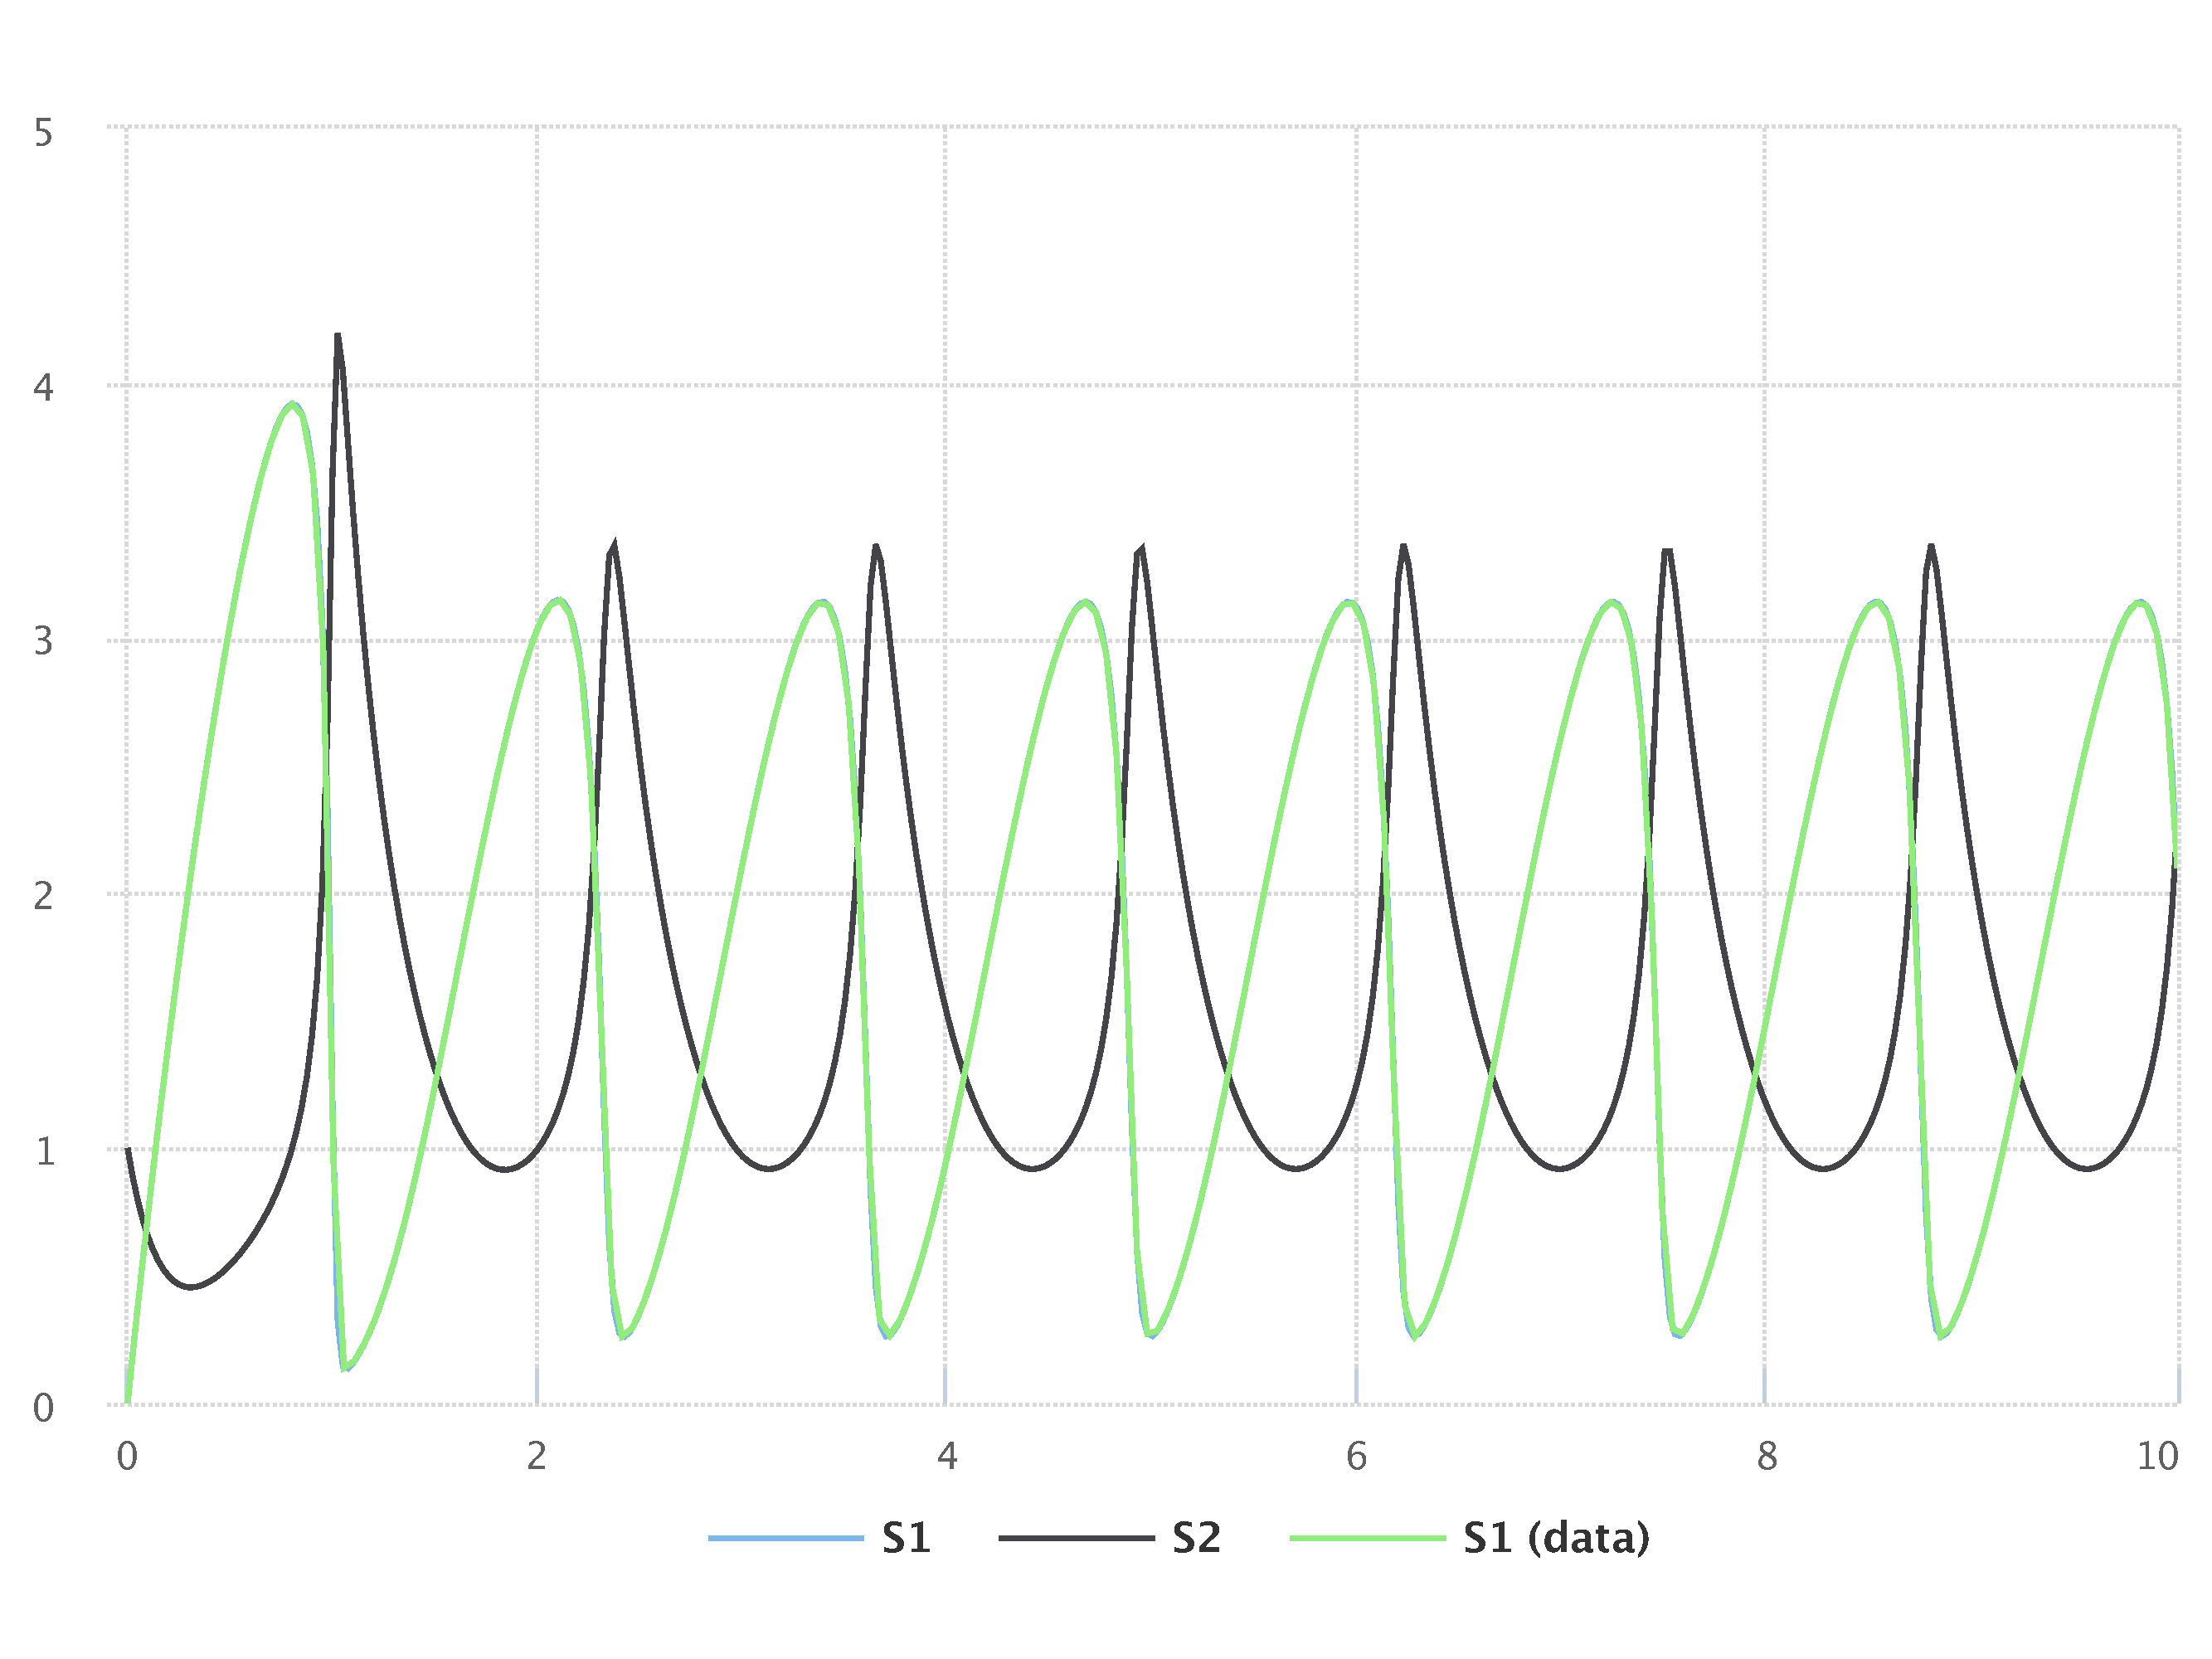
\includegraphics[width=1.0\textwidth]{examples/plotting-data-numl/results/sedml_webtools/plot1}
        \caption{The simulation result from the simulation description given in \lst{plotting-data-numl}. Simulation with SED-ML web tools \citep{bergmann2017sed}.}
    \end{minipage}\hfill
    \begin{minipage}{0.47\textwidth}
        \centering
        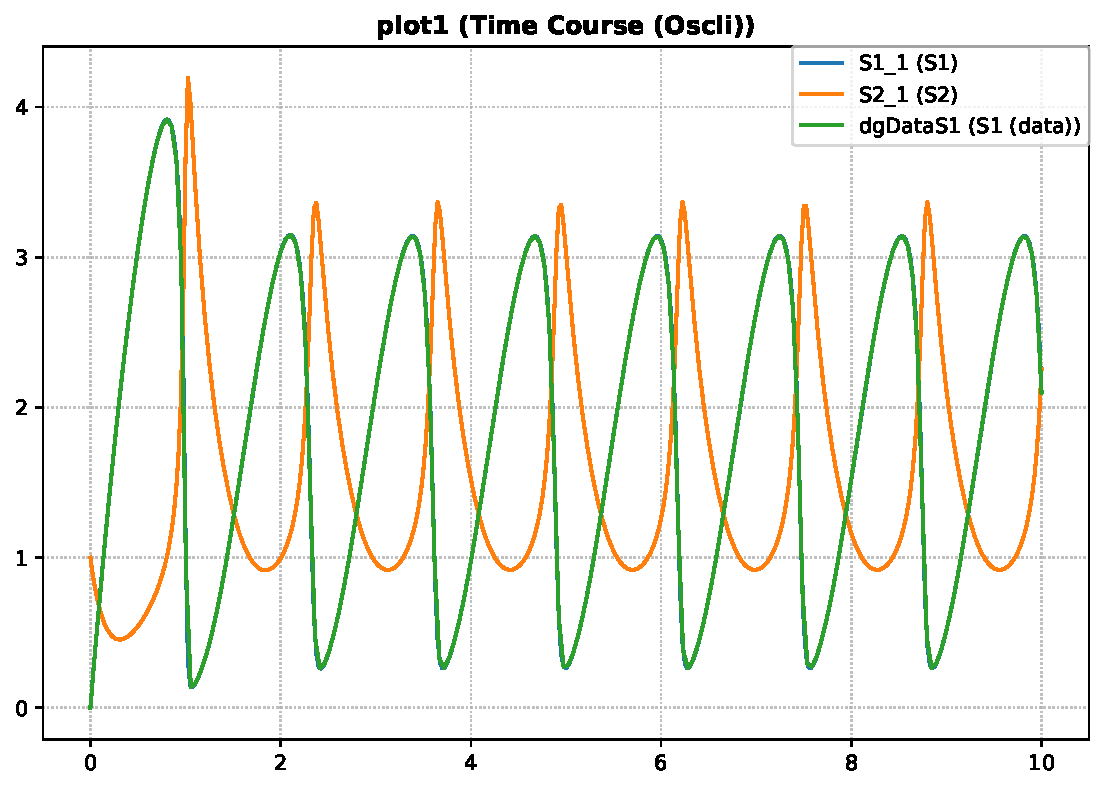
\includegraphics[width=1.0\textwidth]{examples/plotting-data-numl/results/tellurium/plot1}
        \caption{Simulation with tellurium \citep{tellurium}.}
    \end{minipage}
    \label{fig:plotting-data}
\end{figure}

\myXmlImport{SED-ML document using \SedDataSource and \SedDataDescription}
{lst:plotting-data-numl}
{examples/plotting-data-numl/plotting-data-numl.xml}

\pagebreak
% ~~~~~~~~~~~~~~~~~~~~~~~~~~~~~~~~~~~~
% REPEATED TASKS
% ~~~~~~~~~~~~~~~~~~~~~~~~~~~~~~~~~~~~
\section{Simulation experiments with repeatedTasks}
The \hyperref[class:repeatedTask]{RepeatedTask} makes it possible to encode a large number of different simulation experiments. In this section several such simulation experiments are presented.

% ~~~ TIME COURSE PARAMETER SCAN ~~~
\subsection{Time course parameter scan (\texttt{L1V3\_repeated-scan-oscli.omex})}
In this example a \hyperref[class:repeatedTask]{repeatedTask} is used to run repeated \hyperref[class:uniformTimeCourse]{uniformTimeCourse} simulations with a deterministic simulation algorithm. Within the \hyperref[class:repeatedTask]{repeatedTask} after each run the parameter value is changed, resulting in a time course parameter scan.

NOTE: This example produces three dimensional results (time, species concentration, multiple repeats).  SED-ML \currentLV does not include a way to post-process these values, so it is left to the implementation on how to display them. One example would be to flatten the values by overlaying them onto the desired plot.

\begin{figure}[ht]
    \centering
    \begin{minipage}{0.47\textwidth}
        \centering
        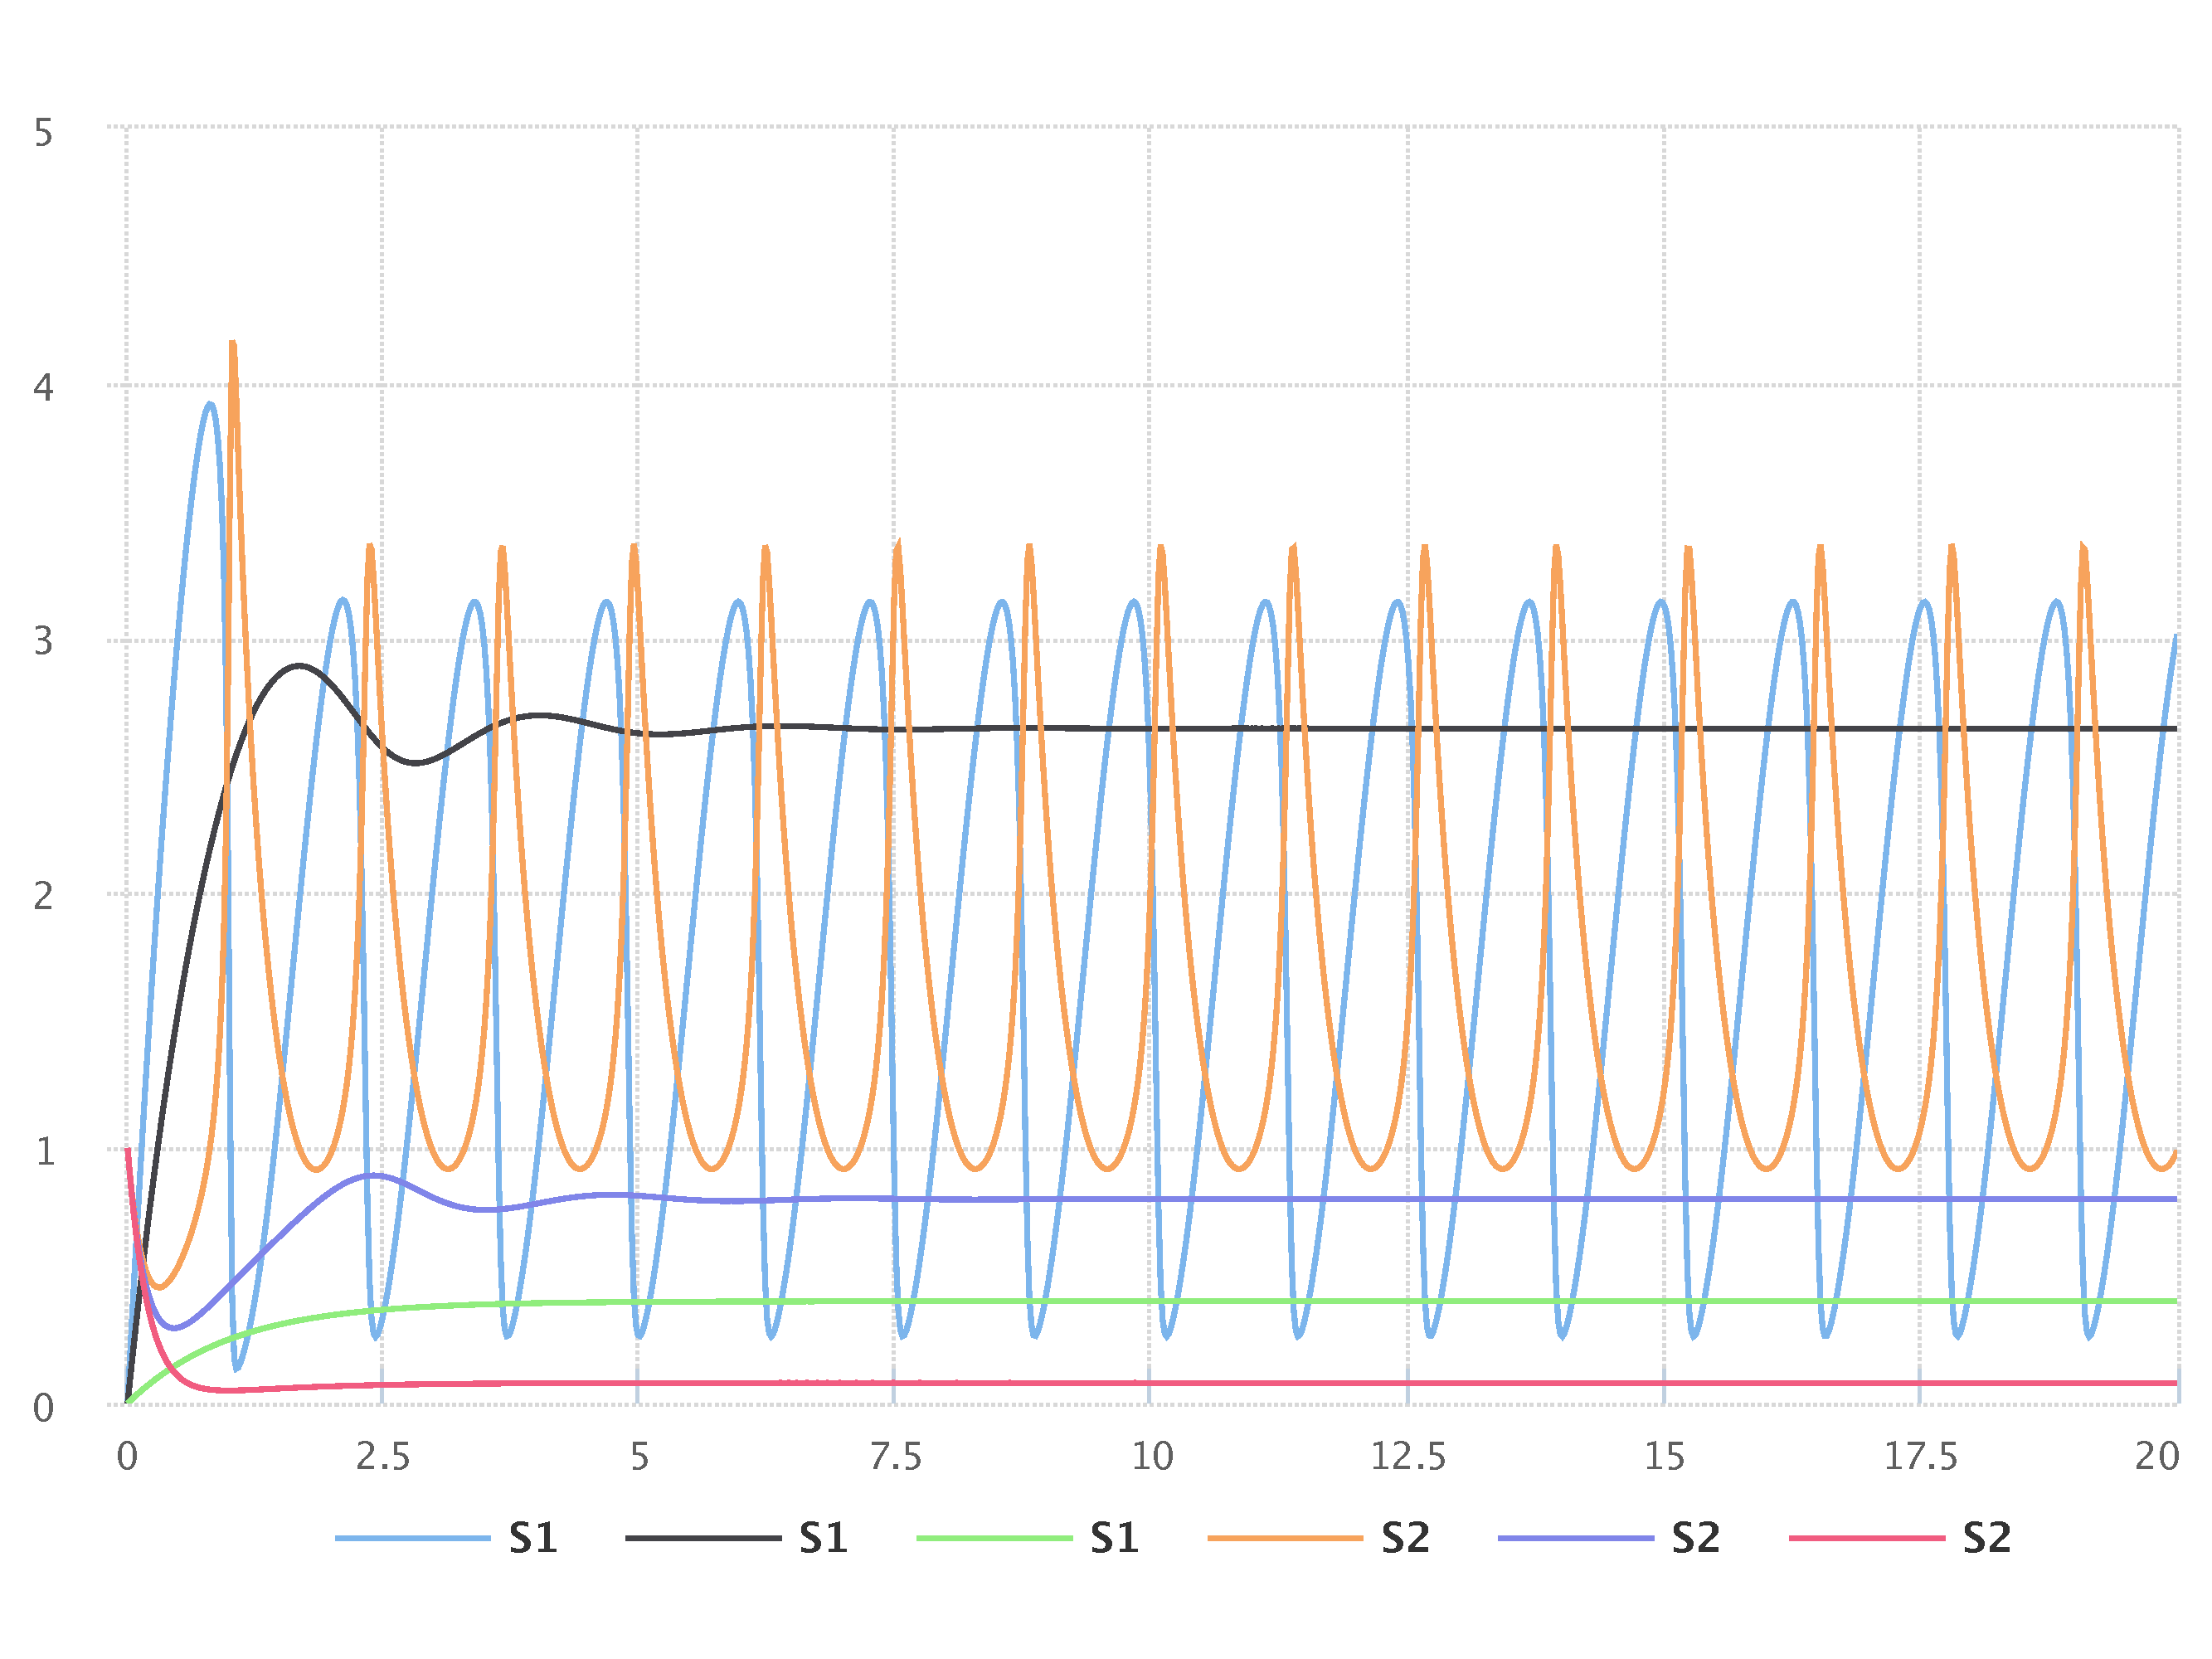
\includegraphics[width=1.0\textwidth]{examples/repeated-scan-oscli/results/sedml_webtools/plot1}
        \caption{The simulation result gained from the simulation description given in \lst{repeated-scan-oscli}. Simulation with SED-ML web tools \citep{bergmann2017sed}.}
    \end{minipage}\hfill
    \begin{minipage}{0.47\textwidth}
        \centering
                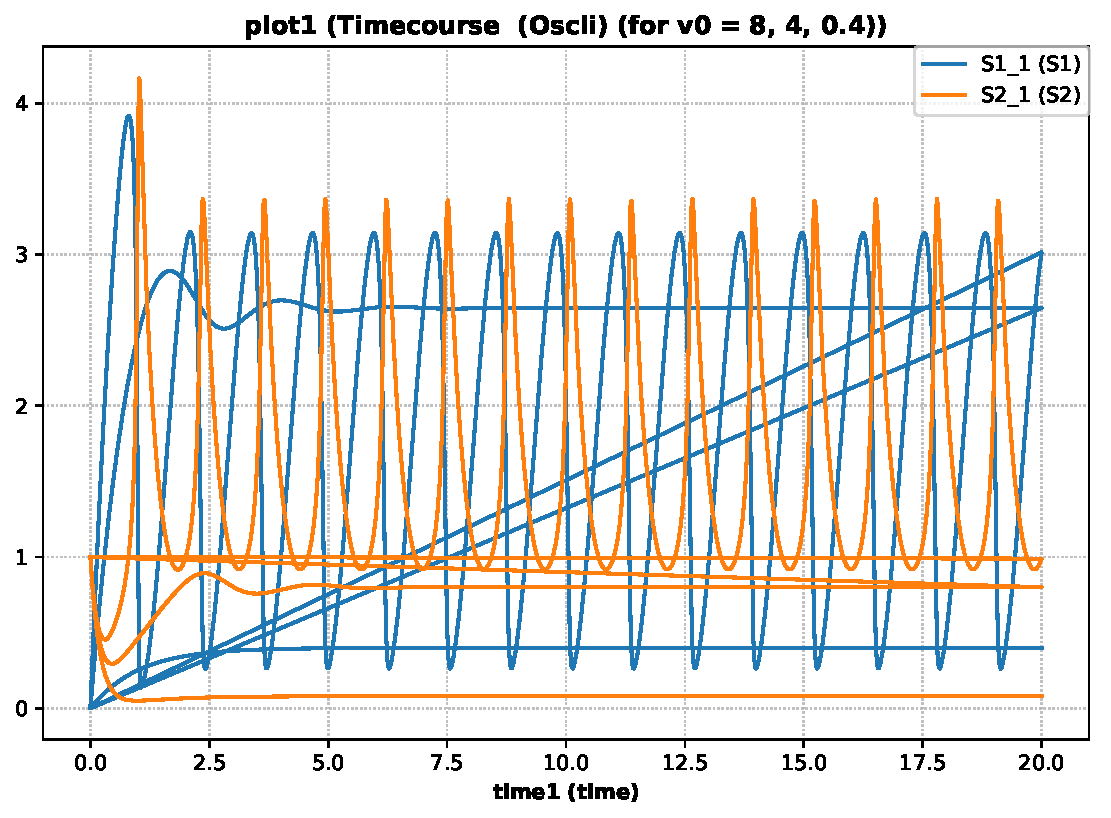
\includegraphics[width=1.0\textwidth]{examples/repeated-scan-oscli/results/tellurium/plot1}
        \caption{Simulation with tellurium \citep{tellurium}.}
    \end{minipage}
    \label{fig:repeated-scan-oscli}
\end{figure}

\myXmlImport{SED-ML document implementing the one dimensional time course parameter scan}
{lst:repeated-scan-oscli}
{examples/repeated-scan-oscli/repeated-scan-oscli.xml}

% ~~~ STEADY STATE PARAMETER SCAN ~~~
\subsection{Steady state parameter scan (\texttt{L1V3\_repeated-steady-scan-oscli.omex})}
In this example a \hyperref[class:repeatedTask]{repeatedTask} is used in combination with a \hyperref[class:steadyState]{steadyState} simulation task (performing a steady state computation). On each repeat a parameter is varied resulting in a steady state parameter scan.

\begin{figure}[ht!]
    \centering
    \begin{minipage}{0.47\textwidth}
        \centering
        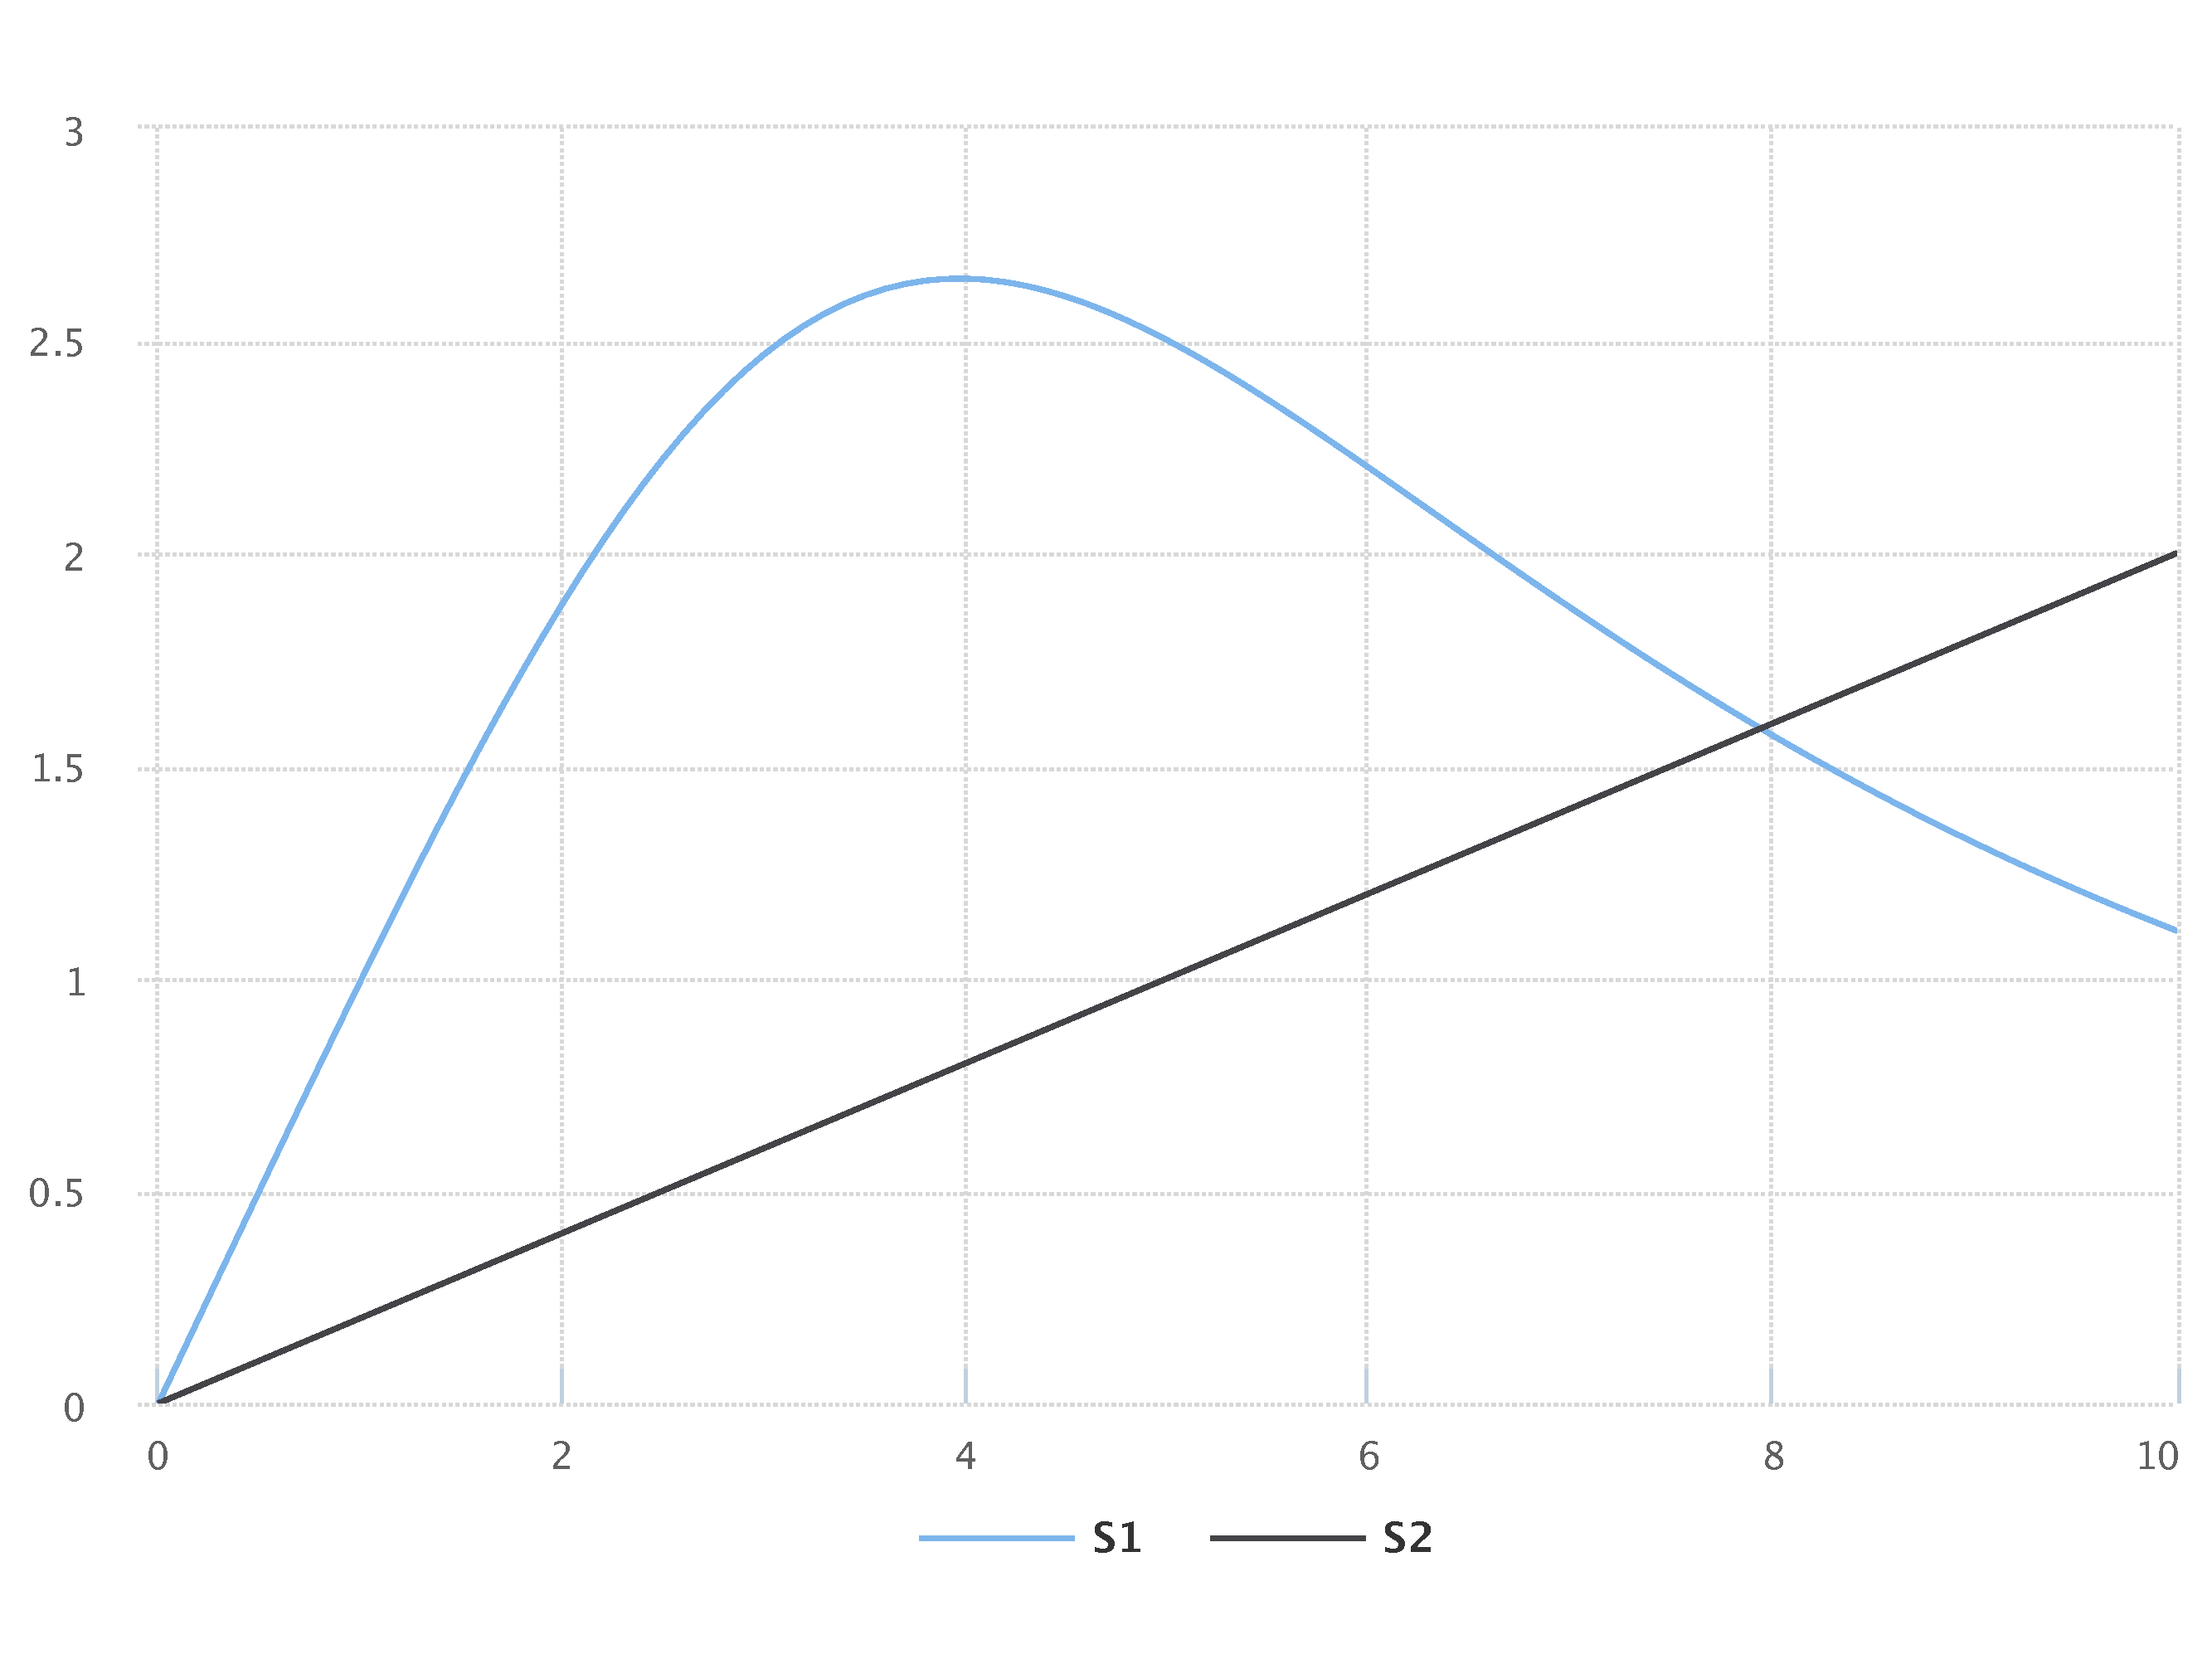
\includegraphics[width=1.0\textwidth]{examples/repeated-steady-scan-oscli/results/sedml_webtools/plot1}
        \caption{The simulation result from the simulation description given in \lst{repeated-steady-scan-oscli}. Simulation with SED-ML web tools \citep{bergmann2017sed}.}
    \end{minipage}\hfill
    \begin{minipage}{0.47\textwidth}
        \centering
        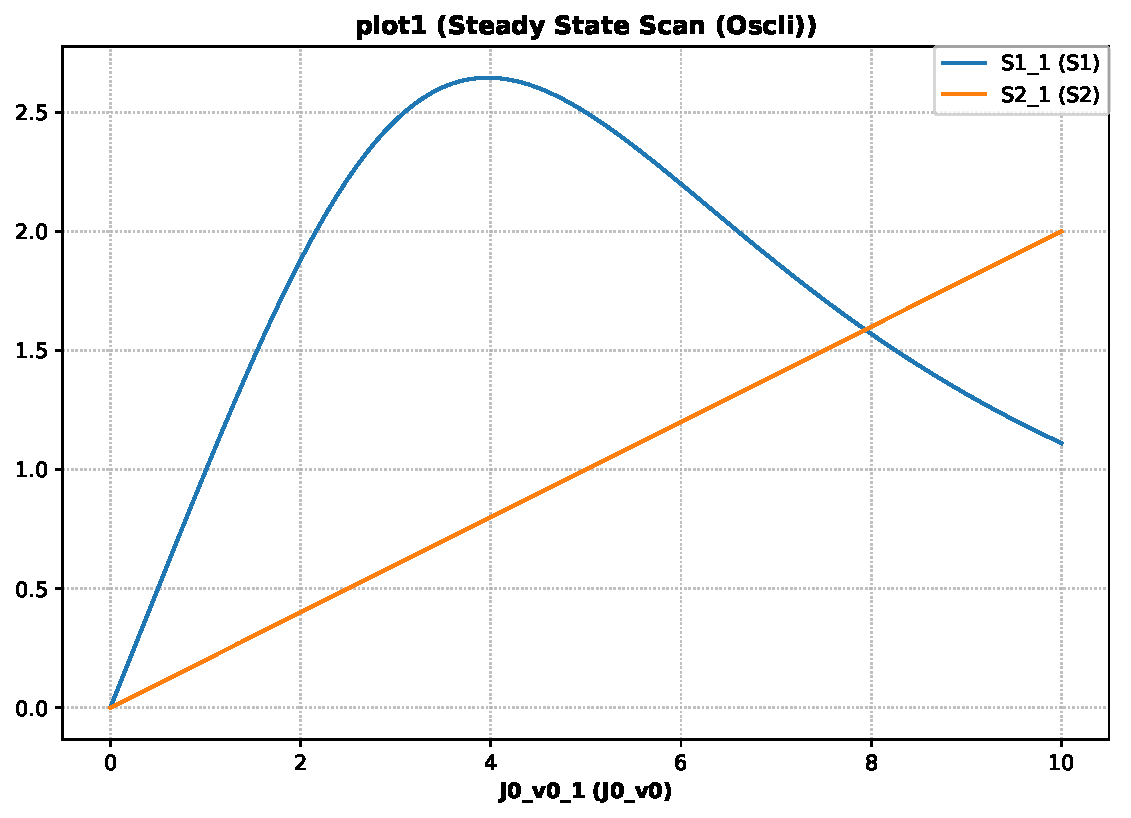
\includegraphics[width=1.0\textwidth]{examples/repeated-steady-scan-oscli/results/tellurium/plot1}
        \caption{Simulation with tellurium \citep{tellurium}.}
    \end{minipage}
    \label{fig:repeated-steady-scan-oscli}
\end{figure}

\myXmlImport{SED-ML document implementing the one dimensional steady state parameter scan}
{lst:repeated-steady-scan-oscli}
{examples/repeated-steady-scan-oscli/repeated-steady-scan-oscli.xml}


% ~~~ STOCHASTIC SIMULATION ~~~
\subsection{Stochastic simulation (\texttt{L1V3\_repeated-stochastic-runs.omex})}
In this example a \hyperref[class:repeatedTask]{repeatedTask} is used to run a stochastic simulation multiple times.
Running just one stochastic trace does not provide a complete picture of the behavior of a system. A large number of such traces is needed. This example demonstrates the basic use case of running ten traces of a simulation by using a \hyperref[class:repeatedTask]{repeatedTask} which runs ten uniform time course simulations (each performing a stochastic simulation run).

NOTE: This example produces three dimensional results (time, species concentration, multiple repeats). While SED-ML \currentLV does not include a way to post-processing these values. So it is left to the implementation on how to display them. One example would be to flatten the values by overlaying them onto the desired plot. 

\begin{figure}[ht]
    \centering
    \begin{minipage}{0.47\textwidth}
        \centering
        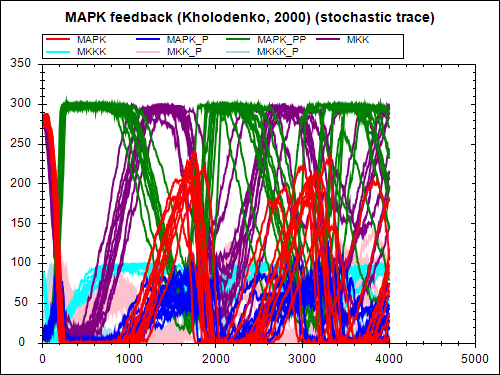
\includegraphics[width=1.0\textwidth]{examples/repeated-stochastic-runs/results/sedml_webtools/plot1}
        \caption{The simulation result from the simulation description given in \lst{repeated-stochastic-runs}. Simulation with SED-ML web tools \citep{bergmann2017sed}.}
    \end{minipage}\hfill
    \begin{minipage}{0.47\textwidth}
        \centering
        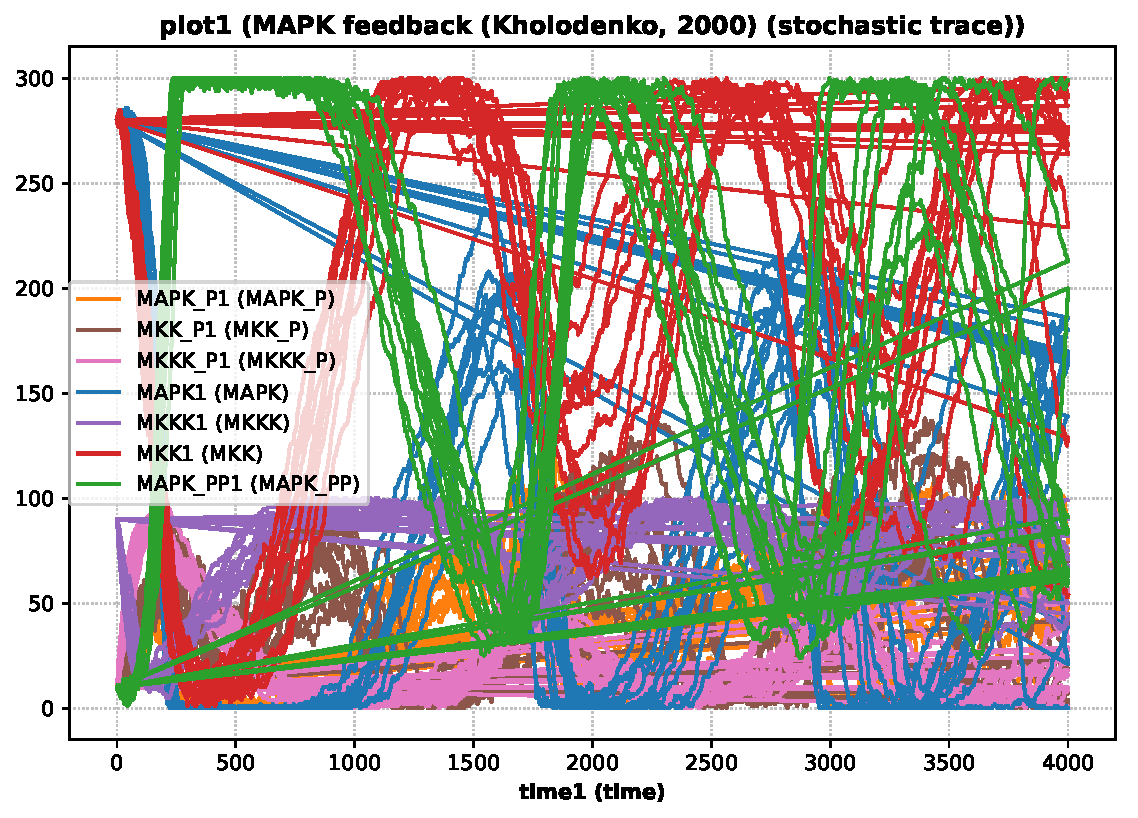
\includegraphics[width=1.0\textwidth]{examples/repeated-stochastic-runs/results/tellurium/plot1}
        \caption{Simulation with tellurium \citep{tellurium}.}
    \end{minipage}
    \label{fig:repeated-stochastic-runs}
\end{figure}

\myXmlImport{SED-ML document implementing repeated stochastic runs}
{lst:repeated-stochastic-runs}
{examples/repeated-stochastic-runs/repeated-stochastic-runs.xml}


% ~~~ SIMULATION PERTURBATION ~~~
\subsection{Simulation perturbation (\texttt{L1V3\_oscli-nested-pulse.omex})}
Often it is interesting to see how the dynamic behavior of a model changes when some perturbations are applied to the model. In this example a \hyperref[class:repeatedTask]{repeatedTask} is used iterating a \hyperref[class:oneStep]{oneStep} task (that advances an ODE integration to the next output step). During the steps a single parameter is modified effectively causing the oscillations of a model to stop. Once the value is reset the oscillations recover. 

Note: In the example a \hyperref[class:functionalRange]{functionalRange} is used, although the same result could also be achieved using the \hyperref[class:setValue]{setValue} element directly.

\begin{figure}[ht]
    \centering
    \begin{minipage}{0.47\textwidth}
        \centering
        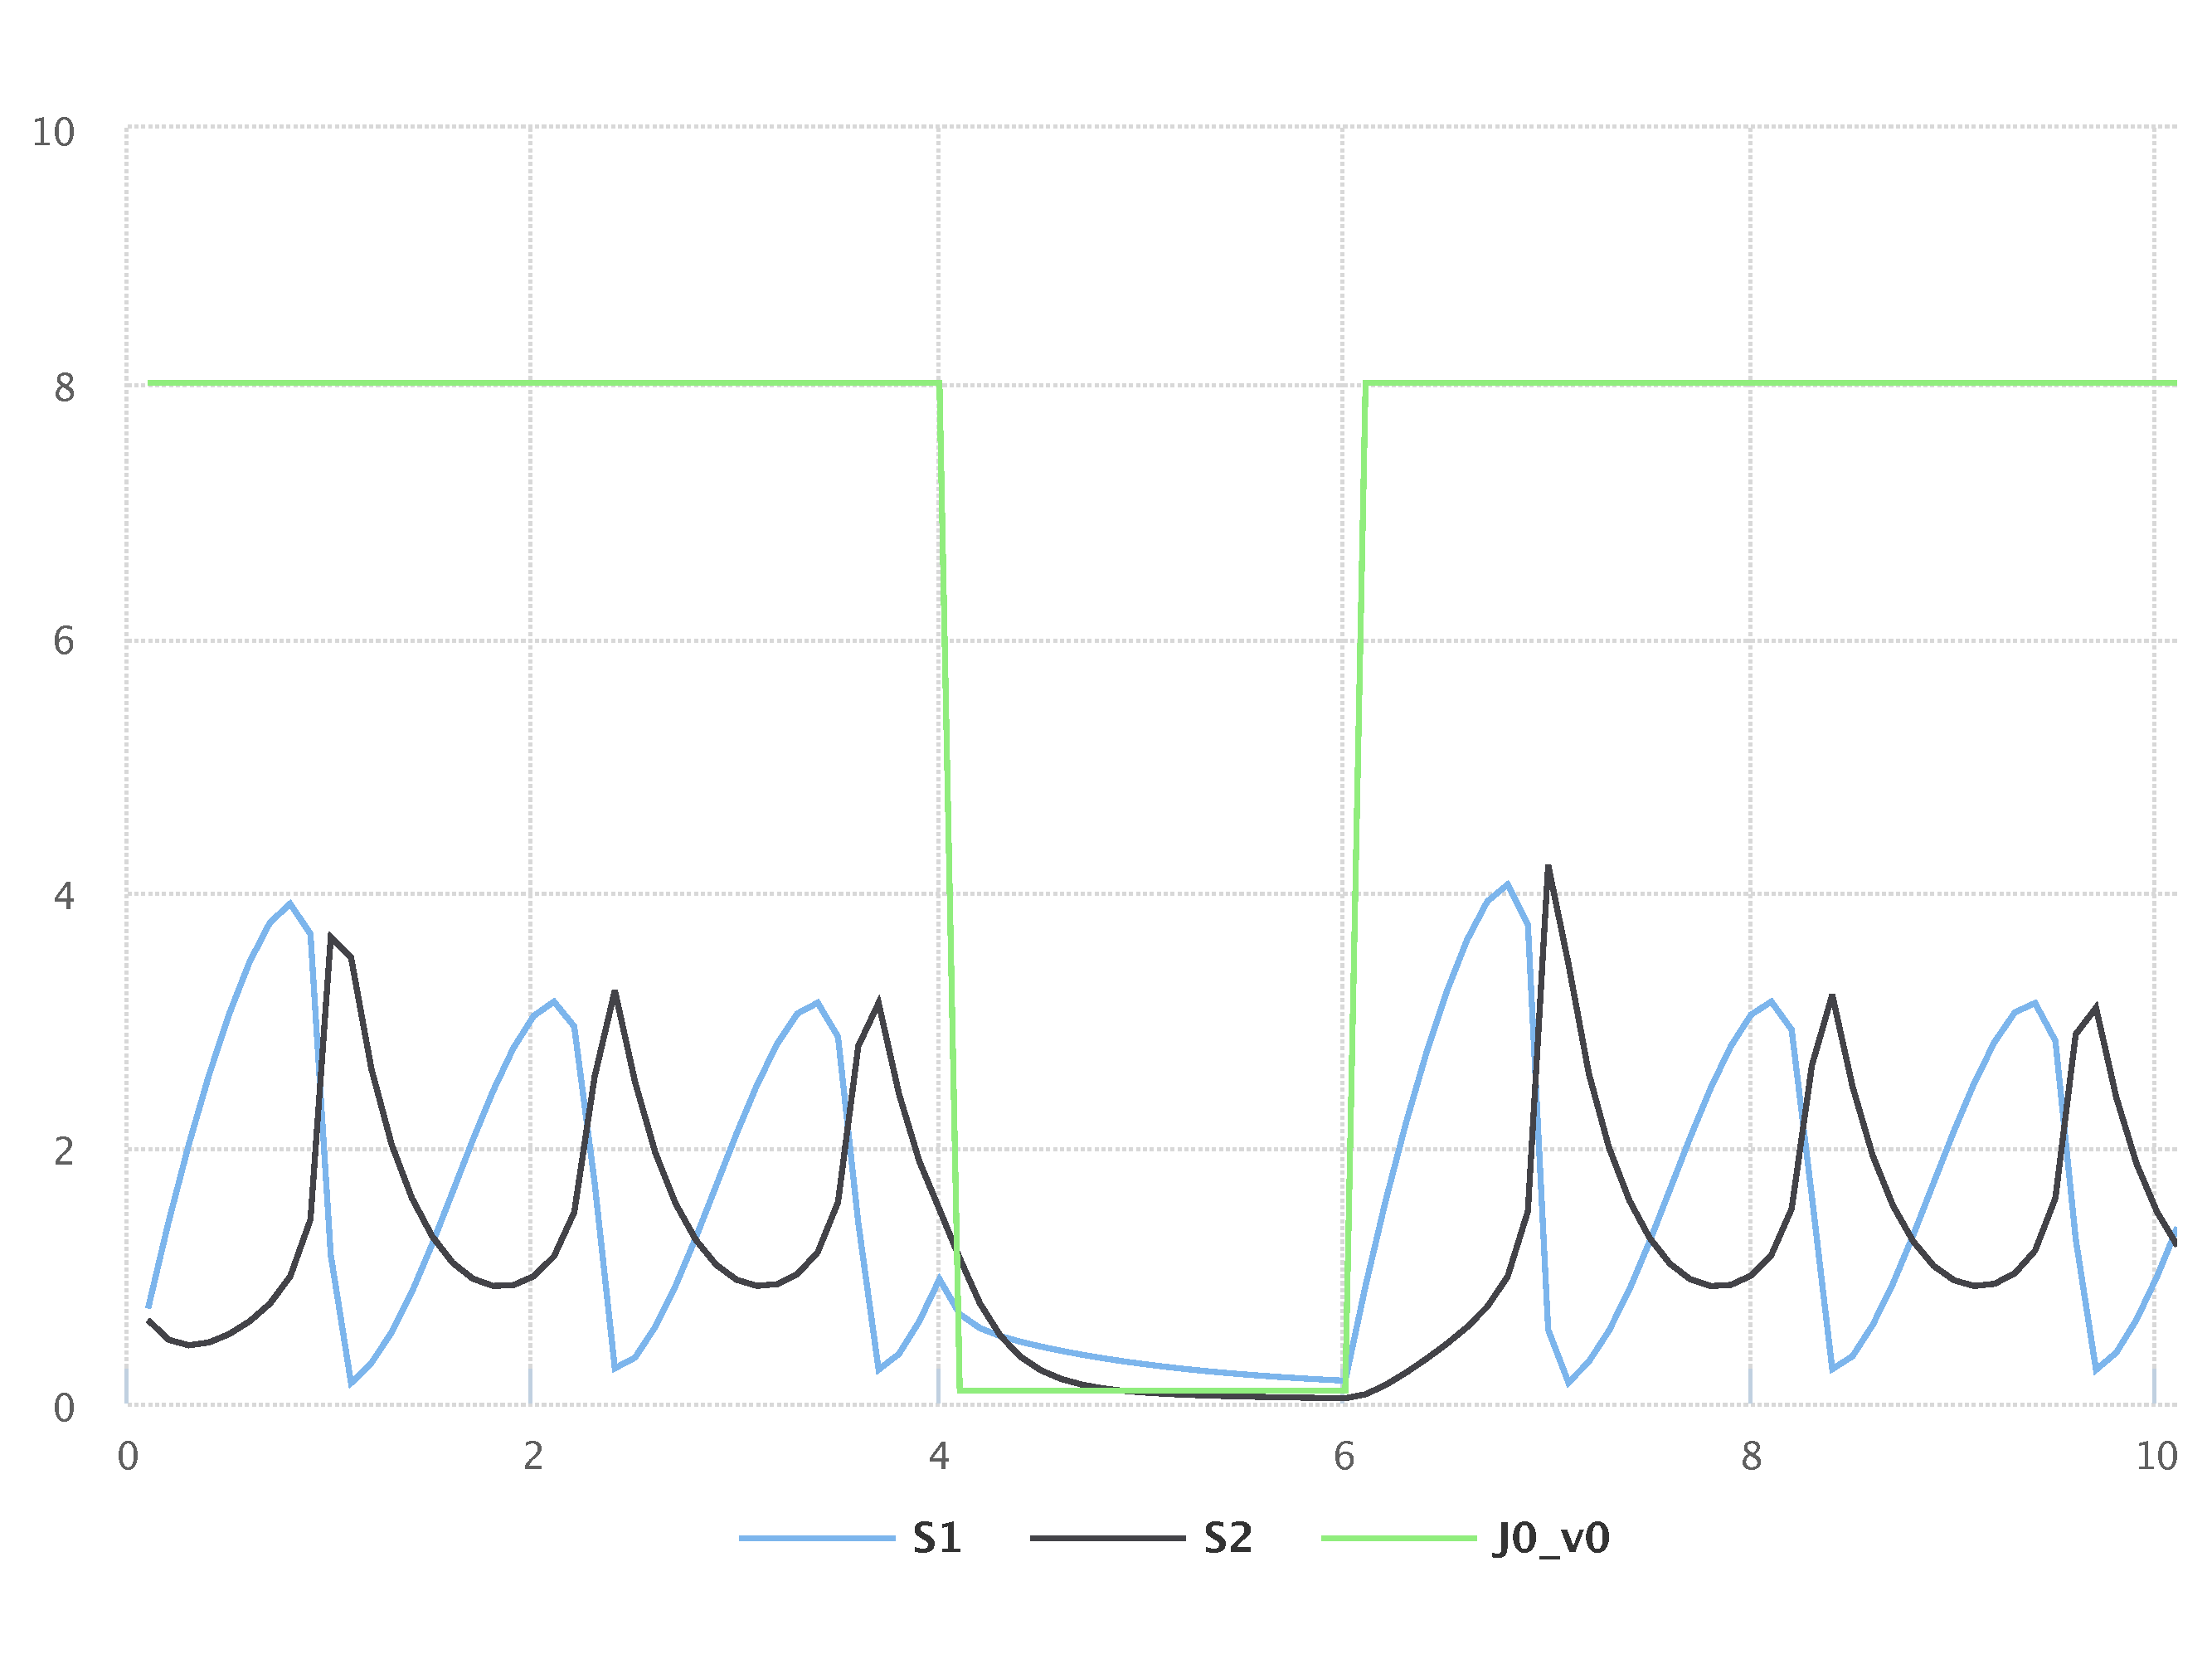
\includegraphics[width=1.0\textwidth]{examples/oscli-nested-pulse/results/sedml_webtools/plot1}
        \caption{The simulation result from the simulation description given in \lst{oscli-nested-pulse}. Simulation with SED-ML web tools \citep{bergmann2017sed}.}
    \end{minipage}\hfill
    \begin{minipage}{0.47\textwidth}
        \centering
        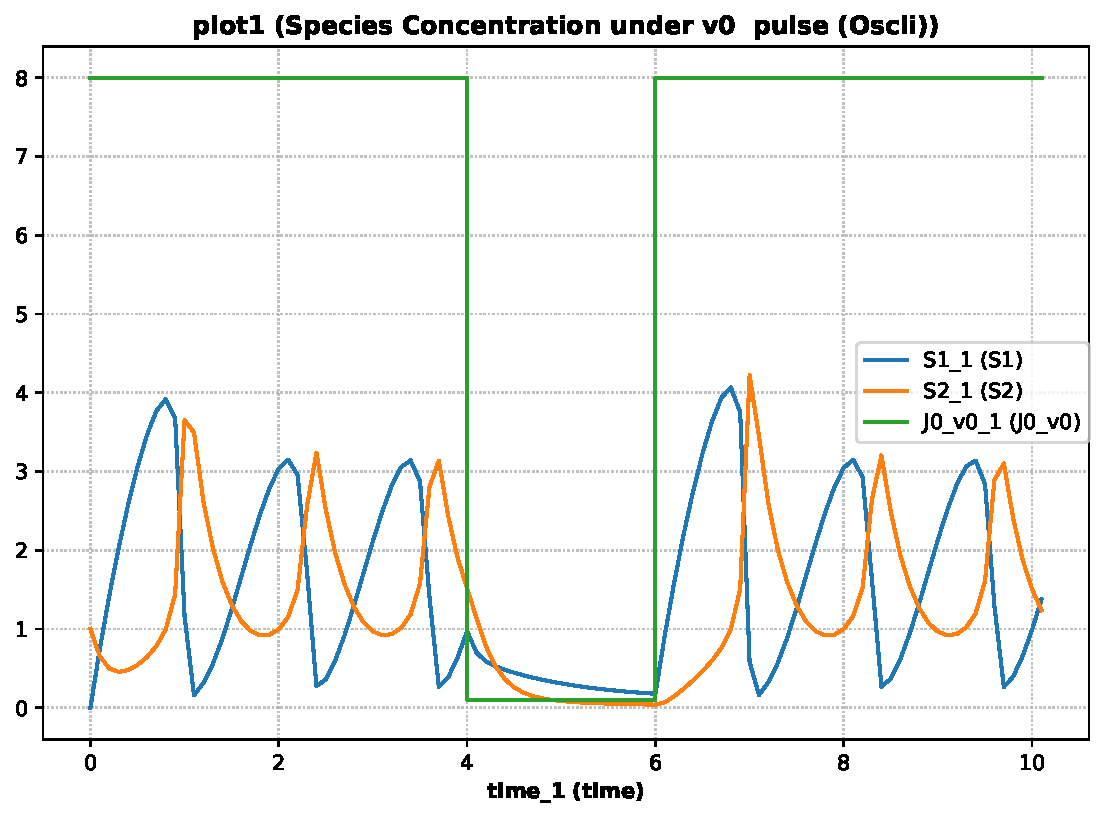
\includegraphics[width=1.0\textwidth]{examples/oscli-nested-pulse/results/tellurium/plot1}
        \caption{Simulation with tellurium \citep{tellurium}.}
    \end{minipage}
    \label{fig:oscli-nested-pulse}
\end{figure}

\myXmlImport{SED-ML document implementing the perturbation experiment}
{lst:oscli-nested-pulse}
{examples/oscli-nested-pulse/oscli-nested-pulse.xml}


% ~~~ 2D STEADY STATE PARAMETER SCAN ~~~
\subsection{2D steady state parameter scan (\texttt{L1V3\_parameter-scan-2d.omex})}
This example uses a \hyperref[class:repeatedTask]{repeatedTask} which runs over another \hyperref[class:repeatedTask]{repeatedTask} which performs a steady state computation. Each repeated simulation task modifies a different parameter.

NOTE: This example produces three dimensional results (time, species concentration, multiple repeats). While SED-ML \currentLV does not include a way to post-processing these values. So it is left to the implementation on how to display them. One example would be to flatten the values by overlaying them onto the desired plot. 

\begin{figure}[ht]
    \centering
    \begin{minipage}{0.47\textwidth}
        \centering
        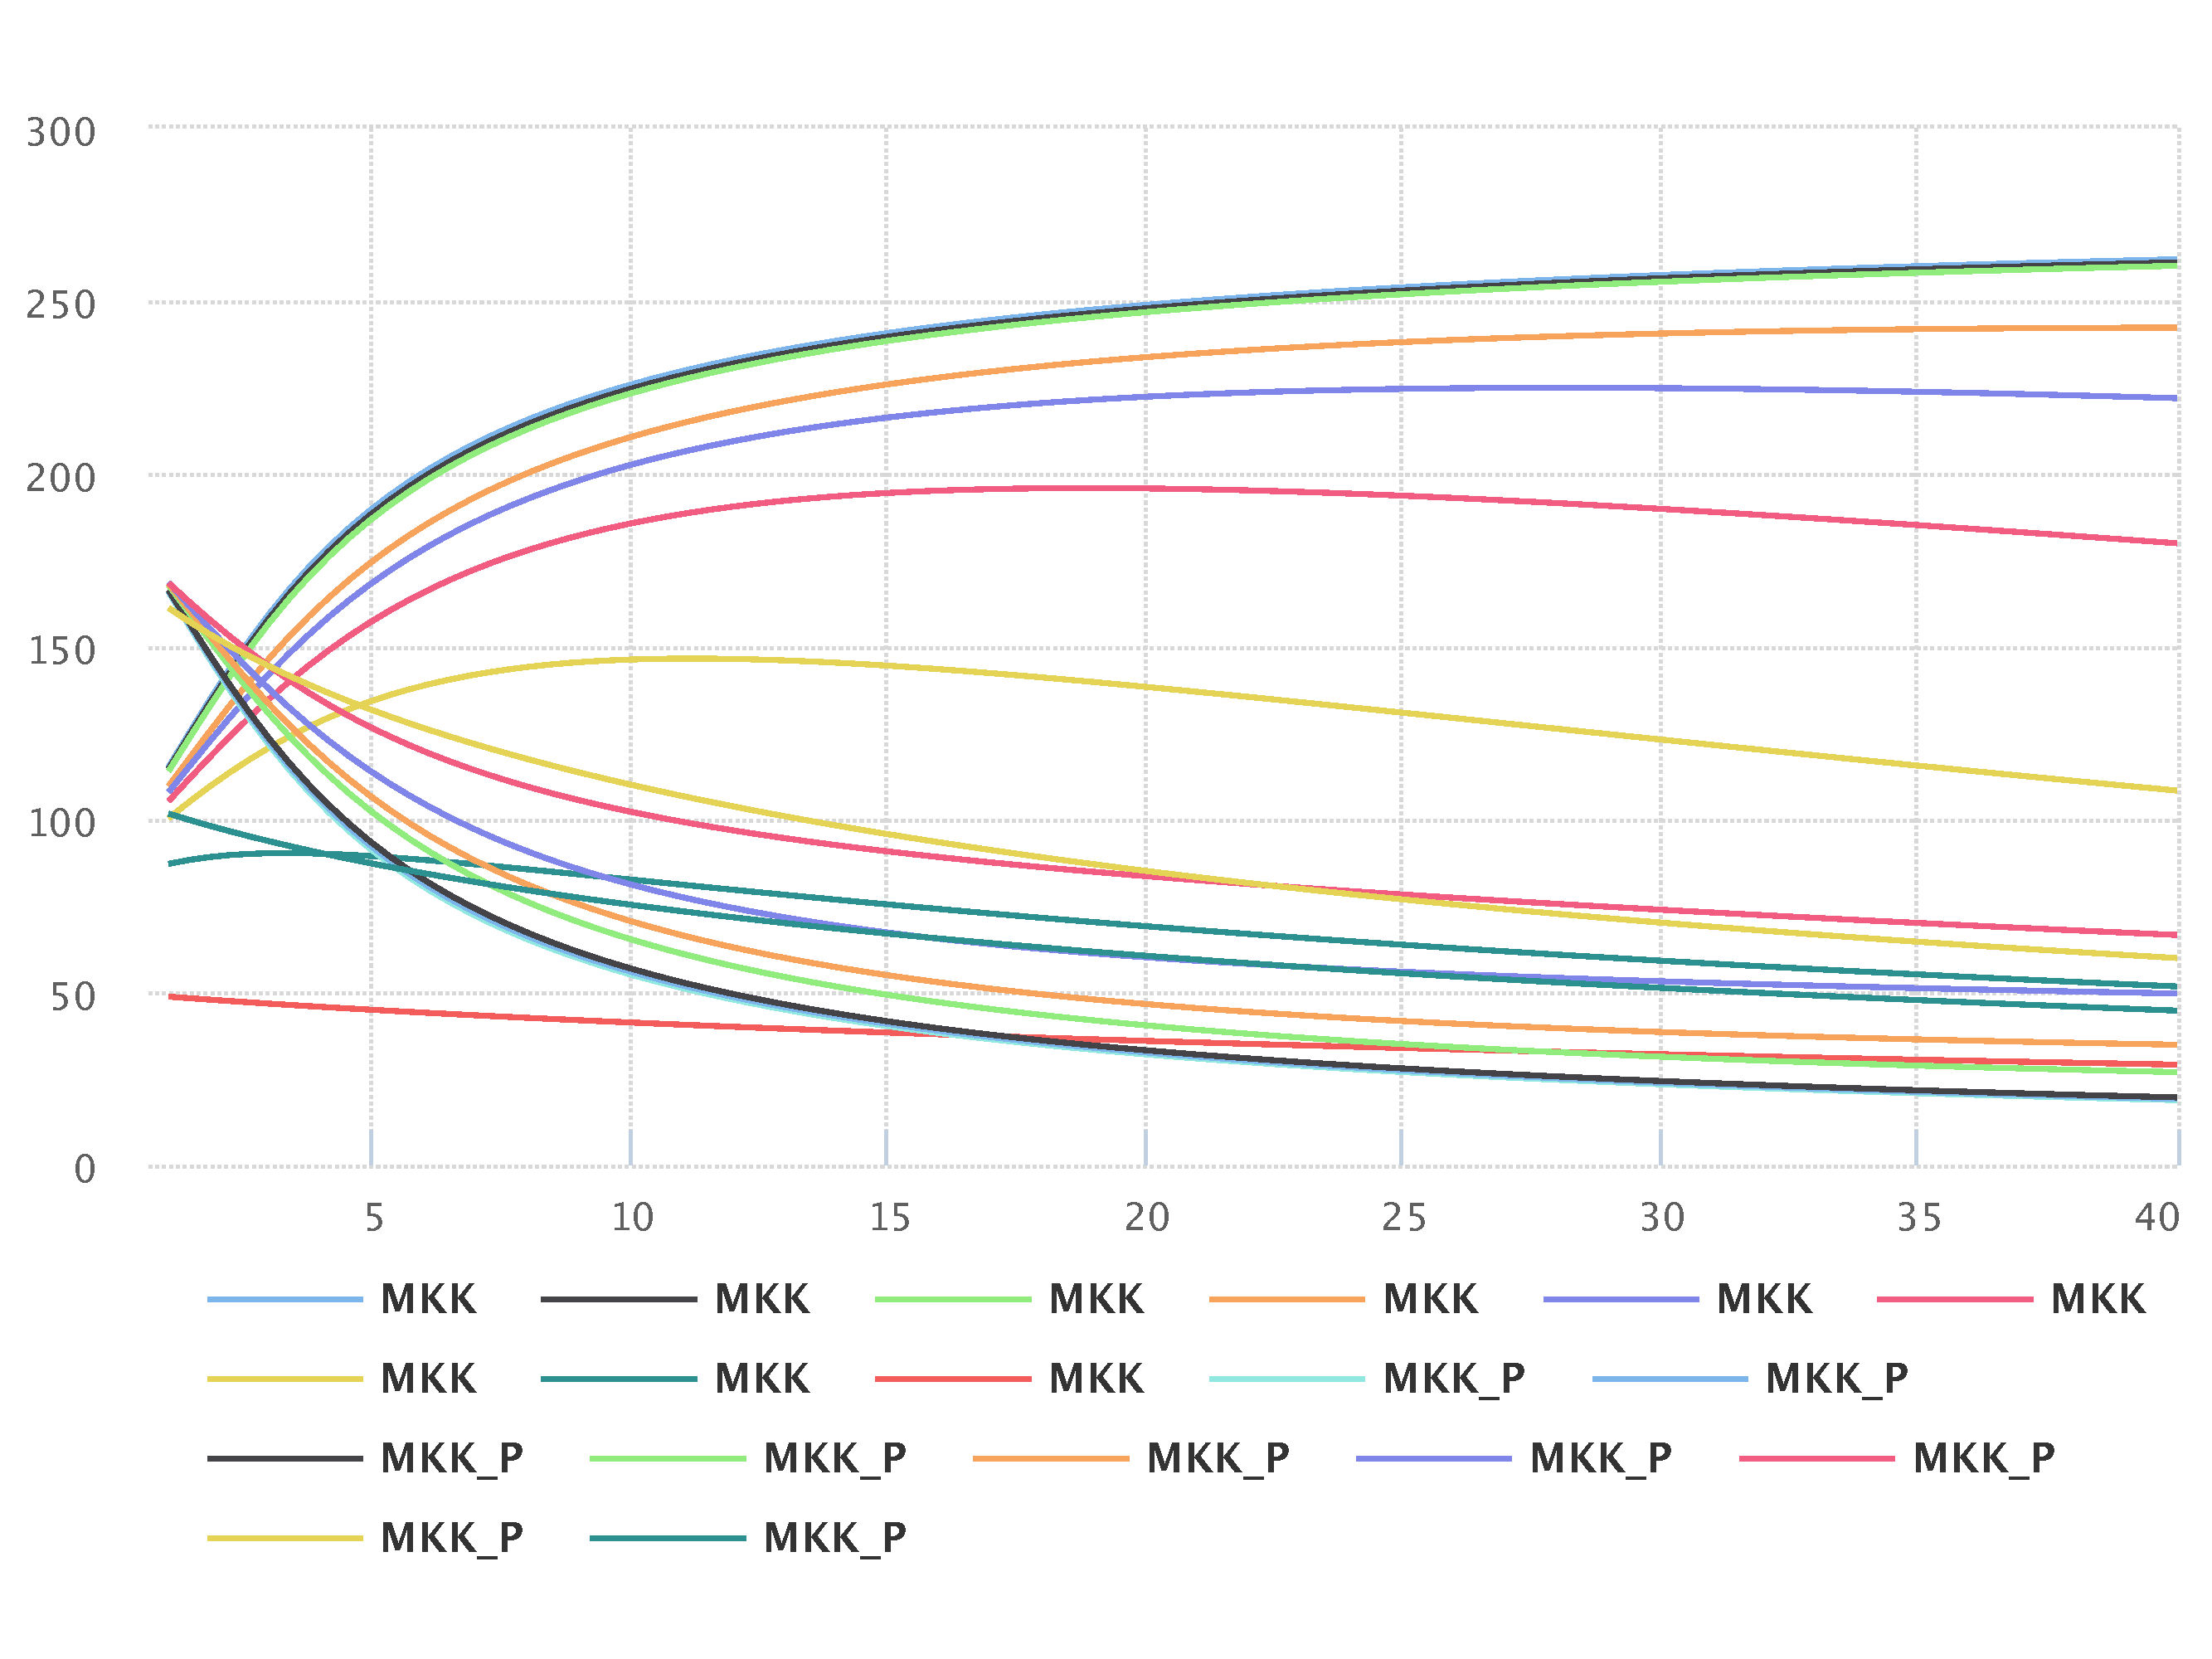
\includegraphics[width=1.0\textwidth]{examples/parameter-scan-2d/results/sedml_webtools/plot1}
        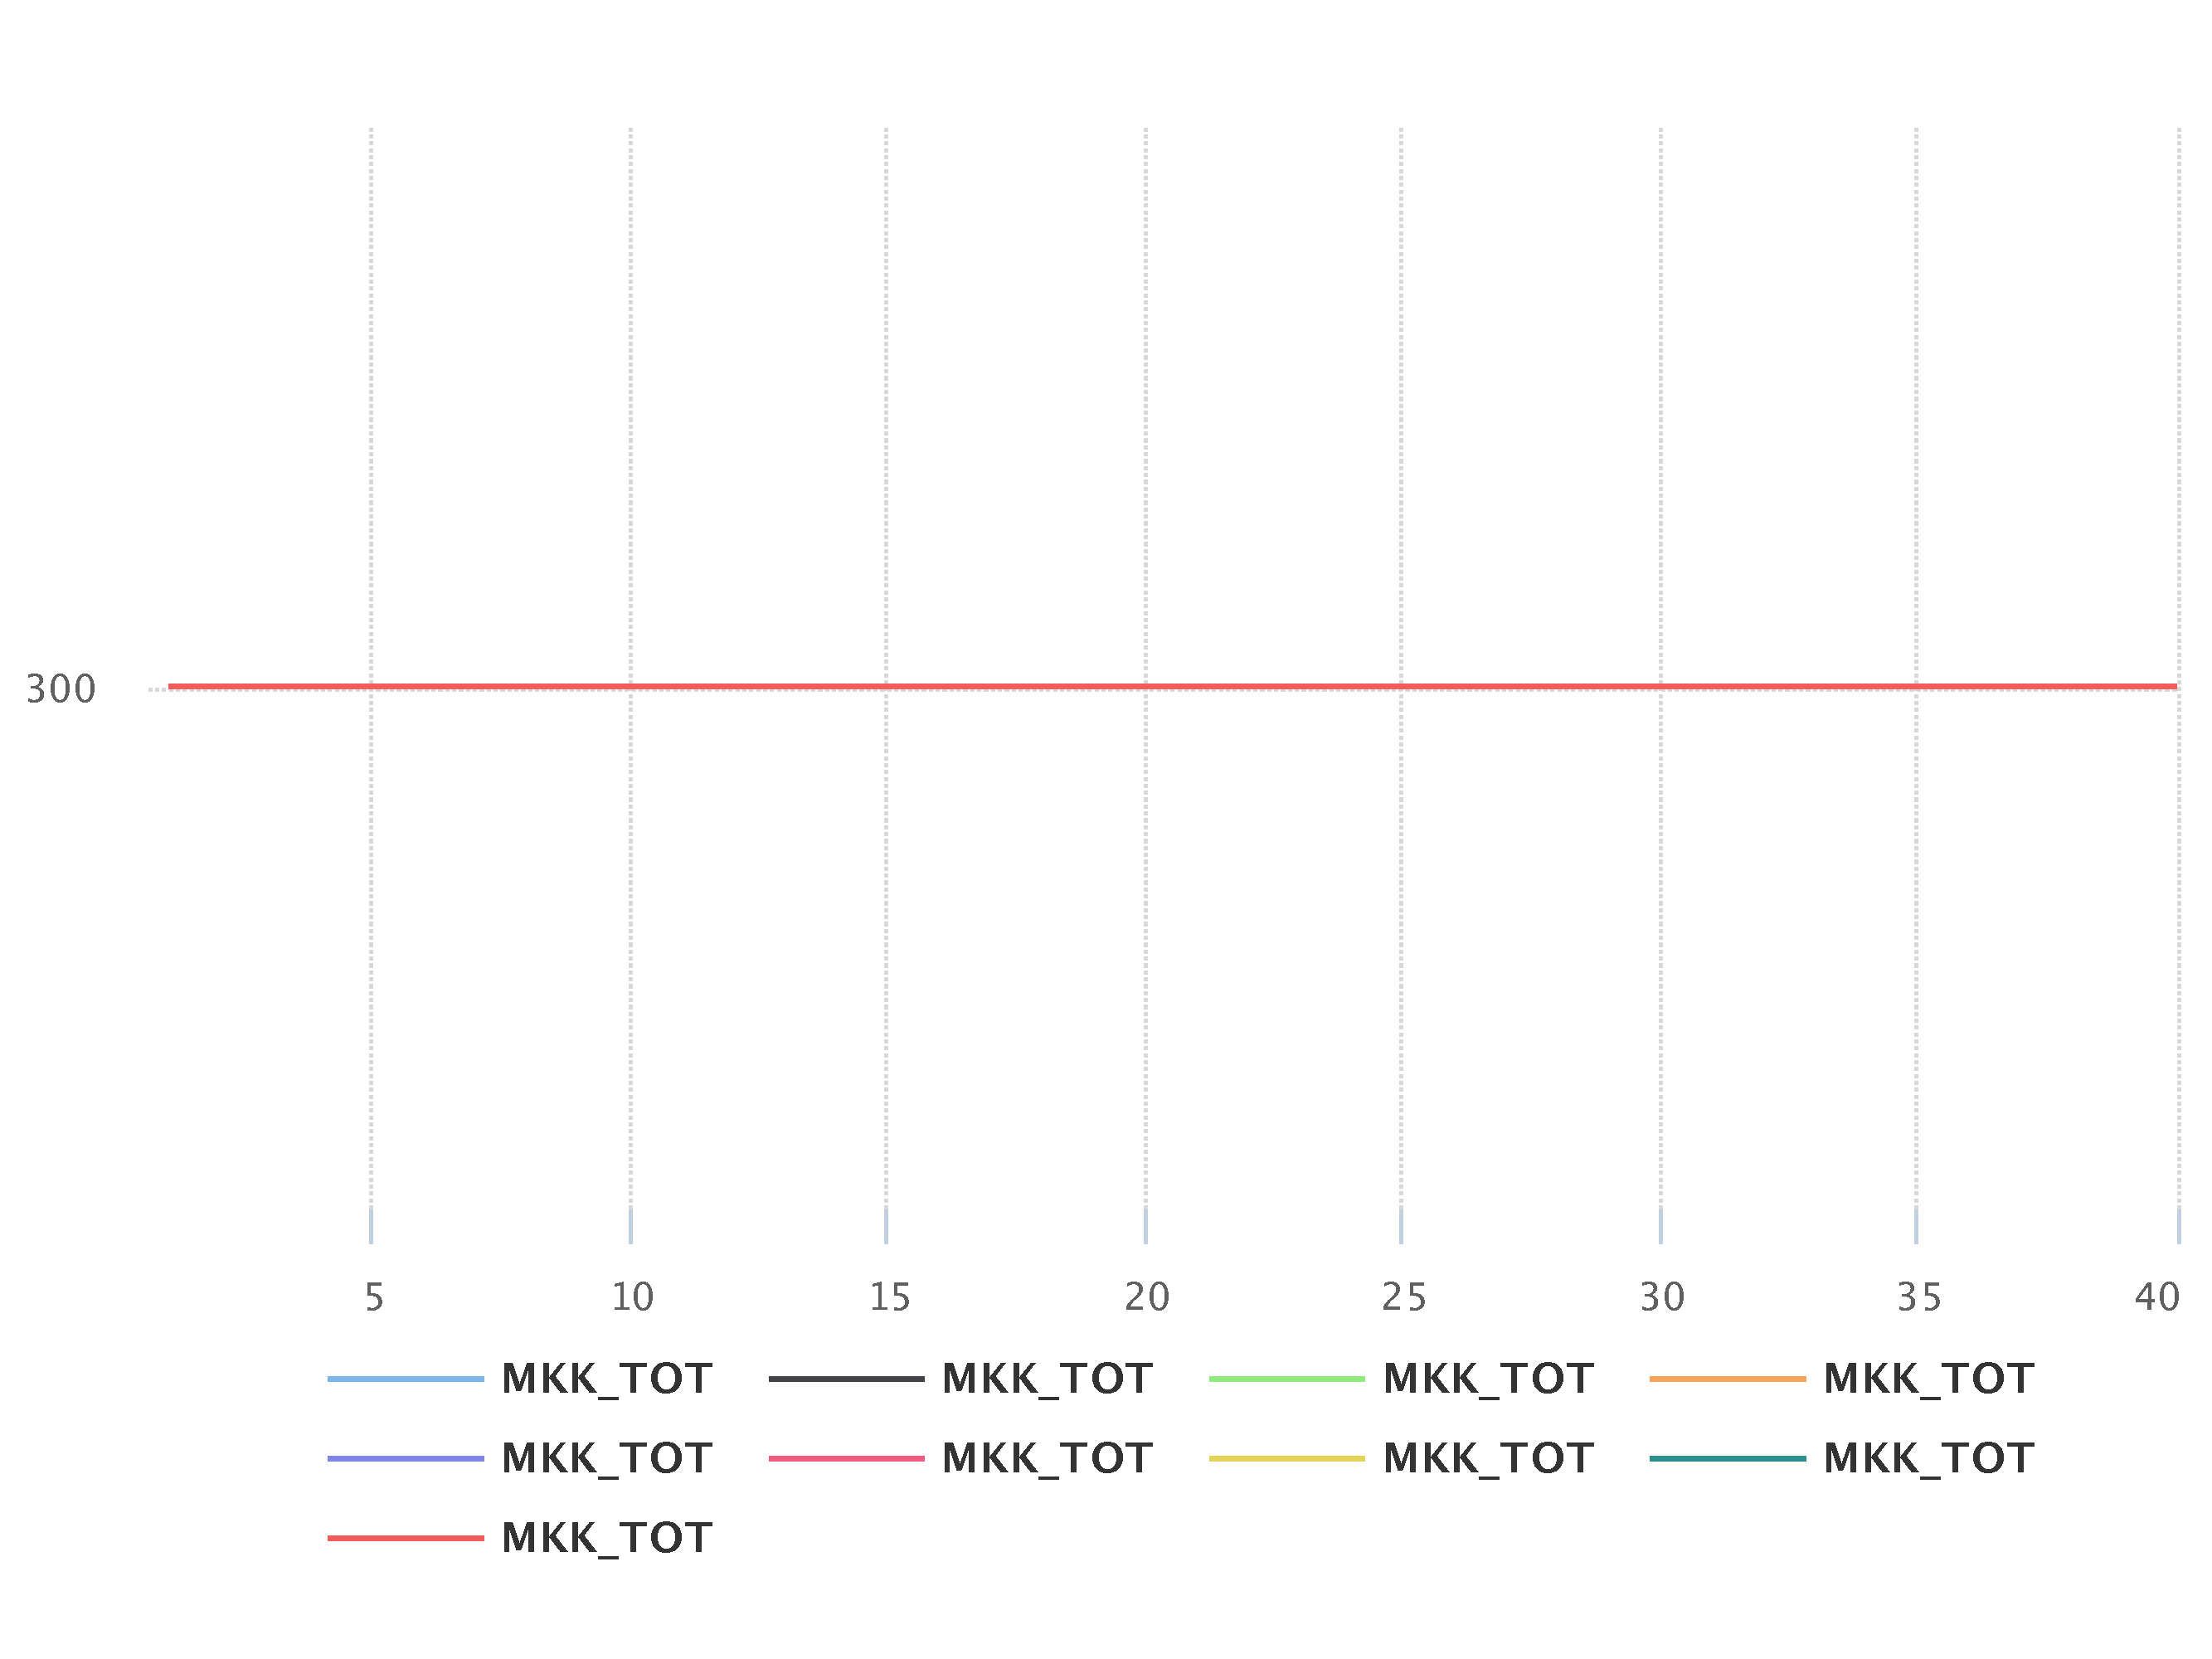
\includegraphics[width=1.0\textwidth]{examples/parameter-scan-2d/results/sedml_webtools/plot2}
        \caption{The simulation result gained from the simulation description given in \lst{parameter-scan-2d}. Simulation with SED-ML web tools \citep{bergmann2017sed}.}
    \end{minipage}\hfill
    \begin{minipage}{0.47\textwidth}
        \centering
        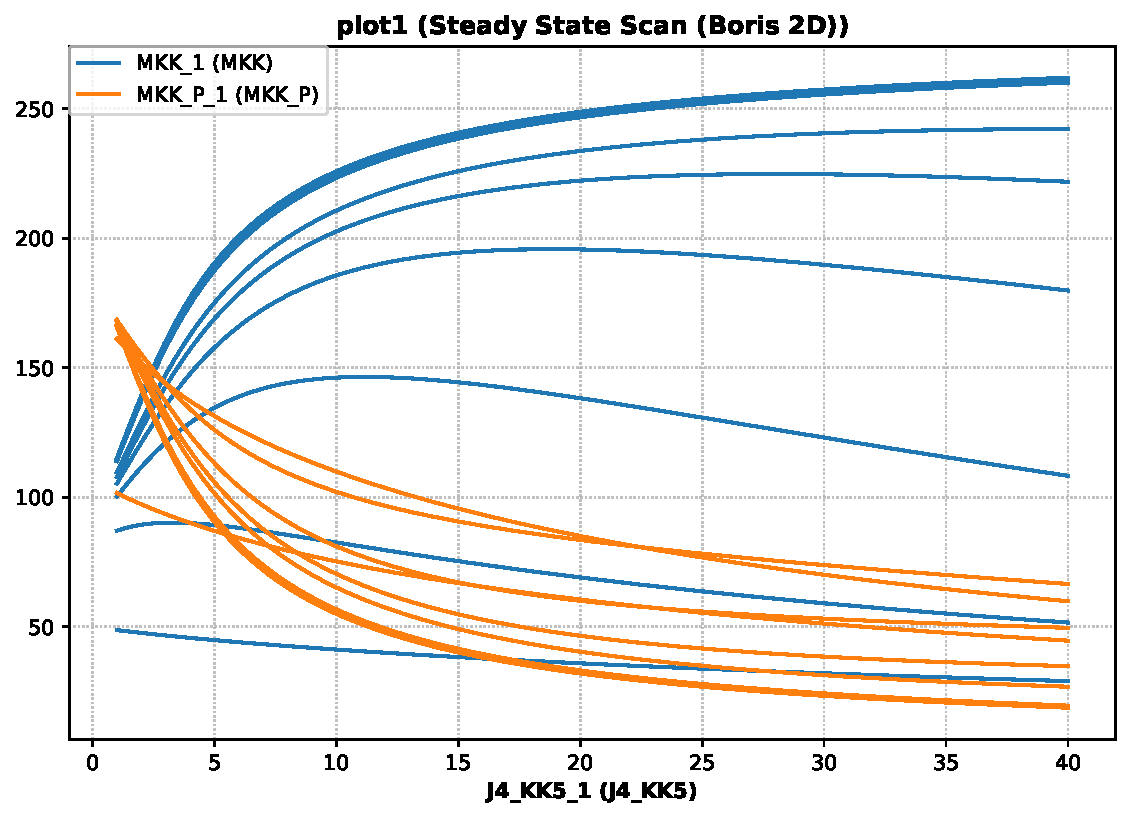
\includegraphics[width=1.0\textwidth]{examples/parameter-scan-2d/results/tellurium/plot1}
		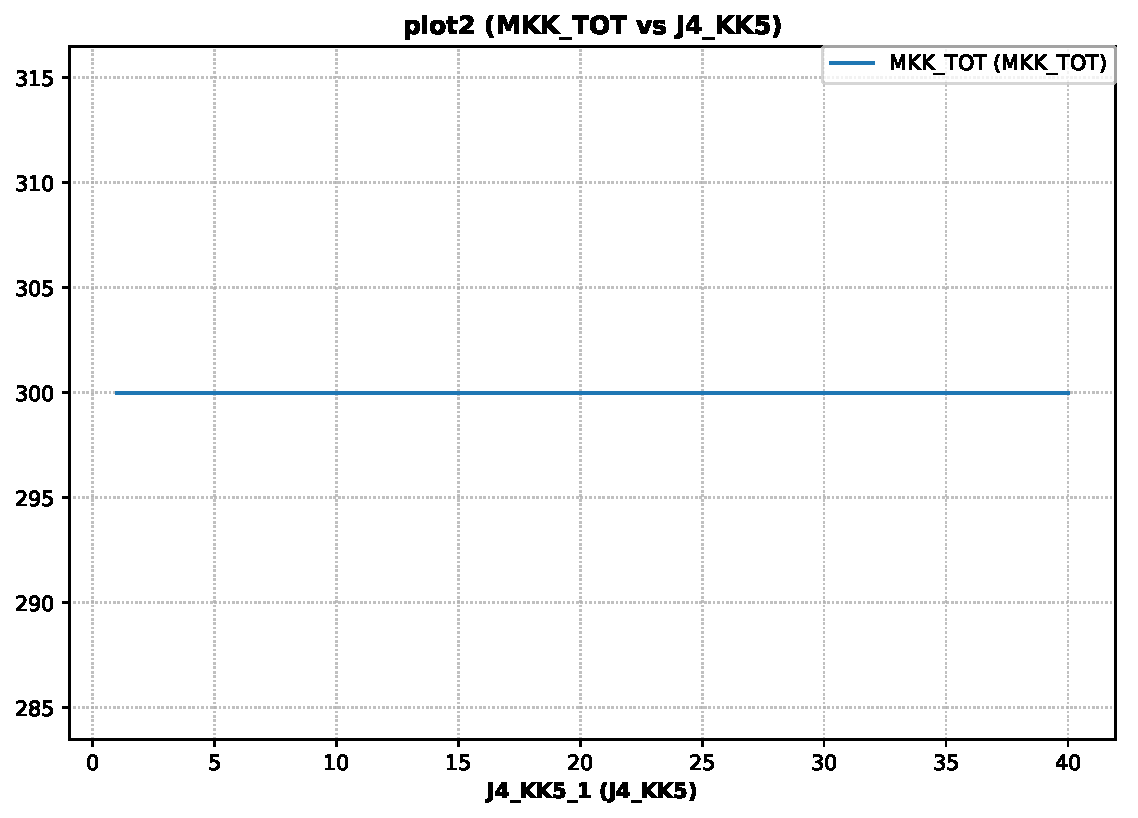
\includegraphics[width=1.0\textwidth]{examples/parameter-scan-2d/results/tellurium/plot2}
        \caption{Simulation with tellurium \citep{tellurium}.}
    \end{minipage}
    \label{fig:parameter-scan-2d}
\end{figure}

\myXmlImport{SED-ML document implementing the two dimensional steady state parameter scan}
{lst:parameter-scan-2d}
{examples/parameter-scan-2d/parameter-scan-2d.xml}

\pagebreak
% ~~~~~~~~~~~~~~~~~~~~~~~~~~~~~~~~~~~~
% DIFFERENT MODEL LANGUAGES
% ~~~~~~~~~~~~~~~~~~~~~~~~~~~~~~~~~~~~
\section{Simulation experiments with different model languages}
SED-ML allows to specify models in various languages, e.g., SBML \citep{Hucka:2003} and CellML \citep{cuellar:2003} (see Section~\ref{sec:languageURI} for more information). This section demonstrates the same simulation experiment with the model either in SBML (Appendix~\ref{example:vanderpol_sbml}) or in CellML (Appendix~\ref{example:vanderpol_cellml}).

\subsection{Van der Pol Model in SBML (\texttt{L1V3\_vanderpol-sbml.omex})}
\label{example:vanderpol_sbml}
The following example provides a SED-ML description for the simulation of the Van der Pol oscillator in SBML \citep{Hucka:2003}. The time-course and the behavior in the phase plane are plotted. The mathematical model and the performed simulation experiment are identical to Appendix~\ref{example:vanderpol_cellml}.

\begin{figure}[ht]
    \centering
    \begin{minipage}{0.47\textwidth}
        \centering
        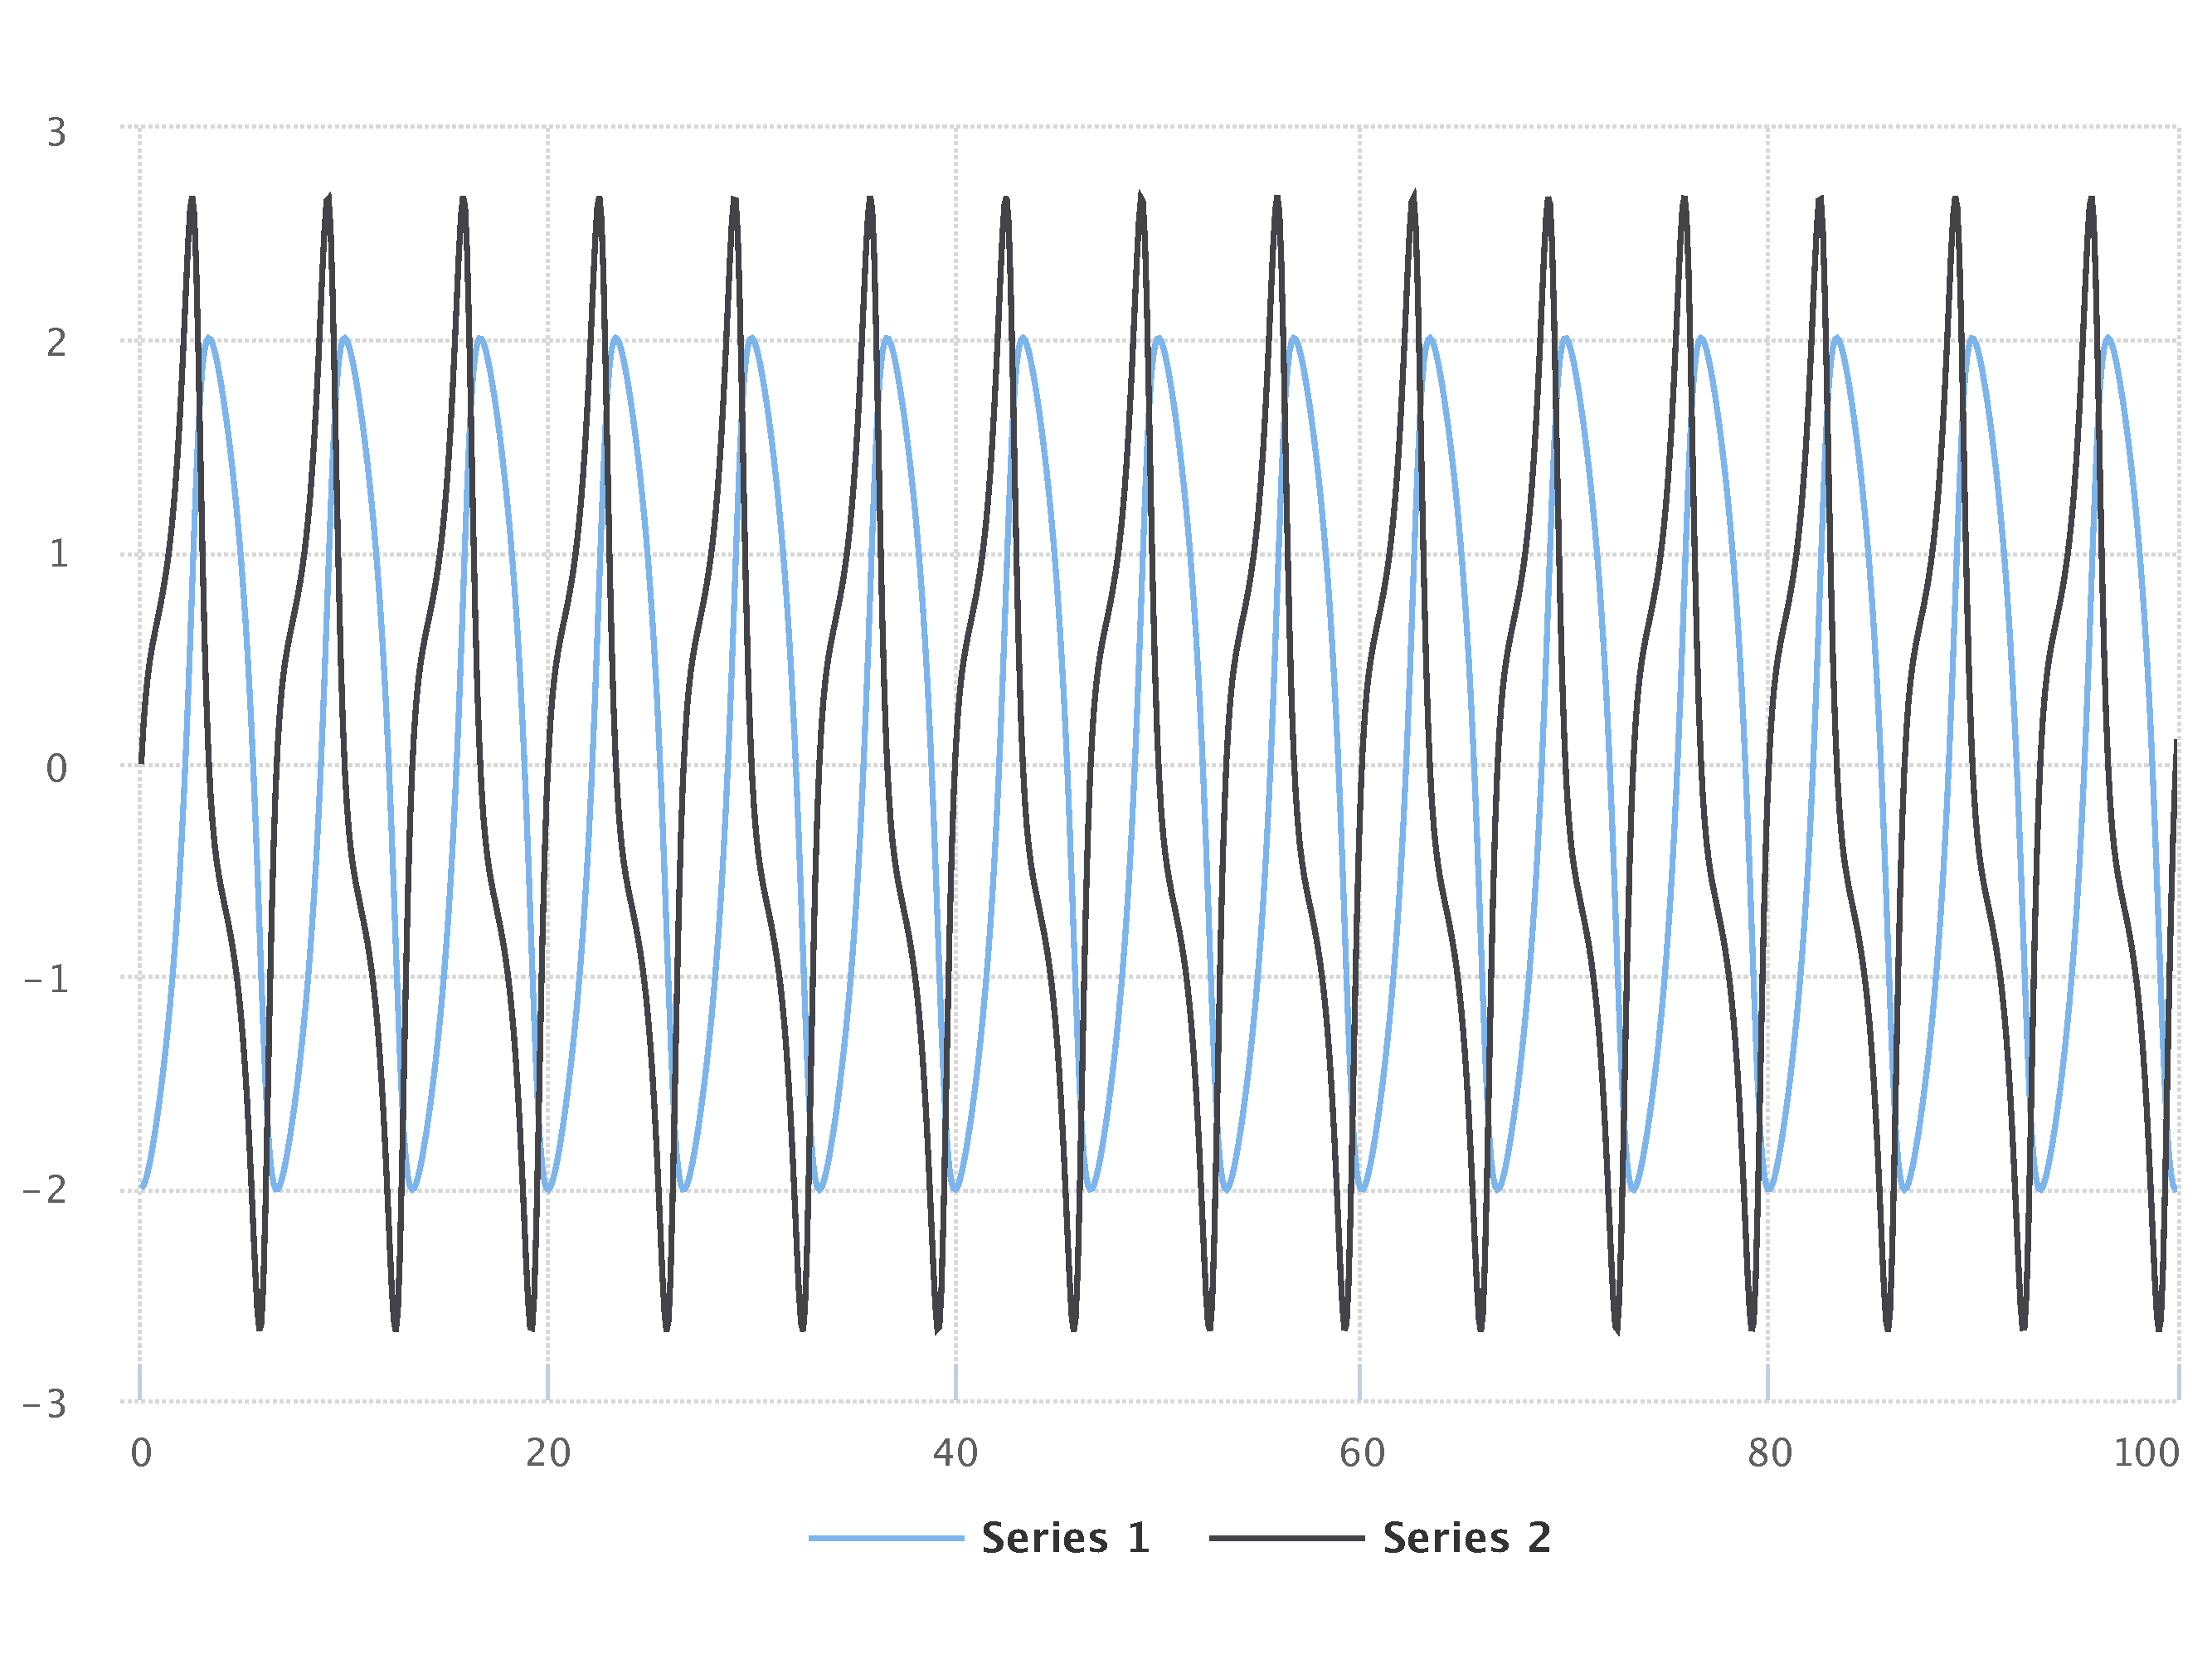
\includegraphics[width=1.0\textwidth]{examples/vanderpol-sbml/results/sedml_webtools/plot1}
        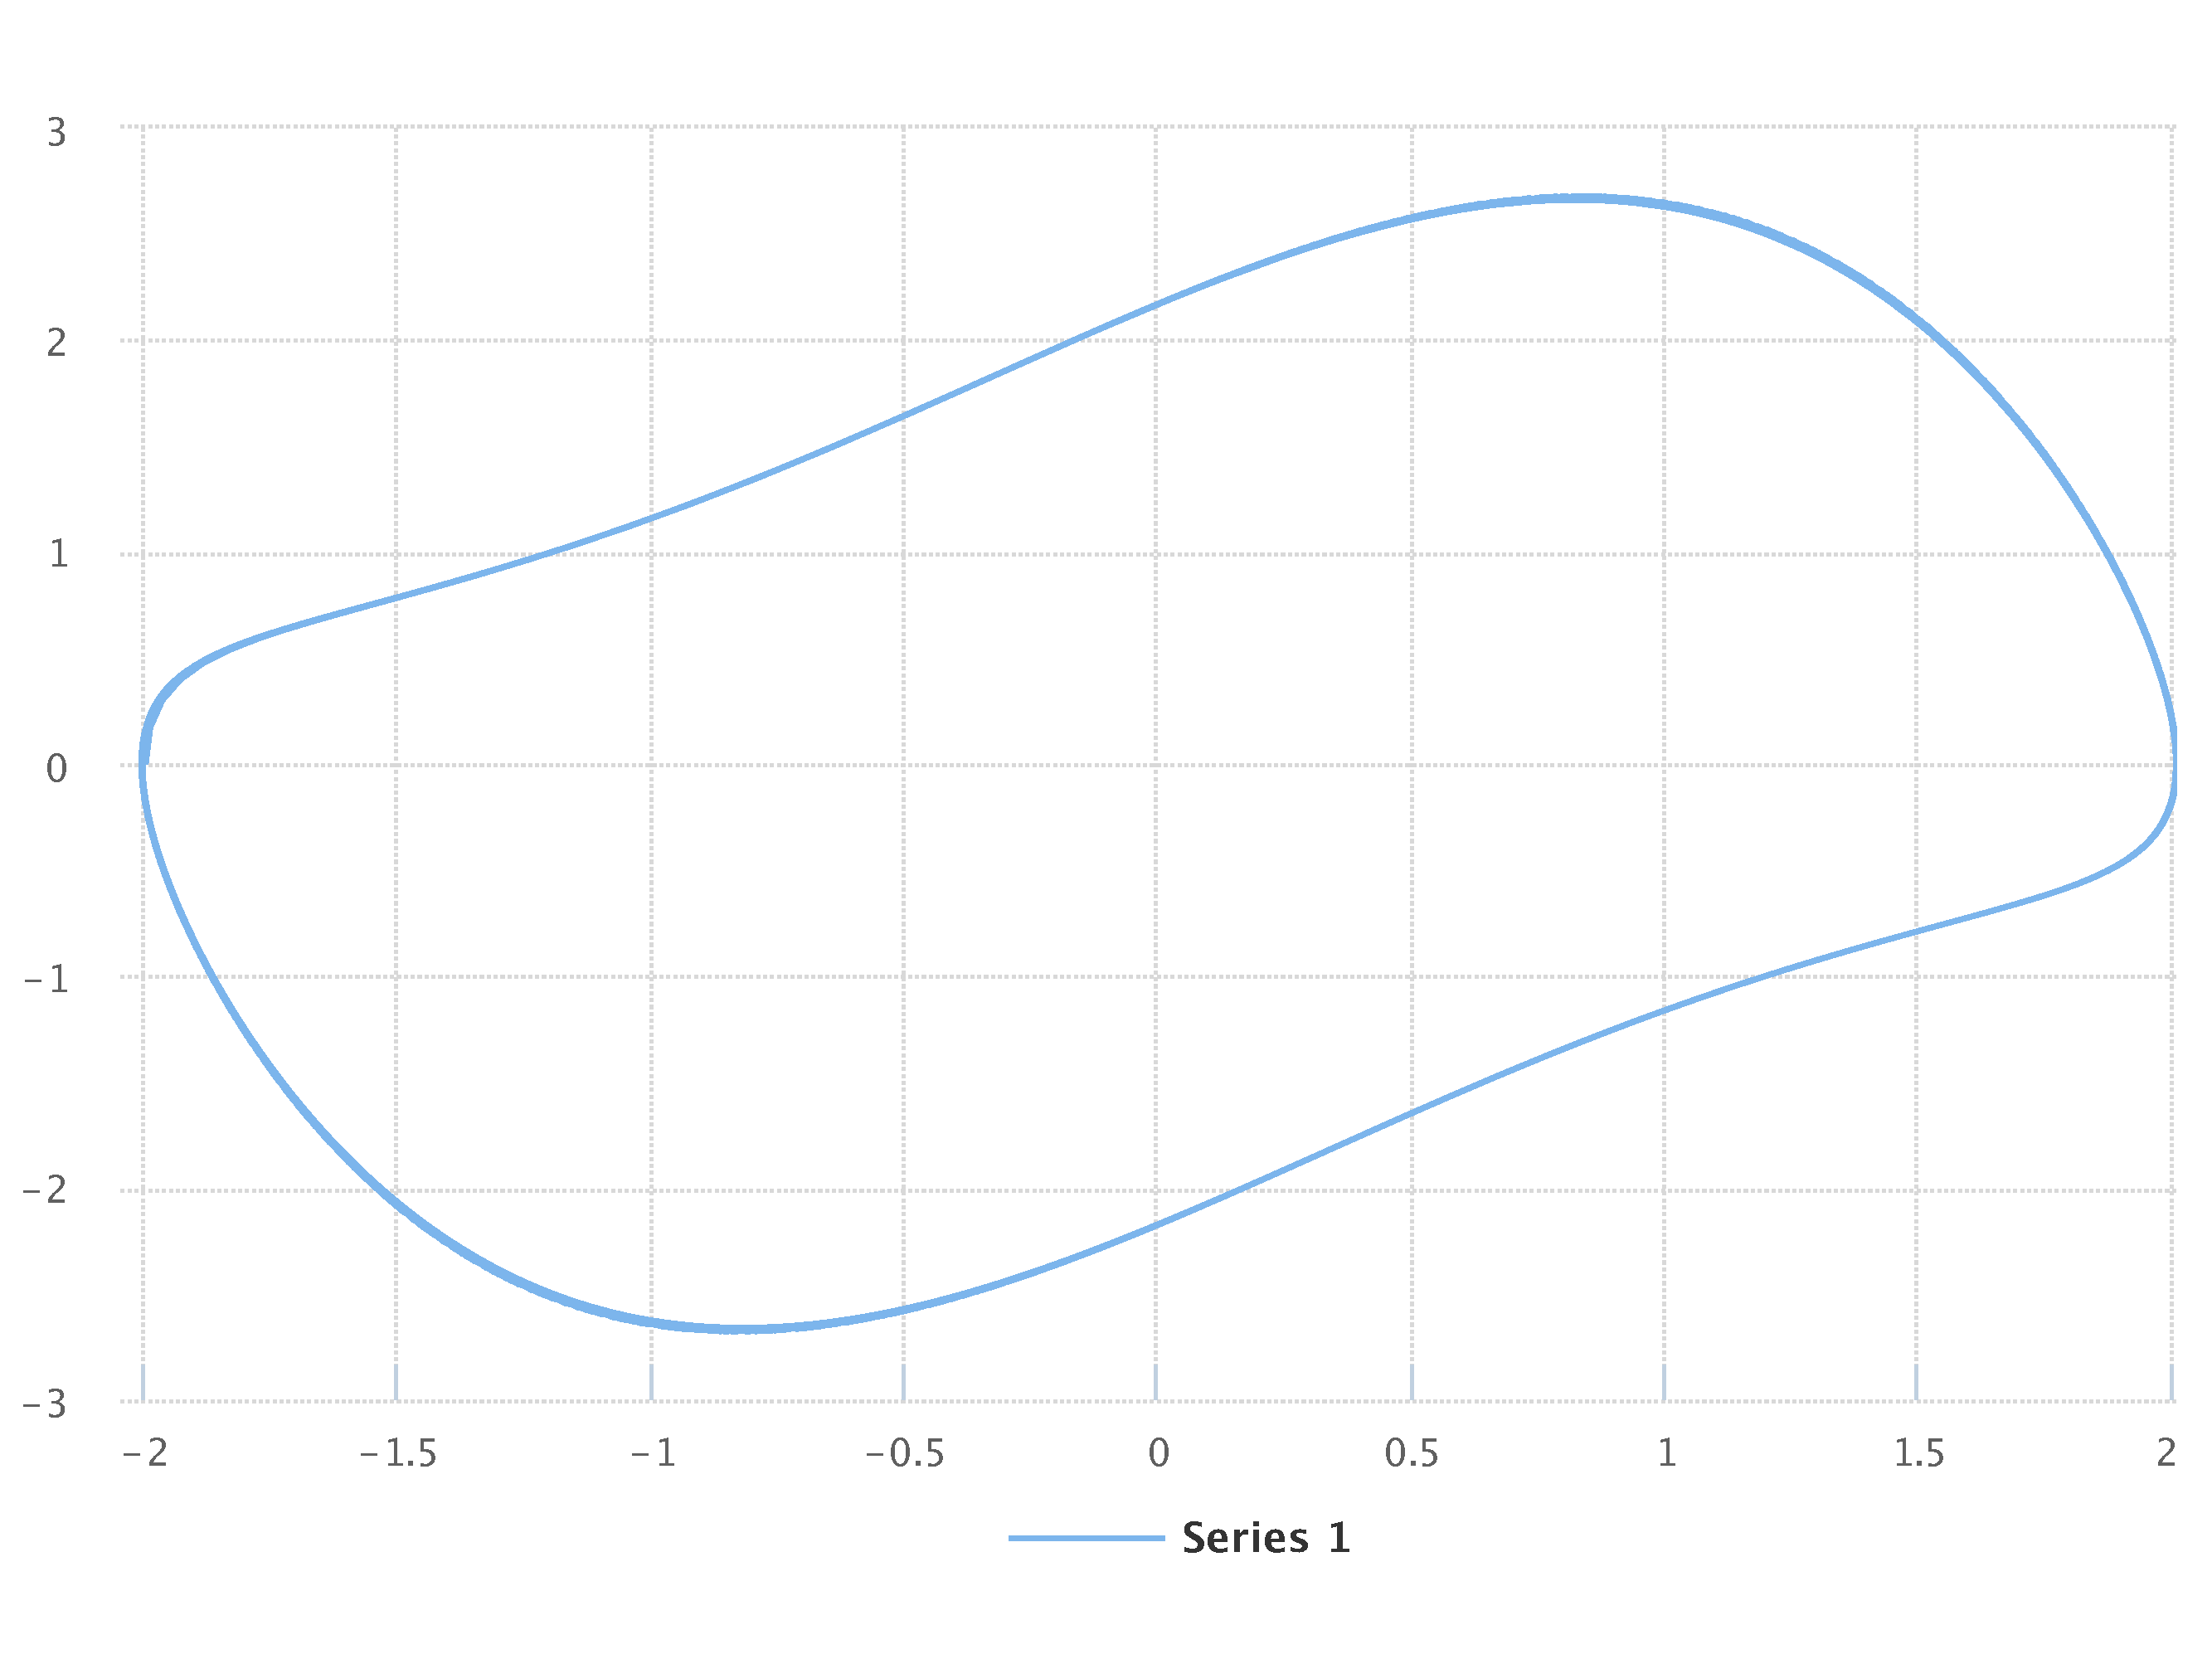
\includegraphics[width=1.0\textwidth]{examples/vanderpol-sbml/results/sedml_webtools/plot2}
        \caption{The simulation result gained from the simulation description given in \lst{vanderpol-sbml}. Simulation with SED-ML web tools \citep{bergmann2017sed}.}
    \end{minipage}\hfill
    \begin{minipage}{0.47\textwidth}
        \centering
        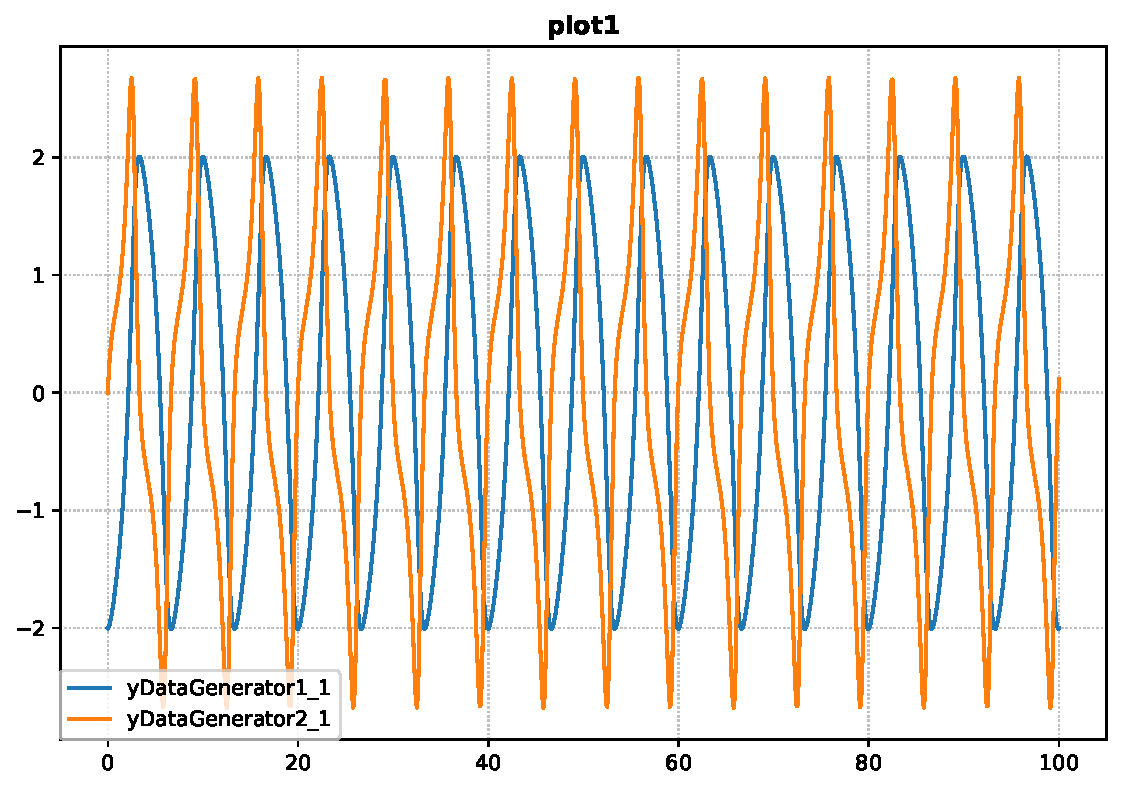
\includegraphics[width=1.0\textwidth]{examples/vanderpol-sbml/results/tellurium/plot1}
        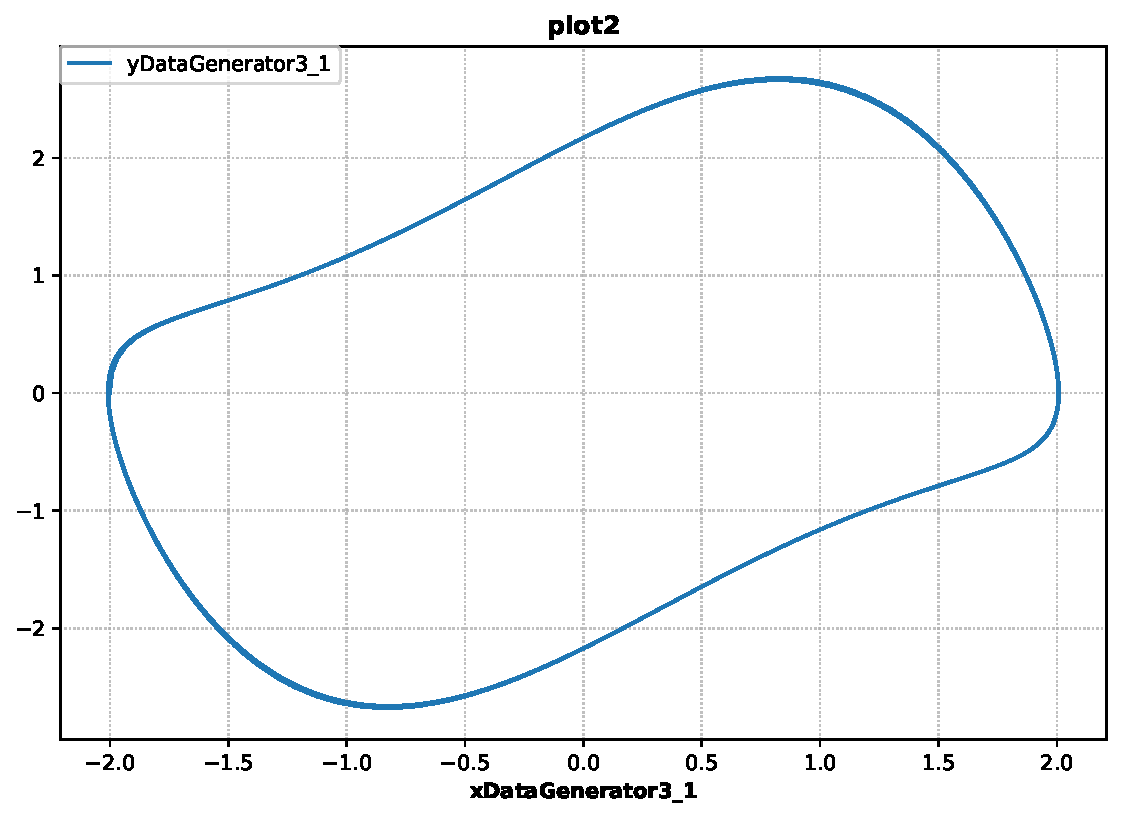
\includegraphics[width=1.0\textwidth]{examples/vanderpol-sbml/results/tellurium/plot2}
        \caption{Simulation with tellurium \citep{tellurium}.}
    \end{minipage}
    \label{fig:lorenz-sbml}
\end{figure}

\myXmlImport{Van der Pol Model (SBML) Simulation Description in SED-ML}{lst:vanderpol-sbml}{examples/vanderpol-sbml/vanderpol.xml}

\subsection{Van der Pol Model in CellML (\texttt{L1V3\_vanderpol-cellml.omex})}
\label{example:vanderpol_cellml}
The following example provides a SED-ML description for the simulation of the Van der Pol model in CellML \citep{cuellar:2003}. The time-course and the behavior in the phase plane are plotted. The mathematical model and the performed simulation experiment are identical to Appendix~\ref{example:vanderpol_sbml}.

\begin{figure}[ht]
    \centering
    \begin{minipage}{0.47\textwidth}
        \centering
        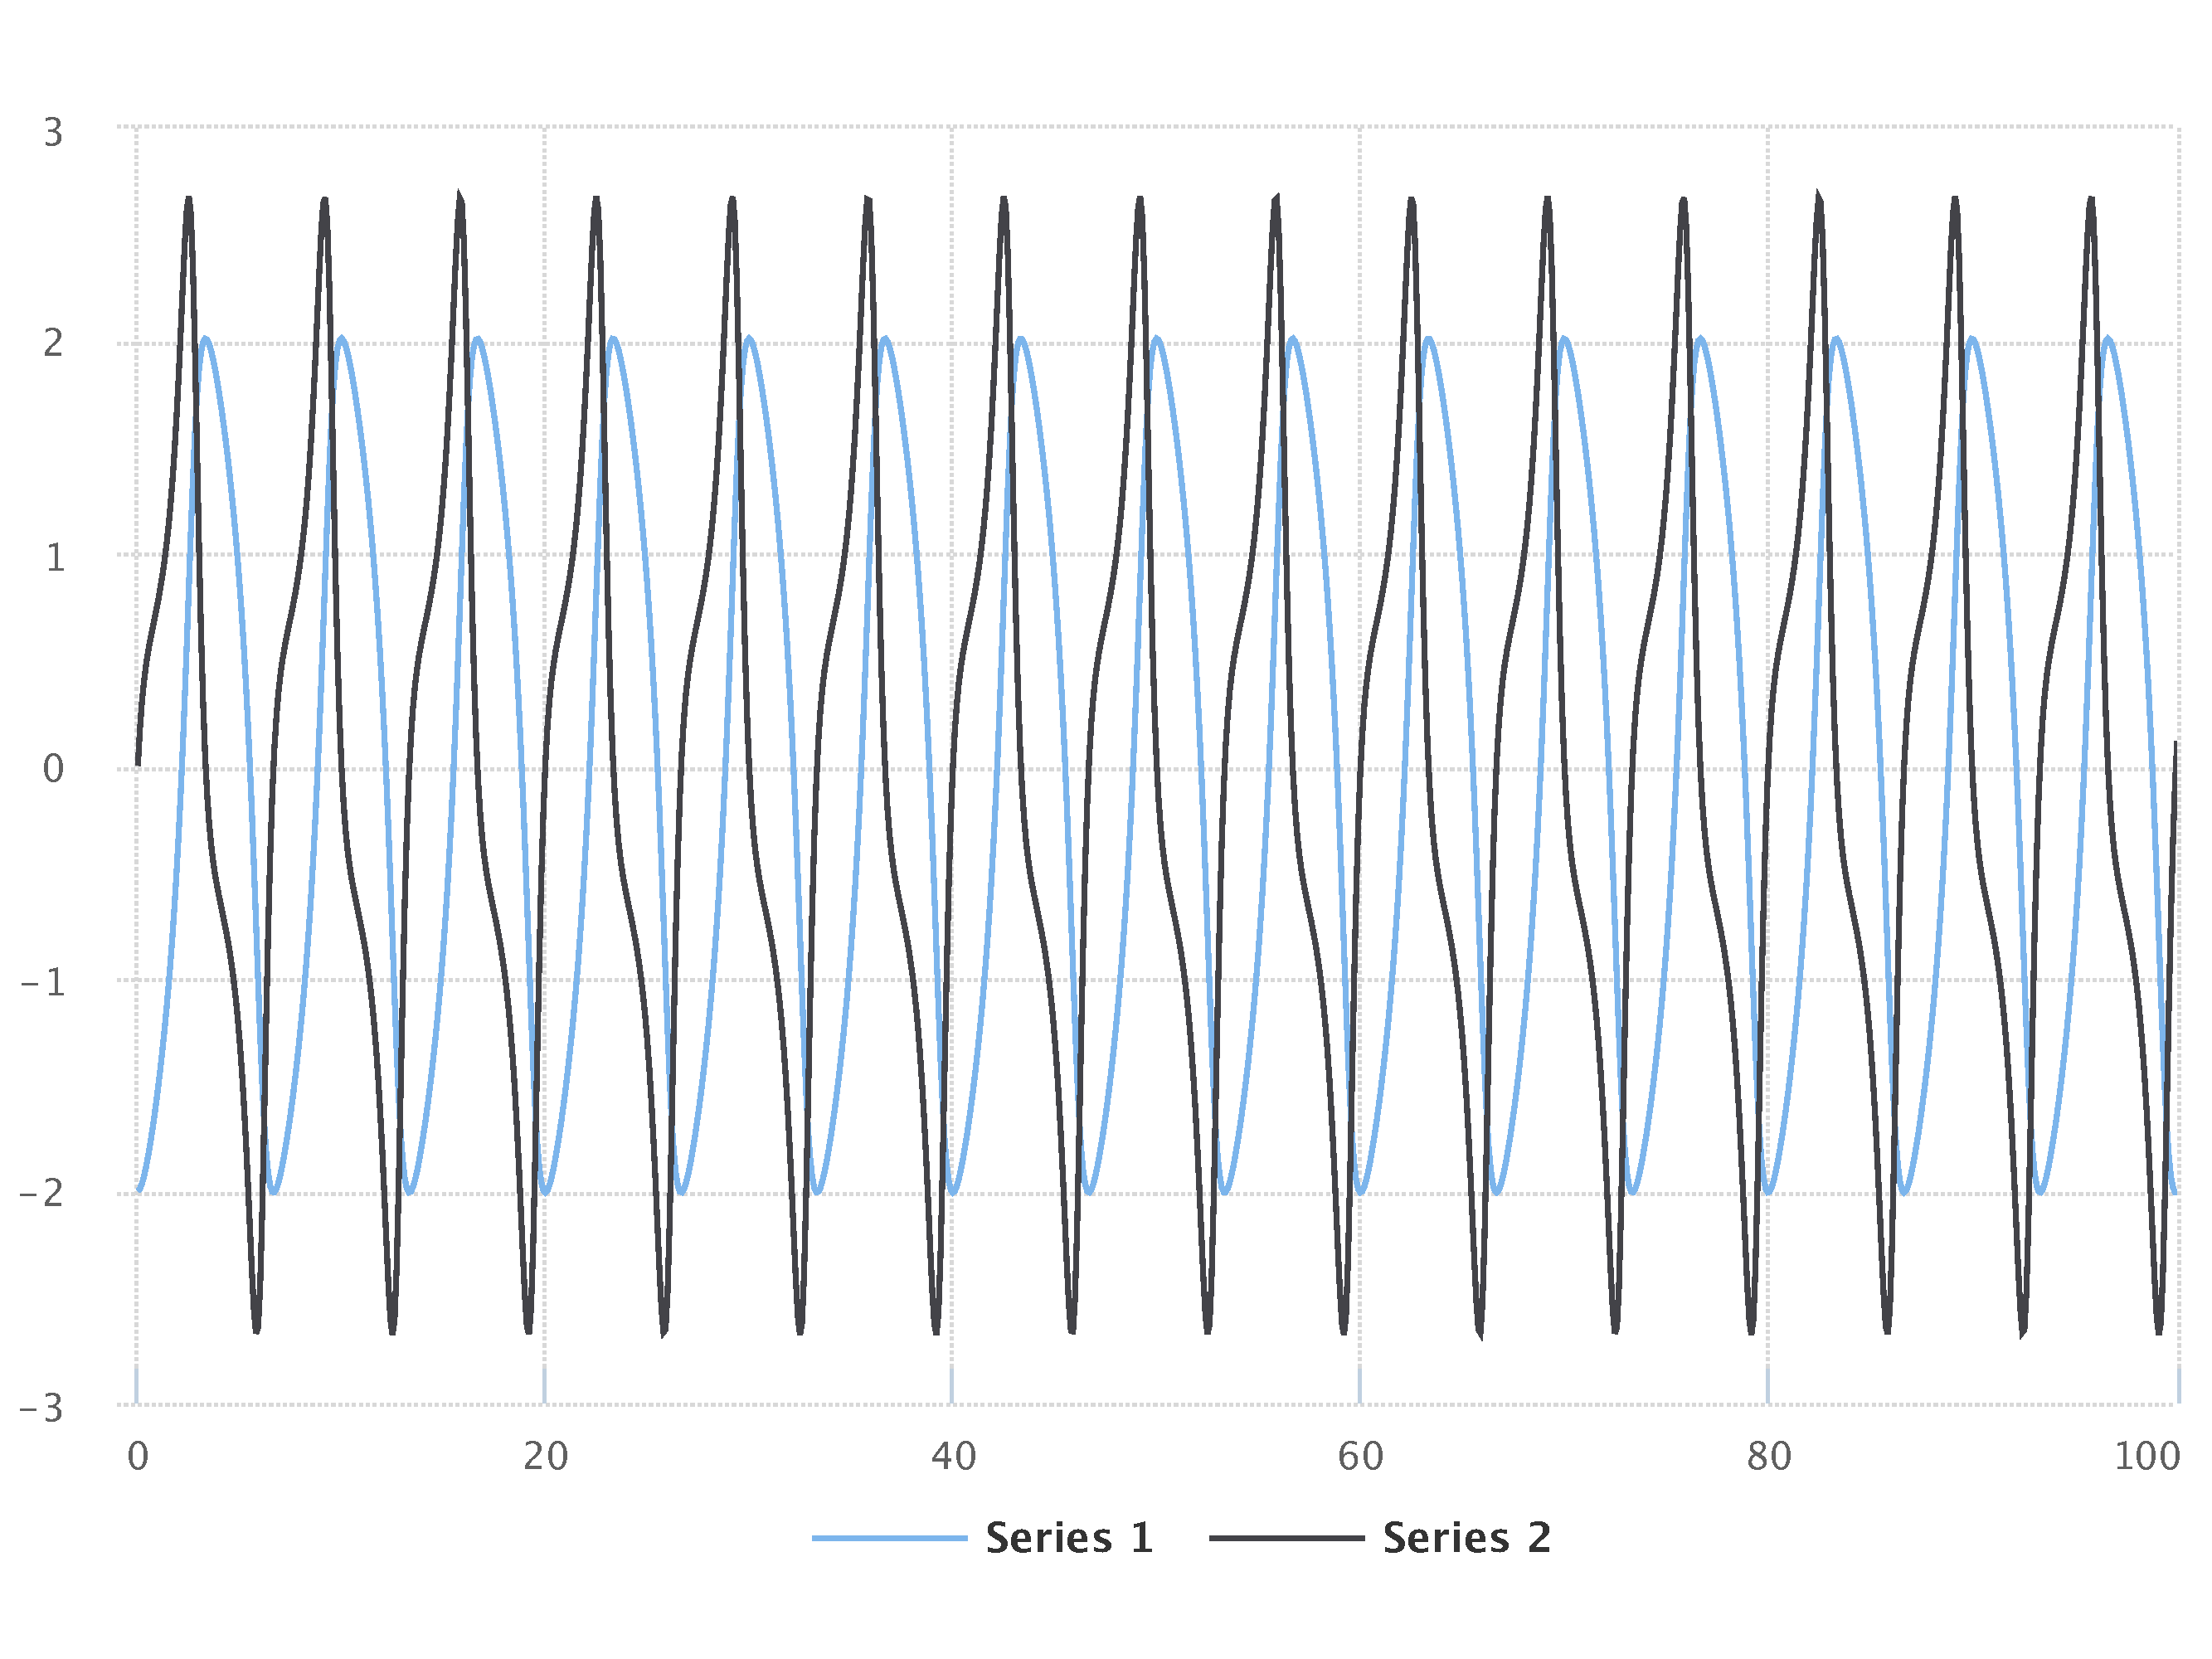
\includegraphics[width=1.0\textwidth]{examples/vanderpol-cellml/results/sedml_webtools/plot1}
        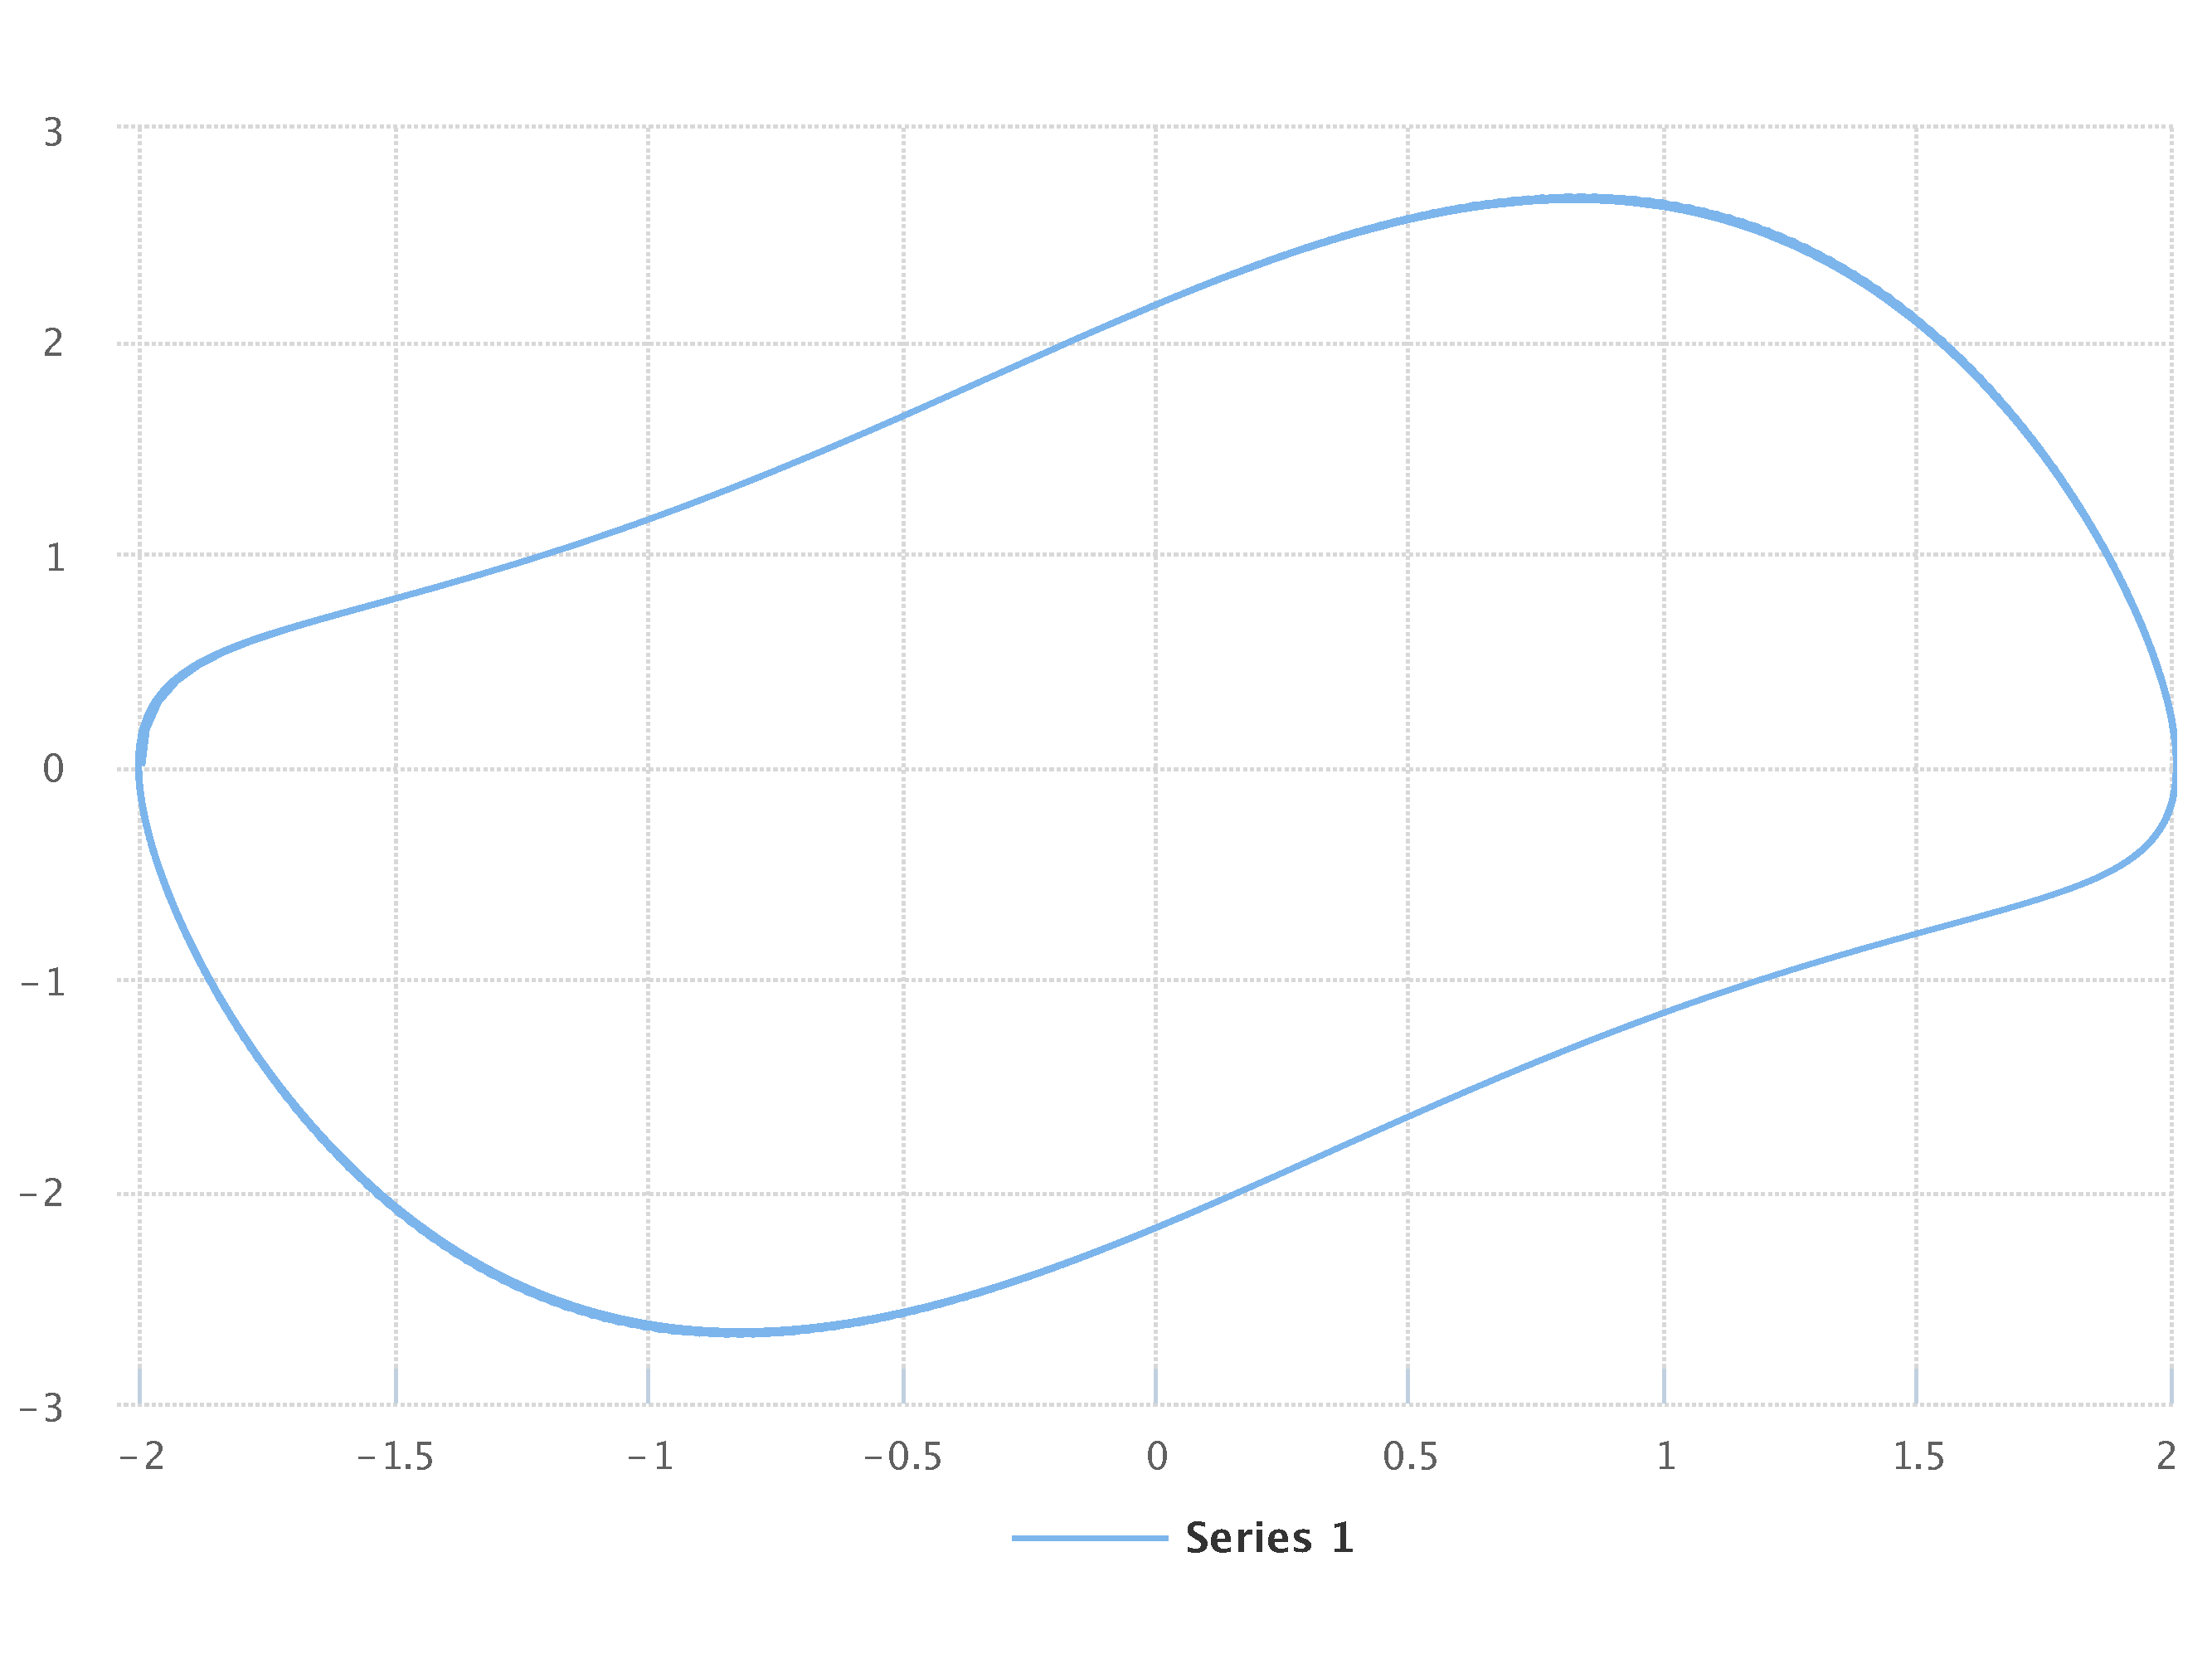
\includegraphics[width=1.0\textwidth]{examples/vanderpol-cellml/results/sedml_webtools/plot2}
        \caption{The simulation result gained from the simulation description given in \lst{vanderpol-cellml}. Simulation with SED-ML web tools \citep{bergmann2017sed}.}
    \end{minipage}\hfill
    \begin{minipage}{0.5\textwidth}
        \centering
        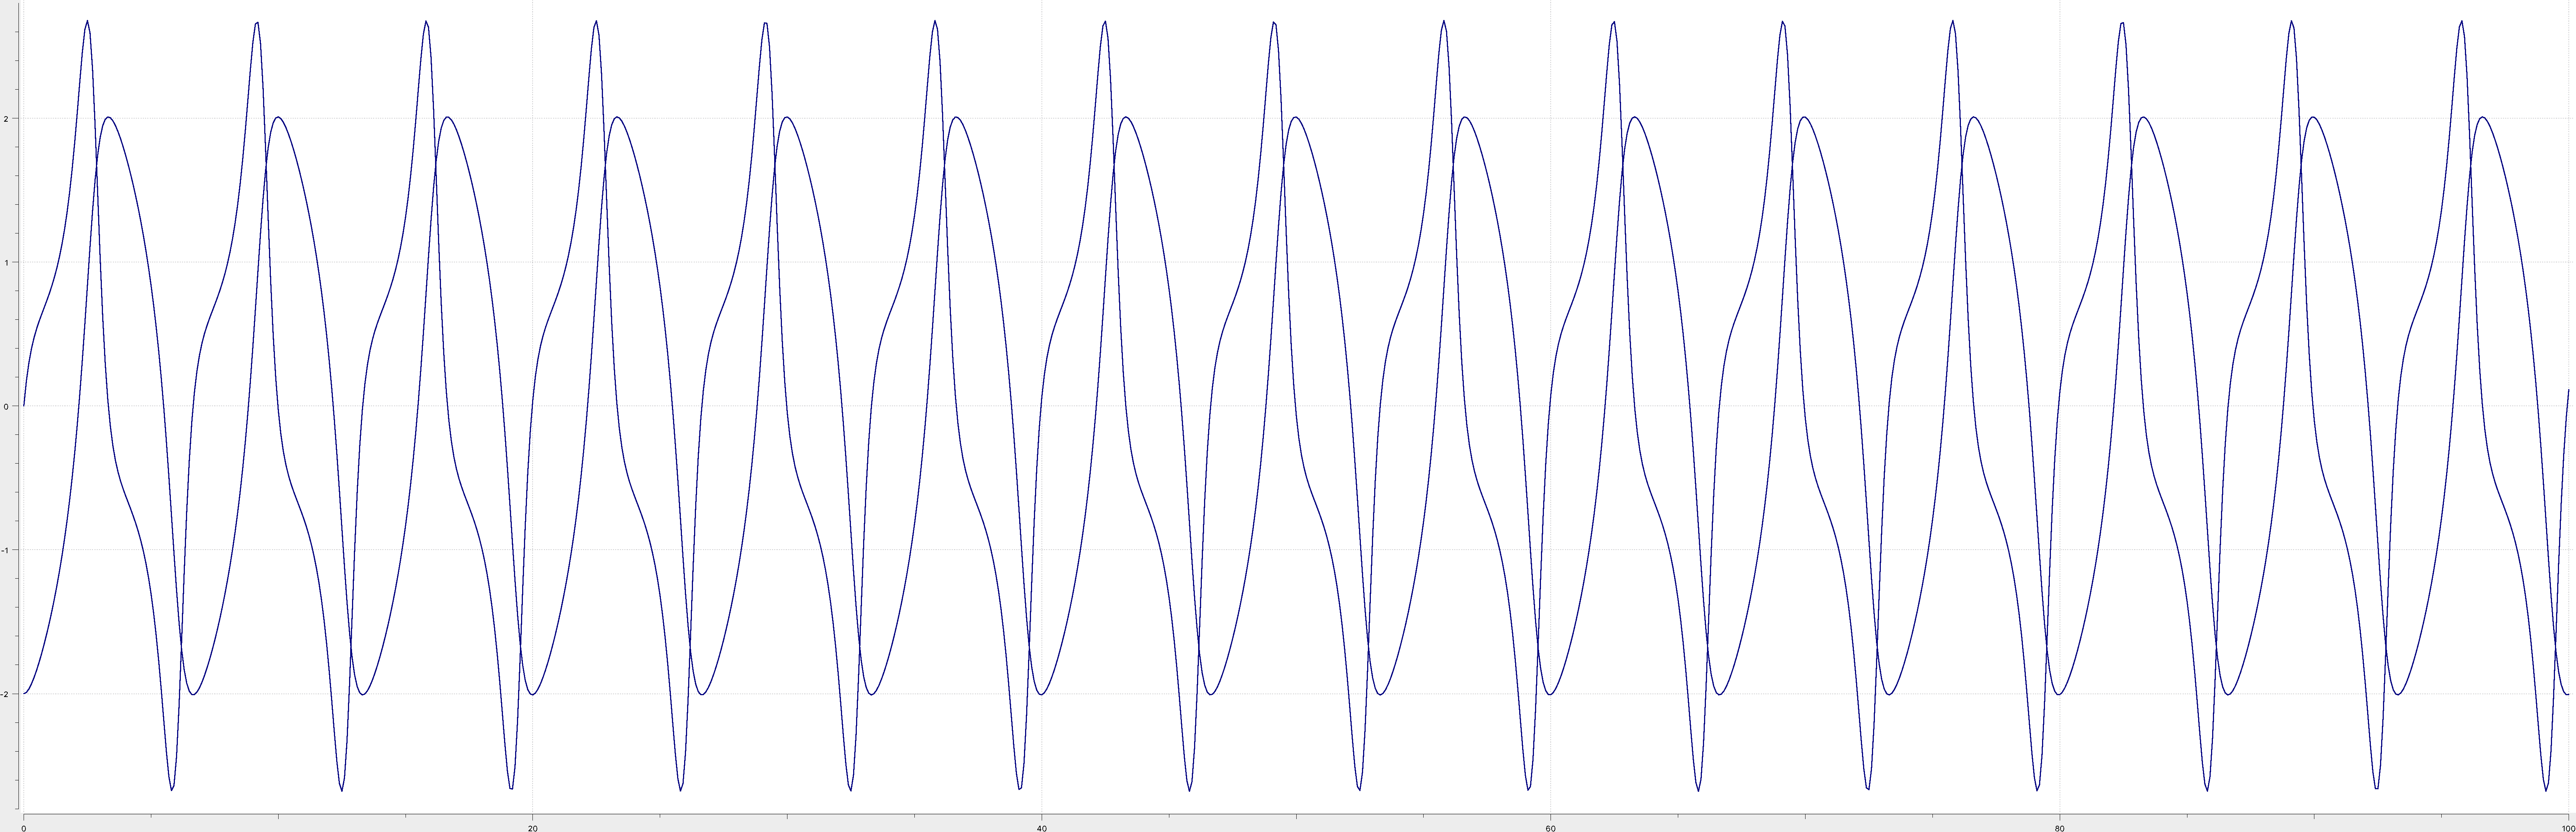
\includegraphics[width=1.0\textwidth]{examples/vanderpol-cellml/results/opencor/plot1}
        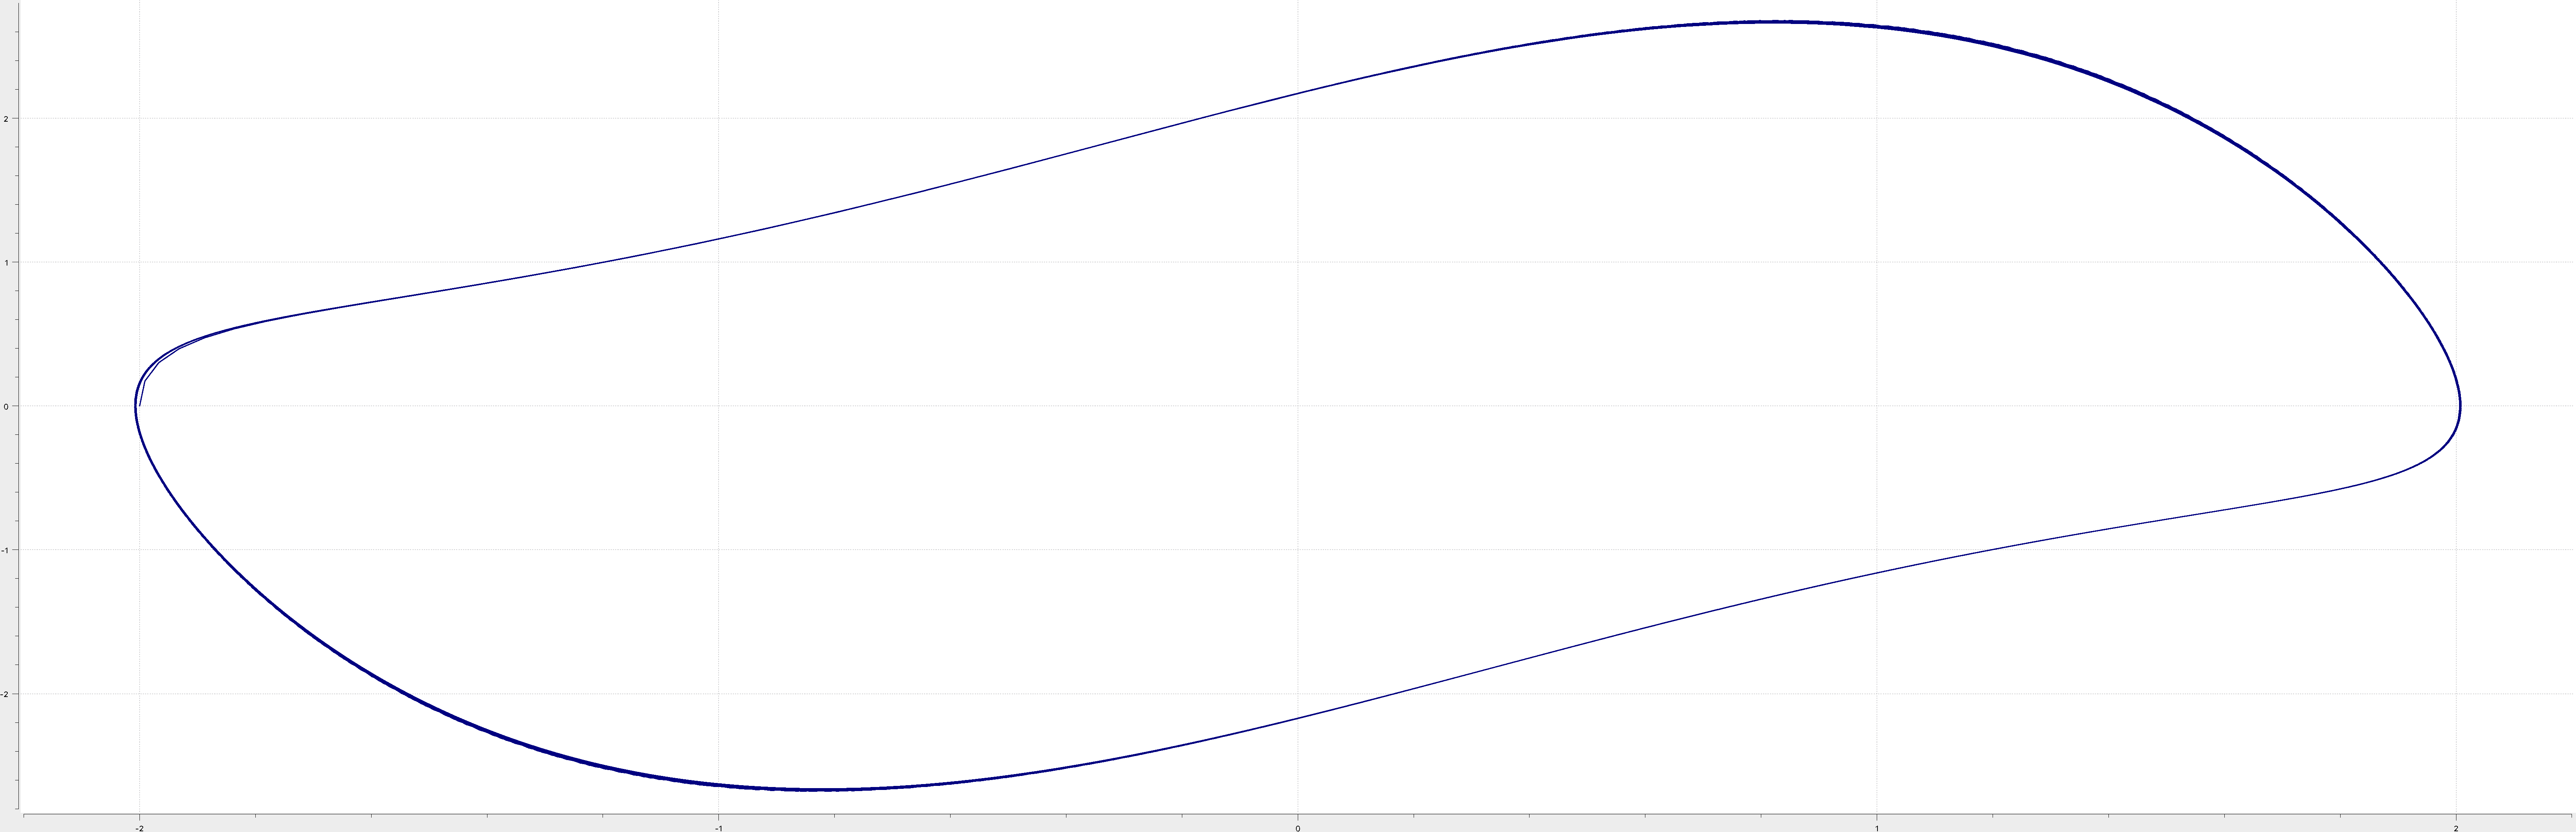
\includegraphics[width=1.0\textwidth]{examples/vanderpol-cellml/results/opencor/plot2}
        \caption{Simulation with OpenCOR \citep{garny2015opencor}.}
    \end{minipage}
    \label{fig:lorenz-cellml}
\end{figure}

\myXmlImport{Van der Pol Model (CellML) Simulation Description in SED-ML}{lst:vanderpol-cellml}{examples/vanderpol-cellml/vanderpol.xml}

% LORENZ EXAMPLES - DETERMINISTIC CHAOS
%\subsection{Lorenz Model SBML (\code{lorenz-sbml.omex})}
%\label{example:lorenz_sbml}
%The following example provides a SED-ML description for the simulation of the Lorenz model in SBML.
%
%\begin{figure}[ht]
%    \centering
%    \begin{minipage}{0.47\textwidth}
%        \centering
%        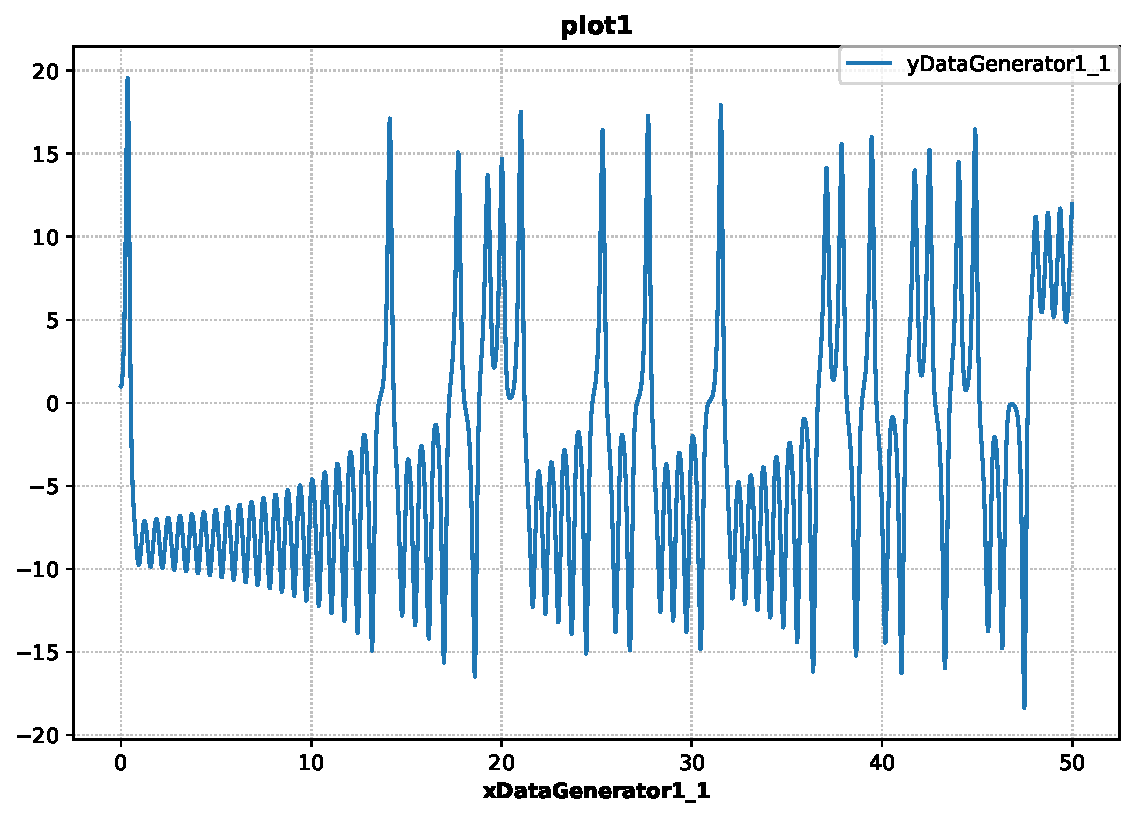
\includegraphics[width=1.0\textwidth]{examples/lorenz-sbml/results/sedml_webtools/plot1}
%        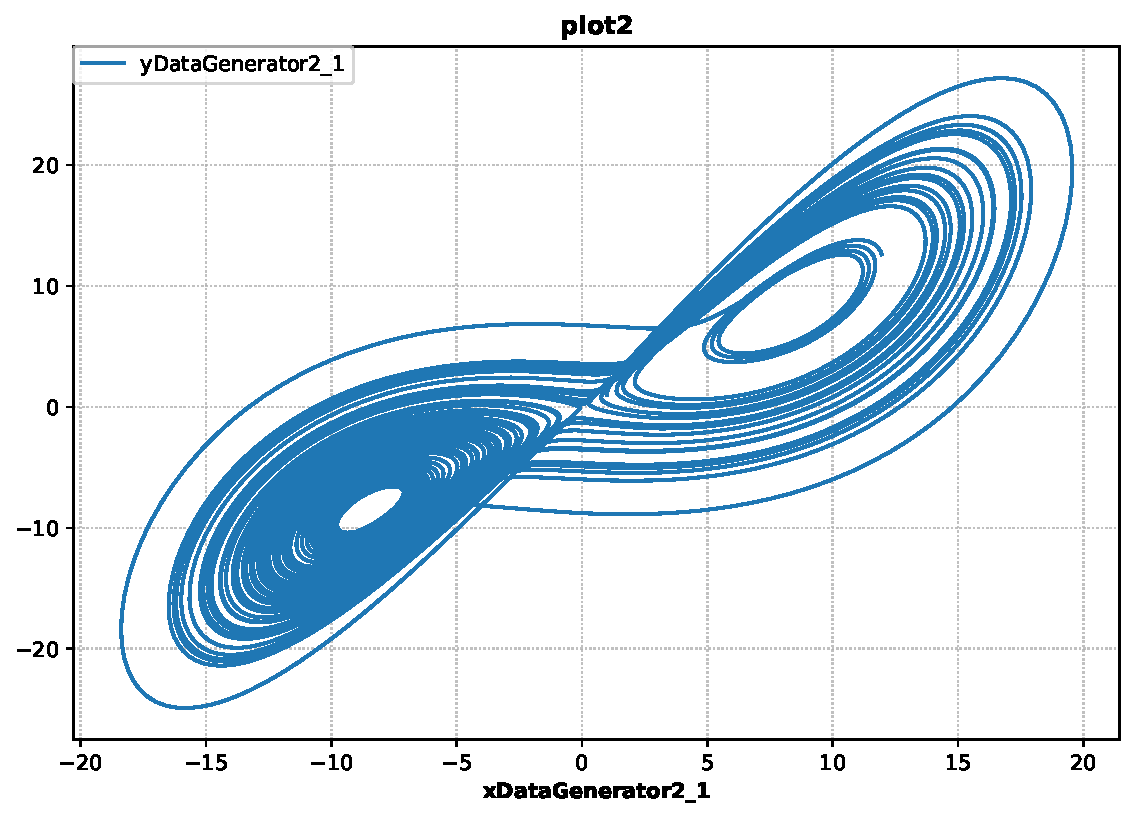
\includegraphics[width=1.0\textwidth]{examples/lorenz-sbml/results/sedml_webtools/plot2}
%		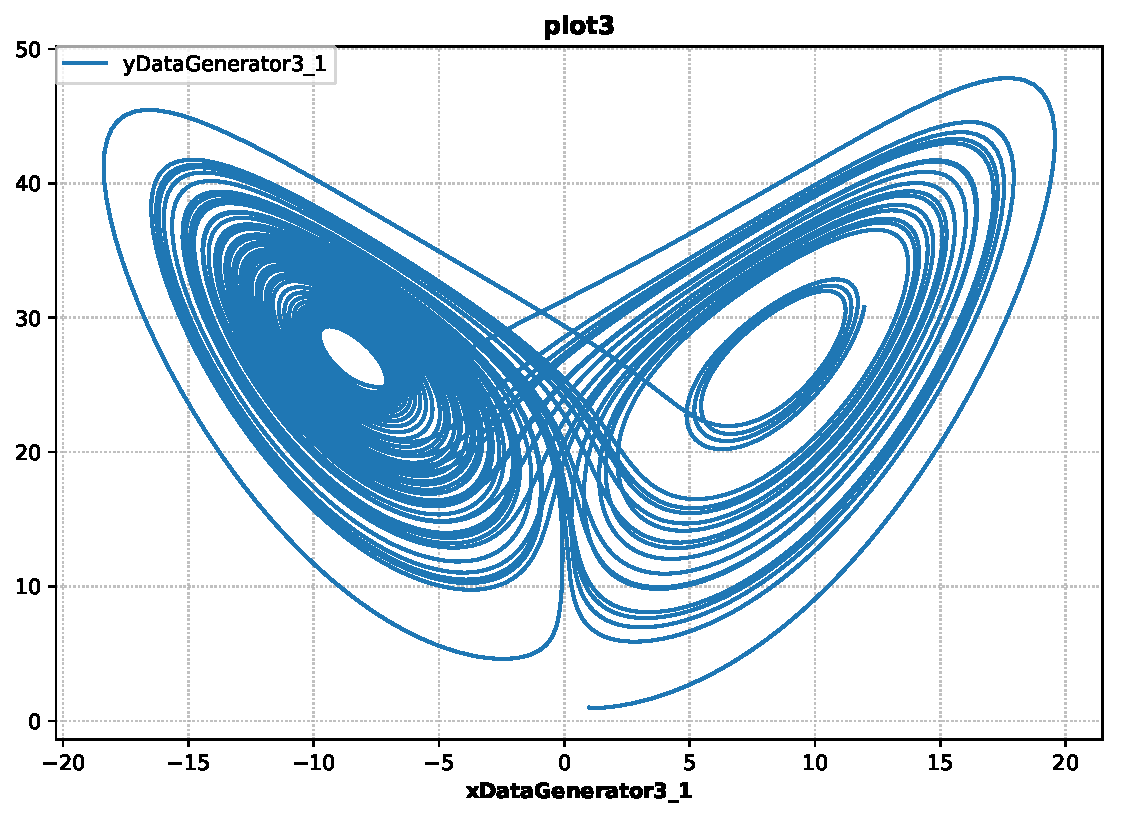
\includegraphics[width=1.0\textwidth]{examples/lorenz-sbml/results/sedml_webtools/plot3}
%        \caption{The simulation result gained from the simulation description given in \lst{lorenz-sbml}. Simulation with SED-ML web tools \citep{bergmann2017sed}.}
%    \end{minipage}\hfill
%    \begin{minipage}{0.47\textwidth}
%        \centering
%        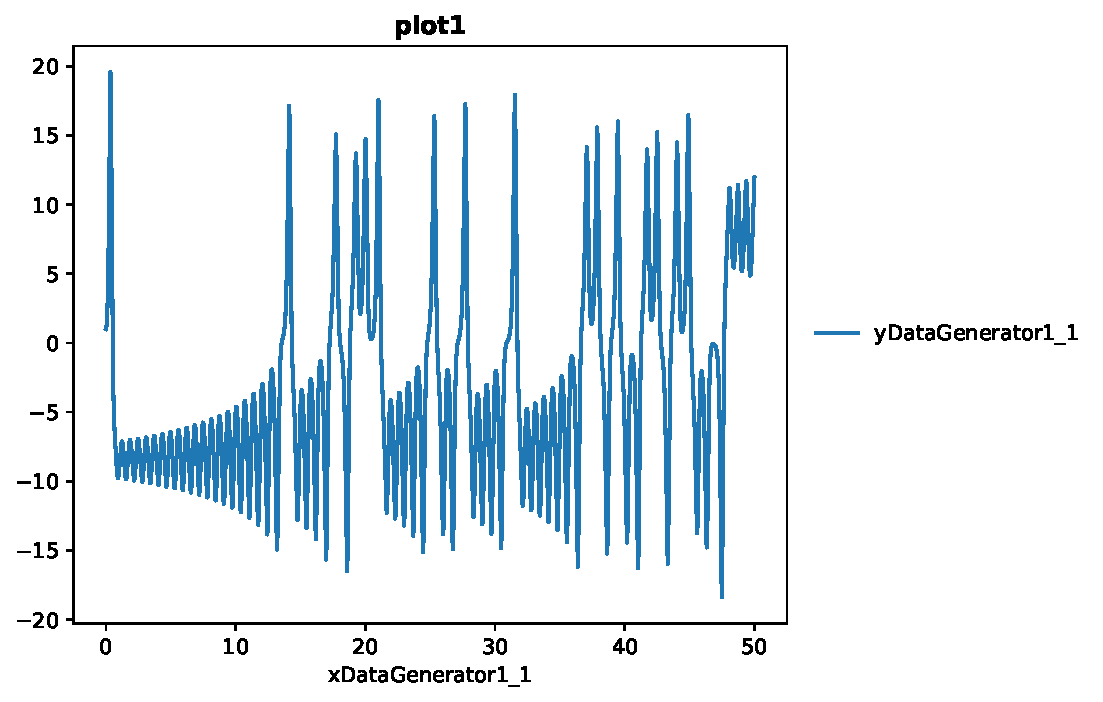
\includegraphics[width=1.0\textwidth]{examples/lorenz-sbml/results/tellurium/plot1}
%        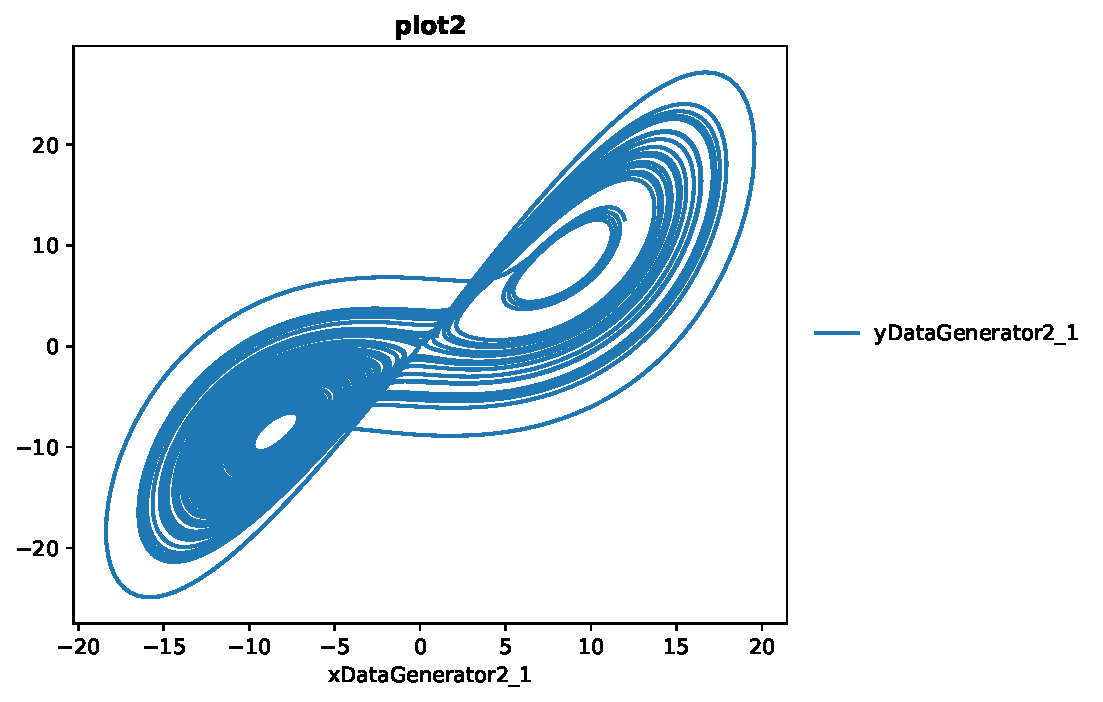
\includegraphics[width=1.0\textwidth]{examples/lorenz-sbml/results/tellurium/plot2}
%		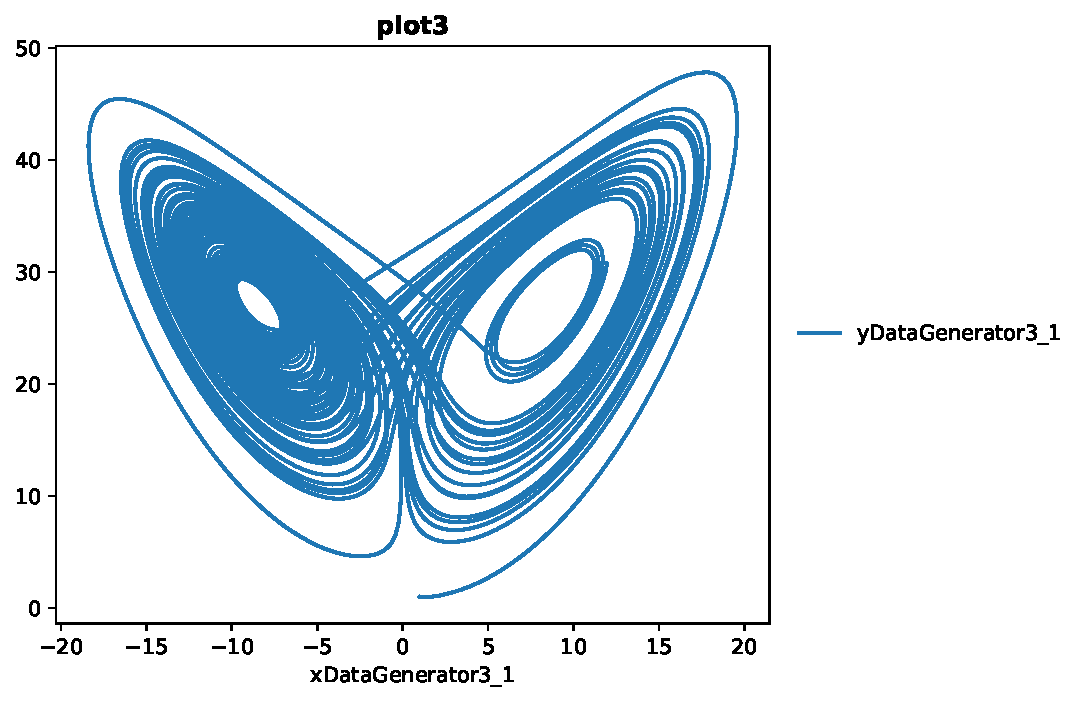
\includegraphics[width=1.0\textwidth]{examples/lorenz-sbml/results/tellurium/plot3}
%        \caption{Simulation with tellurium \citep{tellurium}.}
%    \end{minipage}
%    \label{fig:lorenz-sbml}
%\end{figure}
%
%\myXmlImport{LeLoup Model Simulation Description in SED-ML}{lst:lorenz-sbml}{examples/lorenz-sbml/lorenz.xml}
%
%\subsection{Lorenz Model CellML (\code{lorenz-cellml.omex})}
%\label{example:lorenz_cellml}
%The following example provides a SED-ML description for the simulation of the Lorenz model in CellML.
%
%\begin{figure}[ht]
%    \centering
%    \begin{minipage}{0.47\textwidth}
%        \centering
%        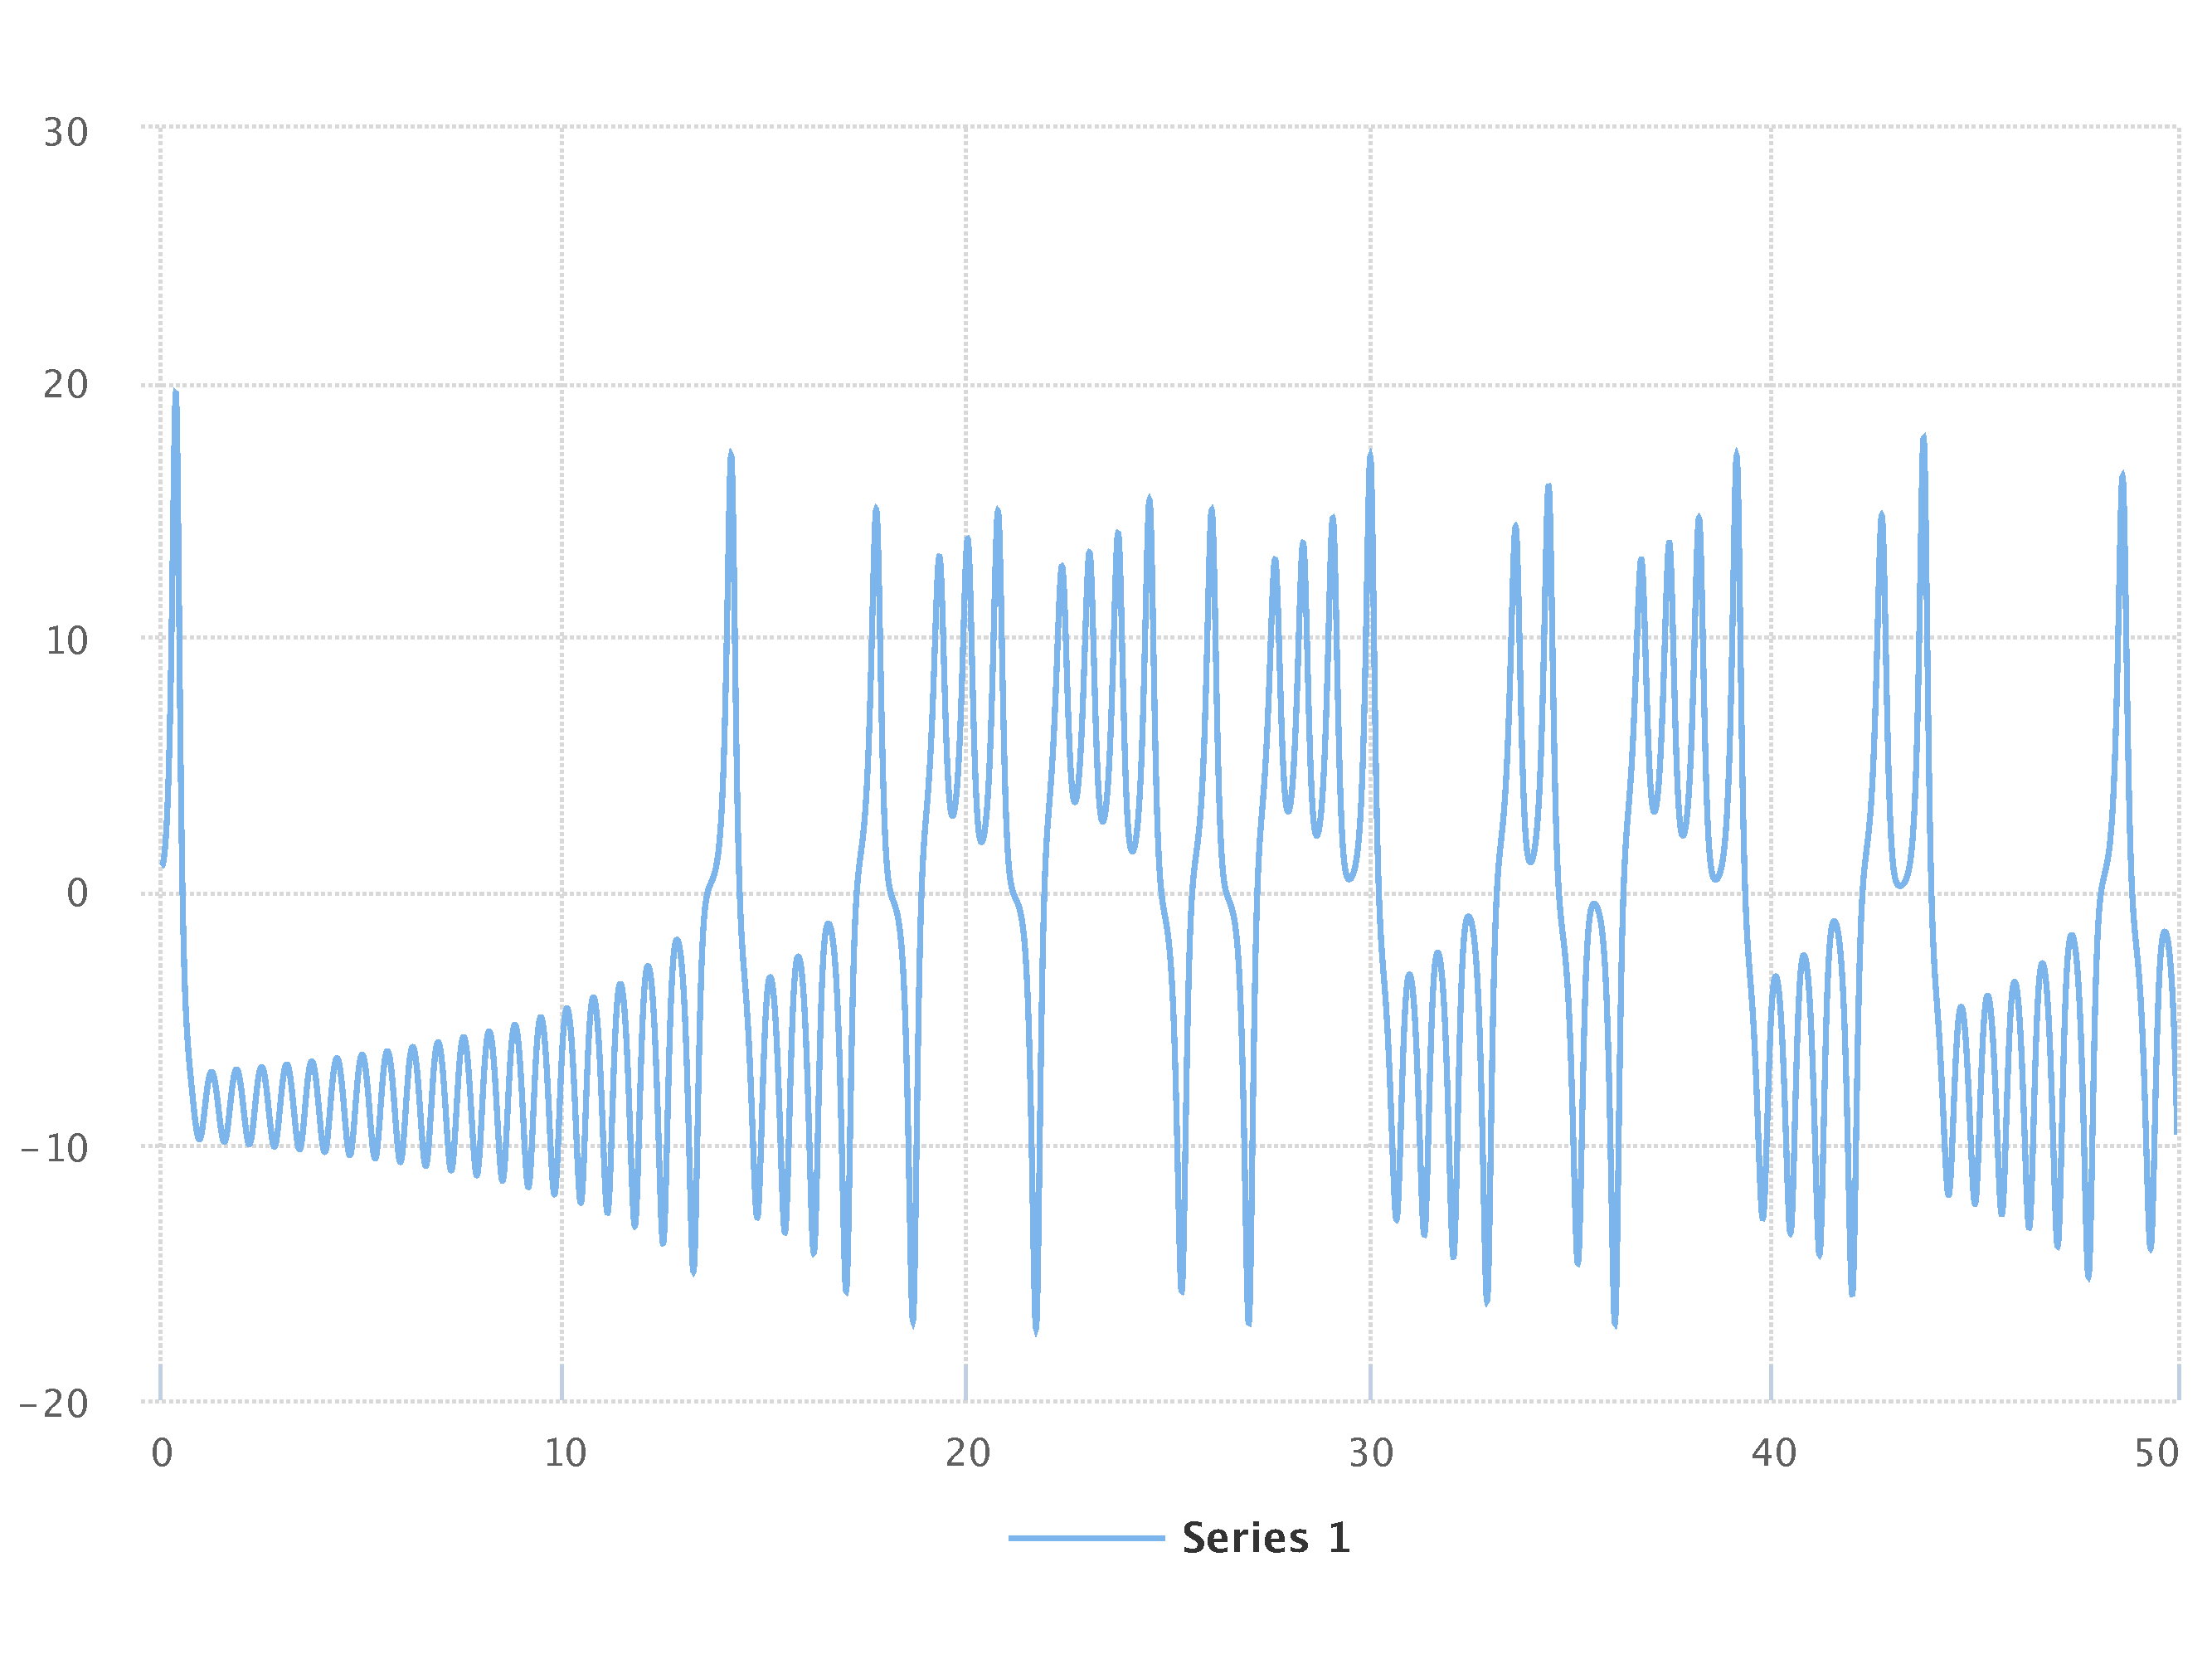
\includegraphics[width=1.0\textwidth]{examples/lorenz-cellml/results/sedml_webtools/plot1}
%        \caption{The simulation result gained from the simulation description given in \lst{lorenz-cellml}. Simulation with SED-ML web tools \citep{bergmann2017sed}.}
%    \end{minipage}\hfill
%    \begin{minipage}{0.47\textwidth}
%        \centering
%        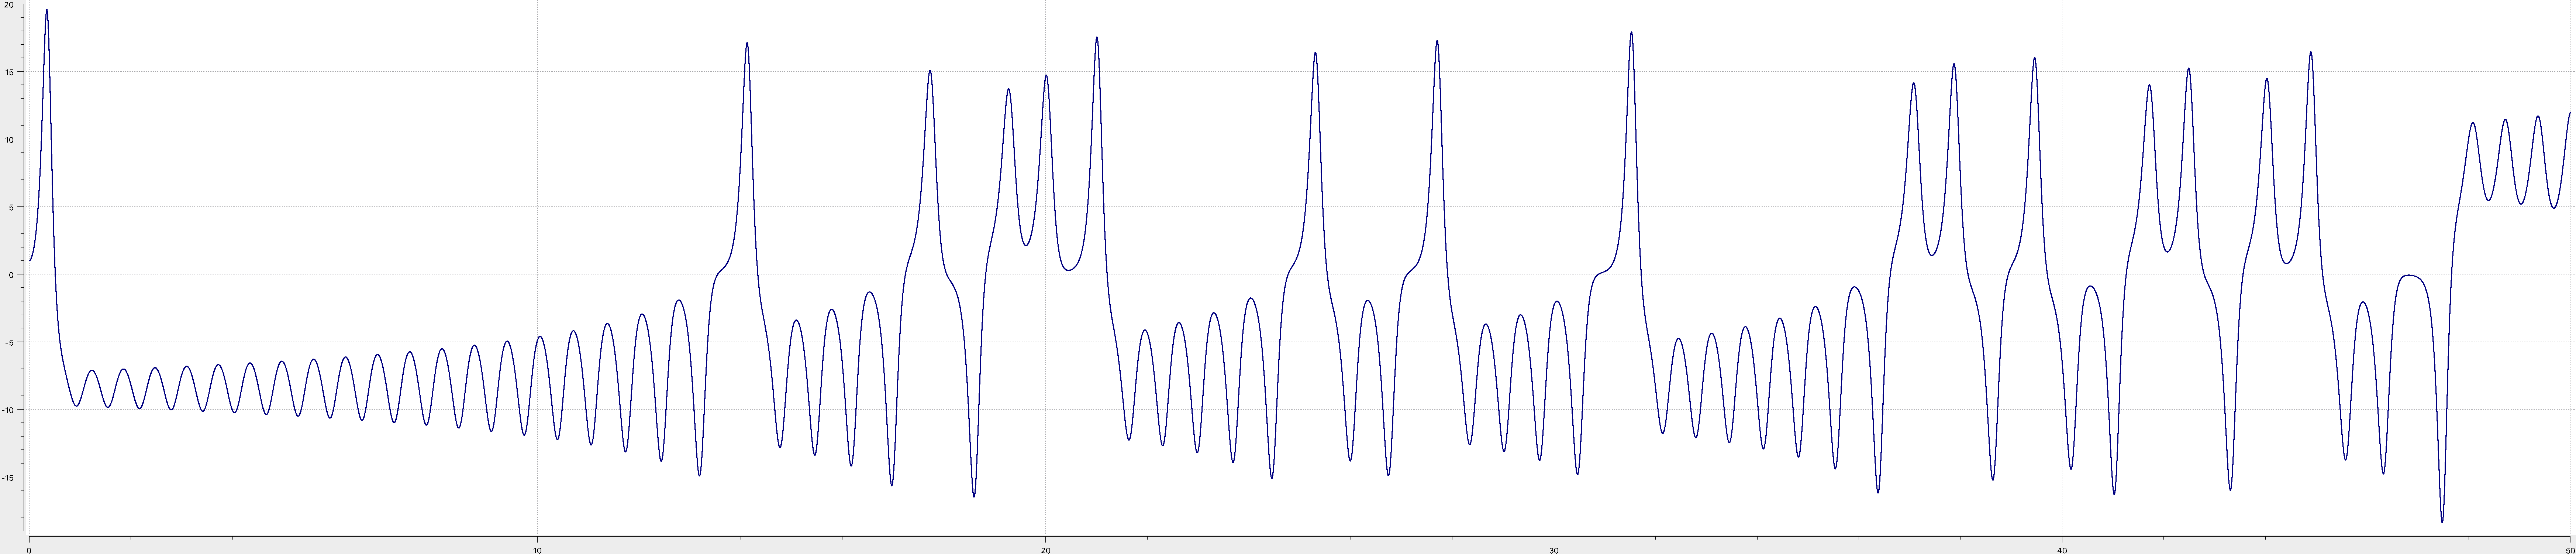
\includegraphics[width=1.0\textwidth]{examples/lorenz-cellml/results/opencor/plot1}
%        \caption{Simulation with OpenCOR \citep{garny2015opencor}.}
%    \end{minipage}
%    \label{fig:lorenz-cellml}
%\end{figure}
%
%\myXmlImport{LeLoup Model Simulation Description in SED-ML}{lst:lorenz-cellml}{examples/lorenz-cellml/lorenz.xml}

\pagebreak
% ~~~~~~~~~~~~~~~~~~~~~~~~~~~~~~~~~~~~
% REPRODUCING PUBLICATION RESULTS
% ~~~~~~~~~~~~~~~~~~~~~~~~~~~~~~~~~~~~
\section{Reproducing publication results}
SED-ML allows to describe simulation experiments from publications in a reproducible manner. This section provides such examples.

% ~~~ LE LOUP (SBML) ~~~
\subsection{Le Loup Model (\texttt{L1V3\_leloup-sbml.omex})}
\label{example:leloup_sbml}
The following example provides a SED-ML description for the simulation of the model based on the publication \cite{LeLoup1999}.

The model is referenced by its SED-ML \hyperref[sec:id]{\element{id}} \code{model1} and refers to the model with the MIRIAM URN \url{urn:miriam:biomodels.db:BIOMD0000000021}. A second model is defined in the example, using \code{model1} as a source and applying additional changes to it, in this case updating two model parameters.

One simulation setup is defined in the \code{listOfSimulations}. It is a \code{uniformTimeCourse} over 380 time units, providing 1000 output points. The algorithm used is the CVODE solver, as denoted by the KiSAO ID \code{KiSAO:0000019}.

A number of \hyperref[class:dataGenerator]{dataGenerators} are defined, which are the prerequisite for defining the simulation \hyperref[class:output]{output}. The first \hyperref[class:dataGenerator]{dataGenerator} with \hyperref[sec:id]{\element{id}} \code{time} collects the simulation time. \code{tim1} maps on the \code{Mt} entity in the model that is used in \code{task1} which in the model \code{model1}. The dataGenerator named \code{\texttt{per\_tim1}} maps on the \code{Cn} entity in \code{model1}. Finally  the fourth and fifth dataGenerators map on the \code{Mt} and \code{\texttt{per\_tim}} entity respectively in the updated model with ID \code{model2}.

The \hyperref[class:output]{output} defined in the experiment consists of three \hyperref[class:plot2D]{2D plots}. The first plot has two \hyperref[class:curve]{curves} and provides the time course of the simulation using the tim mRNA concentrations from both tasks. The second plot shows the \code{\texttt{per\_tim}} concentration against the \code{tim} concentration for the oscillating model. The third plot shows the same plot for the chaotic model. The resulting three plots are depicted in Figure \ref{fig:leloup-sbml1} and \ref{fig:leloup-sbml2} . 

\begin{figure}[ht]
    \centering
    \begin{minipage}{0.47\textwidth}
        \centering
        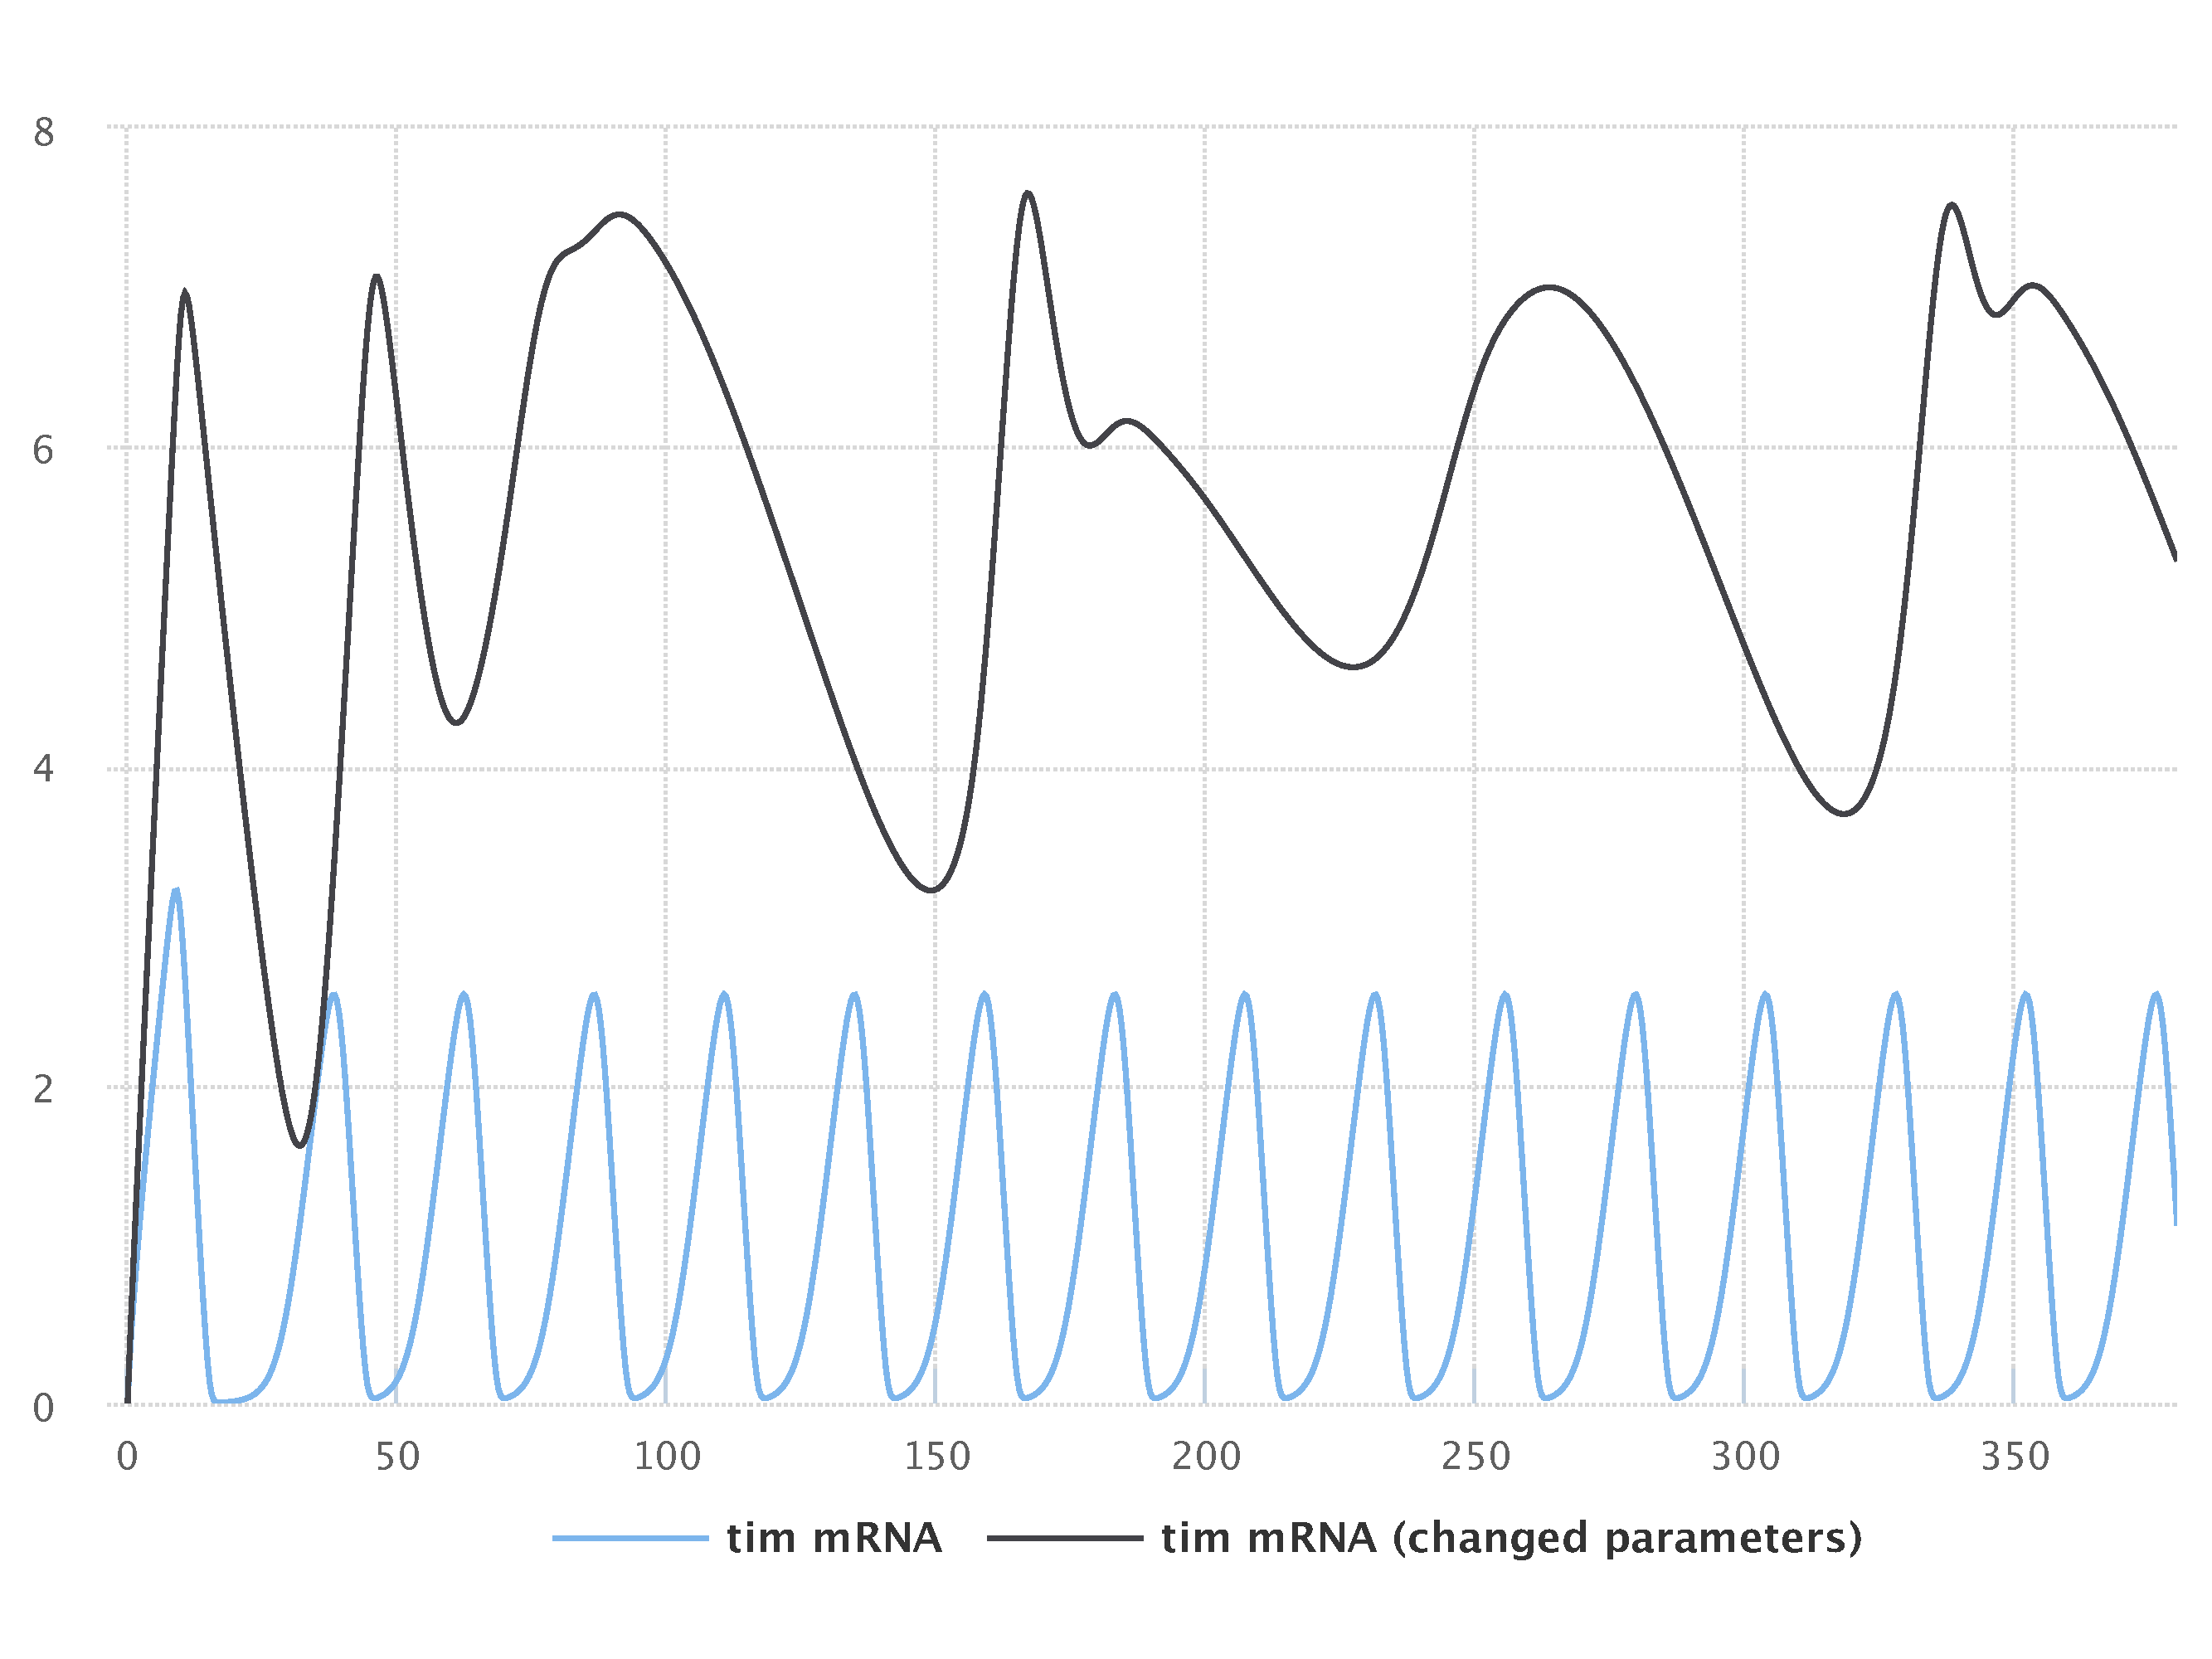
\includegraphics[width=1.0\textwidth]{examples/leloup-sbml/results/sedml_webtools/plot1}
		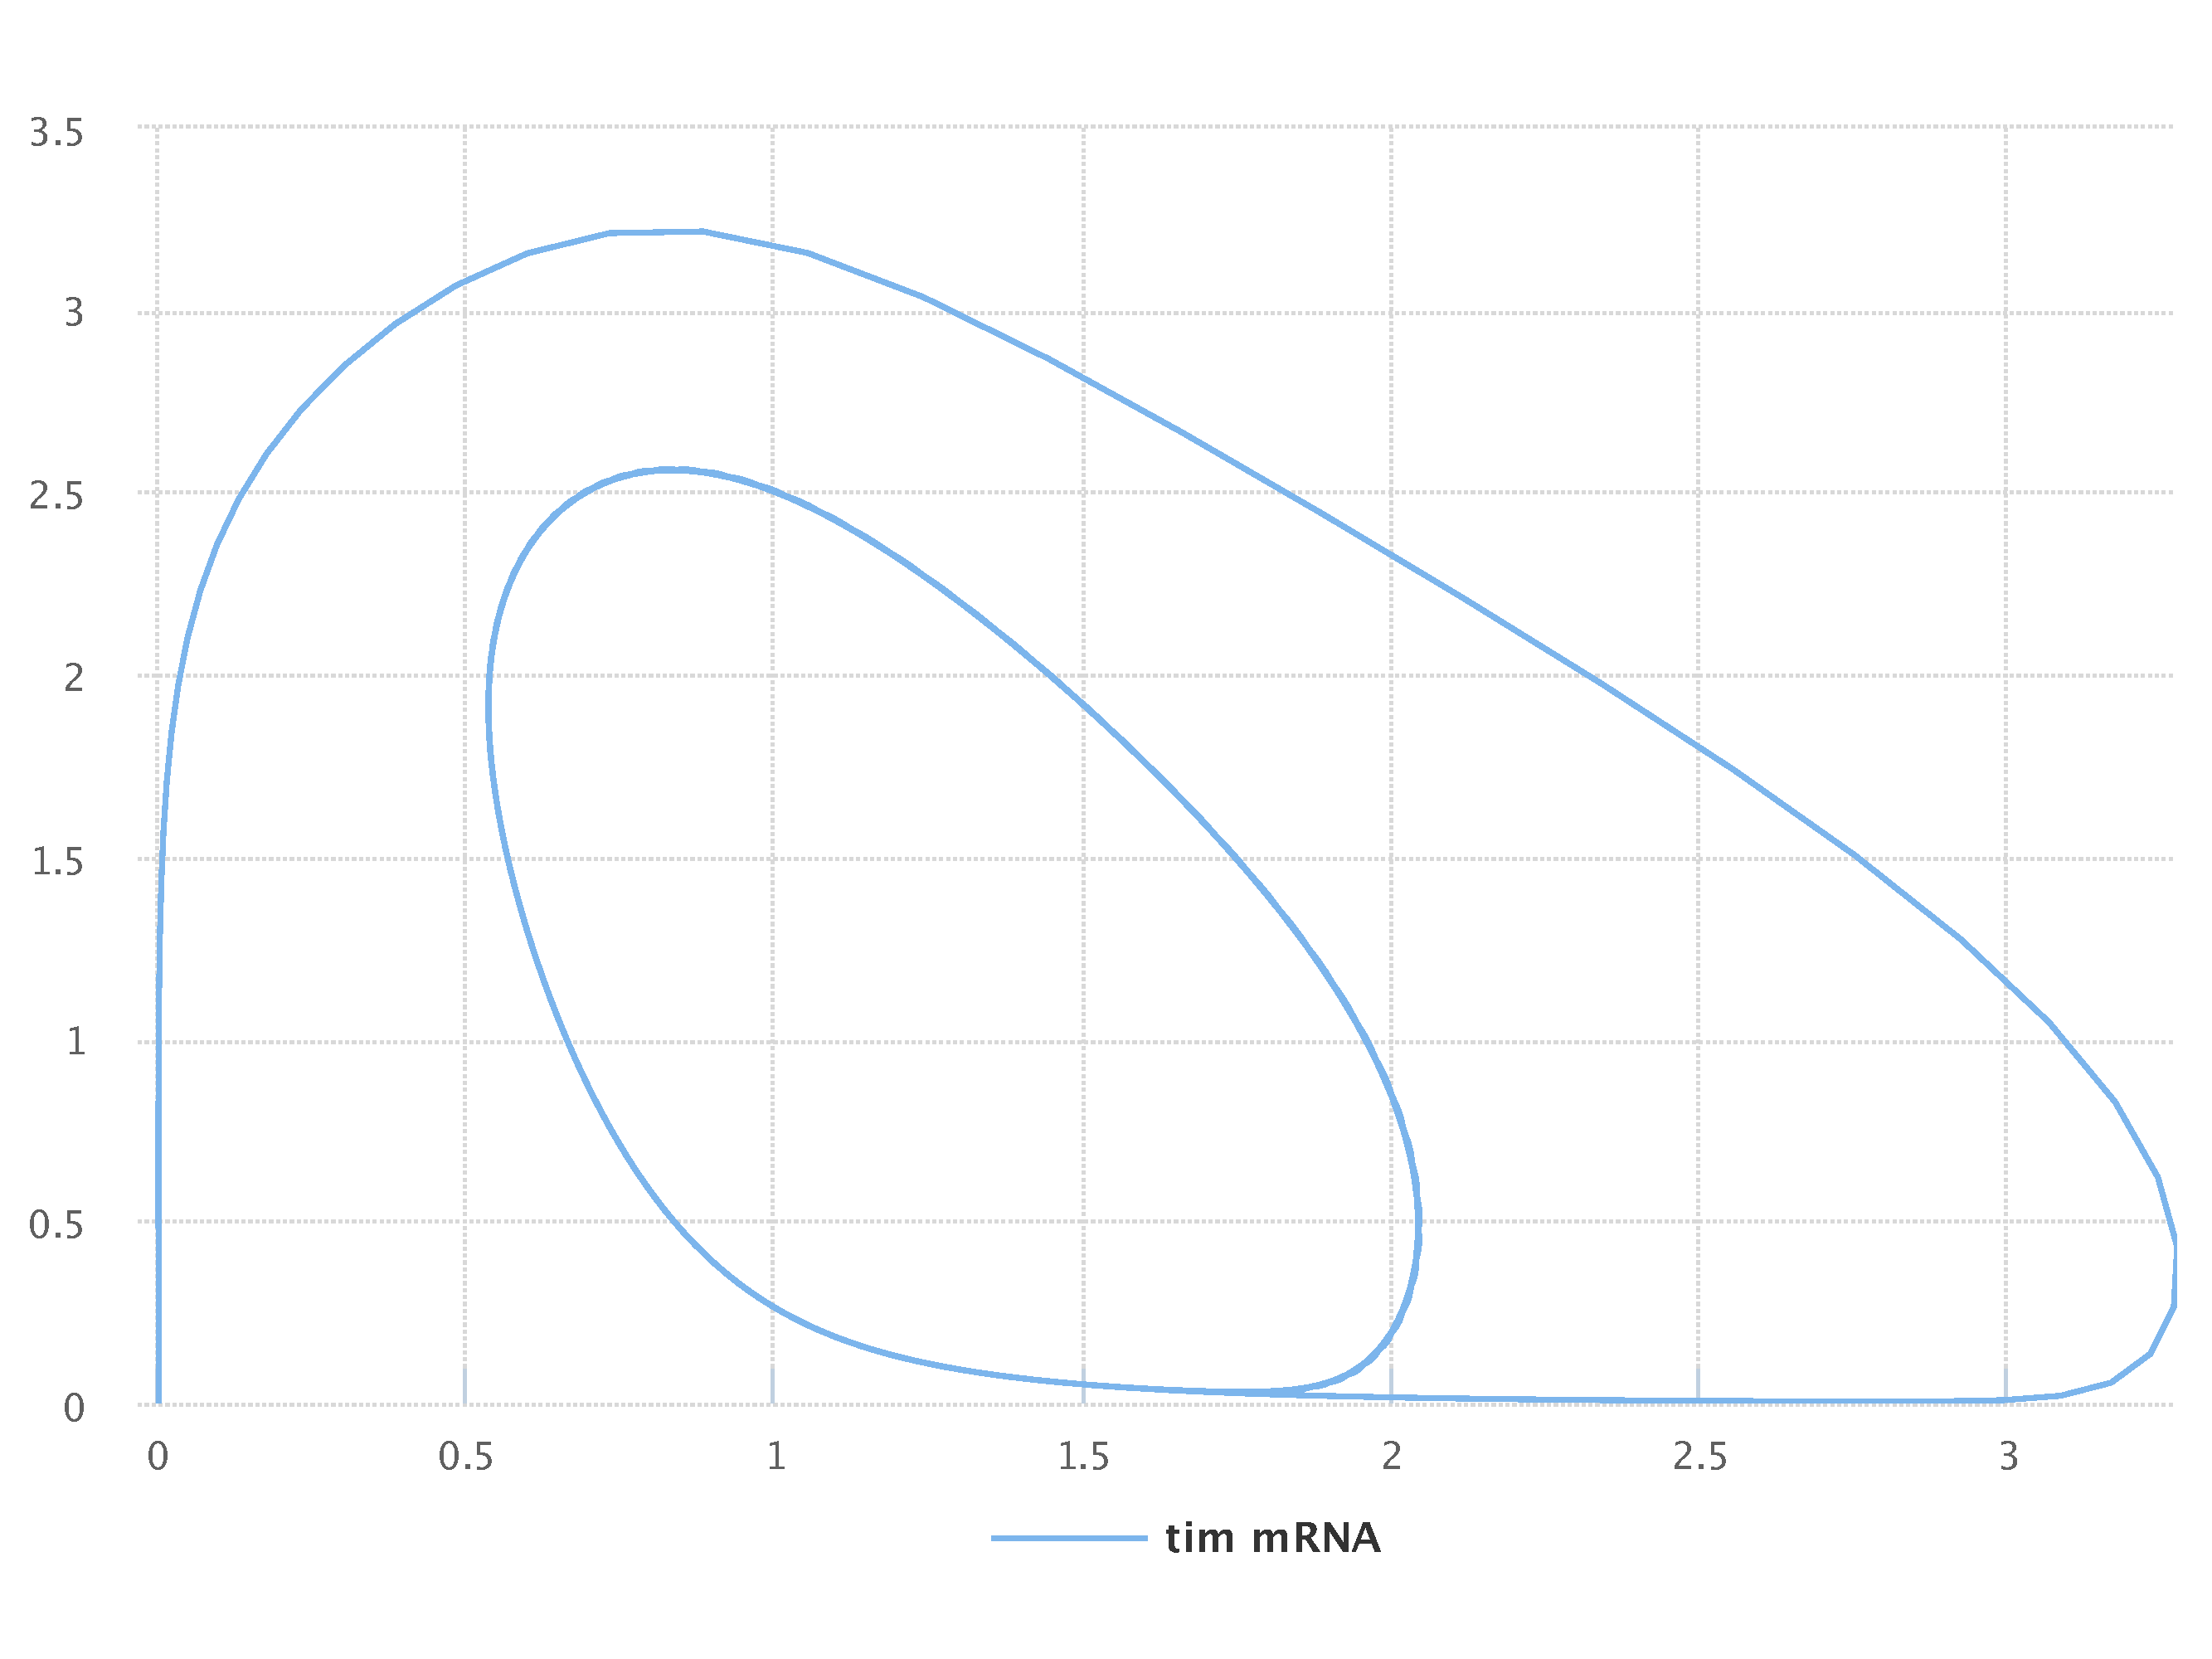
\includegraphics[width=1.0\textwidth]{examples/leloup-sbml/results/sedml_webtools/plot2}
		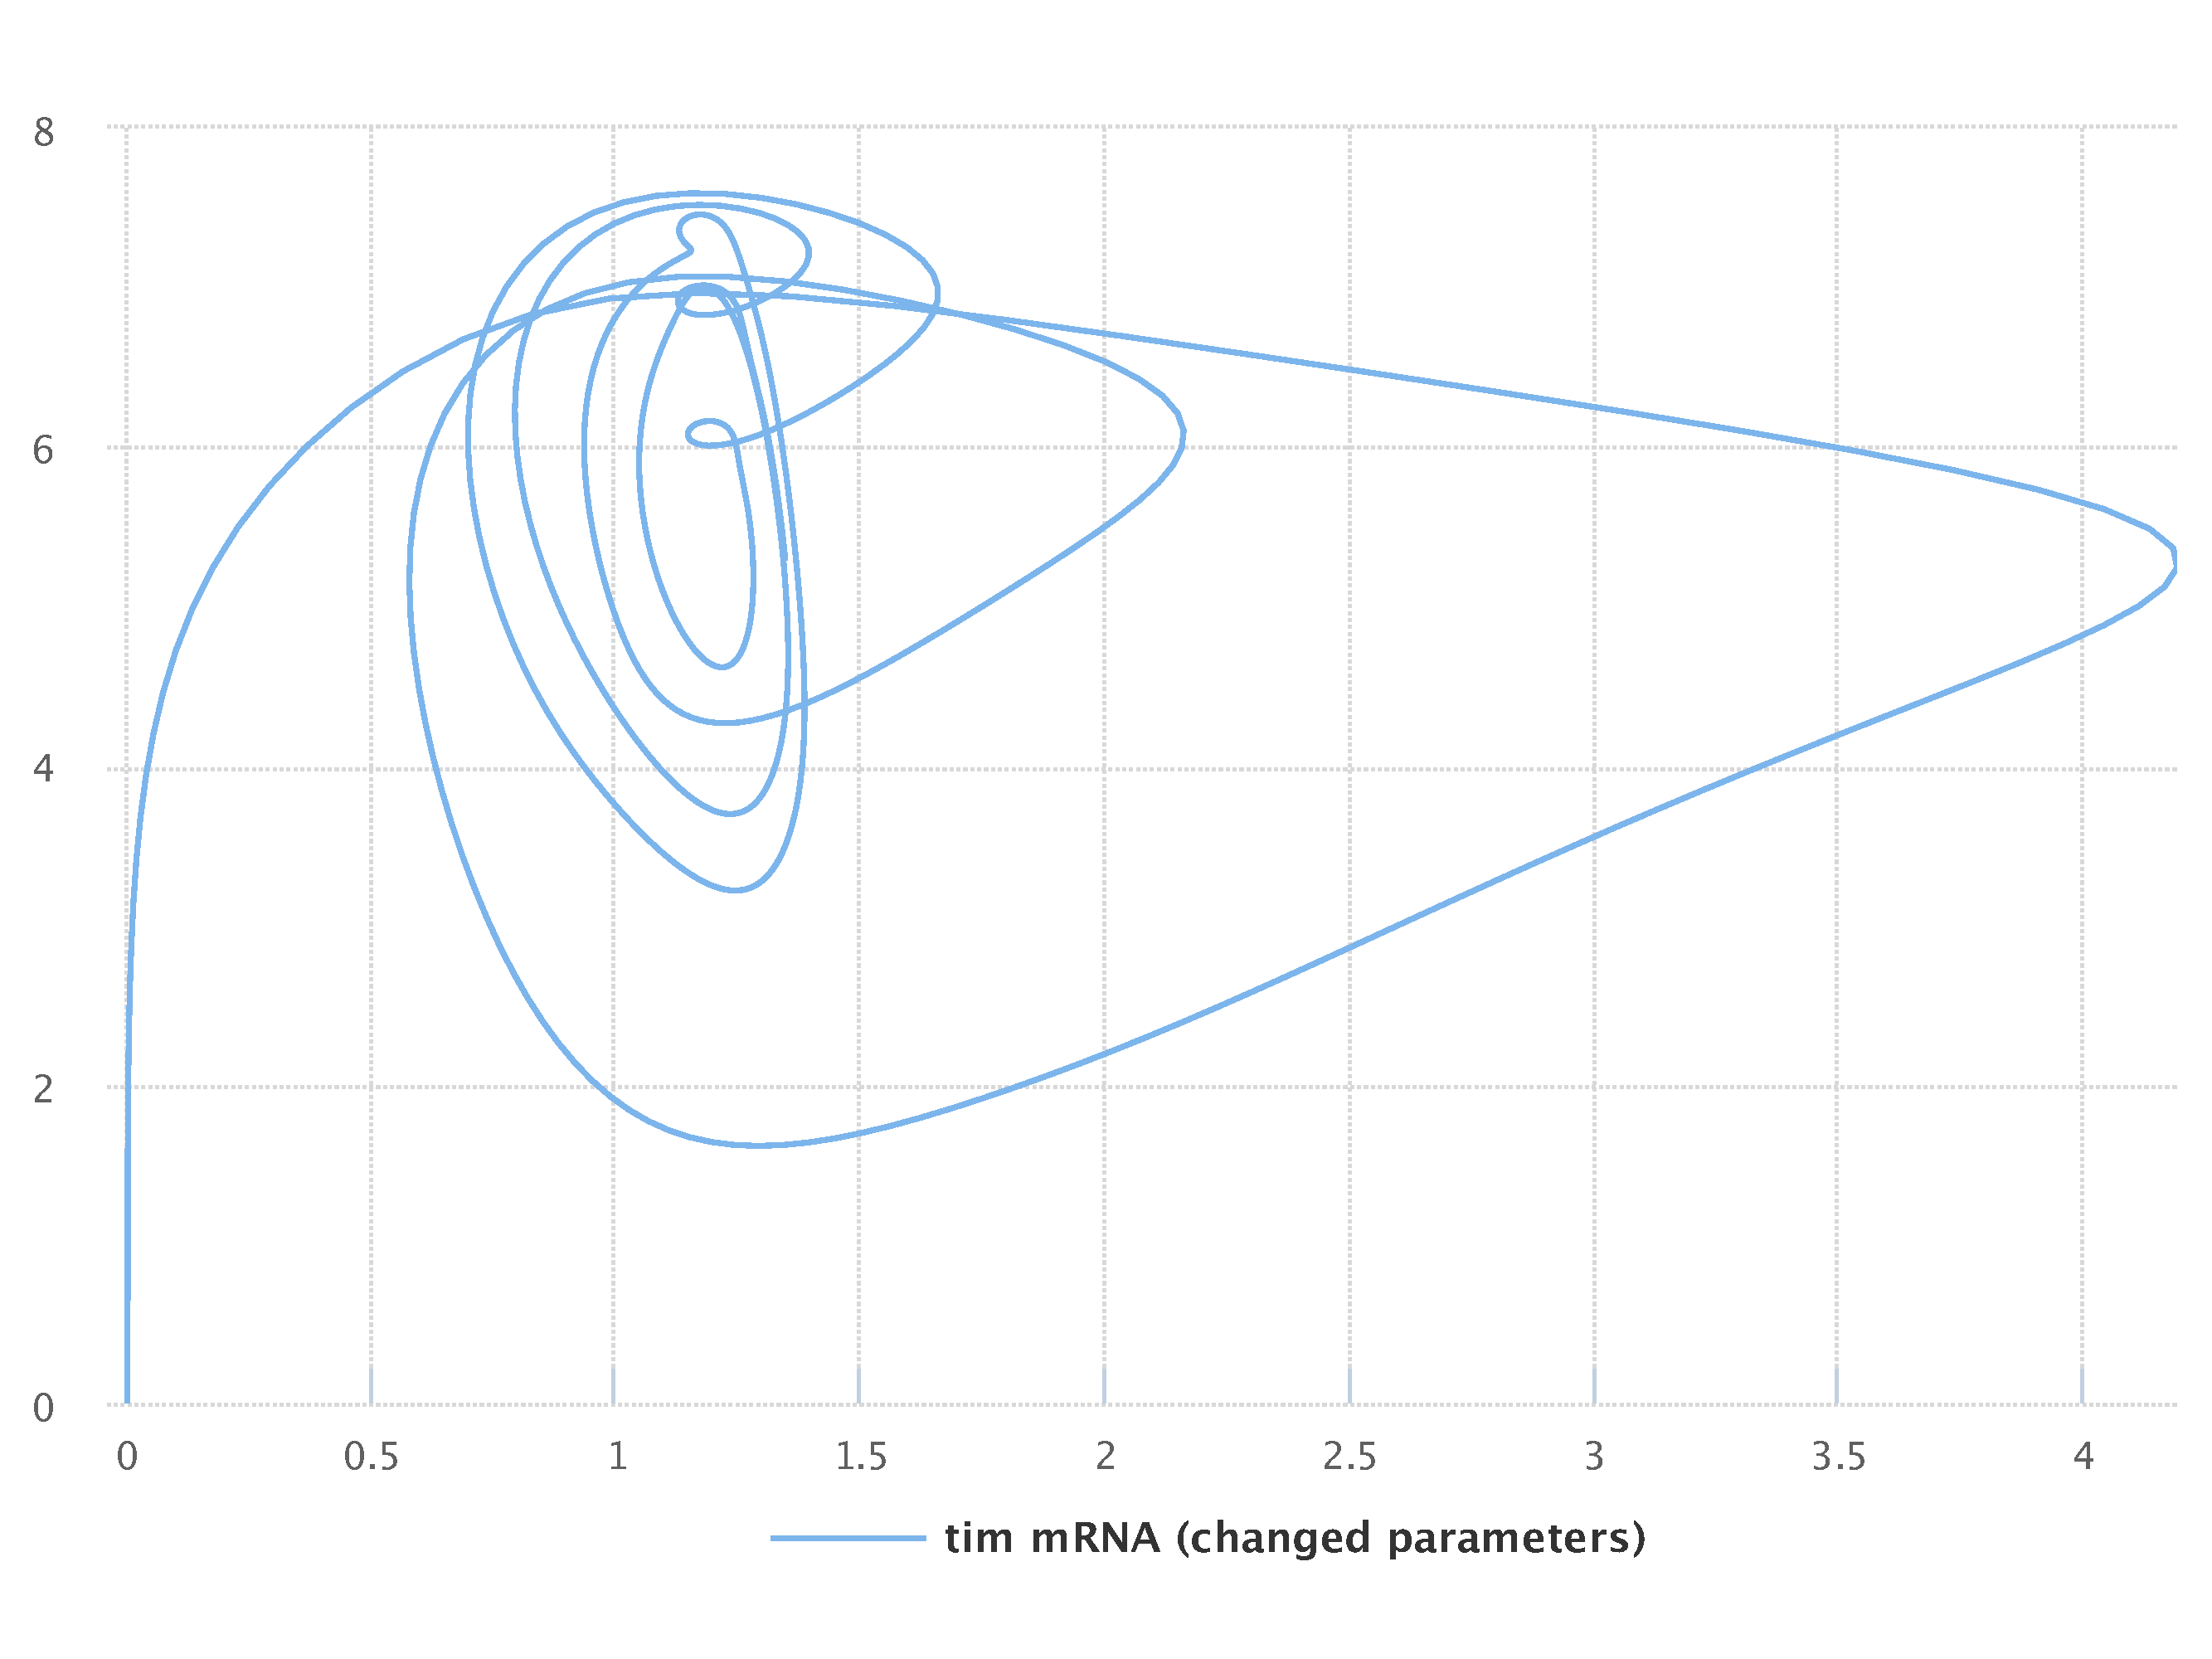
\includegraphics[width=1.0\textwidth]{examples/leloup-sbml/results/sedml_webtools/plot3}
        \caption{The simulation result gained from the simulation description given in \lst{leloup-sbml}. Simulation with SED-ML web tools \citep{bergmann2017sed}.}
        \label{fig:leloup-sbml1}
    \end{minipage}\hfill
    \begin{minipage}{0.47\textwidth}
        \centering
         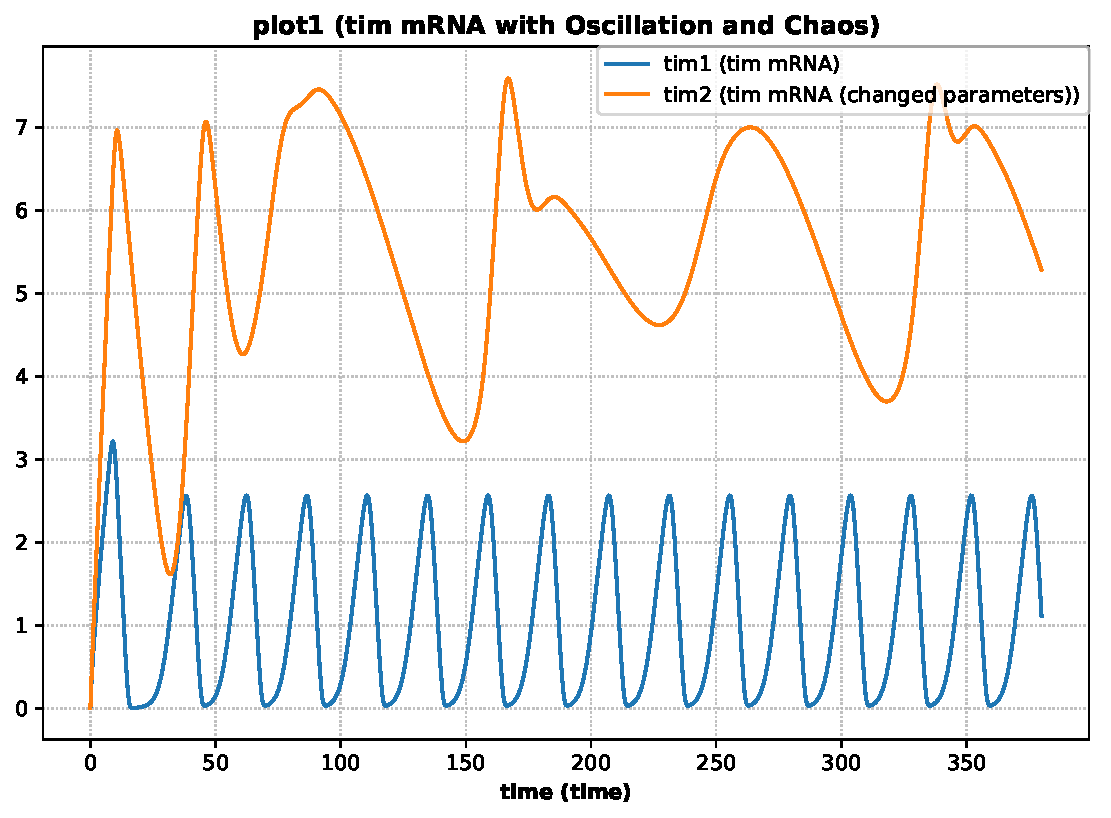
\includegraphics[width=1.0\textwidth]{examples/leloup-sbml/results/tellurium/plot1}
		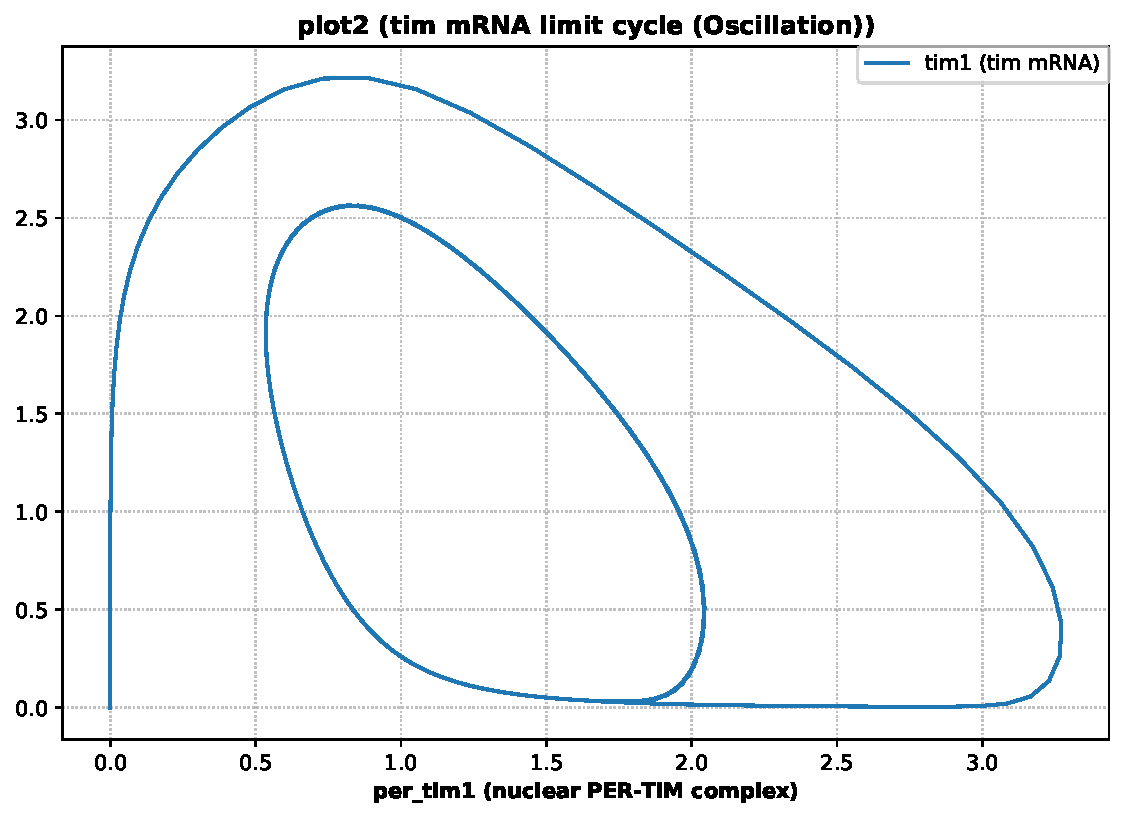
\includegraphics[width=1.0\textwidth]{examples/leloup-sbml/results/tellurium/plot2}
		\includegraphics[width=1.0\textwidth]{examples/leloup-sbml/results/tellurium/plot3}
        \caption{Simulation with tellurium \citep{tellurium}.}
        \label{fig:leloup-sbml2}
    \end{minipage}
    
\end{figure}

\myXmlImport{LeLoup Model Simulation Description in SED-ML}{lst:leloup-sbml}{examples/leloup-sbml/leloup-sbml.xml}


% ~~~ IKAPPAB ~~~
\subsection{IkappaB Signaling (\texttt{L1V3\_ikkapab.omex})}
The following example provides a SED-ML description for the simulation of the IkappaB-NF-kappaB signaling module described in \citep{hoffmann2002ikappab}.

This model is referenced by its SED-ML ID \code{model1} and refers to the model with the MIRIAM URN \url{urn:miriam:biomodels.db:BIOMD0000000140}. 
Software applications interpreting this example know how to dereference this URN and access the model in \biom \citep{N+06}.

The simulation description specifies one simulation \code{simulation1}, which is a uniform timecourse simulation that simulates the model for 41 hours. \code{task1} then applies this simulation to the model.

As output this simulation description collects four parameters: \code{Total\_NFkBn}, \code{Total\_IkBbeta}, \code{Total\_IkBeps} and \code{Total\_IkBalpha}. These variables are plotted against the simulation time as shown in Figure \ref{fig:ikappab1} and \ref{fig:ikappab2}.

\begin{figure}[ht]
    \centering
    \begin{minipage}{0.47\textwidth}
        \centering
        \includegraphics[width=1.0\textwidth]{examples/ikappab/results/sedml_webtools/plot1}
        \caption{The simulation result gained from the simulation description given in \lst{ikappab}. Simulation with SED-ML web tools \citep{bergmann2017sed}.}
        \label{fig:ikappab1}
    \end{minipage}\hfill
    \begin{minipage}{0.47\textwidth}
        \centering
        \includegraphics[width=1.0\textwidth]{examples/ikappab/results/tellurium/plot1}
        \caption{Simulation with tellurium \citep{tellurium}.}
        \label{fig:ikappab2}
    \end{minipage}
\end{figure}

\myXmlImport{IkappaB-NF-kappaB signaling Model Simulation Description in SED-ML}{lst:ikappab}{examples/ikappab/ikappab.xml}



% ~~~~~~~~~~~~~~~~~~~~~~~~~~~~~~~~~~~~
% XML SCHEMA
% ~~~~~~~~~~~~~~~~~~~~~~~~~~~~~~~~~~~~
\chapter{XML Schema}
\label{app:schema}
Listing \ref{lst:schema} shows the full SED-ML XML Schema.
\myXmlImport{The SED-ML XML Schema definition}{lst:schema}{schema/sed-ml-L1-V4.xsd}

% ~~~~~~~~~~~~~~~~~~~~~~~~~~~~~~~~~~~~
% REFERENCES
% ~~~~~~~~~~~~~~~~~~~~~~~~~~~~~~~~~~~~
\bibliographystyle{abbrv}
\bibliography{sed-ml}
\end{document}
